% Options for packages loaded elsewhere
\PassOptionsToPackage{unicode}{hyperref}
\PassOptionsToPackage{hyphens}{url}
\documentclass[
  10pt,
  b5paper,
  oneside]{book}
\usepackage{xcolor}
\usepackage{amsmath,amssymb}
\setcounter{secnumdepth}{5}
\usepackage{iftex}
\ifPDFTeX
  \usepackage[T1]{fontenc}
  \usepackage[utf8]{inputenc}
  \usepackage{textcomp} % provide euro and other symbols
\else % if luatex or xetex
  \usepackage{unicode-math} % this also loads fontspec
  \defaultfontfeatures{Scale=MatchLowercase}
  \defaultfontfeatures[\rmfamily]{Ligatures=TeX,Scale=1}
\fi
\usepackage{lmodern}
\ifPDFTeX\else
  % xetex/luatex font selection
\fi
% Use upquote if available, for straight quotes in verbatim environments
\IfFileExists{upquote.sty}{\usepackage{upquote}}{}
\IfFileExists{microtype.sty}{% use microtype if available
  \usepackage[]{microtype}
  \UseMicrotypeSet[protrusion]{basicmath} % disable protrusion for tt fonts
}{}
\makeatletter
\@ifundefined{KOMAClassName}{% if non-KOMA class
  \IfFileExists{parskip.sty}{%
    \usepackage{parskip}
  }{% else
    \setlength{\parindent}{0pt}
    \setlength{\parskip}{6pt plus 2pt minus 1pt}}
}{% if KOMA class
  \KOMAoptions{parskip=half}}
\makeatother
\usepackage{color}
\usepackage{fancyvrb}
\newcommand{\VerbBar}{|}
\newcommand{\VERB}{\Verb[commandchars=\\\{\}]}
\DefineVerbatimEnvironment{Highlighting}{Verbatim}{commandchars=\\\{\}}
% Add ',fontsize=\small' for more characters per line
\usepackage{framed}
\definecolor{shadecolor}{RGB}{248,248,248}
\newenvironment{Shaded}{\begin{snugshade}}{\end{snugshade}}
\newcommand{\AlertTok}[1]{\textcolor[rgb]{0.94,0.16,0.16}{#1}}
\newcommand{\AnnotationTok}[1]{\textcolor[rgb]{0.56,0.35,0.01}{\textbf{\textit{#1}}}}
\newcommand{\AttributeTok}[1]{\textcolor[rgb]{0.13,0.29,0.53}{#1}}
\newcommand{\BaseNTok}[1]{\textcolor[rgb]{0.00,0.00,0.81}{#1}}
\newcommand{\BuiltInTok}[1]{#1}
\newcommand{\CharTok}[1]{\textcolor[rgb]{0.31,0.60,0.02}{#1}}
\newcommand{\CommentTok}[1]{\textcolor[rgb]{0.56,0.35,0.01}{\textit{#1}}}
\newcommand{\CommentVarTok}[1]{\textcolor[rgb]{0.56,0.35,0.01}{\textbf{\textit{#1}}}}
\newcommand{\ConstantTok}[1]{\textcolor[rgb]{0.56,0.35,0.01}{#1}}
\newcommand{\ControlFlowTok}[1]{\textcolor[rgb]{0.13,0.29,0.53}{\textbf{#1}}}
\newcommand{\DataTypeTok}[1]{\textcolor[rgb]{0.13,0.29,0.53}{#1}}
\newcommand{\DecValTok}[1]{\textcolor[rgb]{0.00,0.00,0.81}{#1}}
\newcommand{\DocumentationTok}[1]{\textcolor[rgb]{0.56,0.35,0.01}{\textbf{\textit{#1}}}}
\newcommand{\ErrorTok}[1]{\textcolor[rgb]{0.64,0.00,0.00}{\textbf{#1}}}
\newcommand{\ExtensionTok}[1]{#1}
\newcommand{\FloatTok}[1]{\textcolor[rgb]{0.00,0.00,0.81}{#1}}
\newcommand{\FunctionTok}[1]{\textcolor[rgb]{0.13,0.29,0.53}{\textbf{#1}}}
\newcommand{\ImportTok}[1]{#1}
\newcommand{\InformationTok}[1]{\textcolor[rgb]{0.56,0.35,0.01}{\textbf{\textit{#1}}}}
\newcommand{\KeywordTok}[1]{\textcolor[rgb]{0.13,0.29,0.53}{\textbf{#1}}}
\newcommand{\NormalTok}[1]{#1}
\newcommand{\OperatorTok}[1]{\textcolor[rgb]{0.81,0.36,0.00}{\textbf{#1}}}
\newcommand{\OtherTok}[1]{\textcolor[rgb]{0.56,0.35,0.01}{#1}}
\newcommand{\PreprocessorTok}[1]{\textcolor[rgb]{0.56,0.35,0.01}{\textit{#1}}}
\newcommand{\RegionMarkerTok}[1]{#1}
\newcommand{\SpecialCharTok}[1]{\textcolor[rgb]{0.81,0.36,0.00}{\textbf{#1}}}
\newcommand{\SpecialStringTok}[1]{\textcolor[rgb]{0.31,0.60,0.02}{#1}}
\newcommand{\StringTok}[1]{\textcolor[rgb]{0.31,0.60,0.02}{#1}}
\newcommand{\VariableTok}[1]{\textcolor[rgb]{0.00,0.00,0.00}{#1}}
\newcommand{\VerbatimStringTok}[1]{\textcolor[rgb]{0.31,0.60,0.02}{#1}}
\newcommand{\WarningTok}[1]{\textcolor[rgb]{0.56,0.35,0.01}{\textbf{\textit{#1}}}}
\usepackage{longtable,booktabs,array}
\usepackage{calc} % for calculating minipage widths
% Correct order of tables after \paragraph or \subparagraph
\usepackage{etoolbox}
\makeatletter
\patchcmd\longtable{\par}{\if@noskipsec\mbox{}\fi\par}{}{}
\makeatother
% Allow footnotes in longtable head/foot
\IfFileExists{footnotehyper.sty}{\usepackage{footnotehyper}}{\usepackage{footnote}}
\makesavenoteenv{longtable}
\usepackage{graphicx}
\makeatletter
\newsavebox\pandoc@box
\newcommand*\pandocbounded[1]{% scales image to fit in text height/width
  \sbox\pandoc@box{#1}%
  \Gscale@div\@tempa{\textheight}{\dimexpr\ht\pandoc@box+\dp\pandoc@box\relax}%
  \Gscale@div\@tempb{\linewidth}{\wd\pandoc@box}%
  \ifdim\@tempb\p@<\@tempa\p@\let\@tempa\@tempb\fi% select the smaller of both
  \ifdim\@tempa\p@<\p@\scalebox{\@tempa}{\usebox\pandoc@box}%
  \else\usebox{\pandoc@box}%
  \fi%
}
% Set default figure placement to htbp
\def\fps@figure{htbp}
\makeatother
% definitions for citeproc citations
\NewDocumentCommand\citeproctext{}{}
\NewDocumentCommand\citeproc{mm}{%
  \begingroup\def\citeproctext{#2}\cite{#1}\endgroup}
\makeatletter
 % allow citations to break across lines
 \let\@cite@ofmt\@firstofone
 % avoid brackets around text for \cite:
 \def\@biblabel#1{}
 \def\@cite#1#2{{#1\if@tempswa , #2\fi}}
\makeatother
\newlength{\cslhangindent}
\setlength{\cslhangindent}{1.5em}
\newlength{\csllabelwidth}
\setlength{\csllabelwidth}{3em}
\newenvironment{CSLReferences}[2] % #1 hanging-indent, #2 entry-spacing
 {\begin{list}{}{%
  \setlength{\itemindent}{0pt}
  \setlength{\leftmargin}{0pt}
  \setlength{\parsep}{0pt}
  % turn on hanging indent if param 1 is 1
  \ifodd #1
   \setlength{\leftmargin}{\cslhangindent}
   \setlength{\itemindent}{-1\cslhangindent}
  \fi
  % set entry spacing
  \setlength{\itemsep}{#2\baselineskip}}}
 {\end{list}}
\usepackage{calc}
\newcommand{\CSLBlock}[1]{\hfill\break\parbox[t]{\linewidth}{\strut\ignorespaces#1\strut}}
\newcommand{\CSLLeftMargin}[1]{\parbox[t]{\csllabelwidth}{\strut#1\strut}}
\newcommand{\CSLRightInline}[1]{\parbox[t]{\linewidth - \csllabelwidth}{\strut#1\strut}}
\newcommand{\CSLIndent}[1]{\hspace{\cslhangindent}#1}
\setlength{\emergencystretch}{3em} % prevent overfull lines
\providecommand{\tightlist}{%
  \setlength{\itemsep}{0pt}\setlength{\parskip}{0pt}}
\usepackage{booktabs}
\usepackage{amsthm}
\makeatletter
\let\stdl@chapter\l@chapter
\renewcommand*{\l@chapter}[2]{%
  \stdl@chapter{\textcolor{astral}{#1}}{\textcolor{astral}{#2}}}

\def\thm@space@setup{%
  \thm@preskip=5cm
  \thm@postskip=\thm@preskip

}
\usepackage{graphicx}
\usepackage{afterpage}

\newcommand\blankpage{%
    \null
    \thispagestyle{empty}%
    \addtocounter{page}{-1}%
    \newpage}

\usepackage{amssymb}
\usepackage{amsmath}
%\pagestyle{plain} % default for report

\usepackage{etoolbox}
\makeatletter
\patchcmd{\@makechapterhead}{50\p@}{-24pt}{}{}
\patchcmd{\@makeschapterhead}{50\p@}{-24pt}{}{}
\makeatother

\makeatother
\usepackage{sectsty}

\definecolor{astral}{RGB}{153, 61, 15}
\allsectionsfont{\sffamily\color{astral}}


\usepackage{fancyhdr}
\usepackage{pdfpages}

\renewcommand{\headrulewidth}{0.5pt}
\renewcommand{\headrule}{\hbox to\headwidth{\color{astral}\leaders\hrule height \headrulewidth\hfill}}


\setlength{\headheight}{5pt}

\fancyhf{}
\fancyhead[EL]{\nouppercase\leftmark}
\fancyhead[OR]{\nouppercase\rightmark}
\fancyhead[ER,OL]{\thepage}

\usepackage{multicol}
\usepackage{hyperref}
\usepackage{longtable}
\usepackage{array}
\usepackage{multirow}
\usepackage{wrapfig}
\usepackage{float}
\usepackage{colortbl}
\usepackage{pdflscape}
\usepackage{tabu}
\usepackage{threeparttable}
\usepackage{adjustbox}
\usepackage{rotating}
\usepackage{tablefootnote}
\usepackage[normalem]{ulem}
% empty pages betwen chapters
\usepackage{emptypage}


\makeatletter
\makeatother

\renewcommand{\listfigurename}{Figures}
\renewcommand{\listtablename}{Tables}

\usepackage[sectionbib]{chapterbib}

%% List of Abbreviations
\usepackage{nomencl}
\makenomenclature
\renewcommand{\nomname}{Acronyms}
%% to update run makeindex on docs folder and move results to / folder
%% see nomencl manual
%% e.g. makeindex SOCMapping.nlo -s nomencl.ist -o SOCMapping.nls

%% index
\usepackage{imakeidx}
\makeindex

\usepackage{xspace}

% no title page
\AtBeginDocument{\let\maketitle\relax}
\hypersetup{
	colorlinks=true,
	linkcolor=astral,
	filecolor=astral,
	urlcolor=astral,
	citecolor=astral
}

\AtBeginDocument{\renewcommand{\chaptername}{Chapter}}
\usepackage{titling}
\usepackage{natbib}
\usepackage{pdfpages}
\usepackage{fancyhdr}
\usepackage{booktabs}
\usepackage{longtable}
\usepackage{subfig}
\usepackage{array}
\usepackage{amsmath}
\usepackage{multirow}
\usepackage{wrapfig}
\usepackage{bookmark}
\usepackage[utf8]{inputenc}
\usepackage{float}
\usepackage{colortbl}
\usepackage{pdflscape}
\usepackage{tabu}
\usepackage{threeparttable}
\usepackage{threeparttablex}
\usepackage[normalem]{ulem}
\usepackage{makecell}
\usepackage{xcolor}
\DeclareUnicodeCharacter{2212}{\textendash}
\usepackage{rotating, graphicx}
\usepackage{listings}
\usepackage{bookmark}
\IfFileExists{xurl.sty}{\usepackage{xurl}}{} % add URL line breaks if available
\urlstyle{same}
\hypersetup{
  pdftitle={DRAFT - Integrated soil information for decision-making },
  pdfauthor={Angelini, M.E., Rodriguez Lado, L., Mendes, W. S., Ribeiro, E., Luotto, I., Wadoux, A. M.J.-C, Ramirez-Lopez, L},
  hidelinks,
  pdfcreator={LaTeX via pandoc}}

\title{DRAFT - Integrated soil information for decision-making}
\usepackage{etoolbox}
\makeatletter
\providecommand{\subtitle}[1]{% add subtitle to \maketitle
  \apptocmd{\@title}{\par {\large #1 \par}}{}{}
}
\makeatother
\subtitle{Guided R tutorials covering the soil information and data lifecycle, from soil sampling design and mapping to data-driven decision-making.}
\author{Angelini, M.E., Rodriguez Lado, L., Mendes, W. S., Ribeiro, E., Luotto, I., Wadoux, A. M.J.-C, Ramirez-Lopez, L}
\date{}

\begin{document}
\maketitle

\pagestyle{plain}

\includepdf{images/frontcover.pdf}
\afterpage{\blankpage}
\thispagestyle{empty}
\begin{titlepage}
    \begin{center}
        \vspace*{4cm}
        \Large

        \textcolor{astral}{\textbf{Global Soil Nutrient and Nutrient Budgets maps (GSNmap) Phase I\\
Technical Manual\\}}
        \vspace{0.5cm}
        \normalsize
        \vfill
        \noindent
        {\color{astral}\rule{\linewidth}{0.5mm} }

        Food and Agriculture Organization of the United Nations\\
	Rome, 2022
    \end{center}
\end{titlepage}
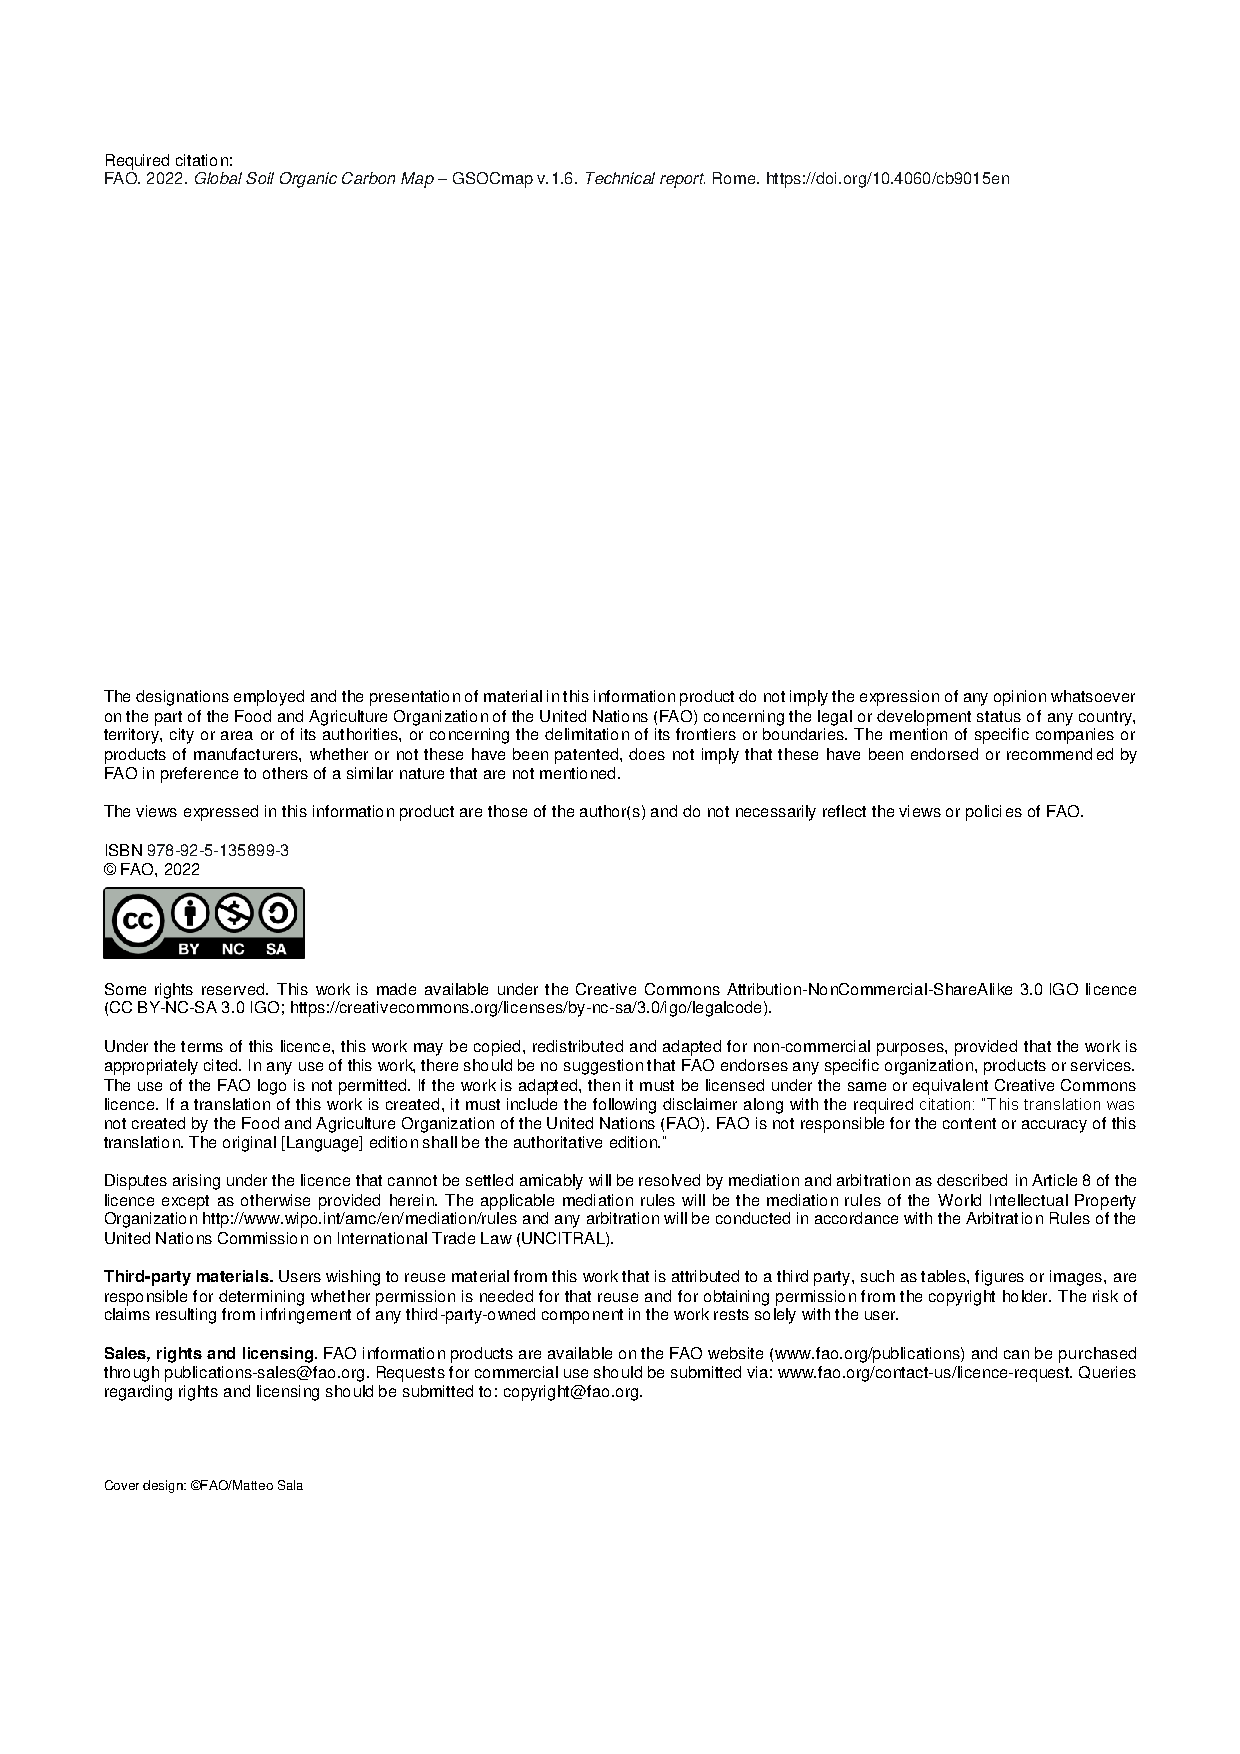
\includepdf{images/CB9015EN-Copyright-Disclaimer-v2.pdf}

\chapter{(PDF disabled)}\label{pdf-disabled}

Placeholder

\chapter*{Presentation and basics}\label{presentation-and-basics}
\addcontentsline{toc}{chapter}{Presentation and basics}

Placeholder

\section*{The Training Dataset}\label{the-training-dataset}
\addcontentsline{toc}{section}{The Training Dataset}

\subsection*{Data Structure}\label{data-structure}
\addcontentsline{toc}{subsection}{Data Structure}

\section*{How to Use This Manual}\label{how-to-use-this-manual}
\addcontentsline{toc}{section}{How to Use This Manual}

\subsection*{Manual Structure}\label{manual-structure}
\addcontentsline{toc}{subsection}{Manual Structure}

\subsubsection*{\texorpdfstring{\textbf{Module 1: Introduction to R and Preparation of Soil Data for Digital Soil Mapping}}{Module 1: Introduction to R and Preparation of Soil Data for Digital Soil Mapping}}\label{module-1-introduction-to-r-and-preparation-of-soil-data-for-digital-soil-mapping}
\addcontentsline{toc}{subsubsection}{\textbf{Module 1: Introduction to R and Preparation of Soil Data for Digital Soil Mapping}}

\subsubsection*{\texorpdfstring{\textbf{Module 2: Soil Sampling Design}}{Module 2: Soil Sampling Design}}\label{module-2-soil-sampling-design}
\addcontentsline{toc}{subsubsection}{\textbf{Module 2: Soil Sampling Design}}

\subsubsection*{\texorpdfstring{\textbf{Module 3: Digital Soil Mapping}}{Module 3: Digital Soil Mapping}}\label{module-3-digital-soil-mapping}
\addcontentsline{toc}{subsubsection}{\textbf{Module 3: Digital Soil Mapping}}

\subsubsection*{\texorpdfstring{\textbf{Module 4: Soil Spectroscopy}}{Module 4: Soil Spectroscopy}}\label{module-4-soil-spectroscopy}
\addcontentsline{toc}{subsubsection}{\textbf{Module 4: Soil Spectroscopy}}

\subsubsection*{\texorpdfstring{\textbf{Module 5: Soil Data Standardisation, Sharing and Dissemination}}{Module 5: Soil Data Standardisation, Sharing and Dissemination}}\label{module-5-soil-data-standardisation-sharing-and-dissemination}
\addcontentsline{toc}{subsubsection}{\textbf{Module 5: Soil Data Standardisation, Sharing and Dissemination}}

\section*{Required downloads}\label{required-downloads}
\addcontentsline{toc}{section}{Required downloads}

\subsection*{Step-by-step setup instructions}\label{step-by-step-setup-instructions}
\addcontentsline{toc}{subsection}{Step-by-step setup instructions}

\subsubsection*{Step 1: Download and extract the GitHub repository}\label{step-1-download-and-extract-the-github-repository}
\addcontentsline{toc}{subsubsection}{Step 1: Download and extract the GitHub repository}

\subsubsection*{Step 2: Download the Google Drive data}\label{step-2-download-the-google-drive-data}
\addcontentsline{toc}{subsubsection}{Step 2: Download the Google Drive data}

\subsubsection*{Step 3: Inspect the project folder structure}\label{step-3-inspect-the-project-folder-structure}
\addcontentsline{toc}{subsubsection}{Step 3: Inspect the project folder structure}

\subsubsection*{Step 4: Place Google Drive files into the correct module folders}\label{step-4-place-google-drive-files-into-the-correct-module-folders}
\addcontentsline{toc}{subsubsection}{Step 4: Place Google Drive files into the correct module folders}

\section*{Installing R and RStudio}\label{installing-r-and-rstudio}
\addcontentsline{toc}{section}{Installing R and RStudio}

\subsection{Installing R}\label{installing-r}

\subsection{Installing RStudio}\label{installing-rstudio}

\subsection{Verifying Installation}\label{verifying-installation}

\section*{Setting Up Google Earth Engine}\label{setting-up-google-earth-engine}
\addcontentsline{toc}{section}{Setting Up Google Earth Engine}

\subsection{Step 1: Create a Google Account}\label{step-1-create-a-google-account}

\subsection{Step 2: Register for a GEE Account}\label{step-2-register-for-a-gee-account}

\subsection{Step 3: Create or Select a Google Cloud Project}\label{step-3-create-or-select-a-google-cloud-project}

\subsection{Step 4: Access the GEE Code Editor}\label{step-4-access-the-gee-code-editor}

\subsubsection{Left Panel: Scripts, Assets, and Documentation}\label{left-panel-scripts-assets-and-documentation}

\subsubsection{Central Panel: The Code Editor}\label{central-panel-the-code-editor}

\subsubsection{Right Panel: Console, Inspector, and Tasks}\label{right-panel-console-inspector-and-tasks}

\subsubsection{Lower Section: The Interactive Map}\label{lower-section-the-interactive-map}

\subsection{Step 5: Prepare Your Google Drive Export Folder}\label{step-5-prepare-your-google-drive-export-folder}

\section*{Installation of QGIS}\label{installation-of-qgis}
\addcontentsline{toc}{section}{Installation of QGIS}

\subsection{Windows}\label{windows}

\subsection{macOS / Linux}\label{macos-linux}

\chapter{Introduction to Soil Data Preparation \& Spatial Data}\label{introduction-to-soil-data-preparation-spatial-data}

\section{Introduction to R}\label{introduction-to-r}

\subsection{Understanding the RStudio Interface}\label{understanding-the-rstudio-interface}

\textbf{RStudio} provides an integrated environment that simplifies working with R. The interface is divided into four main panes (Fig. \ref{fig:rstudio}):

\begin{figure}
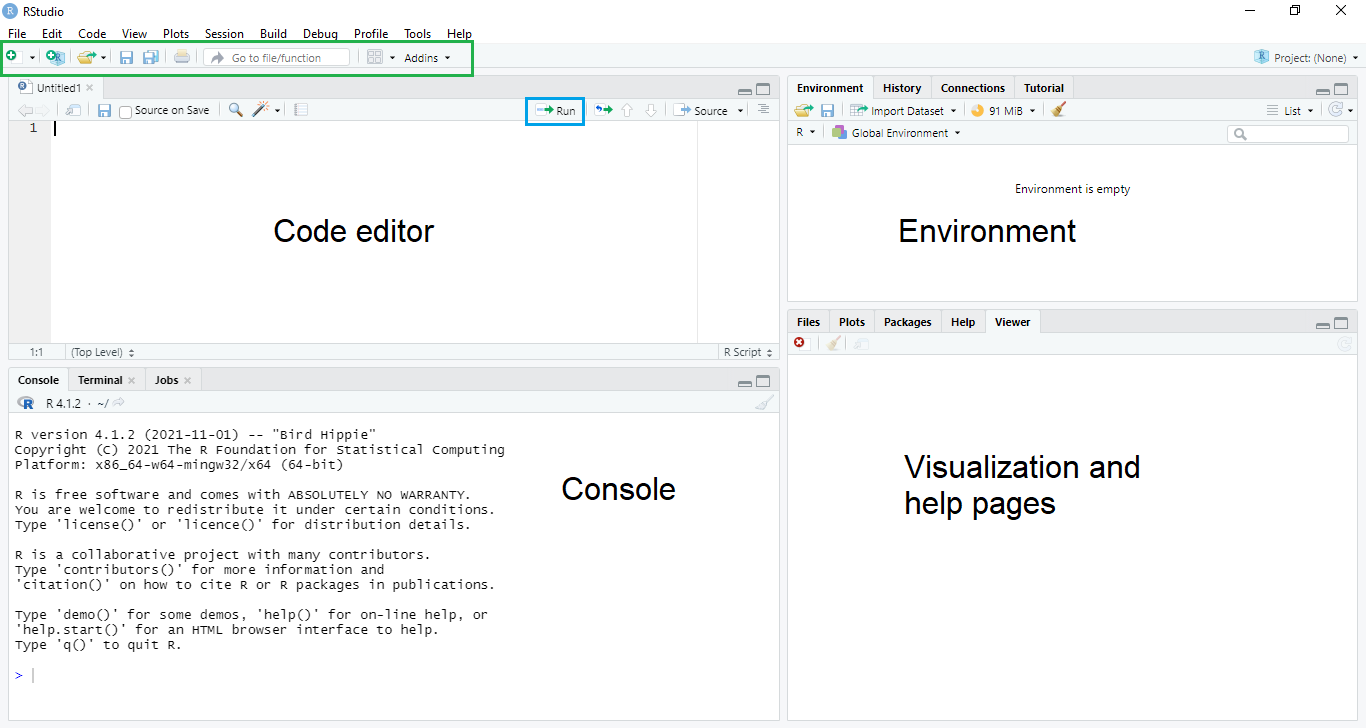
\includegraphics[width=1\linewidth]{images/module1/RStudio-interface} \caption{RStudio interface.}\label{fig:rstudio}
\end{figure}

The \textbf{Console} (Bottom Left) is where R code is executed.
You can type commands directly here or run them from your script.
The Console displays results, warnings, and error messages.

\begin{Shaded}
\begin{Highlighting}[]
\CommentTok{\# Type directly in the console}
\DecValTok{5} \SpecialCharTok{*} \DecValTok{3}

\CommentTok{\# R will immediately show the result}
\CommentTok{\# [1] 15}
\end{Highlighting}
\end{Shaded}

You can write commands directly in the Console (Top Left) and execute them line by line. However, it is usually more convenient to write code in a script editor---the \textbf{Code Editor} pane. Here you can create and edit R scripts (\texttt{.R} files), R Markdown documents (\texttt{.Rmd} files), and other file types. Scripts allow you to save your code and run it repeatedly, which is essential for reproducible analysis.

Working in the \textbf{Code Editor} also makes it easier to organize code for later use. You can send any line or selected block of code to the \textbf{Console} for execution by pressing \texttt{Ctrl\ +\ Enter} (Windows/Linux) or \texttt{Cmd\ +\ Enter} (macOS). You can also run code by clicking the \textbf{Run} button in the top-right corner of the \textbf{Code Editor} pane.

\begin{itemize}
\tightlist
\item
  Code can be written and executed directly in the \textbf{Console}.\\
\item
  Using the \textbf{Code Editor} is more convenient for organizing and reusing code.\\
\item
  Send a line or block of code to the console with \texttt{Ctrl\ +\ Enter} (Windows), \texttt{Cmd\ +\ Enter} (macOS), or the equivalent shortcut in Linux.\\
\item
  You can also run code by clicking the \textbf{Run} button in the script editor.\\
\end{itemize}

\textbf{Creating a new script:}
- File → New File → R Script (or press \texttt{Ctrl+Shift+N} / \texttt{Cmd+Shift+N})

Top Right Pane (Environment/History) is divided into:

\begin{itemize}
\item
  \textbf{Environment}: Shows all objects (variables, datasets, functions) currently in your R session
\item
  \textbf{History}: Records all commands you've run during the session
\end{itemize}

Finally, the Bottom Right Pane shows

\begin{itemize}
\item
  \textbf{Files}: Browse your computer's file system
\item
  \textbf{Plots}: View visualizations created with R
\item
  \textbf{Packages}: Manage installed packages
\item
  \textbf{Help}: Access R documentation and function help pages
\end{itemize}

\textbf{Best Practice}

\begin{itemize}
\item
  Always work in scripts rather than typing directly in the Console.
\item
  Scripts preserve your workflow and make your analysis reproducible.
\end{itemize}

\subsection{R Packages: Extending R's Capabilities}\label{r-packages-extending-rs-capabilities}

R's strength lies in its extensibility through \textbf{packages}.
A package is a collection of functions, data, and documentation that extends R's functionality for specific tasks.

\subsubsection{What are Packages?}\label{what-are-packages}

The base R installation includes fundamental functions for data manipulation and statistical analysis.
However, specialized tasks often require additional tools provided by contributed packages.

For soil science work, key packages include:

\begin{itemize}
\item
  \texttt{\{tidyverse\}}: A collection of packages for data manipulation and visualization, including \texttt{\{dplyr\}} and \texttt{\{tidyr\}}, among others
\item
  \texttt{\{terra\}}: Spatial data analysis and raster operations
\item
  \texttt{\{sf\}}: Working with vector spatial data
\item
  \texttt{\{aqp\}}: Algorithms for Quantitative Pedology (soil profile data)
\item
  \texttt{\{ggplot2\}}: Advanced data visualization (part of tidyverse)
\end{itemize}

\subsubsection{Installing Packages}\label{installing-packages}

Packages need to be installed once before you can use them.
Use \texttt{install.packages()}:

\begin{Shaded}
\begin{Highlighting}[]
\CommentTok{\# Install a single package}
\FunctionTok{install.packages}\NormalTok{(}\StringTok{"tidyverse"}\NormalTok{)}

\CommentTok{\# Install multiple packages at once}
\FunctionTok{install.packages}\NormalTok{(}\FunctionTok{c}\NormalTok{(}\StringTok{"terra"}\NormalTok{, }\StringTok{"sf"}\NormalTok{, }\StringTok{"aqp"}\NormalTok{))}
\end{Highlighting}
\end{Shaded}

You only need to install a package once, but you must load it with \texttt{library()} each time you start a new R session.

You can check which \emph{\{packages\}} are installed with:

\begin{Shaded}
\begin{Highlighting}[]
\FunctionTok{installed.packages}\NormalTok{()}
\end{Highlighting}
\end{Shaded}

\paragraph*{Install Packages from GitHub or Other Sources}\label{install-packages-from-github-or-other-sources}
\addcontentsline{toc}{paragraph}{Install Packages from GitHub or Other Sources}

Some \emph{\{packages\}} are not yet available on CRAN or you may want newer development versions from GitHub, Gitlab, bitbucket, or an URL.
In these cases, you can use the \texttt{remotes} or \texttt{devtools} \emph{\{packages\}}, with the functions \texttt{install\_github()}, \texttt{install\_gitlab()}, \texttt{install\_bitbucket()} or \texttt{install\_url()}:

\begin{Shaded}
\begin{Highlighting}[]
\CommentTok{\# First, install remotes package (if not already installed)}
\FunctionTok{install.packages}\NormalTok{(}\StringTok{"remotes"}\NormalTok{)}

\CommentTok{\# Install an R package from GitHub}
\NormalTok{remotes}\SpecialCharTok{::}\FunctionTok{install\_github}\NormalTok{(}\StringTok{"rspatial/terra"}\NormalTok{)}
\end{Highlighting}
\end{Shaded}

This is useful for accessing cutting-edge versions, experimental features, or tools developed by research groups.

\paragraph*{Manual Installation of R Packages}\label{manual-installation-of-r-packages}
\addcontentsline{toc}{paragraph}{Manual Installation of R Packages}

You may need to install R \emph{\{packages\}} manually, especially when working in environments without internet access or when using custom-built \emph{\{packages\}}.

There are two common methods:

\begin{itemize}
\tightlist
\item
  \textbf{1. Installing from a compressed source package file} (e.g., \texttt{mypackage\_1.0.0.tar.gz})
\end{itemize}

\begin{Shaded}
\begin{Highlighting}[]
\FunctionTok{install.packages}\NormalTok{(}\StringTok{"path/to/mypackage\_1.0.0.tar.gz"}\NormalTok{, }\AttributeTok{repos =} \ConstantTok{NULL}\NormalTok{, }\AttributeTok{type =} \StringTok{"source"}\NormalTok{)}
\end{Highlighting}
\end{Shaded}

\begin{itemize}
\tightlist
\item
  \textbf{2. Installing from a Local \texttt{.zip} file} (Windows Binary)
\end{itemize}

\begin{Shaded}
\begin{Highlighting}[]
\FunctionTok{install.packages}\NormalTok{(}\StringTok{"path/to/mypackage.zip"}\NormalTok{, }\AttributeTok{repos =} \ConstantTok{NULL}\NormalTok{, }\AttributeTok{type =} \StringTok{"win.binary"}\NormalTok{)}
\end{Highlighting}
\end{Shaded}

This method does not require compilation and is usually faster on Windows.

\textbf{Note:}

\begin{itemize}
\item
  Package installation typically requires an internet connection.
\item
  Depending on the package size and your connection speed, installation may take several minutes.
\end{itemize}

\subsubsection{Loading Packages}\label{loading-packages}

After installation, you must \textbf{load} a package into your R session each time you start R.
Use the \texttt{library()} function:

\begin{Shaded}
\begin{Highlighting}[]
\CommentTok{\# Load tidyverse package}
\FunctionTok{library}\NormalTok{(tidyverse)}

\CommentTok{\# Load multiple packages}
\FunctionTok{library}\NormalTok{(terra)}
\FunctionTok{library}\NormalTok{(sf)}
\FunctionTok{library}\NormalTok{(aqp)}
\end{Highlighting}
\end{Shaded}

\textbf{Key Difference:}

\begin{itemize}
\tightlist
\item
  \texttt{install.packages()}: Downloads and installs a package (once)
\item
  \texttt{library()}: Loads a package into your current session (every time you start R)
\end{itemize}

\subsubsection{Finding Help on Packages}\label{finding-help-on-packages}

\begin{Shaded}
\begin{Highlighting}[]
\CommentTok{\# Get help on a package}
\FunctionTok{help}\NormalTok{(}\AttributeTok{package =} \StringTok{"tidyverse"}\NormalTok{)}

\CommentTok{\# Or use}
\NormalTok{?tidyverse}

\CommentTok{\# View vignettes (tutorials) for a package}
\FunctionTok{vignette}\NormalTok{(}\AttributeTok{package =} \StringTok{"ggplot2"}\NormalTok{)}
\FunctionTok{vignette}\NormalTok{(}\StringTok{"ggplot2"}\NormalTok{, }\AttributeTok{package =} \StringTok{"ggplot2"}\NormalTok{)}
\end{Highlighting}
\end{Shaded}

\subsection{R Basics: Objects and Data Types}\label{object-types}

In R, everything you work with is an \textbf{object} (numbers, text, vectors, tables, models, and maps). When you create an object, R stores it in your computer's \textbf{memory} (RAM) so you can reuse it later. Because memory is limited, especially when working with large soil datasets, rasters, or spatial objects, it is good practice to keep your workspace tidy: reuse objects when appropriate, remove objects you no longer need with \texttt{rm()}, and occasionally trigger garbage collection with ´gc()´ to free memory that is no longer in use.

\subsubsection{Creating Objects with Assignment}\label{object-assignment}

If you run an operation without assigning it to an object, R will compute the result but won't store it for later use.
You can assign values to objects using either \texttt{\textless{}-} or \texttt{=}.

However, the preferred and most common assignment operator is \texttt{\textless{}-} while \texttt{=} is most commonly used inside function calls to name arguments. This avoids confusion between assigning objects and passing inputs to functions.

\begin{Shaded}
\begin{Highlighting}[]
\CommentTok{\# Assign a value to a variable}
\NormalTok{soil\_depth }\OtherTok{\textless{}{-}} \DecValTok{30}
\CommentTok{\# View the content of soil\_depth}
\NormalTok{soil\_depth}

\CommentTok{\# Assignment \textasciigrave{}\textless{}{-}\textasciigrave{} to objects and \textasciigrave{}=\textasciigrave{} to function arguments}
\NormalTok{soil\_depth }\OtherTok{\textless{}{-}} \FunctionTok{c}\NormalTok{(}\DecValTok{10}\NormalTok{,}\DecValTok{20}\NormalTok{,}\DecValTok{30}\NormalTok{)}
\NormalTok{mean\_soil\_depth }\OtherTok{\textless{}{-}} \FunctionTok{mean}\NormalTok{(}\AttributeTok{x =}\NormalTok{ soil\_depth, }\AttributeTok{na.rm =} \ConstantTok{TRUE}\NormalTok{)}
\CommentTok{\# View the content of mean\_soil\_depth}
\NormalTok{mean\_soil\_depth}
\end{Highlighting}
\end{Shaded}

\textbf{Naming Rules:}
- Object names must start with a letter
- Names can contain letters, numbers, underscores \texttt{\_}, and periods \texttt{.}
- Names are case-sensitive: \texttt{SoilDepth} is different from \texttt{soildepth}
- Avoid using reserved words like \texttt{TRUE}, \texttt{FALSE}, \texttt{NA}, \texttt{function}, etc.

\textbf{Good naming practices:}

\begin{Shaded}
\begin{Highlighting}[]
\CommentTok{\# Descriptive names}
\NormalTok{soil\_ph }\OtherTok{\textless{}{-}} \FloatTok{6.5}
\NormalTok{organic\_carbon\_percent }\OtherTok{\textless{}{-}} \FloatTok{2.1}
\NormalTok{clay\_content\_gkg }\OtherTok{\textless{}{-}} \DecValTok{350}

\CommentTok{\# Use consistent style}
\NormalTok{plot\_id }\OtherTok{\textless{}{-}} \StringTok{"P001"}      \CommentTok{\# snake\_case (recommended)}
\NormalTok{plotID }\OtherTok{\textless{}{-}} \StringTok{"P001"}       \CommentTok{\# camelCase (alternative)}
\end{Highlighting}
\end{Shaded}

\textbf{Avoid:}

\begin{Shaded}
\begin{Highlighting}[]
\CommentTok{\# Bad naming practices — too short, too long, unclear}
\CommentTok{\# Too short, unclear}
\NormalTok{x }\OtherTok{\textless{}{-}} \FloatTok{6.5}
\NormalTok{a }\OtherTok{\textless{}{-}} \FloatTok{2.1}

\CommentTok{\# Too long}
\NormalTok{the\_ph\_value\_of\_the\_topsoil\_at\_site\_one }\OtherTok{\textless{}{-}} \FloatTok{6.5}
\end{Highlighting}
\end{Shaded}

\subsubsection{Data Types in R}\label{data-types}

Every object in R has a data type, which tells R what kind of information it contains and how it can be used (for example, whether you can do math with it or use it as text labels).

R has several basic data types:

\paragraph*{1. Numeric (Numbers) \{\#numeric-data\}}\label{numeric-numbers-numeric-data}
\addcontentsline{toc}{paragraph}{1. Numeric (Numbers) \{\#numeric-data\}}

Numeric values store measurements that can include decimals (e.g., pH, clay \%, temperature).

\begin{Shaded}
\begin{Highlighting}[]
\CommentTok{\# Numeric values}
\NormalTok{ph\_value }\OtherTok{\textless{}{-}} \FloatTok{6.8}
\NormalTok{clay\_percent }\OtherTok{\textless{}{-}} \FloatTok{25.5}
\NormalTok{temperature }\OtherTok{\textless{}{-}} \FloatTok{15.2}
\end{Highlighting}
\end{Shaded}

\paragraph*{2. Integer (Whole Numbers) \{\#integer-data\}}\label{integer-whole-numbers-integer-data}
\addcontentsline{toc}{paragraph}{2. Integer (Whole Numbers) \{\#integer-data\}}

Integers are whole numbers. In R, you can create them explicitly using the L suffix.

\begin{Shaded}
\begin{Highlighting}[]
\CommentTok{\# Integer values (use L suffix)}
\NormalTok{sample\_count }\OtherTok{\textless{}{-}} \DecValTok{100}\DataTypeTok{L}
\NormalTok{plot\_number }\OtherTok{\textless{}{-}} \DecValTok{5}\DataTypeTok{L}
\end{Highlighting}
\end{Shaded}

\paragraph*{3. Character (Text Strings) \{\#text-data\}}\label{character-text-strings-text-data}
\addcontentsline{toc}{paragraph}{3. Character (Text Strings) \{\#text-data\}}

Character values store text (soil types, locations, notes). They must be written inside quotes.

\begin{Shaded}
\begin{Highlighting}[]
\CommentTok{\# Character values (use quotes)}
\NormalTok{soil\_type }\OtherTok{\textless{}{-}} \StringTok{"Acrisol"}
\NormalTok{location }\OtherTok{\textless{}{-}} \StringTok{"Kansas"}
\NormalTok{notes }\OtherTok{\textless{}{-}} \StringTok{"Sample collected from topsoil"}
\end{Highlighting}
\end{Shaded}

\paragraph*{4. Logical (TRUE/FALSE) \{\#logical-data\}}\label{logical-truefalse-logical-data}
\addcontentsline{toc}{paragraph}{4. Logical (TRUE/FALSE) \{\#logical-data\}}

Logical values represent yes/no conditions and are commonly used for filtering and decision-making.

\begin{Shaded}
\begin{Highlighting}[]
\CommentTok{\# Logical values}
\NormalTok{is\_valid }\OtherTok{\textless{}{-}} \ConstantTok{TRUE}
\NormalTok{has\_missing\_data }\OtherTok{\textless{}{-}} \ConstantTok{FALSE}
\end{Highlighting}
\end{Shaded}

\paragraph*{5. Dates \{\#dates-data\}}\label{dates-dates-data}
\addcontentsline{toc}{paragraph}{5. Dates \{\#dates-data\}}

Dates often are imported as character strings, but it is better to convert them to the Date class for sorting, filtering, and plotting.

\begin{Shaded}
\begin{Highlighting}[]
\CommentTok{\# ISO 8601 date format, YYYY{-}MM{-}DD}
\NormalTok{sampling\_date }\OtherTok{\textless{}{-}} \StringTok{"2024{-}03{-}12"}
\CommentTok{\# Convert to date (\%Y = 4{-}digit year; \%y = 2{-}digit year)}
\NormalTok{sampling\_date }\OtherTok{\textless{}{-}} \FunctionTok{as.Date}\NormalTok{(sampling\_date, }\AttributeTok{format =} \StringTok{"\%Y{-}\%m{-}\%d"}\NormalTok{)}
\FunctionTok{class}\NormalTok{(sampling\_date)}
\end{Highlighting}
\end{Shaded}

\begin{itemize}
\tightlist
\item
  The ISO 8601 date format (\textbf{YYYY-MM-DD}) is preferred for storing date values, since it is the date format adopted in the \textbf{GloSIS} database.
\end{itemize}

\subsubsection{Checking Data Types}\label{check-data}

\begin{Shaded}
\begin{Highlighting}[]
\CommentTok{\# Check the class (high{-}level type)}
\FunctionTok{class}\NormalTok{(ph\_value)   }\CommentTok{\# "numeric"}
\FunctionTok{class}\NormalTok{(soil\_type)  }\CommentTok{\# "character"}
\FunctionTok{class}\NormalTok{(is\_valid)   }\CommentTok{\# "logical"}

\CommentTok{\# Check the internal storage type}
\FunctionTok{typeof}\NormalTok{(sample\_count)}
\FunctionTok{typeof}\NormalTok{(ph\_value)}

\CommentTok{\# Helpful checks}
\FunctionTok{is.numeric}\NormalTok{(ph\_value)}
\FunctionTok{is.character}\NormalTok{(soil\_type)}
\FunctionTok{is.logical}\NormalTok{(is\_valid)}
\end{Highlighting}
\end{Shaded}

\texttt{class()} is what you'll use most in practice. \texttt{typeof()} is more `internal' (how R stores the object).

\begin{itemize}
\item
  Every R object has a \textbf{data type}, which tells R how to store the information and what operations are possible.
\item
  \textbf{Numeric}: measurements such as pH, clay (\%), bulk density, or organic carbon.
\item
  \textbf{Numeric vectors}: multiple numeric values (e.g., pH readings from several samples or horizons).
\item
  \textbf{Character}: text labels such as soil type, land use, site code, or field notes.
\item
  \textbf{Character vectors}: multiple text values (e.g., a list of soil classes).
\item
  \textbf{Logical}: \texttt{TRUE}/\texttt{FALSE} values, often used for conditions, filtering, and quality checks.
\end{itemize}

\textbf{Caution:}

\begin{itemize}
\item
  When importing data from external sources (CSV, Excel, databases), always check that columns have the expected data types. For example, pH or SOC may be imported as text instead of numeric.
\item
  Check types with \texttt{str()}, \texttt{class()}, or \texttt{typeof()}.
\item
  Convert types when needed using \texttt{as.numeric()}, \texttt{as.character()}, \texttt{as.logical()}, or \texttt{as.Date()}.
\end{itemize}

\subsection{Data Structures in R}\label{structure-data}

R can store data in different structures, depending on how many values you have and how you want to organize them. For example, a single measurement can be stored as a number, a series of measurements as a vector, and a full dataset as a data frame. Understanding these structures is essential because it determines how you subset data, apply functions, summarize results, and prepare data for plotting or modeling.

\subsubsection{Vectors}\label{vector-data}

A \textbf{vector} is the simplest data structure - a one-dimensional sequence of elements of the same type.

\paragraph*{Creating Vectors \{\#create-vector\}}\label{creating-vectors-create-vector}
\addcontentsline{toc}{paragraph}{Creating Vectors \{\#create-vector\}}

\begin{Shaded}
\begin{Highlighting}[]
\CommentTok{\# Create a numeric vector using c() (combine)}
\NormalTok{ph\_values }\OtherTok{\textless{}{-}} \FunctionTok{c}\NormalTok{(}\FloatTok{5.2}\NormalTok{, }\FloatTok{6.5}\NormalTok{, }\FloatTok{7.1}\NormalTok{, }\FloatTok{5.8}\NormalTok{, }\FloatTok{6.9}\NormalTok{)}
\FunctionTok{print}\NormalTok{(ph\_values)}
\NormalTok{ph\_values }\CommentTok{\# Equivalent to print(ph\_values)}

\CommentTok{\# Character vector}
\NormalTok{soil\_types }\OtherTok{\textless{}{-}} \FunctionTok{c}\NormalTok{(}\StringTok{"Acrisol"}\NormalTok{, }\StringTok{"Ferralsol"}\NormalTok{, }\StringTok{"Vertisol"}\NormalTok{, }\StringTok{"Andosol"}\NormalTok{, }\StringTok{"Cambisol"}\NormalTok{)}
\NormalTok{soil\_types}

\CommentTok{\# Logical vector}
\NormalTok{valid\_samples }\OtherTok{\textless{}{-}} \FunctionTok{c}\NormalTok{(}\ConstantTok{TRUE}\NormalTok{, }\ConstantTok{TRUE}\NormalTok{, }\ConstantTok{FALSE}\NormalTok{, }\ConstantTok{TRUE}\NormalTok{, }\ConstantTok{TRUE}\NormalTok{)}
\NormalTok{valid\_samples}

\CommentTok{\# Create sequences}
\NormalTok{depths }\OtherTok{\textless{}{-}} \DecValTok{0}\SpecialCharTok{:}\DecValTok{100}                    \CommentTok{\# Integers from 0 to 100}
\NormalTok{depths\_seq }\OtherTok{\textless{}{-}} \FunctionTok{seq}\NormalTok{(}\DecValTok{0}\NormalTok{, }\DecValTok{100}\NormalTok{, }\AttributeTok{by=}\DecValTok{10}\NormalTok{)   }\CommentTok{\# 0, 10, 20, ..., 100}
\end{Highlighting}
\end{Shaded}

\paragraph*{Vector Operations \{\#operate-vector\}}\label{vector-operations-operate-vector}
\addcontentsline{toc}{paragraph}{Vector Operations \{\#operate-vector\}}

\begin{Shaded}
\begin{Highlighting}[]
\CommentTok{\# Arithmetic on vectors (element{-}wise)}
\NormalTok{ph\_values }\SpecialCharTok{*} \DecValTok{10}
\NormalTok{ph\_values }\SpecialCharTok{+} \DecValTok{1}

\CommentTok{\# Summary statistics}
\FunctionTok{mean}\NormalTok{(ph\_values)}
\FunctionTok{median}\NormalTok{(ph\_values)}
\FunctionTok{sd}\NormalTok{(ph\_values)        }\CommentTok{\# standard deviation}
\FunctionTok{min}\NormalTok{(ph\_values)}
\FunctionTok{max}\NormalTok{(ph\_values)}
\CommentTok{\# NAs affect the statistic results}
\FunctionTok{mean}\NormalTok{(}\FunctionTok{c}\NormalTok{(ph\_values,}\ConstantTok{NA}\NormalTok{))}
\FunctionTok{mean}\NormalTok{(}\FunctionTok{c}\NormalTok{(ph\_values,}\ConstantTok{NA}\NormalTok{), }\AttributeTok{na.rm=}\ConstantTok{TRUE}\NormalTok{) }\CommentTok{\# Remove NAs from calculations}
\end{Highlighting}
\end{Shaded}

\paragraph*{Accessing Vector Elements \{\#element-vector\}}\label{accessing-vector-elements-element-vector}
\addcontentsline{toc}{paragraph}{Accessing Vector Elements \{\#element-vector\}}

\begin{Shaded}
\begin{Highlighting}[]
\CommentTok{\# Access by index (position)}
\NormalTok{ph\_values           }\CommentTok{\# Complete data}
\NormalTok{ph\_values[}\DecValTok{1}\NormalTok{]        }\CommentTok{\# First element}
\NormalTok{ph\_values[}\DecValTok{3}\NormalTok{]        }\CommentTok{\# Third element}

\CommentTok{\# Access multiple elements}
\NormalTok{ph\_values[}\FunctionTok{c}\NormalTok{(}\DecValTok{1}\NormalTok{,}\DecValTok{3}\NormalTok{,}\DecValTok{5}\NormalTok{)]  }\CommentTok{\# Elements 1, 3, and 5}

\CommentTok{\# Access by logical condition}
\NormalTok{ph\_values[ph\_values }\SpecialCharTok{\textgreater{}} \DecValTok{6}\NormalTok{]     }\CommentTok{\# All pH values greater than 6}

\CommentTok{\# Negative indices exclude elements}
\NormalTok{ph\_values[}\SpecialCharTok{{-}}\DecValTok{1}\NormalTok{]       }\CommentTok{\# All except first}
\NormalTok{ph\_values[}\SpecialCharTok{{-}}\FunctionTok{c}\NormalTok{(}\DecValTok{1}\NormalTok{,}\DecValTok{2}\NormalTok{)]  }\CommentTok{\# All except first two}
\end{Highlighting}
\end{Shaded}

\subsubsection{Factors}\label{factor-data}

\textbf{Factors} are used to represent categorical data.
They store values as levels (categories).

\begin{Shaded}
\begin{Highlighting}[]
\CommentTok{\# Create a factor from character vector}
\NormalTok{soil\_class }\OtherTok{\textless{}{-}} \FunctionTok{factor}\NormalTok{(}\FunctionTok{c}\NormalTok{(}\StringTok{"Clay"}\NormalTok{, }\StringTok{"Loam"}\NormalTok{, }\StringTok{"Sand"}\NormalTok{, }\StringTok{"Clay"}\NormalTok{, }\StringTok{"Loam"}\NormalTok{))}
\NormalTok{soil\_class}

\CommentTok{\# Check levels}
\FunctionTok{levels}\NormalTok{(soil\_class)}

\CommentTok{\# Count observations per level}
\FunctionTok{table}\NormalTok{(soil\_class)}

\CommentTok{\# Ordered factors (when order matters)}
\NormalTok{texture\_class }\OtherTok{\textless{}{-}} \FunctionTok{factor}\NormalTok{(}
  \FunctionTok{c}\NormalTok{(}\StringTok{"Coarse"}\NormalTok{, }\StringTok{"Fine"}\NormalTok{, }\StringTok{"Medium"}\NormalTok{, }\StringTok{"Fine"}\NormalTok{, }\StringTok{"Coarse"}\NormalTok{),}
  \AttributeTok{levels =} \FunctionTok{c}\NormalTok{(}\StringTok{"Coarse"}\NormalTok{, }\StringTok{"Medium"}\NormalTok{, }\StringTok{"Fine"}\NormalTok{),}
  \AttributeTok{ordered =} \ConstantTok{TRUE}
\NormalTok{)}
\NormalTok{texture\_class}
\end{Highlighting}
\end{Shaded}

\subsubsection{Matrices}\label{matrix-data}

A \textbf{matrix} is a two-dimensional structure where all elements must be of the same type.

\begin{Shaded}
\begin{Highlighting}[]
\CommentTok{\# Create a matrix}
\NormalTok{soil\_matrix }\OtherTok{\textless{}{-}} \FunctionTok{matrix}\NormalTok{(}
  \FunctionTok{c}\NormalTok{(}\FloatTok{5.2}\NormalTok{, }\DecValTok{25}\NormalTok{, }\DecValTok{30}\NormalTok{,}
    \FloatTok{6.5}\NormalTok{, }\DecValTok{30}\NormalTok{, }\DecValTok{28}\NormalTok{,}
    \FloatTok{7.1}\NormalTok{, }\DecValTok{18}\NormalTok{, }\DecValTok{35}\NormalTok{),}
  \AttributeTok{nrow =} \DecValTok{3}\NormalTok{,}
  \AttributeTok{ncol =} \DecValTok{3}\NormalTok{,}
  \AttributeTok{byrow =} \ConstantTok{TRUE}
\NormalTok{)}

\CommentTok{\# Add column names}
\FunctionTok{colnames}\NormalTok{(soil\_matrix) }\OtherTok{\textless{}{-}} \FunctionTok{c}\NormalTok{(}\StringTok{"pH"}\NormalTok{, }\StringTok{"Clay"}\NormalTok{, }\StringTok{"Sand"}\NormalTok{)}
\FunctionTok{rownames}\NormalTok{(soil\_matrix) }\OtherTok{\textless{}{-}} \FunctionTok{c}\NormalTok{(}\StringTok{"Sample1"}\NormalTok{, }\StringTok{"Sample2"}\NormalTok{, }\StringTok{"Sample3"}\NormalTok{)}

\FunctionTok{print}\NormalTok{(soil\_matrix)}

\CommentTok{\# Access elements}
\NormalTok{soil\_matrix[}\DecValTok{1}\NormalTok{, }\DecValTok{2}\NormalTok{]        }\CommentTok{\# Row 1, Column 2}
\NormalTok{soil\_matrix[}\DecValTok{1}\NormalTok{, ]         }\CommentTok{\# All of row 1}
\NormalTok{soil\_matrix[, }\DecValTok{2}\NormalTok{]         }\CommentTok{\# All of column 2}
\end{Highlighting}
\end{Shaded}

\subsubsection{Data Frames}\label{dataframe}

A \textbf{data frame} is the most commonly used structure for storing datasets.
It's like a spreadsheet: rows represent observations, columns represent variables, and different columns can have different data types.

\paragraph*{Creating Data Frames \{\#dataframe-create\}}\label{creating-data-frames-dataframe-create}
\addcontentsline{toc}{paragraph}{Creating Data Frames \{\#dataframe-create\}}

\begin{Shaded}
\begin{Highlighting}[]
\CommentTok{\# Create a data frame}
\NormalTok{soil\_data }\OtherTok{\textless{}{-}} \FunctionTok{data.frame}\NormalTok{(}
  \AttributeTok{plot\_id =} \FunctionTok{c}\NormalTok{(}\StringTok{"P001"}\NormalTok{, }\StringTok{"P002"}\NormalTok{, }\StringTok{"P003"}\NormalTok{, }\StringTok{"P004"}\NormalTok{, }\StringTok{"P005"}\NormalTok{),}
  \AttributeTok{latitude =} \FunctionTok{c}\NormalTok{(}\SpecialCharTok{{-}}\FloatTok{1.25}\NormalTok{, }\SpecialCharTok{{-}}\FloatTok{1.27}\NormalTok{, }\SpecialCharTok{{-}}\FloatTok{1.23}\NormalTok{, }\SpecialCharTok{{-}}\FloatTok{1.29}\NormalTok{, }\SpecialCharTok{{-}}\FloatTok{1.26}\NormalTok{),}
  \AttributeTok{longitude =} \FunctionTok{c}\NormalTok{(}\FloatTok{36.85}\NormalTok{, }\FloatTok{36.83}\NormalTok{, }\FloatTok{36.87}\NormalTok{, }\FloatTok{36.81}\NormalTok{, }\FloatTok{36.84}\NormalTok{),}
  \AttributeTok{ph =} \FunctionTok{c}\NormalTok{(}\FloatTok{5.2}\NormalTok{, }\FloatTok{6.5}\NormalTok{, }\FloatTok{7.1}\NormalTok{, }\FloatTok{5.8}\NormalTok{, }\FloatTok{6.9}\NormalTok{),}
  \AttributeTok{organic\_carbon =} \FunctionTok{c}\NormalTok{(}\FloatTok{2.1}\NormalTok{, }\FloatTok{3.2}\NormalTok{, }\FloatTok{1.8}\NormalTok{, }\FloatTok{2.7}\NormalTok{, }\FloatTok{2.9}\NormalTok{),}
  \AttributeTok{clay\_content =} \FunctionTok{c}\NormalTok{(}\DecValTok{25}\NormalTok{, }\DecValTok{30}\NormalTok{, }\DecValTok{18}\NormalTok{, }\DecValTok{42}\NormalTok{, }\DecValTok{35}\NormalTok{),}
  \AttributeTok{soil\_type =} \FunctionTok{c}\NormalTok{(}\StringTok{"Acrisol"}\NormalTok{, }\StringTok{"Ferralsol"}\NormalTok{, }\StringTok{"Vertisol"}\NormalTok{, }\StringTok{"Andosol"}\NormalTok{, }\StringTok{"Cambisol"}\NormalTok{)}
\NormalTok{)}

\CommentTok{\# View the data frame}
\NormalTok{soil\_data}

\CommentTok{\# View structure}
\FunctionTok{str}\NormalTok{(soil\_data)}

\CommentTok{\# View first rows}
\FunctionTok{head}\NormalTok{(soil\_data)}

\CommentTok{\# View last rows}
\FunctionTok{tail}\NormalTok{(soil\_data)}

\CommentTok{\# Get dimensions}
\FunctionTok{dim}\NormalTok{(soil\_data)         }\CommentTok{\# rows, columns}
\FunctionTok{nrow}\NormalTok{(soil\_data)        }\CommentTok{\# number of rows}
\FunctionTok{ncol}\NormalTok{(soil\_data)        }\CommentTok{\# number of columns}
\end{Highlighting}
\end{Shaded}

\paragraph*{Accessing Data Frame Elements \{\#dataframe-access\}}\label{accessing-data-frame-elements-dataframe-access}
\addcontentsline{toc}{paragraph}{Accessing Data Frame Elements \{\#dataframe-access\}}

\begin{Shaded}
\begin{Highlighting}[]
\CommentTok{\# Access columns by name}
\NormalTok{soil\_data}\SpecialCharTok{$}\NormalTok{ph}
\NormalTok{soil\_data}\SpecialCharTok{$}\NormalTok{soil\_type}

\CommentTok{\# Alternative: use brackets}
\NormalTok{soil\_data[, }\StringTok{"ph"}\NormalTok{]}
\NormalTok{soil\_data[[}\StringTok{"ph"}\NormalTok{]]}

\CommentTok{\# Access rows}
\NormalTok{soil\_data[}\DecValTok{1}\NormalTok{, ]           }\CommentTok{\# First row}
\NormalTok{soil\_data[}\FunctionTok{c}\NormalTok{(}\DecValTok{1}\NormalTok{,}\DecValTok{3}\NormalTok{,}\DecValTok{5}\NormalTok{), ]    }\CommentTok{\# Rows 1, 3, and 5}

\CommentTok{\# Access specific cells}
\NormalTok{soil\_data[}\DecValTok{2}\NormalTok{, }\DecValTok{4}\NormalTok{]          }\CommentTok{\# Row 2, Column 4 (pH of second plot)}

\CommentTok{\# Subset based on conditions}
\NormalTok{soil\_data[soil\_data}\SpecialCharTok{$}\NormalTok{ph }\SpecialCharTok{\textgreater{}} \DecValTok{6}\NormalTok{, ]              }\CommentTok{\# Plots with pH \textgreater{} 6}
\NormalTok{soil\_data[soil\_data}\SpecialCharTok{$}\NormalTok{soil\_type }\SpecialCharTok{==} \StringTok{"Acrisol"}\NormalTok{, ]  }\CommentTok{\# Only Acrisols}
\end{Highlighting}
\end{Shaded}

\paragraph*{Adding Columns \{\#dataframe-cols\}}\label{adding-columns-dataframe-cols}
\addcontentsline{toc}{paragraph}{Adding Columns \{\#dataframe-cols\}}

\begin{Shaded}
\begin{Highlighting}[]
\CommentTok{\# Add a new column}
\NormalTok{soil\_data}\SpecialCharTok{$}\NormalTok{silt\_content }\OtherTok{\textless{}{-}} \FunctionTok{c}\NormalTok{(}\DecValTok{40}\NormalTok{, }\DecValTok{35}\NormalTok{, }\DecValTok{52}\NormalTok{, }\DecValTok{23}\NormalTok{, }\DecValTok{30}\NormalTok{)}

\CommentTok{\# Calculate new columns from existing ones}
\NormalTok{soil\_data}\SpecialCharTok{$}\NormalTok{clay\_plus\_silt }\OtherTok{\textless{}{-}}\NormalTok{ soil\_data}\SpecialCharTok{$}\NormalTok{clay\_content }\SpecialCharTok{+}\NormalTok{ soil\_data}\SpecialCharTok{$}\NormalTok{silt\_content}

\CommentTok{\# View updated data frame}
\FunctionTok{head}\NormalTok{(soil\_data)}
\end{Highlighting}
\end{Shaded}

\subsubsection{Lists}\label{list-data}

A \textbf{list} is a flexible structure that can contain elements of different types and sizes (vectors, data frames, other lists, etc.).

\begin{Shaded}
\begin{Highlighting}[]
\CommentTok{\# Create a list}
\NormalTok{soil\_analysis }\OtherTok{\textless{}{-}} \FunctionTok{list}\NormalTok{(}
  \AttributeTok{site\_name =} \StringTok{"Kansas Field"}\NormalTok{,}
  \AttributeTok{coordinates =} \FunctionTok{c}\NormalTok{(}\AttributeTok{lat =} \SpecialCharTok{{-}}\FloatTok{1.25}\NormalTok{, }\AttributeTok{lon =} \FloatTok{36.85}\NormalTok{),}
  \AttributeTok{measurements =} \FunctionTok{data.frame}\NormalTok{(}
    \AttributeTok{depth =} \FunctionTok{c}\NormalTok{(}\DecValTok{0}\NormalTok{, }\DecValTok{10}\NormalTok{, }\DecValTok{20}\NormalTok{, }\DecValTok{30}\NormalTok{),}
    \AttributeTok{ph =} \FunctionTok{c}\NormalTok{(}\FloatTok{6.5}\NormalTok{, }\FloatTok{6.2}\NormalTok{, }\FloatTok{5.8}\NormalTok{, }\FloatTok{5.5}\NormalTok{)}
\NormalTok{  ),}
  \AttributeTok{notes =} \StringTok{"Collected during dry season"}
\NormalTok{)}

\CommentTok{\# View list structure}
\FunctionTok{str}\NormalTok{(soil\_analysis)}

\CommentTok{\# Access list elements}
\NormalTok{soil\_analysis}\SpecialCharTok{$}\NormalTok{site\_name}
\NormalTok{soil\_analysis[[}\DecValTok{1}\NormalTok{]]                }\CommentTok{\# First element}
\NormalTok{soil\_analysis[[}\StringTok{"measurements"}\NormalTok{]]   }\CommentTok{\# View measurements data frame}
\end{Highlighting}
\end{Shaded}

\subsection{Operators in R}\label{operators}

Operators perform operations on objects. R has several types of operators:

\subsubsection{Arithmetic Operators}\label{arithmetic-operators}

\begin{Shaded}
\begin{Highlighting}[]
\CommentTok{\# Basic arithmetic}
\DecValTok{10} \SpecialCharTok{+} \DecValTok{5}      \CommentTok{\# Addition}
\DecValTok{10} \SpecialCharTok{{-}} \DecValTok{5}      \CommentTok{\# Subtraction}
\DecValTok{10} \SpecialCharTok{*} \DecValTok{5}      \CommentTok{\# Multiplication}
\DecValTok{10} \SpecialCharTok{/} \DecValTok{5}      \CommentTok{\# Division}
\DecValTok{10} \SpecialCharTok{\^{}} \DecValTok{2}      \CommentTok{\# Exponentiation (10 squared)}
\DecValTok{10} \SpecialCharTok{\%\%} \DecValTok{3}     \CommentTok{\# Modulus (remainder: 10 mod 3 = 1)}
\DecValTok{10} \SpecialCharTok{\%/\%} \DecValTok{3}    \CommentTok{\# Integer division (10 divided by 3 = 3)}

\CommentTok{\# Order of operations (PEMDAS)}
\NormalTok{result }\OtherTok{\textless{}{-}}\NormalTok{ (}\DecValTok{10} \SpecialCharTok{+} \DecValTok{5}\NormalTok{) }\SpecialCharTok{*} \DecValTok{2} \SpecialCharTok{/} \DecValTok{4} \SpecialCharTok{{-}} \DecValTok{1}
\NormalTok{result}
\end{Highlighting}
\end{Shaded}

\subsubsection{Comparison Operators}\label{comparison-operators}

\begin{Shaded}
\begin{Highlighting}[]
\CommentTok{\# Comparison operators return TRUE or FALSE}
\DecValTok{5} \SpecialCharTok{==} \DecValTok{5}      \CommentTok{\# Equal to}
\DecValTok{5} \SpecialCharTok{!=} \DecValTok{3}      \CommentTok{\# Not equal to}
\DecValTok{5} \SpecialCharTok{\textgreater{}} \DecValTok{3}       \CommentTok{\# Greater than}
\DecValTok{5} \SpecialCharTok{\textless{}} \DecValTok{3}       \CommentTok{\# Less than}
\DecValTok{5} \SpecialCharTok{\textgreater{}=} \DecValTok{5}      \CommentTok{\# Greater than or equal to}
\DecValTok{5} \SpecialCharTok{\textless{}=} \DecValTok{6}      \CommentTok{\# Less than or equal to}

\CommentTok{\# Use in subsetting}
\NormalTok{ph\_values }\OtherTok{\textless{}{-}} \FunctionTok{c}\NormalTok{(}\FloatTok{5.2}\NormalTok{, }\FloatTok{6.5}\NormalTok{, }\FloatTok{7.1}\NormalTok{, }\FloatTok{5.8}\NormalTok{, }\FloatTok{6.9}\NormalTok{)}
\NormalTok{ph\_values }\SpecialCharTok{\textgreater{}} \DecValTok{6}                     \CommentTok{\# Logical vector}
\NormalTok{ph\_values[ph\_values }\SpecialCharTok{\textgreater{}} \DecValTok{6}\NormalTok{]          }\CommentTok{\# Values greater than 6}
\end{Highlighting}
\end{Shaded}

\subsubsection{Logical Operators}\label{logical-operators}

\begin{Shaded}
\begin{Highlighting}[]
\CommentTok{\# AND operator: \& (element{-}wise) or \&\& (single values)}
\ConstantTok{TRUE} \SpecialCharTok{\&} \ConstantTok{TRUE}      \CommentTok{\# TRUE}
\ConstantTok{TRUE} \SpecialCharTok{\&} \ConstantTok{FALSE}     \CommentTok{\# FALSE}

\CommentTok{\# OR operator: | (element{-}wise) or || (single values)}
\ConstantTok{TRUE} \SpecialCharTok{|} \ConstantTok{FALSE}     \CommentTok{\# TRUE}
\ConstantTok{FALSE} \SpecialCharTok{|} \ConstantTok{FALSE}    \CommentTok{\# FALSE}

\CommentTok{\# NOT operator: !}
\SpecialCharTok{!}\ConstantTok{TRUE}            \CommentTok{\# FALSE}
\SpecialCharTok{!}\ConstantTok{FALSE}           \CommentTok{\# TRUE}

\CommentTok{\# Combining conditions}
\NormalTok{ph\_values }\OtherTok{\textless{}{-}} \FunctionTok{c}\NormalTok{(}\FloatTok{5.2}\NormalTok{, }\FloatTok{6.5}\NormalTok{, }\FloatTok{7.1}\NormalTok{, }\FloatTok{5.8}\NormalTok{, }\FloatTok{6.9}\NormalTok{)}
\NormalTok{clay\_content }\OtherTok{\textless{}{-}} \FunctionTok{c}\NormalTok{(}\DecValTok{25}\NormalTok{, }\DecValTok{30}\NormalTok{, }\DecValTok{18}\NormalTok{, }\DecValTok{42}\NormalTok{, }\DecValTok{35}\NormalTok{)}

\CommentTok{\# Find samples with pH \textgreater{} 6 AND clay \textgreater{} 25}
\NormalTok{ph\_values }\SpecialCharTok{\textgreater{}} \DecValTok{6} \SpecialCharTok{\&}\NormalTok{ clay\_content }\SpecialCharTok{\textgreater{}} \DecValTok{25}

\CommentTok{\# Find samples with pH \textgreater{} 6 OR clay \textgreater{} 40}
\NormalTok{ph\_values }\SpecialCharTok{\textgreater{}} \DecValTok{6} \SpecialCharTok{|}\NormalTok{ clay\_content }\SpecialCharTok{\textgreater{}} \DecValTok{40}
\end{Highlighting}
\end{Shaded}

\subsection{Control Structures: Conditional Statements}\label{conditional-statements}

Conditional statements let your code make decisions---running different blocks depending on whether a condition is \texttt{TRUE} or \texttt{FALSE}.

\subsubsection{If-Else Statements}\label{ifelse-statements}

Use \texttt{if} / \texttt{else} when you are checking \textbf{a single condition} (one TRUE/FALSE value).

\begin{Shaded}
\begin{Highlighting}[]
\CommentTok{\# Basic if statement}
\NormalTok{ph\_value }\OtherTok{\textless{}{-}} \FloatTok{7.5}

\CommentTok{\# Basic if statement}
\ControlFlowTok{if}\NormalTok{ (ph\_value }\SpecialCharTok{\textgreater{}} \DecValTok{7}\NormalTok{) \{}
  \FunctionTok{print}\NormalTok{(}\StringTok{"Alkaline soil"}\NormalTok{)}
\NormalTok{\}}

\CommentTok{\# If{-}else}
\ControlFlowTok{if}\NormalTok{ (ph\_value }\SpecialCharTok{\textgreater{}} \DecValTok{7}\NormalTok{) \{}
  \FunctionTok{print}\NormalTok{(}\StringTok{"Alkaline soil"}\NormalTok{)}
\NormalTok{\} }\ControlFlowTok{else}\NormalTok{ \{}
  \FunctionTok{print}\NormalTok{(}\StringTok{"Neutral or acidic soil"}\NormalTok{)}
\NormalTok{\}}

\CommentTok{\# Multiple conditions (only the first TRUE branch runs)}
\ControlFlowTok{if}\NormalTok{ (ph\_value }\SpecialCharTok{\textgreater{}} \FloatTok{7.5}\NormalTok{) \{}
  \FunctionTok{print}\NormalTok{(}\StringTok{"Strongly alkaline"}\NormalTok{)}
\NormalTok{\} }\ControlFlowTok{else} \ControlFlowTok{if}\NormalTok{ (ph\_value }\SpecialCharTok{\textgreater{}} \DecValTok{7}\NormalTok{) \{}
  \FunctionTok{print}\NormalTok{(}\StringTok{"Slightly alkaline"}\NormalTok{)}
\NormalTok{\} }\ControlFlowTok{else} \ControlFlowTok{if}\NormalTok{ (ph\_value }\SpecialCharTok{==} \DecValTok{7}\NormalTok{) \{}
  \FunctionTok{print}\NormalTok{(}\StringTok{"Neutral"}\NormalTok{)}
\NormalTok{\} }\ControlFlowTok{else}\NormalTok{ \{}
  \FunctionTok{print}\NormalTok{(}\StringTok{"Acidic"}\NormalTok{)}
\NormalTok{\}}
\end{Highlighting}
\end{Shaded}

\texttt{if\ (...)} expects a single logical value.
If you have a vector of values, use a vectorized approach such as \texttt{ifelse()}, \texttt{cut()}, or \texttt{case\_when()}.

\subsubsection{\texorpdfstring{Vectorized If-Else: \texttt{ifelse()}}{Vectorized If-Else: ifelse()}}\label{v-ifelse-statements}

\texttt{ifelse()} is vectorized: it applies a condition to each element of a vector.

\begin{Shaded}
\begin{Highlighting}[]
\CommentTok{\# Vectorized conditional assignment}
\NormalTok{ph\_values }\OtherTok{\textless{}{-}} \FunctionTok{c}\NormalTok{(}\FloatTok{5.2}\NormalTok{, }\FloatTok{6.5}\NormalTok{, }\FloatTok{7.1}\NormalTok{, }\FloatTok{5.8}\NormalTok{, }\FloatTok{7.0}\NormalTok{)}

\CommentTok{\# Simple two{-}class example}
\NormalTok{soil\_reaction }\OtherTok{\textless{}{-}} \FunctionTok{ifelse}\NormalTok{(ph\_values }\SpecialCharTok{\textgreater{}} \DecValTok{7}\NormalTok{, }\StringTok{"Alkaline"}\NormalTok{, }\StringTok{"Not alkaline"}\NormalTok{)}
\NormalTok{soil\_reaction}
\end{Highlighting}
\end{Shaded}

\subsubsection{\texorpdfstring{Vectorized Cut: \texttt{cut()}}{Vectorized Cut: cut()}}\label{cut-statements}

Use \texttt{cut()} when you have a \textbf{numeric} variable and you want to classify values into \textbf{interval-based categories} (bins), such as pH classes, depth intervals, or temperature ranges. It is especially useful when:

\begin{itemize}
\tightlist
\item
  the variable is \textbf{continuous or ordered} (numeric),
\item
  you can define meaningful \textbf{break points}, and
\item
  you want a clear, readable alternative to many nested conditions.
\end{itemize}

For multiple classes, \texttt{cut()} is often easier to read than nested \texttt{ifelse()}:

\begin{Shaded}
\begin{Highlighting}[]
\NormalTok{soil\_class }\OtherTok{\textless{}{-}} \FunctionTok{cut}\NormalTok{(}
\NormalTok{  ph\_values,}
  \AttributeTok{breaks =} \FunctionTok{c}\NormalTok{(}\SpecialCharTok{{-}}\ConstantTok{Inf}\NormalTok{, }\FloatTok{5.5}\NormalTok{, }\FloatTok{7.0}\NormalTok{, }\ConstantTok{Inf}\NormalTok{),}
  \AttributeTok{labels =} \FunctionTok{c}\NormalTok{(}\StringTok{"Acidic"}\NormalTok{, }\StringTok{"Neutral"}\NormalTok{, }\StringTok{"Alkaline"}\NormalTok{),}
  \AttributeTok{right =} \ConstantTok{TRUE}\NormalTok{, }\AttributeTok{include.lowest =} \ConstantTok{TRUE}
\NormalTok{)}
\NormalTok{soil\_class}

\CommentTok{\# Notes:}
\CommentTok{\# {-} \textasciigrave{}right = TRUE\textasciigrave{} means intervals are **right{-}closed** (e.g., \textasciigrave{}(5.5, 7.0]\textasciigrave{}).}
\CommentTok{\# {-} \textasciigrave{}include.lowest = TRUE\textasciigrave{} ensures the smallest value is included in the first interval.}
\end{Highlighting}
\end{Shaded}

\subsection{Control Structures: Loops}\label{control-structures}

Loops in R are used to \textbf{repeat a block of code} multiple times. They are helpful when you need to automate repetitive tasks, such as performing calculations over a sequence of values or processing each element of a dataset.

R provides several loop constructs, but the most commonly used are \texttt{for} and \texttt{while}.

\subsubsection{For Loops}\label{for-loop}

Use a \texttt{for} loop when you want to iterate over a sequence or over the elements of an object.

\begin{Shaded}
\begin{Highlighting}[]
\CommentTok{\# Loop through a sequence}
\ControlFlowTok{for}\NormalTok{ (i }\ControlFlowTok{in} \DecValTok{1}\SpecialCharTok{:}\DecValTok{5}\NormalTok{) \{}
  \FunctionTok{print}\NormalTok{(}\FunctionTok{paste}\NormalTok{(}\StringTok{"Iteration:"}\NormalTok{, i))}
\NormalTok{\}}

\CommentTok{\# Loop through a vector}
\NormalTok{soil\_types }\OtherTok{\textless{}{-}} \FunctionTok{c}\NormalTok{(}\StringTok{"Acrisol"}\NormalTok{, }\StringTok{"Ferralsol"}\NormalTok{, }\StringTok{"Vertisol"}\NormalTok{)}

\ControlFlowTok{for}\NormalTok{ (soil }\ControlFlowTok{in}\NormalTok{ soil\_types) \{}
  \FunctionTok{print}\NormalTok{(}\FunctionTok{paste}\NormalTok{(}\StringTok{"Soil type:"}\NormalTok{, soil))}
\NormalTok{\}}

\CommentTok{\# Loop with conditional logic}
\NormalTok{ph\_values }\OtherTok{\textless{}{-}} \FunctionTok{c}\NormalTok{(}\FloatTok{5.2}\NormalTok{, }\FloatTok{6.5}\NormalTok{, }\FloatTok{7.1}\NormalTok{, }\FloatTok{5.8}\NormalTok{, }\FloatTok{6.9}\NormalTok{)}

\ControlFlowTok{for}\NormalTok{ (i }\ControlFlowTok{in} \DecValTok{1}\SpecialCharTok{:}\FunctionTok{length}\NormalTok{(ph\_values)) \{}
  \ControlFlowTok{if}\NormalTok{ (ph\_values[i] }\SpecialCharTok{\textgreater{}} \DecValTok{6}\NormalTok{) \{}
    \FunctionTok{print}\NormalTok{(}\FunctionTok{paste}\NormalTok{(}\StringTok{"Sample"}\NormalTok{, i, }\StringTok{"has pH ="}\NormalTok{, ph\_values[i], }\StringTok{"(Acceptable)"}\NormalTok{))}
\NormalTok{  \} }\ControlFlowTok{else}\NormalTok{ \{}
    \FunctionTok{print}\NormalTok{(}\FunctionTok{paste}\NormalTok{(}\StringTok{"Sample"}\NormalTok{, i, }\StringTok{"has pH ="}\NormalTok{, ph\_values[i], }\StringTok{"(Too acidic)"}\NormalTok{))}
\NormalTok{  \}}
\NormalTok{\}}
\end{Highlighting}
\end{Shaded}

\subsubsection{While Loops}\label{while-loop}

A \texttt{while} loop repeats as long as a given condition is \texttt{TRUE}. It is useful when you do not know in advance how many iterations you will need.

\begin{Shaded}
\begin{Highlighting}[]
\CommentTok{\# While loop continues until condition is FALSE}
\NormalTok{counter }\OtherTok{\textless{}{-}} \DecValTok{1}

\ControlFlowTok{while}\NormalTok{ (counter }\SpecialCharTok{\textless{}=} \DecValTok{5}\NormalTok{) \{}
  \FunctionTok{print}\NormalTok{(}\FunctionTok{paste}\NormalTok{(}\StringTok{"Counter value:"}\NormalTok{, counter))}
\NormalTok{  counter }\OtherTok{\textless{}{-}}\NormalTok{ counter }\SpecialCharTok{+} \DecValTok{1}   \CommentTok{\# Increment counter}
\NormalTok{\}}
\end{Highlighting}
\end{Shaded}

\textbf{Caution:}

\begin{itemize}
\tightlist
\item
  Always ensure loop conditions eventually become \texttt{FALSE} to avoid infinite loops!
\end{itemize}

\subsection{Functions in R}\label{r-funtions}

Functions are reusable blocks of code that take \textbf{inputs} (arguments), perform a task, and return an \textbf{output}. They help you avoid repeating code and make your scripts easier to read and maintain.

\subsubsection{Using Built-in Functions}\label{built-funtions}

R comes with thousands of built-in functions. You can view help pages with \texttt{?function\_name} (e.g., \texttt{?mean}).

\begin{Shaded}
\begin{Highlighting}[]
\CommentTok{\# Statistical functions}
\FunctionTok{mean}\NormalTok{(}\FunctionTok{c}\NormalTok{(}\DecValTok{5}\NormalTok{, }\DecValTok{10}\NormalTok{, }\DecValTok{15}\NormalTok{, }\DecValTok{20}\NormalTok{))}
\FunctionTok{median}\NormalTok{(}\FunctionTok{c}\NormalTok{(}\DecValTok{5}\NormalTok{, }\DecValTok{10}\NormalTok{, }\DecValTok{15}\NormalTok{, }\DecValTok{20}\NormalTok{))}
\FunctionTok{sd}\NormalTok{(}\FunctionTok{c}\NormalTok{(}\DecValTok{5}\NormalTok{, }\DecValTok{10}\NormalTok{, }\DecValTok{15}\NormalTok{, }\DecValTok{20}\NormalTok{))}
\FunctionTok{sum}\NormalTok{(}\FunctionTok{c}\NormalTok{(}\DecValTok{5}\NormalTok{, }\DecValTok{10}\NormalTok{, }\DecValTok{15}\NormalTok{, }\DecValTok{20}\NormalTok{))}

\CommentTok{\# String functions}
\FunctionTok{toupper}\NormalTok{(}\StringTok{"acrisol"}\NormalTok{)}
\FunctionTok{tolower}\NormalTok{(}\StringTok{"FERRALSOL"}\NormalTok{)}
\FunctionTok{nchar}\NormalTok{(}\StringTok{"soil science"}\NormalTok{)         }\CommentTok{\# Count characters}

\CommentTok{\# Math functions}
\FunctionTok{sqrt}\NormalTok{(}\DecValTok{16}\NormalTok{)}
\FunctionTok{log}\NormalTok{(}\DecValTok{10}\NormalTok{)}
\FunctionTok{exp}\NormalTok{(}\DecValTok{2}\NormalTok{)}
\FunctionTok{abs}\NormalTok{(}\SpecialCharTok{{-}}\DecValTok{5}\NormalTok{)}
\FunctionTok{round}\NormalTok{(pi, }\DecValTok{2}\NormalTok{)}
\end{Highlighting}
\end{Shaded}

Function \textbf{arguments} can be provided by position (e.g., round(3.14159, 2)) or by name (e.g., round(\textbf{x =} 3.14159, \textbf{digits =} 2)).
Using names is often clearer and reduces mistakes.

\subsubsection{Creating Custom Functions}\label{build-functions}

You can write your own functions using \texttt{function()}:

\begin{Shaded}
\begin{Highlighting}[]
\CommentTok{\# Example: Bulk density (mass / volume)}
\NormalTok{calculate\_bulk\_density }\OtherTok{\textless{}{-}} \ControlFlowTok{function}\NormalTok{(mass, volume) \{}
  \ControlFlowTok{if}\NormalTok{ (}\FunctionTok{any}\NormalTok{(volume }\SpecialCharTok{\textless{}=} \DecValTok{0}\NormalTok{)) }\FunctionTok{stop}\NormalTok{(}\StringTok{"volume must be \textgreater{} 0"}\NormalTok{)}
\NormalTok{  mass }\SpecialCharTok{/}\NormalTok{ volume}
\NormalTok{\}}

\FunctionTok{calculate\_bulk\_density}\NormalTok{(}\AttributeTok{mass =} \DecValTok{150}\NormalTok{, }\AttributeTok{volume =} \DecValTok{100}\NormalTok{)}

\CommentTok{\# Function with a default argument}
\NormalTok{classify\_soil\_ph }\OtherTok{\textless{}{-}} \ControlFlowTok{function}\NormalTok{(ph, }\AttributeTok{threshold =} \DecValTok{7}\NormalTok{) \{}
  \ControlFlowTok{if}\NormalTok{ (ph }\SpecialCharTok{\textgreater{}}\NormalTok{ threshold) \{}
    \StringTok{"Alkaline"}
\NormalTok{  \} }\ControlFlowTok{else} \ControlFlowTok{if}\NormalTok{ (ph }\SpecialCharTok{==}\NormalTok{ threshold) \{}
    \StringTok{"Neutral"}
\NormalTok{  \} }\ControlFlowTok{else}\NormalTok{ \{}
    \StringTok{"Acidic"}
\NormalTok{  \}}
\NormalTok{\}}

\FunctionTok{classify\_soil\_ph}\NormalTok{(}\FloatTok{6.5}\NormalTok{)}
\FunctionTok{classify\_soil\_ph}\NormalTok{(}\FloatTok{6.5}\NormalTok{, }\AttributeTok{threshold =} \DecValTok{6}\NormalTok{)}
\end{Highlighting}
\end{Shaded}

\texttt{return()} is optional in many cases, R returns the last evaluated expression.
You can still use \texttt{return()} when you want to exit early or make the function's output explicit.

\subsubsection{Function Arguments and Defaults}\label{arguments-functions}

\begin{Shaded}
\begin{Highlighting}[]
\CommentTok{\# SOC stock calculation (example)}
\CommentTok{\# Assumptions:}
\CommentTok{\# {-} soc\_percent is in \%}
\CommentTok{\# {-} bulk\_density is in g/cm\^{}3}
\CommentTok{\# {-} depth is in cm}
\CommentTok{\# Output: SOC stock in Mg/ha}

\NormalTok{calculate\_soc\_stock }\OtherTok{\textless{}{-}} \ControlFlowTok{function}\NormalTok{(soc\_percent, bulk\_density, depth, }\AttributeTok{coarse\_fragment =} \DecValTok{0}\NormalTok{) \{}
  \ControlFlowTok{if}\NormalTok{ (}\FunctionTok{any}\NormalTok{(coarse\_fragment }\SpecialCharTok{\textless{}} \DecValTok{0} \SpecialCharTok{|}\NormalTok{ coarse\_fragment }\SpecialCharTok{\textgreater{}} \DecValTok{100}\NormalTok{)) }\FunctionTok{stop}\NormalTok{(}\StringTok{"coarse\_fragment must be between 0 and 100"}\NormalTok{)}
\NormalTok{  soc\_percent }\SpecialCharTok{*}\NormalTok{ bulk\_density }\SpecialCharTok{*}\NormalTok{ depth }\SpecialCharTok{*}\NormalTok{ (}\DecValTok{1} \SpecialCharTok{{-}}\NormalTok{ coarse\_fragment }\SpecialCharTok{/} \DecValTok{100}\NormalTok{)}
\NormalTok{\}}

\FunctionTok{calculate\_soc\_stock}\NormalTok{(}\AttributeTok{soc\_percent =} \FloatTok{2.5}\NormalTok{, }\AttributeTok{bulk\_density =} \FloatTok{1.3}\NormalTok{, }\AttributeTok{depth =} \DecValTok{30}\NormalTok{)}
\FunctionTok{calculate\_soc\_stock}\NormalTok{(}\AttributeTok{soc\_percent =} \FloatTok{2.5}\NormalTok{, }\AttributeTok{bulk\_density =} \FloatTok{1.3}\NormalTok{, }\AttributeTok{depth =} \DecValTok{30}\NormalTok{, }\AttributeTok{coarse\_fragment =} \DecValTok{15}\NormalTok{)}
\end{Highlighting}
\end{Shaded}

\subsection{Data Manipulation with Base R}\label{R-data-manipulation}

This section shows common data manipulation tasks using base R: filtering rows, selecting columns, sorting, and summarizing by groups.

\subsubsection{Subsetting and Filtering}\label{R-data-subset}

Use subsetting and filtering to \textbf{extract only certain rows or columns} from a dataset. This is often the first step when you want to focus on data that meet specific criteria.

In data frames, data access is organized by \emph{rows} and \emph{columns} using the pattern \texttt{data{[}rows,\ columns{]}}, where:

\begin{itemize}
\item
  \texttt{rows} specifies which observations (records) to keep. It can be a number, a logical condition, or a vector of indices.
\item
  \texttt{columns} specifies which variables to keep. It can be a name, a position, or a vector of indices.
\end{itemize}

In this context, \textbf{filtering} usually refers to selecting rows, while \textbf{subsetting} often refers to selecting columns. In the example below, we use this structure to filter rows and subset columns from a \texttt{soil\_data} data frame.

\begin{Shaded}
\begin{Highlighting}[]
\CommentTok{\# Example data frame}
\NormalTok{soil\_data }\OtherTok{\textless{}{-}} \FunctionTok{data.frame}\NormalTok{(}
  \AttributeTok{plot\_id =} \FunctionTok{c}\NormalTok{(}\StringTok{"P001"}\NormalTok{, }\StringTok{"P002"}\NormalTok{, }\StringTok{"P003"}\NormalTok{, }\StringTok{"P004"}\NormalTok{, }\StringTok{"P005"}\NormalTok{),}
  \AttributeTok{latitude =} \FunctionTok{c}\NormalTok{(}\SpecialCharTok{{-}}\FloatTok{1.25}\NormalTok{, }\SpecialCharTok{{-}}\FloatTok{1.27}\NormalTok{, }\SpecialCharTok{{-}}\FloatTok{1.23}\NormalTok{, }\SpecialCharTok{{-}}\FloatTok{1.29}\NormalTok{, }\SpecialCharTok{{-}}\FloatTok{1.26}\NormalTok{),}
  \AttributeTok{longitude =} \FunctionTok{c}\NormalTok{(}\FloatTok{36.85}\NormalTok{, }\FloatTok{36.83}\NormalTok{, }\FloatTok{36.87}\NormalTok{, }\FloatTok{36.81}\NormalTok{, }\FloatTok{36.84}\NormalTok{),}
  \AttributeTok{ph =} \FunctionTok{c}\NormalTok{(}\FloatTok{5.2}\NormalTok{, }\FloatTok{6.5}\NormalTok{, }\FloatTok{7.1}\NormalTok{, }\FloatTok{5.8}\NormalTok{, }\FloatTok{6.9}\NormalTok{),}
  \AttributeTok{clay\_content =} \FunctionTok{c}\NormalTok{(}\DecValTok{25}\NormalTok{, }\DecValTok{30}\NormalTok{, }\DecValTok{18}\NormalTok{, }\DecValTok{42}\NormalTok{, }\DecValTok{35}\NormalTok{),}
  \AttributeTok{soil\_type =} \FunctionTok{c}\NormalTok{(}\StringTok{"Acrisol"}\NormalTok{, }\StringTok{"Ferralsol"}\NormalTok{, }\StringTok{"Vertisol"}\NormalTok{, }\StringTok{"Andosol"}\NormalTok{, }\StringTok{"Cambisol"}\NormalTok{)}
\NormalTok{)}

\CommentTok{\# Select column by index: Show second column}
\NormalTok{soil\_data[, }\DecValTok{2}\NormalTok{]}
\CommentTok{\# Select column by index: Show first and third columns}
\NormalTok{soil\_data[, }\FunctionTok{c}\NormalTok{(}\DecValTok{1}\NormalTok{,}\DecValTok{3}\NormalTok{)]}
\CommentTok{\# Select column  by name: Show texture columns}
\NormalTok{soil\_data[, }\FunctionTok{c}\NormalTok{(}\StringTok{"ph"}\NormalTok{,}\StringTok{"clay\_content"}\NormalTok{,}\StringTok{"soil\_type"}\NormalTok{)]}
\CommentTok{\# Filter rows by index: keep first 2 records in the data frame}
\NormalTok{soil\_data[}\FunctionTok{c}\NormalTok{(}\DecValTok{1}\SpecialCharTok{:}\DecValTok{2}\NormalTok{),]}

\CommentTok{\# Filter rows by index: keep texture properties for the first 100 records in the data frame}
\NormalTok{soil\_data[}\FunctionTok{c}\NormalTok{(}\DecValTok{1}\SpecialCharTok{:}\DecValTok{2}\NormalTok{), }\FunctionTok{c}\NormalTok{(}\StringTok{"ph"}\NormalTok{,}\StringTok{"clay\_content"}\NormalTok{,}\StringTok{"soil\_type"}\NormalTok{)]}

\CommentTok{\# Filter rows based on conditions}
\NormalTok{high\_ph }\OtherTok{\textless{}{-}}\NormalTok{ soil\_data[soil\_data}\SpecialCharTok{$}\NormalTok{ph }\SpecialCharTok{\textgreater{}} \DecValTok{6}\NormalTok{, ]}
\NormalTok{high\_ph}

\CommentTok{\# Multiple conditions with \& and |}
\NormalTok{high\_ph\_clay }\OtherTok{\textless{}{-}}\NormalTok{ soil\_data[soil\_data}\SpecialCharTok{$}\NormalTok{ph }\SpecialCharTok{\textgreater{}} \DecValTok{6} \SpecialCharTok{\&}\NormalTok{ soil\_data}\SpecialCharTok{$}\NormalTok{clay\_content }\SpecialCharTok{\textgreater{}} \DecValTok{25}\NormalTok{, ]}
\NormalTok{high\_ph\_clay}

\CommentTok{\# Select columns by index: Show second column}
\NormalTok{subset\_data }\OtherTok{\textless{}{-}}\NormalTok{ soil\_data[, }\DecValTok{2}\NormalTok{]}
\CommentTok{\# Select several columns by index}
\NormalTok{subset\_data }\OtherTok{\textless{}{-}}\NormalTok{ soil\_data[, }\FunctionTok{c}\NormalTok{(}\DecValTok{1}\SpecialCharTok{:}\DecValTok{3}\NormalTok{)]}

\CommentTok{\# Select by name}
\NormalTok{subset\_data }\OtherTok{\textless{}{-}}\NormalTok{ soil\_data[, }\FunctionTok{c}\NormalTok{(}\StringTok{"plot\_id"}\NormalTok{, }\StringTok{"ph"}\NormalTok{, }\StringTok{"soil\_type"}\NormalTok{)]}
\NormalTok{subset\_data}
\end{Highlighting}
\end{Shaded}

\subsubsection{Deleting Columns and Rows}\label{delete-cols}

You can remove columns or rows from a data frame using names, indices, or logical conditions. This is useful when you want to drop unnecessary variables, remove incomplete records, or exclude outliers before analysis.

\begin{Shaded}
\begin{Highlighting}[]
\CommentTok{\# Example data frame}
\NormalTok{data }\OtherTok{\textless{}{-}} \FunctionTok{data.frame}\NormalTok{(}
  \AttributeTok{Plot =} \FunctionTok{c}\NormalTok{(}\StringTok{"P001"}\NormalTok{, }\StringTok{"P002"}\NormalTok{, }\StringTok{"P003"}\NormalTok{),}
  \AttributeTok{Clay =} \FunctionTok{c}\NormalTok{(}\DecValTok{25}\NormalTok{, }\DecValTok{30}\NormalTok{, }\DecValTok{18}\NormalTok{),}
  \AttributeTok{Silt =} \FunctionTok{c}\NormalTok{(}\DecValTok{40}\NormalTok{, }\DecValTok{35}\NormalTok{, }\DecValTok{52}\NormalTok{),}
  \AttributeTok{pH   =} \FunctionTok{c}\NormalTok{(}\FloatTok{5.2}\NormalTok{, }\FloatTok{6.5}\NormalTok{, }\FloatTok{7.1}\NormalTok{)}
\NormalTok{)}

\CommentTok{\# {-}{-}{-} Delete columns {-}{-}{-}}

\CommentTok{\# Delete one column by name}
\NormalTok{data}\SpecialCharTok{$}\NormalTok{Clay }\OtherTok{\textless{}{-}} \ConstantTok{NULL}
\NormalTok{data}

\CommentTok{\# Delete multiple columns by name}
\NormalTok{data[, }\FunctionTok{c}\NormalTok{(}\StringTok{"Silt"}\NormalTok{, }\StringTok{"pH"}\NormalTok{)] }\OtherTok{\textless{}{-}} \ConstantTok{NULL}
\NormalTok{data}

\CommentTok{\# {-}{-}{-} Delete rows {-}{-}{-}}

\CommentTok{\# Delete a row by index (e.g., remove the 2nd row)}
\NormalTok{data }\OtherTok{\textless{}{-}}\NormalTok{ data[}\SpecialCharTok{{-}}\DecValTok{2}\NormalTok{, ]}
\NormalTok{data}

\CommentTok{\# Delete rows based on a condition (e.g., remove rows with pH \textless{} 6)}
\CommentTok{\# Rebuild the dataframe}
\NormalTok{data }\OtherTok{\textless{}{-}} \FunctionTok{data.frame}\NormalTok{(}
  \AttributeTok{Plot =} \FunctionTok{c}\NormalTok{(}\StringTok{"P001"}\NormalTok{, }\StringTok{"P002"}\NormalTok{, }\StringTok{"P003"}\NormalTok{),}
  \AttributeTok{Clay =} \FunctionTok{c}\NormalTok{(}\DecValTok{25}\NormalTok{, }\DecValTok{30}\NormalTok{, }\DecValTok{18}\NormalTok{),}
  \AttributeTok{Silt =} \FunctionTok{c}\NormalTok{(}\DecValTok{40}\NormalTok{, }\DecValTok{35}\NormalTok{, }\DecValTok{52}\NormalTok{),}
  \AttributeTok{pH   =} \FunctionTok{c}\NormalTok{(}\FloatTok{5.2}\NormalTok{, }\FloatTok{6.5}\NormalTok{, }\FloatTok{7.1}\NormalTok{)}
\NormalTok{)}
\NormalTok{data }\OtherTok{\textless{}{-}}\NormalTok{ data[data}\SpecialCharTok{$}\NormalTok{pH }\SpecialCharTok{\textgreater{}=} \DecValTok{6}\NormalTok{, ]}
\NormalTok{data}
\end{Highlighting}
\end{Shaded}

\begin{itemize}
\item
  To delete columns, use NULL (recommended) or an empty vector.
\item
  To delete rows, use negative indices (e.g., data{[}-2, {]}) or a logical condition (e.g., data{[}data\$pH \textgreater= 6, {]}).
\end{itemize}

\subsubsection{Sorting Data}\label{sort-rows}

Sorting is useful for quickly identifying extreme values (e.g., highest pH, highest clay content) or for preparing tables for reporting.

\begin{Shaded}
\begin{Highlighting}[]
\CommentTok{\# Sort by pH (ascending)}
\NormalTok{soil\_data[}\FunctionTok{order}\NormalTok{(soil\_data}\SpecialCharTok{$}\NormalTok{ph), ]}

\CommentTok{\# Sort by pH (descending)}
\NormalTok{soil\_data[}\FunctionTok{order}\NormalTok{(}\SpecialCharTok{{-}}\NormalTok{soil\_data}\SpecialCharTok{$}\NormalTok{ph), ]}

\CommentTok{\# Sort by multiple columns}
\NormalTok{soil\_data[}\FunctionTok{order}\NormalTok{(soil\_data}\SpecialCharTok{$}\NormalTok{soil\_type, soil\_data}\SpecialCharTok{$}\NormalTok{ph), ]}
\end{Highlighting}
\end{Shaded}

\subsubsection{Aggregating Data}\label{aggregate-rows}

Aggregation means computing summary statistics by group, such as mean pH per soil type.

\begin{Shaded}
\begin{Highlighting}[]
\CommentTok{\# Example data frame with repeated soil\_type groups}
\NormalTok{soil\_data }\OtherTok{\textless{}{-}} \FunctionTok{data.frame}\NormalTok{(}
  \AttributeTok{plot\_id =} \FunctionTok{paste0}\NormalTok{(}\StringTok{"P"}\NormalTok{, }\FunctionTok{sprintf}\NormalTok{(}\StringTok{"\%03d"}\NormalTok{, }\DecValTok{1}\SpecialCharTok{:}\DecValTok{12}\NormalTok{)),}
  \AttributeTok{latitude =} \FunctionTok{c}\NormalTok{(}\SpecialCharTok{{-}}\FloatTok{1.25}\NormalTok{, }\SpecialCharTok{{-}}\FloatTok{1.26}\NormalTok{, }\SpecialCharTok{{-}}\FloatTok{1.27}\NormalTok{, }\SpecialCharTok{{-}}\FloatTok{1.28}\NormalTok{, }\SpecialCharTok{{-}}\FloatTok{1.23}\NormalTok{, }\SpecialCharTok{{-}}\FloatTok{1.24}\NormalTok{, }\SpecialCharTok{{-}}\FloatTok{1.22}\NormalTok{, }\SpecialCharTok{{-}}\FloatTok{1.21}\NormalTok{, }\SpecialCharTok{{-}}\FloatTok{1.29}\NormalTok{, }\SpecialCharTok{{-}}\FloatTok{1.30}\NormalTok{, }\SpecialCharTok{{-}}\FloatTok{1.31}\NormalTok{, }\SpecialCharTok{{-}}\FloatTok{1.32}\NormalTok{),}
  \AttributeTok{longitude =} \FunctionTok{c}\NormalTok{(}\FloatTok{36.85}\NormalTok{, }\FloatTok{36.86}\NormalTok{, }\FloatTok{36.83}\NormalTok{, }\FloatTok{36.84}\NormalTok{, }\FloatTok{36.87}\NormalTok{, }\FloatTok{36.88}\NormalTok{, }\FloatTok{36.82}\NormalTok{, }\FloatTok{36.81}\NormalTok{, }\FloatTok{36.84}\NormalTok{, }\FloatTok{36.83}\NormalTok{, }\FloatTok{36.86}\NormalTok{, }\FloatTok{36.85}\NormalTok{),}
  \AttributeTok{ph =} \FunctionTok{c}\NormalTok{(}\FloatTok{5.2}\NormalTok{, }\FloatTok{5.6}\NormalTok{, }\FloatTok{6.5}\NormalTok{, }\FloatTok{6.2}\NormalTok{, }\FloatTok{7.1}\NormalTok{, }\FloatTok{6.9}\NormalTok{, }\FloatTok{5.8}\NormalTok{, }\FloatTok{6.0}\NormalTok{, }\FloatTok{6.9}\NormalTok{, }\FloatTok{6.7}\NormalTok{, }\FloatTok{5.4}\NormalTok{, }\FloatTok{5.1}\NormalTok{),}
  \AttributeTok{clay\_content =} \FunctionTok{c}\NormalTok{(}\DecValTok{25}\NormalTok{, }\DecValTok{28}\NormalTok{, }\DecValTok{30}\NormalTok{, }\DecValTok{33}\NormalTok{, }\DecValTok{18}\NormalTok{, }\DecValTok{20}\NormalTok{, }\DecValTok{42}\NormalTok{, }\DecValTok{40}\NormalTok{, }\DecValTok{35}\NormalTok{, }\DecValTok{34}\NormalTok{, }\DecValTok{27}\NormalTok{, }\DecValTok{26}\NormalTok{),}
  \AttributeTok{soil\_type =} \FunctionTok{c}\NormalTok{(}
    \StringTok{"Acrisol"}\NormalTok{,}\StringTok{"Acrisol"}\NormalTok{,}
    \StringTok{"Ferralsol"}\NormalTok{,}\StringTok{"Ferralsol"}\NormalTok{,}
    \StringTok{"Vertisol"}\NormalTok{,}\StringTok{"Vertisol"}\NormalTok{,}
    \StringTok{"Andosol"}\NormalTok{,}\StringTok{"Andosol"}\NormalTok{,}
    \StringTok{"Cambisol"}\NormalTok{,}\StringTok{"Cambisol"}\NormalTok{,}
    \StringTok{"Acrisol"}\NormalTok{,}\StringTok{"Acrisol"}
\NormalTok{  )}
\NormalTok{)}

\CommentTok{\# Multiple summary values aggregated by group (mean and standard deviation of pH by soil\_type)}
\FunctionTok{aggregate}\NormalTok{(}
\NormalTok{  ph }\SpecialCharTok{\textasciitilde{}}\NormalTok{ soil\_type,}
  \AttributeTok{data =}\NormalTok{ soil\_data,}
  \AttributeTok{FUN =} \ControlFlowTok{function}\NormalTok{(x) }\FunctionTok{c}\NormalTok{(}\AttributeTok{mean =} \FunctionTok{mean}\NormalTok{(x), }\AttributeTok{sd =} \FunctionTok{sd}\NormalTok{(x))}
\NormalTok{)}
\end{Highlighting}
\end{Shaded}

\begin{itemize}
\tightlist
\item
  When using \texttt{aggregate()}, make sure the grouping variable (here \texttt{soil\_type}) is correctly imported as character or factor, and that the summarized variable (here \texttt{ph}) is numeric.
\end{itemize}

\subsection{Data Manipulation with the Tidyverse}\label{tidyverse-manipultation}

While \textbf{base R} is powerful, the \textbf{tidyverse} makes many common data tasks easier to write, read, and maintain---especially when working with real datasets. Its functions use a consistent ``verb'' style (e.g., \texttt{filter()}, \texttt{select()}, \texttt{mutate()}, \texttt{summarize()}), and the pipe operator (\texttt{\%\textgreater{}\%} or \texttt{\textbar{}\textgreater{}}) lets you build clear, step-by-step workflows. This is particularly useful in soil data analysis, where you often need to clean, subset, join, and summarize data repeatedly.

The \texttt{\{tidyverse\}} is a collection of R packages designed for data science that share a common philosophy and syntax.
Key packages include:

\begin{itemize}
\item
  \texttt{\{dplyr\}}: Data manipulation
\item
  \texttt{\{ggplot2\}}: Data visualization
\item
  \texttt{\{tidyr\}}: Data reshaping
\item
  \texttt{\{readr\}}: Reading data
\item
  \texttt{\{tibble\}}: Modern data frames
\end{itemize}

\subsubsection{Loading the Tidyverse}\label{tidyverse-load}

When you load \texttt{\{tidyverse\}}, it automatically attaches a core set of tidyverse packages (such as \texttt{\{dplyr\}} and \texttt{\{ggplot2\}}) so you can use them right away.

\begin{Shaded}
\begin{Highlighting}[]
\CommentTok{\# Install if not already installed}
\FunctionTok{install.packages}\NormalTok{(}\StringTok{"tidyverse"}\NormalTok{)}

\CommentTok{\# Load tidyverse}
\FunctionTok{library}\NormalTok{(tidyverse)}
\end{Highlighting}
\end{Shaded}

\subsubsection{Tibbles: Modern Data Frames}\label{tidyverse-tibbles}

A \textbf{tibble} is the tidyverse's modern version of a data frame. It behaves like a regular data frame, but it prints in a cleaner way and is generally more user-friendly. For example, tibbles show only the first rows by default, keep long text from cluttering your console, and display column types so you can quickly confirm how R has interpreted your data. Tibbles also avoid some older base R behaviors (such as automatically converting text to factors in older R versions), which makes them a reliable default for data analysis workflows.

\begin{Shaded}
\begin{Highlighting}[]
\CommentTok{\# Create tibble directly}
\NormalTok{soil\_tbl }\OtherTok{\textless{}{-}} \FunctionTok{tibble}\NormalTok{(}
  \AttributeTok{plot\_id =} \FunctionTok{c}\NormalTok{(}\StringTok{"P001"}\NormalTok{, }\StringTok{"P002"}\NormalTok{, }\StringTok{"P003"}\NormalTok{),}
  \AttributeTok{ph =} \FunctionTok{c}\NormalTok{(}\FloatTok{5.2}\NormalTok{, }\FloatTok{6.5}\NormalTok{, }\FloatTok{7.1}\NormalTok{),}
  \AttributeTok{clay =} \FunctionTok{c}\NormalTok{(}\DecValTok{25}\NormalTok{, }\DecValTok{30}\NormalTok{, }\DecValTok{18}\NormalTok{)}
\NormalTok{)}
\CommentTok{\# Convert data frame to tibble}
\NormalTok{soil\_tbl }\OtherTok{\textless{}{-}} \FunctionTok{as\_tibble}\NormalTok{(soil\_data)}
\NormalTok{soil\_tbl}
\end{Highlighting}
\end{Shaded}

\subsubsection{\texorpdfstring{The Pipe Operator: \texttt{\%\textgreater{}\%}}{The Pipe Operator: \%\textgreater\%}}\label{tidyverse-pipe}

The pipe operator \texttt{\%\textgreater{}\%} (from \texttt{\{magrittr\}} package, loaded with \texttt{\{tidyverse\}}) helps you write code as a clear sequence of chained operations. Instead of nesting functions inside each other, you send (``pipe'') the output of one step into the next. This makes workflows easier to read and debug---especially when you are cleaning soil datasets where you often need to filter rows, select variables, create new columns, and then summarize or sort results.

\begin{Shaded}
\begin{Highlighting}[]
\CommentTok{\# Without pipe (nested functions)}
\FunctionTok{round}\NormalTok{(}\FunctionTok{mean}\NormalTok{(soil\_data}\SpecialCharTok{$}\NormalTok{ph), }\DecValTok{2}\NormalTok{)}

\CommentTok{\# With pipe (sequential operations)}
\NormalTok{soil\_data}\SpecialCharTok{$}\NormalTok{ph }\SpecialCharTok{\%\textgreater{}\%}
  \FunctionTok{mean}\NormalTok{() }\SpecialCharTok{\%\textgreater{}\%}
  \FunctionTok{round}\NormalTok{(}\DecValTok{2}\NormalTok{)}

\CommentTok{\# More complex example}
\NormalTok{soil\_data }\SpecialCharTok{\%\textgreater{}\%}
  \FunctionTok{filter}\NormalTok{(ph }\SpecialCharTok{\textgreater{}} \DecValTok{6}\NormalTok{) }\SpecialCharTok{\%\textgreater{}\%}
  \FunctionTok{select}\NormalTok{(plot\_id, ph, soil\_type) }\SpecialCharTok{\%\textgreater{}\%}
  \FunctionTok{arrange}\NormalTok{(}\FunctionTok{desc}\NormalTok{(ph))}
\end{Highlighting}
\end{Shaded}

\textbf{Key pipe benefits}:

\begin{itemize}
\item
  \emph{Readable}: Code flows logically from left to right
\item
  \emph{Efficient}: No need for intermediate objects
\item
  \emph{Debuggable}: Easy to add/remove steps by commenting out lines
\item
  \emph{Natural}: Matches how we think about data transformations step-by-step
\end{itemize}

-️ Use \texttt{Ctrl+Shift+M} (Windows) or \texttt{Cmd+Shift+M} (Mac) to insert the pipe operator quickly in RStudio!

\subsubsection{\texorpdfstring{Data Manipulation with \texttt{\{dplyr\}}}{Data Manipulation with \{dplyr\}}}\label{manipulation-dplyr}

The \texttt{\{dplyr\}} package provides a clear set of `data verbs' for manipulating tabular data. Its syntax is designed to be readable: you describe what you want to do (filter rows, select columns, create variables, summarize results) rather than how to do it step by step. This makes \texttt{\{dplyr\}} especially useful for soil datasets, where you often need to subset observations, compute derived indicators (e.g., pH classes), and summarize results by soil type, horizon, land use, or sampling site.

\paragraph*{Selecting Columns \{\#dplyr-select\}}\label{selecting-columns-dplyr-select}
\addcontentsline{toc}{paragraph}{Selecting Columns \{\#dplyr-select\}}

Use \texttt{select()} to choose the variables you need for analysis or reporting. This helps keep your workflow focused and reduces the likelihood of making mistakes when working with wide datasets (many columns).

\begin{Shaded}
\begin{Highlighting}[]
\CommentTok{\# Select specific columns}
\NormalTok{soil\_data }\SpecialCharTok{\%\textgreater{}\%}
  \FunctionTok{select}\NormalTok{(plot\_id, ph, clay\_content)}

\CommentTok{\# Select range of columns}
\NormalTok{soil\_data }\SpecialCharTok{\%\textgreater{}\%}
  \FunctionTok{select}\NormalTok{(plot\_id}\SpecialCharTok{:}\NormalTok{ph)}

\CommentTok{\# Remove columns}
\NormalTok{soil\_data }\SpecialCharTok{\%\textgreater{}\%}
  \FunctionTok{select}\NormalTok{(}\SpecialCharTok{{-}}\NormalTok{latitude, }\SpecialCharTok{{-}}\NormalTok{longitude)}

\CommentTok{\# Select columns matching pattern}
\NormalTok{soil\_data }\SpecialCharTok{\%\textgreater{}\%}
  \FunctionTok{select}\NormalTok{(}\FunctionTok{contains}\NormalTok{(}\StringTok{"content"}\NormalTok{))}
\end{Highlighting}
\end{Shaded}

\paragraph*{Filtering Rows \{\#dplyr-filter\}}\label{filtering-rows-dplyr-filter}
\addcontentsline{toc}{paragraph}{Filtering Rows \{\#dplyr-filter\}}

Use \texttt{filter()} to keep only the rows that meet one or more conditions. This is commonly used to focus on samples within a range (e.g., pH \textgreater{} 6) or to extract specific soil classes or land uses.

\begin{Shaded}
\begin{Highlighting}[]
\CommentTok{\# Filter rows based on condition}
\NormalTok{soil\_data }\SpecialCharTok{\%\textgreater{}\%}
  \FunctionTok{filter}\NormalTok{(ph }\SpecialCharTok{\textgreater{}} \DecValTok{6}\NormalTok{)}

\CommentTok{\# Multiple conditions}
\NormalTok{soil\_data }\SpecialCharTok{\%\textgreater{}\%}
  \FunctionTok{filter}\NormalTok{(ph }\SpecialCharTok{\textgreater{}} \DecValTok{6} \SpecialCharTok{\&}\NormalTok{ clay\_content }\SpecialCharTok{\textgreater{}} \DecValTok{25}\NormalTok{)}

\CommentTok{\# Filter with OR}
\NormalTok{soil\_data }\SpecialCharTok{\%\textgreater{}\%}
  \FunctionTok{filter}\NormalTok{(soil\_type }\SpecialCharTok{==} \StringTok{"Acrisol"} \SpecialCharTok{|}\NormalTok{ soil\_type }\SpecialCharTok{==} \StringTok{"Ferralsol"}\NormalTok{)}

\CommentTok{\# Use \%in\% for multiple values}
\NormalTok{soil\_data }\SpecialCharTok{\%\textgreater{}\%}
  \FunctionTok{filter}\NormalTok{(soil\_type }\SpecialCharTok{\%in\%} \FunctionTok{c}\NormalTok{(}\StringTok{"Acrisol"}\NormalTok{, }\StringTok{"Ferralsol"}\NormalTok{, }\StringTok{"Vertisol"}\NormalTok{))}
\end{Highlighting}
\end{Shaded}

\subsubsection{\texorpdfstring{Renaming Columns with \texttt{rename()}}{Renaming Columns with rename()}}\label{dplyr-rename}

\texttt{rename()} changes column names while keeping all the data.
The syntax is \texttt{new\_name\ =\ old\_name}.

\begin{Shaded}
\begin{Highlighting}[]
\CommentTok{\# Rename columns for clarity}
\FunctionTok{rename}\NormalTok{(soil\_data,}
    \AttributeTok{site\_id =}\NormalTok{ plot\_id)}

\CommentTok{\# You can rename multiple columns at once}
\NormalTok{soil\_data }\SpecialCharTok{\%\textgreater{}\%}
 \FunctionTok{rename}\NormalTok{(}
  \AttributeTok{location =}\NormalTok{ plot\_id,}
  \AttributeTok{acidity =}\NormalTok{ ph,}
  \AttributeTok{clay\_percent =}\NormalTok{ clay\_content}
\NormalTok{ ) }
\end{Highlighting}
\end{Shaded}

\paragraph*{\texorpdfstring{Creating/Modifying Columns with \texttt{mutate()} \{\#dplyr-mutate\}}{Creating/Modifying Columns with mutate() \{\#dplyr-mutate\}}}\label{creatingmodifying-columns-with-mutate-dplyr-mutate}
\addcontentsline{toc}{paragraph}{Creating/Modifying Columns with \texttt{mutate()} \{\#dplyr-mutate\}}

Use \texttt{mutate()} to add new variables or update existing ones. This is where you typically compute derived soil indicators (classes, ratios, unit conversions) while keeping the original dataset intact.

\begin{Shaded}
\begin{Highlighting}[]
\CommentTok{\# Create new columns}
\NormalTok{soil\_data }\SpecialCharTok{\%\textgreater{}\%}
  \FunctionTok{mutate}\NormalTok{(}
    \AttributeTok{ph\_class =} \FunctionTok{ifelse}\NormalTok{(ph }\SpecialCharTok{\textgreater{}} \DecValTok{7}\NormalTok{, }\StringTok{"Alkaline"}\NormalTok{, }\StringTok{"Acidic"}\NormalTok{),}
    \AttributeTok{clay\_gr\_kg =}\NormalTok{ clay\_content }\SpecialCharTok{*} \DecValTok{10}
\NormalTok{  )}

\CommentTok{\# Modify existing columns}
\NormalTok{soil\_data }\SpecialCharTok{\%\textgreater{}\%}
  \FunctionTok{mutate}\NormalTok{(}
    \AttributeTok{ph =} \FunctionTok{round}\NormalTok{(ph, }\DecValTok{1}\NormalTok{),}
    \AttributeTok{soil\_type =} \FunctionTok{toupper}\NormalTok{(soil\_type)}
\NormalTok{  )}
\end{Highlighting}
\end{Shaded}

\paragraph*{Arranging (Sorting) Data \{\#dplyr-arrange\}}\label{arranging-sorting-data-dplyr-arrange}
\addcontentsline{toc}{paragraph}{Arranging (Sorting) Data \{\#dplyr-arrange\}}

Use \texttt{arrange()} to sort rows by one or more column values. This is useful for quickly identifying extreme values (e.g., the highest pH) and for ordering results in tables and reports.
Use \texttt{arrange(desc())} for descending order.

\begin{Shaded}
\begin{Highlighting}[]
\CommentTok{\# Sort ascending}
\NormalTok{soil\_data }\SpecialCharTok{\%\textgreater{}\%}
  \FunctionTok{arrange}\NormalTok{(ph)}

\CommentTok{\# Sort descending}
\NormalTok{soil\_data }\SpecialCharTok{\%\textgreater{}\%}
  \FunctionTok{arrange}\NormalTok{(}\FunctionTok{desc}\NormalTok{(ph))}

\CommentTok{\# Multiple sort keys}
\NormalTok{soil\_data }\SpecialCharTok{\%\textgreater{}\%}
  \FunctionTok{arrange}\NormalTok{(soil\_type, }\FunctionTok{desc}\NormalTok{(clay\_content))}
\end{Highlighting}
\end{Shaded}

\subsubsection{Grouping and Summarizing Data by columns}\label{dplyr-group}

\texttt{group\_by()} creates invisible groups in your data using common values on one or more columns, while \texttt{summarise()} calculates summary statistics.
Combining both data verbs is a powerful way to calculate metrics by soil type, site, land use, horizon, or any other grouping variable.

\begin{Shaded}
\begin{Highlighting}[]
\CommentTok{\# Create example dataset}
\NormalTok{soil\_data }\OtherTok{\textless{}{-}} \FunctionTok{data.frame}\NormalTok{(}
\AttributeTok{site =} \FunctionTok{c}\NormalTok{(}\StringTok{"Forest\_A"}\NormalTok{, }\StringTok{"Forest\_B"}\NormalTok{, }\StringTok{"Grassland\_A"}\NormalTok{, }\StringTok{"Grassland\_B"}\NormalTok{, }\StringTok{"Urban\_A"}\NormalTok{, }\StringTok{"Urban\_B"}\NormalTok{),}
\AttributeTok{ecosystem =} \FunctionTok{c}\NormalTok{(}\StringTok{"Forest"}\NormalTok{, }\StringTok{"Forest"}\NormalTok{, }\StringTok{"Grassland"}\NormalTok{, }\StringTok{"Grassland"}\NormalTok{, }\StringTok{"Urban"}\NormalTok{, }\StringTok{"Urban"}\NormalTok{),}
\AttributeTok{pH =} \FunctionTok{c}\NormalTok{(}\FloatTok{6.2}\NormalTok{, }\FloatTok{6.8}\NormalTok{, }\FloatTok{7.1}\NormalTok{, }\FloatTok{6.9}\NormalTok{, }\FloatTok{5.8}\NormalTok{, }\FloatTok{6.0}\NormalTok{),}
\AttributeTok{organic\_carbon =} \FunctionTok{c}\NormalTok{(}\FloatTok{3.2}\NormalTok{, }\FloatTok{2.8}\NormalTok{, }\FloatTok{2.1}\NormalTok{, }\FloatTok{2.4}\NormalTok{, }\FloatTok{1.5}\NormalTok{, }\FloatTok{1.8}\NormalTok{)}
\NormalTok{)}

\CommentTok{\# Summarize soil properties}
\NormalTok{soil\_data }\SpecialCharTok{\%\textgreater{}\%}
  \FunctionTok{summarize}\NormalTok{(}
    \AttributeTok{mean\_ph =} \FunctionTok{mean}\NormalTok{(pH),}
    \AttributeTok{sd\_ph =} \FunctionTok{sd}\NormalTok{(pH),}
    \AttributeTok{min\_soc =} \FunctionTok{min}\NormalTok{(organic\_carbon),}
    \AttributeTok{max\_soc =} \FunctionTok{max}\NormalTok{(organic\_carbon),}
    \AttributeTok{n\_samples =} \FunctionTok{n}\NormalTok{()}
\NormalTok{  )}

\CommentTok{\# Group by and summarize}
\NormalTok{soil\_data }\SpecialCharTok{\%\textgreater{}\%}
  \FunctionTok{group\_by}\NormalTok{(ecosystem) }\SpecialCharTok{\%\textgreater{}\%}
  \FunctionTok{summarize}\NormalTok{(}
    \AttributeTok{mean\_ph =} \FunctionTok{mean}\NormalTok{(pH),}
    \AttributeTok{mean\_soc =} \FunctionTok{mean}\NormalTok{(organic\_carbon), }\CommentTok{\# Average organic carbon}
    \AttributeTok{count =} \FunctionTok{n}\NormalTok{(),  }
  \AttributeTok{.groups =} \StringTok{"drop"}                   \CommentTok{\# Remove grouping}
\NormalTok{)}
\end{Highlighting}
\end{Shaded}

An alternative function to create quick grouped summaries is \texttt{count()}

\begin{Shaded}
\begin{Highlighting}[]
\CommentTok{\# Count observations by group}
\FunctionTok{count}\NormalTok{(soil\_data, ecosystem)}

\CommentTok{\# Count by multiple groups}
\FunctionTok{count}\NormalTok{(soil\_data, ecosystem, site)}

\CommentTok{\# Count with weights of a column (sum of carbon instead of count)}
\NormalTok{soil\_data }\SpecialCharTok{\%\textgreater{}\%}
 \FunctionTok{count}\NormalTok{(ecosystem, }\AttributeTok{wt =}\NormalTok{ organic\_carbon, }\AttributeTok{name =} \StringTok{"total SOC"}\NormalTok{)}
\end{Highlighting}
\end{Shaded}

\subsection{Combining Data Frames}\label{dplyr-join}

In soil research, information often comes from multiple sources. For example, one dataset may contain chemical properties (pH, organic carbon), another may include physical measurements (bulk density, nutrients), and a third may describe site conditions (land use, elevation, geology). To get a complete picture, we often need to \textbf{combine datasets} into a single table where all attributes are linked.

This is usually done by matching tables using a shared identifier (a \textbf{key}), such as \texttt{site\_id}, \texttt{plot\_id}, or \texttt{sample\_id}. In R, \texttt{\{dplyr\}} (part of \texttt{\{tidyverse\}}) provides clear functions to perform these joins.

\subsubsection{Understanding Joins}\label{understand-joins}

A \textbf{join} combines two data frames by matching values in one or more key columns. Each join type differs mainly in which rows (keys) are kept in the result.

\paragraph*{Join types \{\#join-types\}}\label{join-types-join-types}
\addcontentsline{toc}{paragraph}{Join types \{\#join-types\}}

\begin{longtable}[]{@{}
  >{\raggedright\arraybackslash}p{(\linewidth - 4\tabcolsep) * \real{0.3151}}
  >{\raggedright\arraybackslash}p{(\linewidth - 4\tabcolsep) * \real{0.3151}}
  >{\raggedright\arraybackslash}p{(\linewidth - 4\tabcolsep) * \real{0.3699}}@{}}
\toprule\noalign{}
\begin{minipage}[b]{\linewidth}\raggedright
Join
\end{minipage} & \begin{minipage}[b]{\linewidth}\raggedright
Keeps which keys?
\end{minipage} & \begin{minipage}[b]{\linewidth}\raggedright
Typical use
\end{minipage} \\
\midrule\noalign{}
\endhead
\bottomrule\noalign{}
\endlastfoot
\texttt{left\_join(x,\ y)} & All keys in \textbf{x} & Add attributes to a main table, keeping all records in \texttt{x} \\
\texttt{right\_join(x,\ y)} & All keys in \textbf{y} & Same as left join, but keeping all records in \texttt{y} \\
\texttt{inner\_join(x,\ y)} & Keys present in \textbf{both} x and y & Keep only records with matches in both tables \\
\texttt{full\_join(x,\ y)} & Keys present in \textbf{either} x or y & Keep everything; unmatched fields become\texttt{NA} \\
\end{longtable}

\textbf{Before joining, always check:}

\begin{itemize}
\item
  The key columns use the \textbf{same format and values} in both tables (e.g., \texttt{"A"} is not the same as \texttt{"a"}, and extra spaces can cause mismatches).
\item
  If key columns have \textbf{different names}, map them explicitly, e.g.
  \texttt{left\_join(x,\ y,\ by\ =\ c("key\_in\_x"\ =\ "key\_in\_y"))}
\item
  Keys are \textbf{unique in at least one table}. If both tables contain repeated keys, the join can create duplicate rows (a many-to-many join).
\end{itemize}

\paragraph*{Example datasets and join operations \{\#dplyr-join-example\}}\label{example-datasets-and-join-operations-dplyr-join-example}
\addcontentsline{toc}{paragraph}{Example datasets and join operations \{\#dplyr-join-example\}}

\begin{Shaded}
\begin{Highlighting}[]
\CommentTok{\# Soil data example}
\NormalTok{soil\_basic }\OtherTok{\textless{}{-}} \FunctionTok{data.frame}\NormalTok{(}
 \AttributeTok{site\_id =} \FunctionTok{c}\NormalTok{(}\StringTok{"A"}\NormalTok{, }\StringTok{"B"}\NormalTok{, }\StringTok{"C"}\NormalTok{, }\StringTok{"D"}\NormalTok{),}
 \AttributeTok{pH =} \FunctionTok{c}\NormalTok{(}\FloatTok{6.2}\NormalTok{, }\FloatTok{6.8}\NormalTok{, }\FloatTok{7.1}\NormalTok{, }\FloatTok{6.9}\NormalTok{),}
 \AttributeTok{organic\_carbon =} \FunctionTok{c}\NormalTok{(}\FloatTok{3.2}\NormalTok{, }\FloatTok{2.8}\NormalTok{, }\FloatTok{2.1}\NormalTok{, }\FloatTok{2.4}\NormalTok{)}
\NormalTok{)}
\CommentTok{\# Additional measurements (note: includes data on site E, but not on site A)}
\NormalTok{nutrients }\OtherTok{\textless{}{-}} \FunctionTok{data.frame}\NormalTok{(}
 \AttributeTok{site\_id =} \FunctionTok{c}\NormalTok{(}\StringTok{"B"}\NormalTok{, }\StringTok{"C"}\NormalTok{, }\StringTok{"D"}\NormalTok{, }\StringTok{"E"}\NormalTok{),}
 \AttributeTok{phosphorus =} \FunctionTok{c}\NormalTok{(}\FloatTok{0.15}\NormalTok{, }\FloatTok{0.12}\NormalTok{, }\FloatTok{0.18}\NormalTok{, }\FloatTok{0.14}\NormalTok{),}
 \AttributeTok{potassium =} \FunctionTok{c}\NormalTok{(}\FloatTok{0.8}\NormalTok{, }\FloatTok{0.9}\NormalTok{, }\FloatTok{0.7}\NormalTok{, }\FloatTok{0.6}\NormalTok{)}
\NormalTok{)}
\CommentTok{\# Site information}
\NormalTok{site\_info }\OtherTok{\textless{}{-}} \FunctionTok{data.frame}\NormalTok{(}
 \AttributeTok{site\_id =} \FunctionTok{c}\NormalTok{(}\StringTok{"A"}\NormalTok{, }\StringTok{"B"}\NormalTok{, }\StringTok{"C"}\NormalTok{, }\StringTok{"D"}\NormalTok{),}
 \AttributeTok{ecosystem =} \FunctionTok{c}\NormalTok{(}\StringTok{"Forest"}\NormalTok{, }\StringTok{"Forest"}\NormalTok{, }\StringTok{"Grassland"}\NormalTok{, }\StringTok{"Grassland"}\NormalTok{),}
 \AttributeTok{elevation =} \FunctionTok{c}\NormalTok{(}\DecValTok{450}\NormalTok{, }\DecValTok{520}\NormalTok{, }\DecValTok{380}\NormalTok{, }\DecValTok{420}\NormalTok{)}
\NormalTok{)}

\CommentTok{\# Join examples (same keys, different rules for which rows are kept)}

\CommentTok{\# 1) \textasciigrave{}left\_join()\textasciigrave{}: Keep all rows from soil\_basic}
\FunctionTok{left\_join}\NormalTok{(soil\_basic, nutrients, }\AttributeTok{by =} \StringTok{"site\_id"}\NormalTok{)}

\CommentTok{\# 2) \textasciigrave{}right\_join()\textasciigrave{}: Keep all rows from nutrients}
\FunctionTok{right\_join}\NormalTok{(soil\_basic, nutrients, }\AttributeTok{by =} \StringTok{"site\_id"}\NormalTok{)}

\CommentTok{\# 3) \textasciigrave{}inner\_join()\textasciigrave{}: Keep only rows that exist in both tables}
\FunctionTok{inner\_join}\NormalTok{(soil\_basic, nutrients, }\AttributeTok{by =} \StringTok{"site\_id"}\NormalTok{)}

\CommentTok{\# 4) \textasciigrave{}full\_join()\textasciigrave{}: Keep all rows from both tables (missing values become NA)}
\FunctionTok{full\_join}\NormalTok{(soil\_basic, nutrients, }\AttributeTok{by =} \StringTok{"site\_id"}\NormalTok{)}

\DocumentationTok{\#\# Joining more than two tables sequentially}
\NormalTok{soil\_basic }\SpecialCharTok{\%\textgreater{}\%}
  \FunctionTok{left\_join}\NormalTok{(nutrients, }\AttributeTok{by =} \StringTok{"site\_id"}\NormalTok{) }\SpecialCharTok{\%\textgreater{}\%}
  \FunctionTok{left\_join}\NormalTok{(site\_info, }\AttributeTok{by =} \StringTok{"site\_id"}\NormalTok{)}
\end{Highlighting}
\end{Shaded}

\subsubsection{\texorpdfstring{Stacking Data with \texttt{bind\_rows()}}{Stacking Data with bind\_rows()}}\label{dplyr-bind_rows}

Sometimes datasets have the \textbf{same columns} but represent different campaigns (e.g., seasons, years, field visits). In that case, you combine them \textbf{vertically} (one under the other) using \texttt{bind\_rows()}:

\begin{Shaded}
\begin{Highlighting}[]
\CommentTok{\# Data from different time periods}
\NormalTok{spring\_data }\OtherTok{\textless{}{-}} \FunctionTok{data.frame}\NormalTok{(}
 \AttributeTok{site =} \FunctionTok{c}\NormalTok{(}\StringTok{"A"}\NormalTok{, }\StringTok{"B"}\NormalTok{),}
 \AttributeTok{season =} \StringTok{"Spring"}\NormalTok{,}
 \AttributeTok{pH =} \FunctionTok{c}\NormalTok{(}\FloatTok{6.1}\NormalTok{, }\FloatTok{6.7}\NormalTok{),}
 \AttributeTok{temperature =} \FunctionTok{c}\NormalTok{(}\FloatTok{12.5}\NormalTok{, }\FloatTok{11.8}\NormalTok{)}
\NormalTok{)}

\NormalTok{summer\_data }\OtherTok{\textless{}{-}} \FunctionTok{data.frame}\NormalTok{(}
 \AttributeTok{site =} \FunctionTok{c}\NormalTok{(}\StringTok{"A"}\NormalTok{, }\StringTok{"B"}\NormalTok{),}
 \AttributeTok{season =} \StringTok{"Summer"}\NormalTok{, }
 \AttributeTok{pH =} \FunctionTok{c}\NormalTok{(}\FloatTok{6.3}\NormalTok{, }\FloatTok{6.9}\NormalTok{),}
 \AttributeTok{temperature =} \FunctionTok{c}\NormalTok{(}\FloatTok{18.2}\NormalTok{, }\FloatTok{17.5}\NormalTok{)}
\NormalTok{)}

\CommentTok{\# Combine the datasets}
\FunctionTok{bind\_rows}\NormalTok{(spring\_data, summer\_data)}
\end{Highlighting}
\end{Shaded}

\textbf{Caution:}

\begin{itemize}
\item
  \texttt{bind\_rows()} works best when column names and types match.
\item
  If one dataset has extra/missing columns, \texttt{bind\_rows()} will create the missing columns and fill them with \texttt{NA}.
\end{itemize}

\subsection{Missing Data}\label{NA}

Soil datasets often contain missing values.
Missing values in R are stored as \texttt{NA}. Many functions will return \texttt{NA} if missing values are present, unless you specify how to handle them (e.g., \texttt{na.rm\ =\ TRUE}).
Before running summaries, models, or maps, it is important to identify where values are missing and decide how to handle them.

\subsubsection{Identifying Missing Data}\label{identify-NA}

\begin{Shaded}
\begin{Highlighting}[]
\CommentTok{\# Create data with missing values}
\NormalTok{soil\_data\_na }\OtherTok{\textless{}{-}} \FunctionTok{data.frame}\NormalTok{(}
  \AttributeTok{plot =} \FunctionTok{c}\NormalTok{(}\StringTok{"P001"}\NormalTok{, }\StringTok{"P002"}\NormalTok{, }\StringTok{"P003"}\NormalTok{, }\StringTok{"P004"}\NormalTok{),}
  \AttributeTok{ph =} \FunctionTok{c}\NormalTok{(}\FloatTok{5.2}\NormalTok{, }\ConstantTok{NA}\NormalTok{, }\FloatTok{7.1}\NormalTok{, }\FloatTok{6.5}\NormalTok{),}
  \AttributeTok{clay =} \FunctionTok{c}\NormalTok{(}\DecValTok{25}\NormalTok{, }\DecValTok{30}\NormalTok{, }\ConstantTok{NA}\NormalTok{, }\DecValTok{35}\NormalTok{)}
\NormalTok{)}

\CommentTok{\# Check for missing values}
\FunctionTok{is.na}\NormalTok{(soil\_data\_na)}

\CommentTok{\# Count missing values per column}
\FunctionTok{colSums}\NormalTok{(}\FunctionTok{is.na}\NormalTok{(soil\_data\_na))}

\CommentTok{\# Identify complete cases (rows with no missing values)}
\FunctionTok{complete.cases}\NormalTok{(soil\_data\_na)}

\CommentTok{\# Extract complete cases}
\NormalTok{soil\_complete }\OtherTok{\textless{}{-}}\NormalTok{ soil\_data\_na[}\FunctionTok{complete.cases}\NormalTok{(soil\_data\_na), ]}
\NormalTok{soil\_complete}
\end{Highlighting}
\end{Shaded}

\subsubsection{Handling Missing Data}\label{handle-NA}

How you handle missing data depends on the context. Sometimes you can remove incomplete records; other times you may replace missing values with a reasonable estimate or a fixed value. An example of handling missing data is provided in the \textbf{Data Preparation} section.

In base R, \texttt{is.na()} helps you identify missing values, and \texttt{na.omit()} can be used to remove rows with missing data. Many functions (such as \texttt{mean()}) also include arguments that control how missing values are handled---for example, \texttt{na.rm\ =\ TRUE} tells R to ignore \texttt{NA} values when computing the result.

\begin{Shaded}
\begin{Highlighting}[]
\CommentTok{\# Remove rows with any missing values (base R)}
\FunctionTok{na.omit}\NormalTok{(soil\_data\_na)}

\CommentTok{\# Remove rows where a specific column is missing (keep rows with non{-}missing pH)}
\NormalTok{soil\_data\_na[}\SpecialCharTok{!}\FunctionTok{is.na}\NormalTok{(soil\_data\_na}\SpecialCharTok{$}\NormalTok{ph), ]}

\CommentTok{\# Replace missing pH values with the mean pH (na.rm = TRUE ignores NA in the mean)}
\NormalTok{soil\_data\_na}\SpecialCharTok{$}\NormalTok{ph[}\FunctionTok{is.na}\NormalTok{(soil\_data\_na}\SpecialCharTok{$}\NormalTok{ph)] }\OtherTok{\textless{}{-}} \FunctionTok{mean}\NormalTok{(soil\_data\_na}\SpecialCharTok{$}\NormalTok{ph, }\AttributeTok{na.rm =} \ConstantTok{TRUE}\NormalTok{)}
\NormalTok{soil\_data\_na}
\end{Highlighting}
\end{Shaded}

If you are using the tidyverse, \texttt{\{tidyr\}} provides convenient helpers for handling missing data. For example, \texttt{drop\_na()} removes rows with missing values (either across all columns or in selected columns), and \texttt{replace\_na()} fills missing values with specified replacements.

\begin{Shaded}
\begin{Highlighting}[]
\CommentTok{\# Remove all rows with any NA}
\NormalTok{soil\_data\_na }\SpecialCharTok{\%\textgreater{}\%}
  \FunctionTok{drop\_na}\NormalTok{()}

\CommentTok{\# Remove rows where ph is NA}
\NormalTok{soil\_data\_na }\SpecialCharTok{\%\textgreater{}\%}
  \FunctionTok{drop\_na}\NormalTok{(ph)}

\CommentTok{\# Replace NA values with specified values}
\NormalTok{soil\_data\_na }\SpecialCharTok{\%\textgreater{}\%}
  \FunctionTok{replace\_na}\NormalTok{(}\FunctionTok{list}\NormalTok{(}\AttributeTok{ph =} \FloatTok{6.0}\NormalTok{, }\AttributeTok{clay =} \DecValTok{30}\NormalTok{))}
\end{Highlighting}
\end{Shaded}

\textbf{Caution:}

\begin{itemize}
\item
  \texttt{na.omit()} removes \textbf{any row} that contains at least one \texttt{NA} in \textbf{any column}. This can unintentionally drop many observations---especially in wide datasets.
\item
  \texttt{drop\_na()} (like \texttt{na.omit()}) can remove many rows if your dataset has missing values in multiple columns.
\item
  Replacing missing values (imputation) can change your results and should be done carefully.
\item
  Always document the method you use and consider whether missingness might be informative (e.g., values missing due to sampling or lab issues).
\end{itemize}

\subsection{\texorpdfstring{Data Reshaping with \texttt{\{tidyr\}} package: Pivoting}{Data Reshaping with \{tidyr\} package: Pivoting}}\label{pivoting}

Soil datasets are often stored in different formats depending on how they were collected or produced. The \texttt{\{tidyr\}} package helps you reshape data---changing its layout without changing the information. This is especially useful when preparing data for plotting, reporting, modeling, or joining with other tables.

\paragraph*{Wide vs Long Data Format \{\#wide-long\}}\label{wide-vs-long-data-format-wide-long}
\addcontentsline{toc}{paragraph}{Wide vs Long Data Format \{\#wide-long\}}

\begin{itemize}
\item
  \textbf{Wide format}: each variable has its own column (common in spreadsheets and summary tables).
\item
  \textbf{Long format}: values are stored in a single column, with one or more columns describing what the values represent (common for tidy workflows and \texttt{ggplot2()}).
\end{itemize}

\paragraph*{\texorpdfstring{\texttt{pivot\_longer()}: Wide to Long \{\#pivot-long\}}{pivot\_longer(): Wide to Long \{\#pivot-long\}}}\label{pivot_longer-wide-to-long-pivot-long}
\addcontentsline{toc}{paragraph}{\texttt{pivot\_longer()}: Wide to Long \{\#pivot-long\}}

Use \texttt{pivot\_longer()} to turn several measurement columns (e.g., pH, carbon, nitrogen) into a tidy key--value structure.

\begin{Shaded}
\begin{Highlighting}[]
\FunctionTok{library}\NormalTok{(dplyr) }\CommentTok{\# for piping \%\textgreater{}\%}
\end{Highlighting}
\end{Shaded}

\begin{verbatim}
## 
## Attaching package: 'dplyr'
\end{verbatim}

\begin{verbatim}
## The following objects are masked from 'package:stats':
## 
##     filter, lag
\end{verbatim}

\begin{verbatim}
## The following objects are masked from 'package:base':
## 
##     intersect, setdiff, setequal, union
\end{verbatim}

\begin{Shaded}
\begin{Highlighting}[]
\FunctionTok{library}\NormalTok{(tidyr) }\CommentTok{\# for pivoting}
\CommentTok{\# Wide format data}
\NormalTok{wide\_soil }\OtherTok{\textless{}{-}} \FunctionTok{data.frame}\NormalTok{(}
 \AttributeTok{site =} \FunctionTok{c}\NormalTok{(}\StringTok{"A"}\NormalTok{, }\StringTok{"B"}\NormalTok{, }\StringTok{"C"}\NormalTok{),}
 \AttributeTok{ecosystem =} \FunctionTok{c}\NormalTok{(}\StringTok{"Forest"}\NormalTok{, }\StringTok{"Grassland"}\NormalTok{, }\StringTok{"Urban"}\NormalTok{),}
 \AttributeTok{pH =} \FunctionTok{c}\NormalTok{(}\FloatTok{6.2}\NormalTok{, }\FloatTok{7.1}\NormalTok{, }\FloatTok{5.8}\NormalTok{),}
 \AttributeTok{carbon =} \FunctionTok{c}\NormalTok{(}\FloatTok{3.2}\NormalTok{, }\FloatTok{2.1}\NormalTok{, }\FloatTok{1.5}\NormalTok{),}
 \AttributeTok{nitrogen =} \FunctionTok{c}\NormalTok{(}\FloatTok{0.25}\NormalTok{, }\FloatTok{0.18}\NormalTok{, }\FloatTok{0.12}\NormalTok{)}
\NormalTok{)}
\NormalTok{wide\_soil}
\end{Highlighting}
\end{Shaded}

\begin{verbatim}
##   site ecosystem  pH carbon nitrogen
## 1    A    Forest 6.2    3.2     0.25
## 2    B Grassland 7.1    2.1     0.18
## 3    C     Urban 5.8    1.5     0.12
\end{verbatim}

\begin{Shaded}
\begin{Highlighting}[]
\CommentTok{\# Convert to long format}
\NormalTok{long\_soil }\OtherTok{\textless{}{-}}\NormalTok{ wide\_soil }\SpecialCharTok{\%\textgreater{}\%}
 \FunctionTok{pivot\_longer}\NormalTok{(}
  \AttributeTok{cols =} \FunctionTok{c}\NormalTok{(pH, carbon, nitrogen),     }\CommentTok{\# Columns to pivot}
  \AttributeTok{names\_to =} \StringTok{"measurement\_type"}\NormalTok{,      }\CommentTok{\# Name for the variable column}
  \AttributeTok{values\_to =} \StringTok{"value"}           \CommentTok{\# Name for the values column}
\NormalTok{ )}
\NormalTok{long\_soil}
\end{Highlighting}
\end{Shaded}

\begin{verbatim}
## # A tibble: 9 x 4
##   site  ecosystem measurement_type value
##   <chr> <chr>     <chr>            <dbl>
## 1 A     Forest    pH                6.2 
## 2 A     Forest    carbon            3.2 
## 3 A     Forest    nitrogen          0.25
## 4 B     Grassland pH                7.1 
## 5 B     Grassland carbon            2.1 
## 6 B     Grassland nitrogen          0.18
## 7 C     Urban     pH                5.8 
## 8 C     Urban     carbon            1.5 
## 9 C     Urban     nitrogen          0.12
\end{verbatim}

\begin{itemize}
\item
  Many tidyverse workflows (especially with \texttt{\{ggplot2\}}) work best with long data.
\item
  Functions such as \texttt{slab()} (from the \textbf{Algorithms for Quantitative Pedology} package -\texttt{\{aqp\}}) often return horizon or slice summaries in a long format (e.g., one row per profile × depth-slice). If you need a ``one row per horizon'' table for reporting or modeling, you may need to reshape that output to wide using \texttt{pivot\_wider()}.
\item
  In many relational databases such as \textbf{PostgreSQL}, measurements are often stored in a \textbf{long (tidy) format}, where each row represents one observation and additional columns describe \emph{what} was measured (e.g., \texttt{property}, \texttt{method}, \texttt{unit}) and \emph{the result} (e.g., \texttt{value}). This structure is flexible: you can store many different variables in a single table and add new measurement types over time without changing the table schema.
\item
  This is also the approach used in the \textbf{GloSIS} relational database: soil analytical results are typically stored as \textbf{one record per sample/observation × property}, rather than as many property columns in a single wide table. For this reason, reshaping data between \textbf{wide} (common in spreadsheets) and \textbf{long} (common in databases) formats is a frequent step when preparing data for insertion into GloSIS or extracting data for analysis.
\end{itemize}

\paragraph*{\texorpdfstring{\texttt{pivot\_wider()}: Long to Wide \{\#pivot-wider\}}{pivot\_wider(): Long to Wide \{\#pivot-wider\}}}\label{pivot_wider-long-to-wide-pivot-wider}
\addcontentsline{toc}{paragraph}{\texttt{pivot\_wider()}: Long to Wide \{\#pivot-wider\}}

Use \texttt{pivot\_wider()} to spread a variable column back into multiple columns. This is helpful when you want a compact table for reporting or when a model expects predictors in separate columns.

\begin{Shaded}
\begin{Highlighting}[]
\CommentTok{\# Convert back to wide format}
\NormalTok{long\_soil }\SpecialCharTok{\%\textgreater{}\%}
 \FunctionTok{pivot\_wider}\NormalTok{(}
  \AttributeTok{names\_from =}\NormalTok{ measurement\_type, }\CommentTok{\# Column containing variable names}
  \AttributeTok{values\_from =}\NormalTok{ value            }\CommentTok{\# Column containing values}
\NormalTok{ )}
\end{Highlighting}
\end{Shaded}

\begin{verbatim}
## # A tibble: 3 x 5
##   site  ecosystem    pH carbon nitrogen
##   <chr> <chr>     <dbl>  <dbl>    <dbl>
## 1 A     Forest      6.2    3.2     0.25
## 2 B     Grassland   7.1    2.1     0.18
## 3 C     Urban       5.8    1.5     0.12
\end{verbatim}

\paragraph*{Advanced Pivoting: Multiple Measurements per Site (Replicates) \{\#pivot-table\}}\label{advanced-pivoting-multiple-measurements-per-site-replicates-pivot-table}
\addcontentsline{toc}{paragraph}{Advanced Pivoting: Multiple Measurements per Site (Replicates) \{\#pivot-table\}}

In real datasets, you may have repeated measurements (e.g., replicate samples). In that case, keep replicate identifiers as separate columns and pivot the measurement names into columns.

\begin{Shaded}
\begin{Highlighting}[]
\CommentTok{\# More complex examples with multiple measurements per site}
\NormalTok{field\_data }\OtherTok{\textless{}{-}} \FunctionTok{data.frame}\NormalTok{(}
 \AttributeTok{site =} \FunctionTok{rep}\NormalTok{(}\FunctionTok{c}\NormalTok{(}\StringTok{"Forest"}\NormalTok{, }\StringTok{"Grassland"}\NormalTok{), }\AttributeTok{each =} \DecValTok{6}\NormalTok{),}
 \AttributeTok{measurement =} \FunctionTok{rep}\NormalTok{(}\FunctionTok{c}\NormalTok{(}\StringTok{"pH"}\NormalTok{, }\StringTok{"carbon"}\NormalTok{, }\StringTok{"nitrogen"}\NormalTok{), }\DecValTok{4}\NormalTok{),}
 \AttributeTok{replicate =} \FunctionTok{rep}\NormalTok{(}\FunctionTok{c}\NormalTok{(}\StringTok{"R1"}\NormalTok{, }\StringTok{"R2"}\NormalTok{), }\DecValTok{6}\NormalTok{),}
 \AttributeTok{value =} \FunctionTok{c}\NormalTok{(}\FloatTok{6.2}\NormalTok{, }\FloatTok{6.1}\NormalTok{, }\FloatTok{3.2}\NormalTok{, }\FloatTok{3.0}\NormalTok{, }\FloatTok{0.25}\NormalTok{, }\FloatTok{0.23}\NormalTok{, }\FloatTok{7.1}\NormalTok{, }\FloatTok{7.0}\NormalTok{, }\FloatTok{2.1}\NormalTok{, }\FloatTok{2.3}\NormalTok{, }\FloatTok{0.18}\NormalTok{, }\FloatTok{0.19}\NormalTok{)}
\NormalTok{)}
\NormalTok{field\_data}
\end{Highlighting}
\end{Shaded}

\begin{verbatim}
##         site measurement replicate value
## 1     Forest          pH        R1  6.20
## 2     Forest      carbon        R2  6.10
## 3     Forest    nitrogen        R1  3.20
## 4     Forest          pH        R2  3.00
## 5     Forest      carbon        R1  0.25
## 6     Forest    nitrogen        R2  0.23
## 7  Grassland          pH        R1  7.10
## 8  Grassland      carbon        R2  7.00
## 9  Grassland    nitrogen        R1  2.10
## 10 Grassland          pH        R2  2.30
## 11 Grassland      carbon        R1  0.18
## 12 Grassland    nitrogen        R2  0.19
\end{verbatim}

\begin{Shaded}
\begin{Highlighting}[]
\CommentTok{\# Pivot to have measurements as columns}
\FunctionTok{print}\NormalTok{(}\StringTok{"Pivoted data:"}\NormalTok{)}
\end{Highlighting}
\end{Shaded}

\begin{verbatim}
## [1] "Pivoted data:"
\end{verbatim}

\begin{Shaded}
\begin{Highlighting}[]
\NormalTok{field\_data }\SpecialCharTok{\%\textgreater{}\%}
 \FunctionTok{pivot\_wider}\NormalTok{(}
  \AttributeTok{names\_from =}\NormalTok{ measurement,}
  \AttributeTok{values\_from =}\NormalTok{ value}
\NormalTok{ )}
\end{Highlighting}
\end{Shaded}

\begin{verbatim}
## # A tibble: 4 x 5
##   site      replicate    pH carbon nitrogen
##   <chr>     <chr>     <dbl>  <dbl>    <dbl>
## 1 Forest    R1          6.2   0.25     3.2 
## 2 Forest    R2          3     6.1      0.23
## 3 Grassland R1          7.1   0.18     2.1 
## 4 Grassland R2          2.3   7        0.19
\end{verbatim}

\begin{itemize}
\tightlist
\item
  If your long dataset contains more than one value for the same combination of identifiers (e.g., site + replicate + measurement), pivot\_wider() may create list-columns or produce an error.
  In those cases, summarize duplicates first, or use values\_fn, for example:
  \texttt{pivot\_wider(...,\ values\_fn\ =\ mean)}
\end{itemize}

\subsection{Handling Below Detection Limit Data}\label{dl-data}

In soil laboratory datasets, some results are reported as below the detection (or reporting) limit, for example \texttt{\textless{}0.05}. When imported into R, these values often cause the entire column to be read as character. A common practical approach for basic summaries is to convert these entries to a numeric value equal to half the detection limit (DL/2), while keeping the original raw values for traceability.

\emph{Example: Converting ``\textless DL'' to DL/2}

\begin{Shaded}
\begin{Highlighting}[]
\NormalTok{soil\_lab }\OtherTok{\textless{}{-}} \FunctionTok{data.frame}\NormalTok{(}
  \AttributeTok{plot\_id =} \FunctionTok{c}\NormalTok{(}\StringTok{"P001"}\NormalTok{, }\StringTok{"P002"}\NormalTok{, }\StringTok{"P003"}\NormalTok{, }\StringTok{"P004"}\NormalTok{),}
  \AttributeTok{no3\_mgkg\_raw =} \FunctionTok{c}\NormalTok{(}\StringTok{"0.12"}\NormalTok{, }\StringTok{"\textless{}0.05"}\NormalTok{, }\StringTok{"0.31"}\NormalTok{, }\StringTok{"\textless{}0.05"}\NormalTok{),}
  \AttributeTok{stringsAsFactors =} \ConstantTok{FALSE}
\NormalTok{)}
\NormalTok{soil\_lab}

\NormalTok{soil\_lab }\OtherTok{\textless{}{-}}\NormalTok{ soil\_lab }\SpecialCharTok{\%\textgreater{}\%}
  \FunctionTok{mutate}\NormalTok{(}
    \AttributeTok{censored =} \FunctionTok{str\_detect}\NormalTok{(no3\_mgkg\_raw, }\StringTok{"\^{}}\SpecialCharTok{\textbackslash{}\textbackslash{}}\StringTok{s*\textless{}"}\NormalTok{),}
    \AttributeTok{dl =} \FunctionTok{if\_else}\NormalTok{(censored,}
                 \FunctionTok{as.numeric}\NormalTok{(}\FunctionTok{str\_remove}\NormalTok{(no3\_mgkg\_raw, }\StringTok{"\^{}}\SpecialCharTok{\textbackslash{}\textbackslash{}}\StringTok{s*\textless{}}\SpecialCharTok{\textbackslash{}\textbackslash{}}\StringTok{s*"}\NormalTok{)),}
                 \ConstantTok{NA\_real\_}\NormalTok{),}
    \AttributeTok{no3\_mgkg =} \FunctionTok{if\_else}\NormalTok{(censored, dl }\SpecialCharTok{/} \DecValTok{2}\NormalTok{, }\FunctionTok{as.numeric}\NormalTok{(no3\_mgkg\_raw))}
\NormalTok{  )}

\NormalTok{soil\_lab}
\end{Highlighting}
\end{Shaded}

\textbf{Caution:}

\begin{itemize}
\tightlist
\item
  Replacing BDL values with DL/2 is a simple convention, but it can bias results when many values are censored. Always report the detection limit and the percentage of BDL values.
\end{itemize}

\textbf{Other approaches for BDL data:}

\begin{itemize}
\item
  \emph{DL (or 0) substitution:} simple sensitivity checks (compare results using 0, DL/2, and DL).
\item
  \emph{Censored-data methods (recommended for inference):}

  \begin{itemize}
  \tightlist
  \item
    \emph{Kaplan--Meier (KM)} (e.g., with the \texttt{\{NADA\}} package): estimates summary statistics without assuming substituted values by treating BDL results as left-censored.
  \item
    \emph{ROS (Regression on Order Statistics)} (e.g., with the \texttt{\{NADA\}} package): commonly used for environmental data and often a good default when there are multiple detection limits.
  \end{itemize}
\item
  \emph{Censored regression (e.g., Tobit):} useful for modeling relationships while accounting for censoring.
\end{itemize}

\subsection{Working with Soil Data}\label{soil-data}

Soil data analysis usually starts with importing data, making sure it was read correctly, and then doing a few basic cleaning and selection steps before any modeling or mapping. In this section, you will learn how to set your R environment (manage file paths and your working directory), load the packages you need, import soil datasets from CSV and Excel files, and explore and manipulate the imported data to prepare it for further analyses.

\subsubsection{Setting Working Directory}\label{set-directory}

The \emph{working directory} is the folder where R looks for input files (by default) and where it saves output files unless you specify a different location. Any \emph{relative file path} you use (e.g., \texttt{"data/soil\_data.csv"}) is interpreted relative to the working directory.

It is good practice to set the working directory at the beginning of a script.

You can set the working directory manually with \texttt{setwd()}, which takes the target folder path as a character string.
RStudio also provides a menu option: \texttt{Session\ →\ Set\ Working\ Directory}.

You can always check the current working directory with \texttt{getwd()}, which returns the path of the folder where R is currently operating.

\begin{Shaded}
\begin{Highlighting}[]
\CommentTok{\# Check current working directory}
\FunctionTok{getwd}\NormalTok{()}

\CommentTok{\# Set new working directory}
\FunctionTok{setwd}\NormalTok{(}\StringTok{"C:/Users/YourName/Documents/YourSoilProject"}\NormalTok{)}

\CommentTok{\# On Mac/Linux}
\FunctionTok{setwd}\NormalTok{(}\StringTok{"/Users/YourName/Documents/YourSoilProject"}\NormalTok{)}
\end{Highlighting}
\end{Shaded}

If you are using RStudio, an option is to set the working directory to the location of the active script:

\begin{Shaded}
\begin{Highlighting}[]
\CommentTok{\# Set working directory to script location (recommended)}
\FunctionTok{setwd}\NormalTok{(}\FunctionTok{dirname}\NormalTok{(rstudioapi}\SpecialCharTok{::}\FunctionTok{getActiveDocumentContext}\NormalTok{()}\SpecialCharTok{$}\NormalTok{path))}
\end{Highlighting}
\end{Shaded}

\textbf{Best practice:} Use an RStudio Project (\texttt{.Rproj}) to avoid hard-coded paths.

\begin{itemize}
\item
  \texttt{File\ →\ New\ Project} creates an \texttt{.Rproj} file.
\item
  Keep your data inside the project folder and use relative paths (e.g., \texttt{"01\_data/module1/kssl/KSSL\_data.csv"}).
\item
  If you prefer, you can also set the working directory to the active script location:

  \texttt{setwd(dirname(rstudioapi::getActiveDocumentContext()\$path))}
\end{itemize}

\begin{itemize}
\tightlist
\item
  If you are not using RStudio (or rstudioapi is not installed), the script-location method will not work. In that case, use an RStudio Project or set the working directory manually.
\end{itemize}

\subsubsection{Load packages}\label{load-packages}

\begin{Shaded}
\begin{Highlighting}[]
\FunctionTok{library}\NormalTok{(readxl)           }\CommentTok{\# Read Excel files}
\FunctionTok{library}\NormalTok{(tidyverse)        }\CommentTok{\# Data manipulation and visualization}
\end{Highlighting}
\end{Shaded}

\subsubsection{Importing Data from Files}\label{import-files}

Most soil science projects use data from external sources (field surveys, lab results, sensors, or remote sensing). These datasets are commonly stored as CSV or Excel files, but they can also come from databases, spatial formats (e.g., GeoPackages/shapefiles), or web APIs. R provides tools to import, clean, and analyze these data. In this tutorial, we focus on CSV (\texttt{.csv}) and Excel (\texttt{.xlsx}) because they are the most widely used formats in soil science workflows.

\paragraph*{Reading CSV Files \{\#read-csv\}}\label{reading-csv-files-read-csv}
\addcontentsline{toc}{paragraph}{Reading CSV Files \{\#read-csv\}}

CSV (comma-separated values) and plain text (\texttt{.txt}) files are widely used for exchanging tabular data. In base R, you can import them with \texttt{read.csv()} or the more general \texttt{read.table()} (both from \texttt{\{utils\}}).
These functions assume the separator is a comma (,) and by default use \texttt{header\ =\ TRUE}, meaning the first row is treated as column names.
The output is a \texttt{data.frame}.
For larger files, you can use \texttt{read\_csv()}, from \texttt{\{readr\}} (included in \texttt{tidyverse}) which is usually faster and often does a better job of parsing column types.

\begin{Shaded}
\begin{Highlighting}[]
\CommentTok{\# Read a CSV file (generic syntax)}
\NormalTok{soil\_data }\OtherTok{\textless{}{-}} \FunctionTok{read.csv}\NormalTok{(}\StringTok{"path/to/soil\_data.csv"}\NormalTok{)}

\CommentTok{\# If CSV uses different separator (semicolon, tab) (generic syntax)}
\NormalTok{soil\_data }\OtherTok{\textless{}{-}} \FunctionTok{read.csv}\NormalTok{(}\StringTok{"path/to/file.csv"}\NormalTok{, }\AttributeTok{sep =} \StringTok{";"}\NormalTok{)}
\NormalTok{soil\_data }\OtherTok{\textless{}{-}} \FunctionTok{read.delim}\NormalTok{(}\StringTok{"path/to/file.txt"}\NormalTok{, }\AttributeTok{sep =} \StringTok{"}\SpecialCharTok{\textbackslash{}t}\StringTok{"}\NormalTok{)}
\CommentTok{\# Read a CSV file using the \textasciigrave{}readr::read\_csv\textasciigrave{} in tidyverse  (generic syntax)}
\NormalTok{soil\_data }\OtherTok{\textless{}{-}} \FunctionTok{read\_csv}\NormalTok{(}\StringTok{"path/to/file.txt"}\NormalTok{)}
\end{Highlighting}
\end{Shaded}

If you are using an RStudio Project and the dataset is stored inside your project, you can use a relative path. For example, for the Kansas soil profiles dataset in this project:

\begin{Shaded}
\begin{Highlighting}[]
\CommentTok{\# Read the KSSL data from a CSV file}
\NormalTok{soil\_data }\OtherTok{\textless{}{-}} \FunctionTok{read\_csv}\NormalTok{(}\StringTok{"01\_data/module1/kssl/KSSL\_data.csv"}\NormalTok{)}

\CommentTok{\# View structure}
\FunctionTok{str}\NormalTok{(soil\_data)}

\CommentTok{\# View first rows}
\FunctionTok{head}\NormalTok{(soil\_data)}
\end{Highlighting}
\end{Shaded}

Whenever possible, prefer project-relative paths like \texttt{"01\_data/module1/kssl/KSSL\_data.csv"}.
They are easier to read and less likely to break if you reorganize folders.

\paragraph*{Reading Excel Files \{\#read-excel\}}\label{reading-excel-files-read-excel}
\addcontentsline{toc}{paragraph}{Reading Excel Files \{\#read-excel\}}

To read Excel files, use \texttt{read\_excel()} from the \texttt{\{readxl\}} package:

\begin{Shaded}
\begin{Highlighting}[]
\CommentTok{\# Read Excel file}
\NormalTok{soil\_data }\OtherTok{\textless{}{-}} \FunctionTok{read\_excel}\NormalTok{(}\StringTok{"01\_data/module1/kssl/KSSL\_data.xlsx"}\NormalTok{, }\AttributeTok{sheet =} \DecValTok{1}\NormalTok{) }

\CommentTok{\# Or read a specific sheet by name}
\NormalTok{soil\_data }\OtherTok{\textless{}{-}} \FunctionTok{read\_excel}\NormalTok{(}\StringTok{"01\_data/module1/kssl/KSSL\_data.xlsx"}\NormalTok{, }\AttributeTok{sheet =} \StringTok{"SoilData"}\NormalTok{)}
\end{Highlighting}
\end{Shaded}

\subsubsection{Exploring the Data}\label{data-exploration}

After importing, always confirm the structure, column names, and data types before analysis.
R provides several built-in functions to help you inspect the structure, preview the values, and summarize the dataset quickly.

\begin{Shaded}
\begin{Highlighting}[]
\FunctionTok{str}\NormalTok{(soil\_data)        }\CommentTok{\# Structure + column types}
\FunctionTok{summary}\NormalTok{(soil\_data)    }\CommentTok{\# Quick summaries for each column}
\FunctionTok{names}\NormalTok{(soil\_data)      }\CommentTok{\# Column names}

\FunctionTok{head}\NormalTok{(soil\_data)       }\CommentTok{\# First rows}
\FunctionTok{tail}\NormalTok{(soil\_data)       }\CommentTok{\# Last rows}

\FunctionTok{View}\NormalTok{(soil\_data) }\CommentTok{\# opens a spreadsheet{-}style viewer in RStudio}
\end{Highlighting}
\end{Shaded}

\textbf{Caution:}

\begin{itemize}
\item
  Imported columns are sometimes read with the wrong type (e.g., numbers stored as text).
\item
  The \texttt{str()} function is especially useful when you're not sure how R is interpreting your variables for example, whether a column is being read as text (character) or as a categorical variable (factor).
\item
  Check types with \texttt{str()} and convert when needed using \texttt{as.numeric()}, \texttt{as.character()}, or \texttt{as.Date()}.
\end{itemize}

\subsection{Additional resources}\label{r-resources}

\href{https://r4ds.had.co.nz/}{R for Data Science (Grolemund \& Wickham, 2017)}: A free, beginner-friendly guide to doing data science with R, emphasizing best practices for reproducible and efficient analysis.

\href{https://dickbrus.github.io/SpatialSamplingwithR/}{Spatial Sampling with R}(\citeproc{ref-brus2022b}{Brus, 2022}): A practical guide to designing and analyzing spatial surveys in R, with examples and exercises for environmental and natural resource studies.

\href{https://soilmapper.org/}{Predictive Soil Mapping with R} (\citeproc{ref-hengl2019}{Hengl and MacMillan, 2019}): An introduction to statistical and machine-learning methods for producing soil property and soil class maps, with workflows and code examples in R.

\href{https://ncss-tech.github.io/stats_for_soil_example/}{Statistics for Soil Survey (Soil Survey Staff, 2025)}: An open, R-based textbook covering core statistical methods for soil survey, with practical examples and a strong focus on \emph{Algorithms for Quantitative Pedology} using the \texttt{\{aqp\}} package.

\href{https://rspatial.org/}{Spatial Data Science: With Applications in R}(\citeproc{ref-pebesma2023}{Pebesma and Bivand, 2021}): Book and online materials for spatial data analysis in R, with a focus on the \texttt{\{sf\}} package.

\href{https://rspatial.org/}{Spatial Data Science with R and `terra'}: Online materials for spatial data analysis and modeling in R, with a focus on \texttt{\{terra\}}.

\href{https://rstats.wtf/}{What They Forgot to Teach You About R}: A short, practical guide with tips and workflows for working effectively in R.

\section{Data preparation for Digital Soil Mapping in R}\label{data-preparation-for-digital-soil-mapping-in-r}

\subsection{Introduction}\label{introduction}

Data preparation is one of the most critical and time-consuming steps in Digital Soil Mapping (DSM). Raw soil laboratory data typically contains numerous inconsistencies, errors, and redundancies that must be systematically identified and resolved before use in modeling. Poor data quality at this stage directly translates to poor prediction models and unreliable soil property maps.

This section demonstrates systematic approaches to soil data validation, cleaning, and harmonization using the Kansas \textbf{KSSL dataset} as a practical example. The training dataset, as well as a tutorial on how to download it, can be found in the section \hyperref[how-to-use]{How to use this book} of this Technical Manual. The goal is to transform raw soil measurements into clean, consistent data ready for Digital Soil Mapping analysis and modeling.

Raw soil laboratory data commonly contains the following types of quality issues:

\begin{itemize}
\item
  \textbf{Geographic errors}: Missing or out-of-bounds coordinates, coordinate swaps, and unit inconsistencies
\item
  \textbf{Depth inconsistencies}: Missing soil depths, zero-thickness horizons (bottom = top), invalid depth logic (bottom \textless{} top), overlapping intervals, and duplicate measurements
\item
  \textbf{Laboratory data problems}: Missing values, out-of-range soil properties, texture validation failures (clay+silt+sand \(\neq\) 100\%)
\item
  \textbf{Duplicate profiles}: Multiple measurement sequences at the same location with conflicting depth intervals
\item
  \textbf{Logical inconsistencies}: Values that are physically or chemically impossible given soil science constraints
\end{itemize}

The KSSL dataset used throughout this section provides real-world examples of these issues, allowing you to practice identifying and correcting them systematically using reproducible R workflows.

\textbf{Considerations}

\begin{itemize}
\item
  Every soil dataset is unique and may have specific data-quality issues.
\item
  Proper identification of quality problems requires prior understanding of the dataset's structure.
\item
  When using a different database, the code shown here must be adapted to your actual database column names and data types.
\end{itemize}

\subsection{Preparing Soil Observations}\label{preparing-soil-observations}

\subsubsection{Loading and exploring raw soil data}\label{loading-and-exploring-raw-soil-data}

Before performing any data cleaning or validation, you must first understand the structure and content of your raw data. This exploratory phase reveals data types, identifies potential problems, and informs your validation strategy.

\paragraph*{Basic data loading and structure}\label{basic-data-loading-and-structure}
\addcontentsline{toc}{paragraph}{Basic data loading and structure}

\begin{Shaded}
\begin{Highlighting}[]
\CommentTok{\# Load libraries}
\FunctionTok{library}\NormalTok{(tidyverse)        }\CommentTok{\# Data manipulation and visualization}
\FunctionTok{library}\NormalTok{(readxl)           }\CommentTok{\# Read Excel files}
\FunctionTok{library}\NormalTok{(writexl)          }\CommentTok{\# Write Excel files}
\FunctionTok{library}\NormalTok{(knitr)            }\CommentTok{\# For formatted tables}
\FunctionTok{library}\NormalTok{(sf)               }\CommentTok{\# Manipulation of Vector Data}

\CommentTok{\# Set working directory to the training resources folder}
\FunctionTok{setwd}\NormalTok{( }\StringTok{"../SoilFER{-}Training{-}Resources"}\NormalTok{)}

\CommentTok{\# Read Excel file containing raw soil data}
\NormalTok{raw\_data }\OtherTok{\textless{}{-}} \FunctionTok{read\_excel}\NormalTok{(}\StringTok{"01\_data/module1/kssl/KSSL\_data.xlsx"}\NormalTok{, }\AttributeTok{sheet =} \DecValTok{1}\NormalTok{) }

\CommentTok{\# Define the folder to store the results of the exercise}
\NormalTok{output\_dir }\OtherTok{\textless{}{-}}\StringTok{"03\_outputs/module1/"}

\CommentTok{\# Define the relative path to the folder with the downloaded covariates and spectral data}
\NormalTok{training\_dir }\OtherTok{\textless{}{-}}\StringTok{"01\_data/module1/training\_data"}

\CommentTok{\# Create the output directory if not existing}
\ControlFlowTok{if}\NormalTok{ (}\SpecialCharTok{!}\FunctionTok{file.exists}\NormalTok{(output\_dir))\{}
  \CommentTok{\# create a new sub directory inside the main path}
  \FunctionTok{dir.create}\NormalTok{(output\_dir)}
\NormalTok{\}}

\FunctionTok{str}\NormalTok{(raw\_data) }\CommentTok{\# Examine the structure of the data}
\FunctionTok{head}\NormalTok{(raw\_data, }\DecValTok{10}\NormalTok{) }\CommentTok{\# Show the first 10 rows}
\FunctionTok{summary}\NormalTok{(raw\_data) }\CommentTok{\# Summarize the data}
\end{Highlighting}
\end{Shaded}

This dataset contains four types of information: \emph{site} data (location and depth), \emph{laboratory} data (measured soil properties), and \emph{spectral} data (mid-infrared, MIR, reflectance). In addition, each row includes identifiers for the sample (\texttt{smp\_id}), and other keys related to the spectral analyses (\texttt{join\_key}, \texttt{scan\_path\_name}, \texttt{file\_name}). In many cases, soil datasets do not include spectral data. Understanding these components will help you organize the cleaning process systematically.

\paragraph*{Data components and organization}\label{data-components-and-organization}
\addcontentsline{toc}{paragraph}{Data components and organization}

Typically, a raw soil dataset includes several types of information:

\begin{itemize}
\tightlist
\item
  \textbf{Site information} defines where and at what depth a soil sample was collected:

  \begin{itemize}
  \tightlist
  \item
    Geographic coordinates (longitude and latitude, often in WGS84 or X, Y in Cartesian projected systems)
  \item
    Unique identifiers (profile ID, horizon ID, sample ID)
  \item
    Depth boundaries (top and bottom depth of the analyzed horizons in each soil profile)
  \item
    Date (the sampling date is required in GloSIS database)
  \end{itemize}
\item
  \textbf{Laboratory data} contains measured soil properties:

  \begin{itemize}
  \tightlist
  \item
    Physical properties (texture: clay, silt, sand percentages)
  \item
    Chemical properties (pH, organic carbon, cation exchange capacity)
  \item
    Other analyzed parameters (salinity, nutrients, etc.)
  \end{itemize}
\item
  \textbf{Spectral data} (optional) includes:

  \begin{itemize}
  \tightlist
  \item
    Spectral reflectance values at multiple wavelengths (MIR, VIS-NIR)
  \item
    Used for predicting soil properties through spectroscopy
  \end{itemize}
\end{itemize}

\subsubsection{Preparing site data for analysis}\label{preparing-site-data-for-analysis}

Data cleaning involves extracting relevant information from raw data, standardizing column names, assigning unique identifiers, and validating data quality. To track changes through this process, we add a unique row identifier to the raw dataset before making any modifications.

We operationally define a \textbf{site} as the set of horizons or layers that share the same geographic location (i.e., identical coordinates at the chosen precision). The site has information on location (lat and long coordinates), depth (upper and lower depth boundaries) and metadata-related information (horizon ID).

\paragraph{Format Date to Standard: ISO 8601 (specifically mapped as YYYY-MM-DD)}\label{format-date-to-standard-iso-8601-specifically-mapped-as-yyyy-mm-dd}

Sampling dates are required for standardizing soil data for the GloSIS database structure. In this dataset, the sampling date is recorded only as a year in the \texttt{fiscal\_year} column. To ensure compatibility with the Soil Information System (SIS), this information is converted to an ISO 8601-compliant date (\texttt{YYYY-MM-DD}) by assigning January 1st as the reference date for each fiscal year.

\begin{Shaded}
\begin{Highlighting}[]
\NormalTok{raw\_data }\OtherTok{\textless{}{-}}\NormalTok{ raw\_data }\SpecialCharTok{\%\textgreater{}\%}
  \FunctionTok{mutate}\NormalTok{(}\AttributeTok{date =} \FunctionTok{as.Date}\NormalTok{(}\FunctionTok{paste0}\NormalTok{(fiscal\_year, }\StringTok{"{-}01{-}01"}\NormalTok{)), }\AttributeTok{.before =} \DecValTok{4}\NormalTok{)}
\end{Highlighting}
\end{Shaded}

\textbf{Adjust the sampling \texttt{date} for the observations}

\begin{itemize}
\item
  The sampling date is a mandatory field in the data standardization process for the Soil Information System (Module 5 of this Manual). Ensure that the imported dataset contains a reference sampling date.
\item
  If a proper \texttt{date} field is not available, a predefined criterion can be used to assign a reference date. For example, January 1st of the corresponding year can be used. Keep in mind that this is an approximate reference date and does not represent the actual sampling date.
\item
  Whenever the actual sampling \texttt{date} is known, it should be used instead of an approximate reference date.
\item
  If the \texttt{date} field already exists in the dataset, this step should be skipped.
\end{itemize}

\paragraph{Adding unique record and profile identifiers}\label{adding-unique-record-and-profile-identifiers}

During data cleaning, records may be removed, modified, or reorganized. It is therefore good practice to assign a unique sequential \texttt{rowID} to each record in the original imported dataset. This identifier should be created before any filtering or transformation that could change the number or order of records.

The \texttt{rowID} allows each processed record to be traced back to its corresponding record in the original dataset. This improves transparency and reproducibility and makes it easier to identify which records were retained, modified, or excluded during the cleaning process.

A second identifier, \texttt{ProfID}, is created to identify soil profiles. In this dataset, all horizons sharing the same longitude, latitude, and sampling date are initially assumed to belong to the same soil profile description. The identifier is created once at this stage and is preserved throughout the subsequent site and laboratory data-cleaning steps.

\begin{Shaded}
\begin{Highlighting}[]
\CommentTok{\# Add row and profile identifiers}
\NormalTok{raw\_data }\OtherTok{\textless{}{-}}\NormalTok{ raw\_data }\SpecialCharTok{\%\textgreater{}\%}
  \CommentTok{\# Assign a unique sequential identifier to each original record}
  \FunctionTok{mutate}\NormalTok{(}\AttributeTok{rowID =} \FunctionTok{row\_number}\NormalTok{(), }\AttributeTok{.before =} \DecValTok{1}\NormalTok{) }\SpecialCharTok{\%\textgreater{}\%}
  \CommentTok{\# Group horizons belonging to the same soil profile}
  \FunctionTok{group\_by}\NormalTok{(Long\_Site, Lat\_Site, date) }\SpecialCharTok{\%\textgreater{}\%}
  \CommentTok{\# Assign a sequential identifier to each unique profile}
  \FunctionTok{mutate}\NormalTok{(}\AttributeTok{ProfID =} \FunctionTok{cur\_group\_id}\NormalTok{(), }\AttributeTok{.before =} \DecValTok{2}\NormalTok{) }\SpecialCharTok{\%\textgreater{}\%}
  \FunctionTok{ungroup}\NormalTok{() }\SpecialCharTok{\%\textgreater{}\%}
  \CommentTok{\# Format profile identifiers as PROF0001, PROF0002, etc.}
  \FunctionTok{mutate}\NormalTok{(}\AttributeTok{ProfID =} \FunctionTok{sprintf}\NormalTok{(}\StringTok{"PROF\%04d"}\NormalTok{, ProfID))}
\end{Highlighting}
\end{Shaded}

\paragraph{Extracting and standardizing column names for sites}\label{extracting-and-standardizing-column-names-for-sites}

Raw soil data often uses inconsistent column naming conventions that vary between data sources, laboratories, and surveys. Standardizing these names prevents errors and makes your code more readable and reusable across different projects

The R object \texttt{site} will store the location, depth, and metadata from the full set of observations, including all sites and their associated horizons or layers in the database. All subsequent structural quality-control steps are applied to this object, which becomes the authoritative cleaned representation of profile and horizon structure.

\begin{Shaded}
\begin{Highlighting}[]
\CommentTok{\# Select only the columns needed for site data preparation}
\NormalTok{site }\OtherTok{\textless{}{-}}\NormalTok{ raw\_data }\SpecialCharTok{\%\textgreater{}\%}
  \FunctionTok{select}\NormalTok{(}
\NormalTok{    rowID,}
\NormalTok{    ProfID,}
\NormalTok{    date,}
\NormalTok{    Long\_Site,              }\CommentTok{\# Raw column name for longitude}
\NormalTok{    Lat\_Site,               }\CommentTok{\# Raw column name for latitude}
\NormalTok{    smp\_id,                 }\CommentTok{\# Sample/horizon identifier}
\NormalTok{    Top\_depth\_cm,           }\CommentTok{\# Top depth in centimeters}
\NormalTok{    Bottom\_depth\_cm         }\CommentTok{\# Bottom depth in centimeters}
\NormalTok{  )}

  \CommentTok{\# Rename columns to standard, consistent names}
\NormalTok{site }\OtherTok{\textless{}{-}}\NormalTok{ site }\SpecialCharTok{\%\textgreater{}\%}
  \FunctionTok{rename}\NormalTok{(}
    \AttributeTok{lon =}\NormalTok{ Long\_Site,}
    \AttributeTok{lat =}\NormalTok{ Lat\_Site,}
    \AttributeTok{HorID =}\NormalTok{ smp\_id,}
    \AttributeTok{top =}\NormalTok{ Top\_depth\_cm,}
    \AttributeTok{bottom =}\NormalTok{ Bottom\_depth\_cm}
\NormalTok{  ) }
\end{Highlighting}
\end{Shaded}

After standardizing the column names, the \texttt{site} object preserves the \texttt{rowID} and \texttt{ProfID} created in \texttt{raw\_data}. Each row therefore remains linked to the original record, while horizons belonging to the same initial profile share a common \texttt{ProfID}.

\begin{Shaded}
\begin{Highlighting}[]
\CommentTok{\# Reorder columns for clarity}
\NormalTok{site }\OtherTok{\textless{}{-}}\NormalTok{ site }\SpecialCharTok{\%\textgreater{}\%}
  \FunctionTok{select}\NormalTok{(rowID, ProfID, HorID, date, lon, lat, top, bottom)}
\end{Highlighting}
\end{Shaded}

\paragraph{Retaining repeated horizon records until laboratory validation}\label{retaining-repeated-horizon-records-until-laboratory-validation}

Multiple records may correspond to the same location and depth. In this dataset, repeated records may arise from spectroscopic measurements, repeated laboratory analyses, or multiple profile descriptions. At this stage, these records are \textbf{retained} rather than removed.

This is important because repeated horizon records may contain complementary analytical measurements. They will be assessed after the laboratory variables have been attached and validated, when duplicated horizons and competing depth sequences can be resolved without unnecessary loss of information.

\textbf{Standard column naming convention} ensures consistency across all your code and projects:

\begin{itemize}
\item
  \texttt{ProfID}: Profile identifier
\item
  \texttt{HorID}: Horizon or sample identifier
\item
  \texttt{lon}, \texttt{lat}: Geographic coordinates (decimal degrees, WGS84)
\item
  \texttt{top},\texttt{bottom}: Depth boundaries in centimeters
\end{itemize}

\textbf{Adjust \texttt{ProfID} for locations with multiple profile descriptions}

\begin{itemize}
\item
  In this workflow, \texttt{ProfID} is initially based on spatial position and sampling \texttt{date}, which separates observations collected at the same location on different dates. However, multiple independent profile descriptions may still occur at the same location and date.
\item
  These cases are identified later from their depth sequences and assigned distinct \texttt{ProfID} values in the section \textbf{Detecting and resolving duplicate soil profiles}.
\item
  Proper identification of unique profiles is necessary to ensure consistent data management and reliable Digital Soil Mapping results.
\end{itemize}

\subsubsection{Coordinate validation and correction}\label{coordinate-validation-and-correction}

Spatial coordinates form the basis of all spatial analyses. Invalid or inaccurate coordinates result in erroneous maps and unreliable spatial predictions. Systematic validation is therefore essential to identify and correct coordinate errors before they propagate through the analytical workflow.

Coordinates can be expressed in different coordinate reference systems (CRS):

\begin{itemize}
\tightlist
\item
  \textbf{Geographic coordinate}s (longitude and latitude in decimal degrees, typically WGS84)
\item
  \textbf{Projected coordinates} (X and Y in a projected system, such as UTM or a local projection)
\end{itemize}

Any dataset should explicitly document which CRS is used. For Digital Soil Mapping workflows, it is recommended to standardize all coordinates to WGS84 (EPSG:4326) geographic coordinates (longitude and latitude) to ensure interoperability and consistency across projects.

\paragraph*{Check 1: Missing coordinates}\label{check-1-missing-coordinates}
\addcontentsline{toc}{paragraph}{Check 1: Missing coordinates}

Records lacking valid spatial coordinates cannot be georeferenced and must be excluded from spatial analyses. Check for missing or null values in both coordinate dimensions (e.g., latitude/longitude or projected X/Y) before proceeding.

\begin{Shaded}
\begin{Highlighting}[]
  \CommentTok{\# Remove records with missing coordinates}
\NormalTok{  site }\OtherTok{\textless{}{-}}\NormalTok{ site }\SpecialCharTok{\%\textgreater{}\%}
\NormalTok{    dplyr}\SpecialCharTok{::}\FunctionTok{filter}\NormalTok{(}\SpecialCharTok{!}\FunctionTok{is.na}\NormalTok{(lon) }\SpecialCharTok{\&} \SpecialCharTok{!}\FunctionTok{is.na}\NormalTok{(lat))}
\end{Highlighting}
\end{Shaded}

\paragraph*{Check 2: Valid coordinate ranges}\label{check-2-valid-coordinate-ranges}
\addcontentsline{toc}{paragraph}{Check 2: Valid coordinate ranges}

For geographic coordinates (longitude and latitude expressed in decimal degrees), values must fall within the following absolute ranges:

\textbf{Longitude}: -180° to +180° (negative = West, positive = East)
\textbf{Latitude}: -90° to +90° (negative = South, positive = North)

Values outside these limits indicate invalid or incorrectly formatted coordinates.

The following validation routine applies only to geographic coordinates stored in decimal degrees.

\begin{Shaded}
\begin{Highlighting}[]
\CommentTok{\# Keep only rows with valid lon/lat geographic coordinates inside valid ranges}
\NormalTok{site }\OtherTok{\textless{}{-}}\NormalTok{ site }\SpecialCharTok{\%\textgreater{}\%}
\NormalTok{  dplyr}\SpecialCharTok{::}\FunctionTok{filter}\NormalTok{(}
\NormalTok{    lon }\SpecialCharTok{\textgreater{}=} \SpecialCharTok{{-}}\DecValTok{180}\NormalTok{, lon }\SpecialCharTok{\textless{}=} \DecValTok{180}\NormalTok{,}
\NormalTok{    lat }\SpecialCharTok{\textgreater{}=}  \SpecialCharTok{{-}}\DecValTok{90}\NormalTok{, lat }\SpecialCharTok{\textless{}=}  \DecValTok{90}
\NormalTok{  )}
\end{Highlighting}
\end{Shaded}

If projected coordinates are used, valid ranges depend on the specific projection and the spatial extent of the study area. In such cases, define the expected bounds for the coordinate reference system (CRS) before performing range checks.

\textbf{Coordinate system considerations}:

\begin{itemize}
\item
  Geographic coordinates (longitude/latitude in decimal degrees) have fixed global bounds (−180° to +180°, −90° to +90°) that must not be exceeded.
\item
  Projected coordinates (e.g., X/Y in meters, such as UTM) require CRS-specific limits.
\item
  To minimize CRS-related errors, standardize coordinates to WGS84 (EPSG:4326) early in the workflow. Document the original CRS and any transformations applied to ensure reproducibility and transparency.
\end{itemize}

\subsubsection{Soil depth validation and correction}\label{soil-depth-validation-and-correction}

Depth intervals define the soil layer represented by each observation. Missing or inconsistent depth information prevents harmonization across profiles and can lead to incorrect interpretation of depth-dependent patterns and model outputs. This section describes a set of quality-control checks to validate and, where possible, correct depth interval data. The checks are applied sequentially, removing structurally invalid records before attempting logical corrections.

\textbf{Understanding depth conventions}

Soil horizons (or layers) are represented as depth intervals with explicit upper and lower boundaries, typically recorded as top depth and bottom depth (e.g., ``0--15 cm'' indicates measurements from 0 to 15 cm below the soil surface). The following rules apply:

\begin{itemize}
\item
  Depth boundaries define a continuous interval in the soil profile.
\item
  Bottom depth must be strictly greater than top depth.
\item
  Depths are measured downward from the soil surface (0 cm).
\item
  Horizon thickness is computed as bottom − top and must be positive.
\end{itemize}

\paragraph*{Check 1: Missing depth boundaries}\label{check-1-missing-depth-boundaries}
\addcontentsline{toc}{paragraph}{Check 1: Missing depth boundaries}

Records with missing top or bottom depths cannot be assigned to a valid interval and should be excluded unless depth information can be recovered from the source.

\begin{Shaded}
\begin{Highlighting}[]
\CommentTok{\# Keep records where \textasciigrave{}top\textasciigrave{} or \textasciigrave{}bottom\textasciigrave{} are not NA}
\NormalTok{site }\OtherTok{\textless{}{-}}\NormalTok{ site }\SpecialCharTok{\%\textgreater{}\%}
\NormalTok{  dplyr}\SpecialCharTok{::}\FunctionTok{filter}\NormalTok{(}\SpecialCharTok{!}\FunctionTok{is.na}\NormalTok{(top) }\SpecialCharTok{\&} \SpecialCharTok{!}\FunctionTok{is.na}\NormalTok{(bottom))}
\end{Highlighting}
\end{Shaded}

\paragraph*{Check 2: Negative depth values}\label{check-2-negative-depth-values}
\addcontentsline{toc}{paragraph}{Check 2: Negative depth values}

Depth values must be non-negative. Negative depths indicate invalid input and should be removed unless the error can be corrected using metadata or original field notes.

\begin{Shaded}
\begin{Highlighting}[]
\CommentTok{\# Keep records where \textasciigrave{}top\textasciigrave{} or \textasciigrave{}bottom\textasciigrave{} are positive}
\NormalTok{  site }\OtherTok{\textless{}{-}}\NormalTok{ site }\SpecialCharTok{\%\textgreater{}\%}
    \FunctionTok{filter}\NormalTok{(}\SpecialCharTok{!}\NormalTok{(top }\SpecialCharTok{\textless{}} \DecValTok{0} \SpecialCharTok{|}\NormalTok{ bottom }\SpecialCharTok{\textless{}} \DecValTok{0}\NormalTok{))}
\end{Highlighting}
\end{Shaded}

\paragraph*{Check 3: Zero-thickness intervals}\label{check-3-zero-thickness-intervals}
\addcontentsline{toc}{paragraph}{Check 3: Zero-thickness intervals}

Horizons with top = bottom have zero thickness and do not represent a measurable soil layer. These records should be excluded from analysis unless the error can be corrected.

\begin{Shaded}
\begin{Highlighting}[]
\CommentTok{\# Remove zero{-}thickness horizons}
\NormalTok{  site }\OtherTok{\textless{}{-}}\NormalTok{ site }\SpecialCharTok{\%\textgreater{}\%}
    \FunctionTok{filter}\NormalTok{(}\SpecialCharTok{!}\NormalTok{(bottom }\SpecialCharTok{{-}}\NormalTok{ top }\SpecialCharTok{==} \DecValTok{0}\NormalTok{))}
\end{Highlighting}
\end{Shaded}

\paragraph*{Check 4: Invalid depth logic}\label{check-4-invalid-depth-logic}
\addcontentsline{toc}{paragraph}{Check 4: Invalid depth logic}

For a valid depth interval, bottom \textgreater{} top must hold. Violations typically indicate data entry errors (e.g., swapped boundaries or incorrect units).

\begin{Shaded}
\begin{Highlighting}[]
\CommentTok{\# Remove invalid depth logic}
\NormalTok{site }\OtherTok{\textless{}{-}}\NormalTok{ site }\SpecialCharTok{\%\textgreater{}\%}
  \FunctionTok{filter}\NormalTok{(bottom }\SpecialCharTok{\textgreater{}}\NormalTok{ top)}
\end{Highlighting}
\end{Shaded}

\paragraph*{Check 5: Profiles without a surface horizon (top \textgreater{} 0)}\label{check-5-profiles-without-a-surface-horizon-top-0}
\addcontentsline{toc}{paragraph}{Check 5: Profiles without a surface horizon (top \textgreater{} 0)}

Each profile should represent the complete soil column starting at surface. This is essential for depth harmonization in a later step for Digital Soil Mapping.

\begin{Shaded}
\begin{Highlighting}[]
\DocumentationTok{\#\# Keep only profiles that start at the surface (min top == 0)}
\NormalTok{site }\OtherTok{\textless{}{-}}\NormalTok{ site }\SpecialCharTok{\%\textgreater{}\%}
\NormalTok{  dplyr}\SpecialCharTok{::}\FunctionTok{group\_by}\NormalTok{(ProfID) }\SpecialCharTok{\%\textgreater{}\%}
\NormalTok{  dplyr}\SpecialCharTok{::}\FunctionTok{filter}\NormalTok{(}\SpecialCharTok{!}\FunctionTok{is.na}\NormalTok{(top) }\SpecialCharTok{\&} \FunctionTok{min}\NormalTok{(top, }\AttributeTok{na.rm =} \ConstantTok{TRUE}\NormalTok{) }\SpecialCharTok{==} \DecValTok{0}\NormalTok{) }\SpecialCharTok{\%\textgreater{}\%}
\NormalTok{  dplyr}\SpecialCharTok{::}\FunctionTok{ungroup}\NormalTok{()}
\end{Highlighting}
\end{Shaded}

\textbf{Further checks for depth integrity required}

After applying the basic depth validation steps above, some profiles may still contain duplicated or overlapping horizons, or multiple depth sequences for the same \texttt{ProfID}. These situations often arise from repeated sampling or laboratory analyses conducted at different times.

Do not remove these records prematurely. Duplicate horizons may contain complementary analytical measurements that are not consistently available across all repetitions. Eliminating them at this stage may result in unintended data loss.

Depth-sequence conflicts should therefore be resolved only after laboratory data have been cleaned, validated, and consolidated at the horizon level. Once analytical completeness has been ensured, apply the dedicated profile-level procedure described in \textbf{`Detecting and resolving duplicate soil profiles'} to identify and retain a single representative depth sequence per profile.

This staged approach prevents loss of valid measurements and ensures consistent profile harmonization.

At this stage, \texttt{site} contains the records that passed the coordinate and basic depth-structure checks. The next step does not reconstruct the profiles. Instead, it adds the corresponding analytical measurements to these already validated site records.

\subsubsection{Preparing lab data: standardization and validation}\label{preparing-lab-data-standardization-and-validation}

Laboratory analyses provide the soil property measurements used as soil property inputs for Digital Soil Mapping. Laboratory data must be quality-controlled to ensure completeness, plausible value ranges, and internal consistency (e.g., particle-size fractions summing to \textasciitilde100\%). This section describes extraction, standardization, and validation checks.

Laboratory analyses provide soil property measurements used as inputs for Digital Soil Mapping. Prior to modelling, laboratory data must be quality-controlled to ensure:

\begin{enumerate}
\def\labelenumi{(\roman{enumi})}
\tightlist
\item
  completeness of critical variables,
\item
  numeric data types for analytical parameters,
\item
  plausibility of measured values based on feasible analytical thresholds, and
\item
  traceable handling of potential errors (flagging, correction, or exclusion).
\end{enumerate}

\paragraph*{Prepare and standardize laboratory columns}\label{prepare-and-standardize-laboratory-columns}
\addcontentsline{toc}{paragraph}{Prepare and standardize laboratory columns}

At this point, the \texttt{site} object already contains the cleaned and validated profile structure. Therefore, the site preparation steps are \textbf{not repeated}. Instead, laboratory variables are extracted from \texttt{raw\_data} using the original \texttt{rowID} and attached to the records that remain in \texttt{site}.

This preserves the profile identifiers, coordinates, dates, and depth intervals already validated in the previous sections. The resulting \texttt{site\_lab} object is therefore a direct continuation of \texttt{site}: it contains the cleaned site structure plus the laboratory measurements that will now be validated.

\begin{Shaded}
\begin{Highlighting}[]
\CommentTok{\# Extract laboratory measurements from the original data.}
\CommentTok{\# rowID provides the link back to the already cleaned site object.}
\NormalTok{lab\_data }\OtherTok{\textless{}{-}}\NormalTok{ raw\_data }\SpecialCharTok{\%\textgreater{}\%}
  \FunctionTok{select}\NormalTok{(}
\NormalTok{    rowID,}
    \StringTok{\textasciigrave{}}\AttributeTok{Estimated Organic Carbon}\StringTok{\textasciigrave{}}\NormalTok{, }\StringTok{\textasciigrave{}}\AttributeTok{Carbon, Total}\StringTok{\textasciigrave{}}\NormalTok{,                                     }\CommentTok{\# Soil Organic Carbon and Total Carbon (\%)}
    \StringTok{\textasciigrave{}}\AttributeTok{Bulk Density, \textless{}2mm Fraction, 1/3 Bar}\StringTok{\textasciigrave{}}\NormalTok{, }\StringTok{\textasciigrave{}}\AttributeTok{Bulk Density, \textless{}2mm Fraction, Ovendry}\StringTok{\textasciigrave{}}\NormalTok{,  }\CommentTok{\# Bulk density at 1/3 bar and oven dry (g/cm³)}
    \StringTok{\textasciigrave{}}\AttributeTok{Sand, Total}\StringTok{\textasciigrave{}}\NormalTok{, }\StringTok{\textasciigrave{}}\AttributeTok{Silt, Total}\StringTok{\textasciigrave{}}\NormalTok{, }\StringTok{\textasciigrave{}}\AttributeTok{Clay}\StringTok{\textasciigrave{}}\NormalTok{,                                            }\CommentTok{\# Texture (\%)}
    \StringTok{\textasciigrave{}}\AttributeTok{pH, 1:1 Soil{-}Water Suspension}\StringTok{\textasciigrave{}}\NormalTok{,                                                 }\CommentTok{\# pH H2O}
    \StringTok{\textasciigrave{}}\AttributeTok{CEC, NH4OAc, pH 7.0, 2M KCl displacement}\StringTok{\textasciigrave{}}\NormalTok{,                                      }\CommentTok{\# CEC in cmol(+)/kg}
    \StringTok{\textasciigrave{}}\AttributeTok{Nitrogen, Total}\StringTok{\textasciigrave{}}\NormalTok{,                                                               }\CommentTok{\# Total nitrogen (\%)}
    \StringTok{\textasciigrave{}}\AttributeTok{Phosphorus, Mehlich3 Extractable}\StringTok{\textasciigrave{}}\NormalTok{, }\StringTok{\textasciigrave{}}\AttributeTok{Phosphorus, Olsen Extractable}\StringTok{\textasciigrave{}}\NormalTok{,             }\CommentTok{\# Available P (mg/kg)}
    \StringTok{\textasciigrave{}}\AttributeTok{Potassium, NH4OAc Extractable, 2M KCl displacement}\StringTok{\textasciigrave{}}\NormalTok{,                            }\CommentTok{\# Extractable K (cmol(+)/kg)}
    \StringTok{\textasciigrave{}}\AttributeTok{Calcium, NH4OAc Extractable, 2M KCl displacement}\StringTok{\textasciigrave{}}                               \CommentTok{\# Extractable Ca (cmol(+)/kg)}
\NormalTok{  )}

\CommentTok{\# Rename laboratory columns to standard, consistent names}
\FunctionTok{names}\NormalTok{(lab\_data) }\OtherTok{\textless{}{-}} \FunctionTok{c}\NormalTok{(}
  \StringTok{"rowID"}\NormalTok{,}
  \StringTok{"SOC"}\NormalTok{,                             }\CommentTok{\# Soil Organic Carbon (\%)}
  \StringTok{"Carbon\_Total"}\NormalTok{,                    }\CommentTok{\# Total carbon (\%)}
  \StringTok{"Bulk.Density\_1\_3.BAR"}\NormalTok{,            }\CommentTok{\# BD at 1/3 bar (g/cm³)}
  \StringTok{"Bulk.Density\_ovendry"}\NormalTok{,             }\CommentTok{\# BD oven dry (g/cm³)}
  \StringTok{"Sand"}\NormalTok{,                            }\CommentTok{\# Sand content (\%)}
  \StringTok{"Silt"}\NormalTok{,                            }\CommentTok{\# Silt content (\%)}
  \StringTok{"Clay"}\NormalTok{,                            }\CommentTok{\# Clay content (\%)}
  \StringTok{"pH"}\NormalTok{,                              }\CommentTok{\# Soil pH (H2O)}
  \StringTok{"CEC"}\NormalTok{,                             }\CommentTok{\# Cation exchange capacity (cmol(+)/kg)}
  \StringTok{"Nitrogen\_Total"}\NormalTok{,                  }\CommentTok{\# Total nitrogen (\%)}
  \StringTok{"Phosphorus\_Mehlich3"}\NormalTok{,             }\CommentTok{\# Available P (mg/kg)}
  \StringTok{"Phosphorus\_Olsen"}\NormalTok{,                }\CommentTok{\# Available P (mg/kg)}
  \StringTok{"Potassium"}\NormalTok{,                       }\CommentTok{\# Exchangeable K (cmol(+)/kg)}
  \StringTok{"Calcium"}                          \CommentTok{\# Extractable Ca (cmol(+)/kg)}
\NormalTok{)}

\CommentTok{\# Ensure numeric type for all analytical parameters}
\NormalTok{lab\_data }\OtherTok{\textless{}{-}}\NormalTok{ lab\_data }\SpecialCharTok{\%\textgreater{}\%}
  \FunctionTok{mutate}\NormalTok{(}\FunctionTok{across}\NormalTok{(}\SpecialCharTok{{-}}\NormalTok{rowID, as.numeric))}

\CommentTok{\# Attach laboratory measurements to the cleaned site records.}
\CommentTok{\# Only rows retained in \textasciigrave{}site\textasciigrave{} are carried forward.}
\NormalTok{site\_lab }\OtherTok{\textless{}{-}}\NormalTok{ site }\SpecialCharTok{\%\textgreater{}\%}
  \FunctionTok{left\_join}\NormalTok{(lab\_data, }\AttributeTok{by =} \StringTok{"rowID"}\NormalTok{)}

\CommentTok{\# Explore the combined site + laboratory dataset}
\NormalTok{site\_lab}
\end{Highlighting}
\end{Shaded}

After preparing the laboratory dataset, the analytical results are validated through three quality-control checks:

\begin{itemize}
\item
  Check 1: Identify out-of-bounds values --- flag measurements that fall outside plausible or admissible ranges.
\item
  Check 2: Texture validation --- verify that sand, silt, and clay values are internally consistent (e.g., within expected limits and summing appropriately when expressed as percentages).
\item
  Check 3: Correction of out-of-bounds laboratory values --- apply a proper correction strategy (targeted fixes where justified or replacing suspect values with \texttt{NA}).
\end{itemize}

\paragraph*{Check 1: Check each property against feasible analytical thresholds}\label{check-1-check-each-property-against-feasible-analytical-thresholds}
\addcontentsline{toc}{paragraph}{Check 1: Check each property against feasible analytical thresholds}

Soil properties have physically and analytically plausible bounds. Values outside these bounds typically indicate measurement issues, unit inconsistencies, or transcription/data entry errors. Thresholds should be defined a priori and documented (e.g., based on existing soil datasets or peer-reviewed literature), then adjusted as needed for the target region and soil types.

\subparagraph*{Load property thresholds}\label{load-property-thresholds}
\addcontentsline{toc}{subparagraph}{Load property thresholds}

Thresholds are stored in a CSV file (\texttt{property\_thresholds.csv}) to ensure transparency and reproducibility.

\begin{Shaded}
\begin{Highlighting}[]
\CommentTok{\# Load thresholds for analytical soil properties}
\CommentTok{\# }\AlertTok{NOTE}\CommentTok{: These thresholds are based on global soil datasets and literature and using the same measurement units as the KSSL dataset}
\CommentTok{\#       Adjust for your specific region and soil types and units.}
\NormalTok{property\_thresholds }\OtherTok{\textless{}{-}} \FunctionTok{read\_csv}\NormalTok{(}\StringTok{"01\_data/module1/kssl/property\_thresholds.csv"}\NormalTok{)}
\end{Highlighting}
\end{Shaded}

The values of the analytical thresholds for the KSSL dataset are shown in Table \ref{tab:thresholds-print}.

\begin{table}

\caption{\label{tab:thresholds-print}Analytical property thresholds}
\centering
\begin{tabular}[t]{l|l|l|r|r}
\hline
property & description & unit & min\_valid & max\_valid\\
\hline
SOC & Soil Organic Carbon & \% & 0.0 & 60.0\\
\hline
Carbon\_Total & Total Carbon & \% & 0.0 & 100.0\\
\hline
Bulk.Density\_1\_3.BAR & Bulk Density (1.3 bar) & g/cm³ & 0.2 & 2.4\\
\hline
Bulk.Density\_ovendry & Bulk Density (oven-dry) & g/cm³ & 0.2 & 2.4\\
\hline
Sand & Sand & \% & 0.0 & 100.0\\
\hline
Silt & Silt & \% & 0.0 & 100.0\\
\hline
Clay & Clay & \% & 0.0 & 100.0\\
\hline
pH & pH & pH & 2.0 & 12.0\\
\hline
CEC & Cation Exchange Capacity & cmol(+)/kg & 0.0 & 200.0\\
\hline
Nitrogen\_Total & Total Nitrogen & \% & 0.0 & 10.0\\
\hline
Phosphorus\_Mehlich3 & Phosphorus (Mehlich) & mg/kg & 0.0 & 2000.0\\
\hline
Phosphorus\_Olsen & Phosphorus (Olsen) & mg/kg & 0.0 & 1000.0\\
\hline
Potassium & Potassium exchangeable & cmol(+)/kg & 0.0 & 20.0\\
\hline
Calcium & Calcium exchangeable & cmol(+)/kg & 0.0 & 30.0\\
\hline
\end{tabular}
\end{table}

\subparagraph*{Identify out-of-bounds values}\label{identify-out-of-bounds-values}
\addcontentsline{toc}{subparagraph}{Identify out-of-bounds values}

Each soil analytical property is evaluated against its min/max thresholds. Out-of-bounds values are compiled into a structured issue log (\texttt{out\_of\_bounds\_issues}) to support inspection, reporting, and correction.

\begin{Shaded}
\begin{Highlighting}[]
\CommentTok{\# Identify out{-}of{-}bounds values}
\NormalTok{out\_of\_bounds\_issues }\OtherTok{\textless{}{-}} \FunctionTok{list}\NormalTok{()}

\ControlFlowTok{for}\NormalTok{ (i }\ControlFlowTok{in} \FunctionTok{seq\_len}\NormalTok{(}\FunctionTok{nrow}\NormalTok{(property\_thresholds))) \{}
\NormalTok{  prop }\OtherTok{\textless{}{-}}\NormalTok{ property\_thresholds}\SpecialCharTok{$}\NormalTok{property[i]}
\NormalTok{  prop\_desc }\OtherTok{\textless{}{-}}\NormalTok{ property\_thresholds}\SpecialCharTok{$}\NormalTok{description[i]}
\NormalTok{  min\_val }\OtherTok{\textless{}{-}}\NormalTok{ property\_thresholds}\SpecialCharTok{$}\NormalTok{min\_valid[i]}
\NormalTok{  max\_val }\OtherTok{\textless{}{-}}\NormalTok{ property\_thresholds}\SpecialCharTok{$}\NormalTok{max\_valid[i]}
  
  \CommentTok{\# Check property exists in the dataset}
  \ControlFlowTok{if}\NormalTok{ (prop }\SpecialCharTok{\%in\%} \FunctionTok{names}\NormalTok{(site\_lab)) \{}
\NormalTok{    x }\OtherTok{\textless{}{-}}\NormalTok{ site\_lab[[prop]]}
    
    \CommentTok{\# Detect out{-}of{-}bounds: non{-}missing values outside [min\_val, max\_val]}
\NormalTok{    idx }\OtherTok{\textless{}{-}} \FunctionTok{which}\NormalTok{(}\SpecialCharTok{!}\FunctionTok{is.na}\NormalTok{(x) }\SpecialCharTok{\&}\NormalTok{ (x }\SpecialCharTok{\textless{}}\NormalTok{ min\_val }\SpecialCharTok{|}\NormalTok{ x }\SpecialCharTok{\textgreater{}}\NormalTok{ max\_val))}
    
    \ControlFlowTok{if}\NormalTok{ (}\FunctionTok{length}\NormalTok{(idx) }\SpecialCharTok{\textgreater{}} \DecValTok{0}\NormalTok{) \{}
\NormalTok{      out\_of\_bounds\_issues[[prop]] }\OtherTok{\textless{}{-}} \FunctionTok{tibble}\NormalTok{(}
        \AttributeTok{rowID =}\NormalTok{ site\_lab}\SpecialCharTok{$}\NormalTok{rowID[idx],}
        \AttributeTok{property =}\NormalTok{ prop,}
        \AttributeTok{description =}\NormalTok{ prop\_desc,}
        \AttributeTok{value =}\NormalTok{ x[idx],}
        \AttributeTok{min\_valid =}\NormalTok{ min\_val,}
        \AttributeTok{max\_valid =}\NormalTok{ max\_val,}
        \AttributeTok{issue =} \FunctionTok{ifelse}\NormalTok{(}
\NormalTok{          x[idx] }\SpecialCharTok{\textless{}}\NormalTok{ min\_val,}
          \FunctionTok{paste0}\NormalTok{(}\StringTok{"Below minimum: "}\NormalTok{, }\FunctionTok{round}\NormalTok{(x[idx], }\DecValTok{2}\NormalTok{), }\StringTok{" \textless{} "}\NormalTok{, min\_val),}
          \FunctionTok{paste0}\NormalTok{(}\StringTok{"Above maximum: "}\NormalTok{, }\FunctionTok{round}\NormalTok{(x[idx], }\DecValTok{2}\NormalTok{), }\StringTok{" \textgreater{} "}\NormalTok{, max\_val)}
\NormalTok{        )}
\NormalTok{      )}
\NormalTok{    \}}
\NormalTok{  \}}
\NormalTok{\}}

\CommentTok{\# We can easily detect potential issues with lab data}
\NormalTok{out\_of\_bounds\_issues}

\CommentTok{\# Remove temporary objects}
\FunctionTok{rm}\NormalTok{(i,idx,max\_val,min\_val, prop,prop\_desc,x)}
\end{Highlighting}
\end{Shaded}

\subparagraph*{Reporting out-of-bounds for properties and audit trail}\label{reporting-out-of-bounds-for-properties-and-audit-trail}
\addcontentsline{toc}{subparagraph}{Reporting out-of-bounds for properties and audit trail}

The following code generates an out-of-bounds summary by property, identifies records with issues (often indicative of systematic errors), and exports a full QC report for review and documentation. All issues identified in the dataset should be reviewed and, where necessary, corrected in the original input file. The \texttt{soil\_property\_validation\_report.xlsx} file created serves as a guide to support and speed up this process.

\begin{Shaded}
\begin{Highlighting}[]
\CommentTok{\# Report out{-}of{-}bounds if present}
\ControlFlowTok{if}\NormalTok{ (}\FunctionTok{length}\NormalTok{(out\_of\_bounds\_issues) }\SpecialCharTok{\textgreater{}} \DecValTok{0}\NormalTok{) \{}
\NormalTok{  all\_issues }\OtherTok{\textless{}{-}} \FunctionTok{bind\_rows}\NormalTok{(out\_of\_bounds\_issues)}
  \FunctionTok{cat}\NormalTok{(}\StringTok{"}\SpecialCharTok{\textbackslash{}n}\StringTok{ Out{-}of{-}bounds properties found}\SpecialCharTok{\textbackslash{}n}\StringTok{"}\NormalTok{)}

  \CommentTok{\# Summary by property}
\NormalTok{  issue\_summary }\OtherTok{\textless{}{-}}\NormalTok{ all\_issues }\SpecialCharTok{\%\textgreater{}\%}
    \FunctionTok{group\_by}\NormalTok{(property, description) }\SpecialCharTok{\%\textgreater{}\%}
    \FunctionTok{summarise}\NormalTok{(}
      \AttributeTok{count =} \FunctionTok{n}\NormalTok{(),}
      \AttributeTok{min\_value\_found =} \FunctionTok{min}\NormalTok{(value, }\AttributeTok{na.rm =} \ConstantTok{TRUE}\NormalTok{),}
      \AttributeTok{max\_value\_found =} \FunctionTok{max}\NormalTok{(value, }\AttributeTok{na.rm =} \ConstantTok{TRUE}\NormalTok{),}
      \AttributeTok{min\_valid =} \FunctionTok{first}\NormalTok{(min\_valid),}
      \AttributeTok{max\_valid =} \FunctionTok{first}\NormalTok{(max\_valid),}
      \AttributeTok{.groups =} \StringTok{"drop"}
\NormalTok{    ) }\SpecialCharTok{\%\textgreater{}\%}
    \FunctionTok{arrange}\NormalTok{(}\FunctionTok{desc}\NormalTok{(count))}
  
  \FunctionTok{cat}\NormalTok{(}\StringTok{"Issues by property:}\SpecialCharTok{\textbackslash{}n}\StringTok{"}\NormalTok{)}
  \FunctionTok{print}\NormalTok{(issue\_summary)}
  
  \CommentTok{\# Rows with multiple issues}
\NormalTok{  rows\_with\_multiple\_issues }\OtherTok{\textless{}{-}}\NormalTok{ all\_issues }\SpecialCharTok{\%\textgreater{}\%}
    \FunctionTok{group\_by}\NormalTok{(rowID) }\SpecialCharTok{\%\textgreater{}\%}
    \FunctionTok{summarise}\NormalTok{(}
      \AttributeTok{n\_issues =} \FunctionTok{n}\NormalTok{(),}
      \AttributeTok{properties =} \FunctionTok{paste}\NormalTok{(property, }\AttributeTok{collapse =} \StringTok{", "}\NormalTok{),}
      \AttributeTok{.groups =} \StringTok{"drop"}
\NormalTok{    ) }\SpecialCharTok{\%\textgreater{}\%}
    \FunctionTok{filter}\NormalTok{(n\_issues }\SpecialCharTok{\textgreater{}} \DecValTok{1}\NormalTok{) }\SpecialCharTok{\%\textgreater{}\%}
    \FunctionTok{arrange}\NormalTok{(}\FunctionTok{desc}\NormalTok{(n\_issues))}
  
  \ControlFlowTok{if}\NormalTok{ (}\FunctionTok{nrow}\NormalTok{(rows\_with\_multiple\_issues) }\SpecialCharTok{\textgreater{}} \DecValTok{0}\NormalTok{) \{}
    \FunctionTok{cat}\NormalTok{(}\StringTok{"}\SpecialCharTok{\textbackslash{}n}\StringTok{ Records with MULTIPLE property issues:}\SpecialCharTok{\textbackslash{}n}\StringTok{"}\NormalTok{)}
    \FunctionTok{print}\NormalTok{(}\FunctionTok{head}\NormalTok{(rows\_with\_multiple\_issues, }\DecValTok{10}\NormalTok{))}
    \FunctionTok{cat}\NormalTok{(}\StringTok{"}\SpecialCharTok{\textbackslash{}n}\StringTok{These records likely have data entry errors and should be reviewed.}\SpecialCharTok{\textbackslash{}n}\StringTok{"}\NormalTok{)}
\NormalTok{  \}}
  
  \CommentTok{\# Export QC report}
  \FunctionTok{write\_xlsx}\NormalTok{(}
    \FunctionTok{list}\NormalTok{(}
      \AttributeTok{Summary =}\NormalTok{ issue\_summary,}
      \AttributeTok{Issues\_by\_record =}\NormalTok{ rows\_with\_multiple\_issues,}
      \AttributeTok{All\_issues =}\NormalTok{ all\_issues}
\NormalTok{    ),}
    \FunctionTok{paste0}\NormalTok{(output\_dir,}\StringTok{"soil\_property\_validation\_report.xlsx"}\NormalTok{)}
\NormalTok{  )}
  
  \FunctionTok{cat}\NormalTok{(}\StringTok{"}\SpecialCharTok{\textbackslash{}n}\StringTok{ Detailed report saved to: soil\_property\_validation\_report.xlsx}\SpecialCharTok{\textbackslash{}n}\StringTok{"}\NormalTok{)}
  
  \FunctionTok{rm}\NormalTok{(all\_issues, issue\_summary, rows\_with\_multiple\_issues)}
  
\NormalTok{\} }\ControlFlowTok{else}\NormalTok{ \{}
  \FunctionTok{cat}\NormalTok{(}\StringTok{"}\SpecialCharTok{\textbackslash{}n}\StringTok{ All soil properties within valid ranges!}\SpecialCharTok{\textbackslash{}n}\StringTok{"}\NormalTok{)}
\NormalTok{\}}
\end{Highlighting}
\end{Shaded}

\paragraph*{Check 2: Texture validation}\label{check-2-texture-validation}
\addcontentsline{toc}{paragraph}{Check 2: Texture validation}

Particle-size fractions should sum to 100\%. This check is used to flag potential inconsistencies (rounding, unit conversion issues, or data errors). The following code just flag inconsistencies in Particle-size fractions. Values failing this check should be reviewed rather than automatically removed.

\begin{Shaded}
\begin{Highlighting}[]
\CommentTok{\# Print rows with texture validation incosistencies }
\NormalTok{texture\_problems }\OtherTok{\textless{}{-}}\NormalTok{ site\_lab }\SpecialCharTok{\%\textgreater{}\%}
  \FunctionTok{mutate}\NormalTok{(}
    \AttributeTok{texture\_sum =}\NormalTok{ Clay }\SpecialCharTok{+}\NormalTok{ Silt }\SpecialCharTok{+}\NormalTok{ Sand,}
    \AttributeTok{texture\_valid =} \FunctionTok{abs}\NormalTok{(texture\_sum }\SpecialCharTok{{-}} \DecValTok{100}\NormalTok{) }\SpecialCharTok{\textless{}} \DecValTok{2}
\NormalTok{  )}

\NormalTok{texture\_problems }\OtherTok{\textless{}{-}}\NormalTok{ texture\_problems }\SpecialCharTok{\%\textgreater{}\%}
  \FunctionTok{filter}\NormalTok{(}\SpecialCharTok{!}\NormalTok{texture\_valid)}

\ControlFlowTok{if}\NormalTok{ (}\FunctionTok{nrow}\NormalTok{(texture\_problems) }\SpecialCharTok{\textgreater{}} \DecValTok{0}\NormalTok{) \{}
  \FunctionTok{cat}\NormalTok{(}\StringTok{" Found"}\NormalTok{, }\FunctionTok{nrow}\NormalTok{(texture\_problems),}
      \StringTok{"records with invalid texture sums}\SpecialCharTok{\textbackslash{}n\textbackslash{}n}\StringTok{"}\NormalTok{)}
  \FunctionTok{print}\NormalTok{(texture\_problems }\SpecialCharTok{\%\textgreater{}\%}
          \FunctionTok{select}\NormalTok{(rowID, ProfID, Clay, Silt, Sand, texture\_sum))}
  \CommentTok{\# Flag for review (do not automatically remove)}
\NormalTok{\} }\ControlFlowTok{else}\NormalTok{ \{}
  \FunctionTok{cat}\NormalTok{(}\StringTok{" Texture problems not found"}\NormalTok{)}
\NormalTok{\}}
\end{Highlighting}
\end{Shaded}

\paragraph*{Check 3: Correction of out-of-bounds laboratory values}\label{check-3-correction-of-out-of-bounds-laboratory-values}
\addcontentsline{toc}{paragraph}{Check 3: Correction of out-of-bounds laboratory values}

Out-of-bounds values identified during validation should be handled systematically and transparently. Corrections must follow clearly defined rules to avoid introducing subjective bias or undocumented changes.

Two complementary approaches are recommended:

\textbf{Option 1 (preferred): targeted correction}, when the error mechanism is known and the true value can be reasonably inferred (e.g., sign errors or unit-scaling mistakes).

\textbf{Option 2: replacement with \texttt{NA}}, when the true value cannot be reliably reconstructed. This preserves the observation while preventing propagation of erroneous measurements into subsequent analyses.

\begin{itemize}
\tightlist
\item
  \textbf{Option 1} requires a clear understanding of the relevant properties and thresholds to correctly identify errors, which can then be fixed with dedicated code.
\item
  \textbf{Option 2} is a more drastic approach, as it will automatically replace all potential mistakes with \texttt{NA}. This can result in a critical decrease in records for some measured properties.
\item
  Choosing between these options is a decision for the data manager. Handle both with care.
\end{itemize}

\subparagraph*{Option 1: Targeted corrections (when error mechanism is known)}\label{option-1-targeted-corrections-when-error-mechanism-is-known}
\addcontentsline{toc}{subparagraph}{Option 1: Targeted corrections (when error mechanism is known)}

Apply deterministic corrections only when the source of error is clearly understood and scientifically justified.

The summary of the critical values provides information on the nature of each issue.

\begin{Shaded}
\begin{Highlighting}[]
\ControlFlowTok{for}\NormalTok{ (property }\ControlFlowTok{in} \FunctionTok{names}\NormalTok{(out\_of\_bounds\_issues))\{}
  \FunctionTok{cat}\NormalTok{(}\StringTok{"Total errors in"}\NormalTok{,property, }\StringTok{":"}\NormalTok{,}\FunctionTok{n\_distinct}\NormalTok{(out\_of\_bounds\_issues[[property]]}\SpecialCharTok{$}\NormalTok{rowID), }\StringTok{"}\SpecialCharTok{\textbackslash{}n}\StringTok{"}\NormalTok{)}
  \FunctionTok{print}\NormalTok{(}\FunctionTok{summary}\NormalTok{(}\FunctionTok{data.frame}\NormalTok{(out\_of\_bounds\_issues[property])[}\DecValTok{4}\NormalTok{]))}
\NormalTok{\}}
\end{Highlighting}
\end{Shaded}

In the KSSL dataset provided, \texttt{SOC} is negative in 43 rows while \texttt{Phosphorus\_Mehlich3} has wrong values in 1 row.

Example corrections shown below assume:\\
- Extremely high \texttt{Phosphorus\_Mehlich3} values arise from unit scaling (e.g., ppb recorded instead of mg/kg).

\begin{Shaded}
\begin{Highlighting}[]
\CommentTok{\# Correction: Phosphorus Mehlich 3 \textgreater{} 2000 mg/kg (likely 1000× error {-} ppb instead of ppm)}
\NormalTok{idx }\OtherTok{\textless{}{-}} \SpecialCharTok{!}\FunctionTok{is.na}\NormalTok{(site\_lab}\SpecialCharTok{$}\NormalTok{Phosphorus\_Mehlich3) }\SpecialCharTok{\&}\NormalTok{ site\_lab}\SpecialCharTok{$}\NormalTok{Phosphorus\_Mehlich3 }\SpecialCharTok{\textgreater{}} \DecValTok{2000}
\NormalTok{n\_idx }\OtherTok{\textless{}{-}} \FunctionTok{sum}\NormalTok{(idx)}
\ControlFlowTok{if}\NormalTok{ (n\_idx }\SpecialCharTok{\textgreater{}} \DecValTok{0}\NormalTok{) site\_lab}\SpecialCharTok{$}\NormalTok{Phosphorus\_Mehlich3[idx] }\OtherTok{\textless{}{-}}\NormalTok{ site\_lab}\SpecialCharTok{$}\NormalTok{Phosphorus\_Mehlich3[idx] }\SpecialCharTok{/} \DecValTok{1000}
\CommentTok{\# Remove temporary objects}
\FunctionTok{rm}\NormalTok{(idx, n\_idx)}
\end{Highlighting}
\end{Shaded}

\subparagraph{\texorpdfstring{Option 2: Replace out-of-bounds values with \texttt{NA}}{Option 2: Replace out-of-bounds values with NA}}\label{option-2-replace-out-of-bounds-values-with-na}

When values cannot be corrected with confidence, replace only the problematic measurements with \texttt{NA} while retaining the rest of the record.

\begin{Shaded}
\begin{Highlighting}[]
\CommentTok{\# Loop through each property in the out\_of\_bounds\_issues list}
\ControlFlowTok{for}\NormalTok{ (property }\ControlFlowTok{in} \FunctionTok{names}\NormalTok{(out\_of\_bounds\_issues)) \{}
  \CommentTok{\# Get the rowIDs with issues for this property}
\NormalTok{  rowIDs\_with\_issues }\OtherTok{\textless{}{-}} \FunctionTok{unique}\NormalTok{(out\_of\_bounds\_issues[[property]]}\SpecialCharTok{$}\NormalTok{rowID)}
  \CommentTok{\# Change the values of the property in those rows to NA}
\NormalTok{  site\_lab }\OtherTok{\textless{}{-}}\NormalTok{ site\_lab }\SpecialCharTok{\%\textgreater{}\%}
\NormalTok{    dplyr}\SpecialCharTok{::}\FunctionTok{mutate}\NormalTok{(}
      \StringTok{"\{property\}"} \SpecialCharTok{:=}\NormalTok{ dplyr}\SpecialCharTok{::}\FunctionTok{if\_else}\NormalTok{(rowID }\SpecialCharTok{\%in\%}\NormalTok{ rowIDs\_with\_issues,}
                                     \FunctionTok{as.numeric}\NormalTok{(}\ConstantTok{NA}\NormalTok{), .data[[property]])}
\NormalTok{    )}
\NormalTok{\}}
\end{Highlighting}
\end{Shaded}

\subsubsection{Resolving duplicated data in soil profiles}\label{resolving-duplicated-data-in-soil-profiles}

Duplicate or repeated soil profile descriptions may occur when the same location is sampled or analysed multiple times. These situations can produce multiple horizon sequences under the same \texttt{ProfID}, resulting in inconsistent depth intervals, overlapping layers, or conflicting analytical values.

Such inconsistencies must be resolved before depth harmonization and Digital Soil Mapping, as it requires one coherent and unique vertical profile per location.

The objective of this section is to:

\begin{itemize}
\item
  Detect duplicated or overlapping depth descriptions
\item
  Merge replicated analytical measurements when appropriate
\item
  Separate or select among competing depth sequences
\item
  Retain only complete and internally consistent profiles
\end{itemize}

\paragraph*{Why duplicates occur}\label{why-duplicates-occur}
\addcontentsline{toc}{paragraph}{Why duplicates occur}

Duplicates typically arise from:

\begin{itemize}
\item
  Re-sampling of the same location in later campaigns (temporal duplicates)
\item
  Multiple laboratory analyses of the same sample (analytical replicates)
\item
  Re-use of identifiers across merged surveys
\end{itemize}

These situations may produce:

\begin{itemize}
\item
  Multiple horizon sequences per \texttt{ProfID}
\item
  Overlapping or conflicting depth intervals
\item
  Repeated horizons with different values
\item
  Ambiguity about which sequence should be used for modelling
\end{itemize}

\paragraph*{Types of duplicate situations}\label{types-of-duplicate-situations}
\addcontentsline{toc}{paragraph}{Types of duplicate situations}

It is important to distinguish between two fundamentally different cases:

\textbf{- Case A --- Replicated analyses of the same horizons (same depths)}

\begin{verbatim}
- Identical top–bottom intervals in the same profile

- Multiple measurements of the same soil layer

- Depth integrity is preserved

- Typical in monitoring databases
\end{verbatim}

\begin{itemize}
\tightlist
\item
  \emph{Action}: If used for monitoring, use the data for the corresponding period; otherwise, merge measurements (e.g., average values)
\end{itemize}

\textbf{- Case B --- Multiple depth sequences (different depths)}

\begin{verbatim}
- Different top–bottom structures within the same ProfID

- Represents independent profile descriptions
\end{verbatim}

\begin{itemize}
\tightlist
\item
  \emph{Action}: select one representative sequence
\end{itemize}

\paragraph*{Check 1: Detect potential horizon duplicates within profiles}\label{check-1-detect-potential-horizon-duplicates-within-profiles}
\addcontentsline{toc}{paragraph}{Check 1: Detect potential horizon duplicates within profiles}

Profile identifiers \texttt{ProfID} have been previously constructed by grouping horizons with identical coordinates into the same profile. However, if multiple profile descriptions have been created at the same location, the \texttt{ProfID} will be the same. The objective now is to flag \texttt{ProfID} values that appear to contain more than one distinct depth sequence (i.e., multiple sets of horizon boundaries).

\begin{Shaded}
\begin{Highlighting}[]
\DocumentationTok{\#\# Detect potential horizon duplicates within profiles}
\NormalTok{profile\_analysis }\OtherTok{\textless{}{-}}\NormalTok{ site\_lab }\SpecialCharTok{\%\textgreater{}\%}
  \FunctionTok{group\_by}\NormalTok{(ProfID) }\SpecialCharTok{\%\textgreater{}\%}
  \FunctionTok{summarise}\NormalTok{(}
    \AttributeTok{n\_horizons =} \FunctionTok{n}\NormalTok{(),}
    \AttributeTok{n\_unique\_tops =} \FunctionTok{n\_distinct}\NormalTok{(top),}
    \AttributeTok{n\_unique\_bottoms =} \FunctionTok{n\_distinct}\NormalTok{(bottom),}
    \AttributeTok{max\_depth =} \FunctionTok{max}\NormalTok{(bottom, }\AttributeTok{na.rm =} \ConstantTok{TRUE}\NormalTok{),}
    \AttributeTok{.groups =} \StringTok{"drop"}
\NormalTok{  ) }\SpecialCharTok{\%\textgreater{}\%}
  \FunctionTok{mutate}\NormalTok{(}
    \CommentTok{\# If all horizons have unique top/bottom values, }
    \CommentTok{\# depths are consistent (no duplicates)}
    \AttributeTok{consistent =}\NormalTok{ (n\_unique\_tops }\SpecialCharTok{==}\NormalTok{ n\_horizons }\SpecialCharTok{\&}\NormalTok{ n\_unique\_bottoms }\SpecialCharTok{==}\NormalTok{ n\_horizons),}
    \AttributeTok{likely\_duplicates =} \SpecialCharTok{!}\NormalTok{consistent}
\NormalTok{  )}

\CommentTok{\# Find profiles with likely duplicates}
\NormalTok{duplicates }\OtherTok{\textless{}{-}}\NormalTok{ profile\_analysis }\SpecialCharTok{\%\textgreater{}\%}
  \FunctionTok{filter}\NormalTok{(likely\_duplicates)}

\ControlFlowTok{if}\NormalTok{ (}\FunctionTok{nrow}\NormalTok{(duplicates) }\SpecialCharTok{\textgreater{}} \DecValTok{0}\NormalTok{) \{}
  \FunctionTok{cat}\NormalTok{(}\StringTok{" Found"}\NormalTok{, }\FunctionTok{nrow}\NormalTok{(duplicates), }
      \StringTok{"profiles with likely duplicates measurement sequences}\SpecialCharTok{\textbackslash{}n\textbackslash{}n}\StringTok{"}\NormalTok{)}
  \FunctionTok{print}\NormalTok{(duplicates)}
\NormalTok{\}}

\CommentTok{\# Select all profiles presenting duplicate horizons}
\NormalTok{duplicates }\OtherTok{\textless{}{-}}\NormalTok{ site\_lab }\SpecialCharTok{\%\textgreater{}\%}
  \FunctionTok{filter}\NormalTok{(ProfID }\SpecialCharTok{\%in\%}\NormalTok{ duplicates}\SpecialCharTok{$}\NormalTok{ProfID)}
\CommentTok{\# Explore duplicates}
\NormalTok{duplicates}
\end{Highlighting}
\end{Shaded}

\paragraph*{Resolving Profile Duplicates}\label{resolving-profile-duplicates}
\addcontentsline{toc}{paragraph}{Resolving Profile Duplicates}

Duplicate handling should follow the order below:

\textbf{1.- merge duplicated horizons}\\
\textbf{2.- resolve competing depth sequences}\\
\textbf{3.- remove incomplete profiles}

This order prevents premature data loss and preserves maximum analytical information.

\subparagraph*{Check 1: Average duplicated horizons (same depth intervals)}\label{check-1-average-duplicated-horizons-same-depth-intervals}
\addcontentsline{toc}{subparagraph}{Check 1: Average duplicated horizons (same depth intervals)}

When multiple records share identical \texttt{ProfID}, \texttt{top}, and \texttt{bottom}, they represent repeated measurements of the same soil layer. These should be consolidated into a single horizon. Numeric properties are averaged and common identifiers are retained from the first occurrence.

\begin{Shaded}
\begin{Highlighting}[]
\CommentTok{\# {-}{-}{-}{-}{-}}
\CommentTok{\# Correction 1: Summarize property in duplicated horizons my mean}
\CommentTok{\# (e.g. PROF0237, PROF0262, PROF0271, PROF0284, PROF0368)}
\CommentTok{\# {-}{-}{-}{-}{-}}
\NormalTok{site\_lab }\OtherTok{\textless{}{-}}\NormalTok{ site\_lab }\SpecialCharTok{\%\textgreater{}\%}
  \FunctionTok{group\_by}\NormalTok{(ProfID, top, bottom) }\SpecialCharTok{\%\textgreater{}\%}
  \FunctionTok{summarise}\NormalTok{(}
    \CommentTok{\# keep identifiers as the first value in each group}
    \FunctionTok{across}\NormalTok{(}\FunctionTok{c}\NormalTok{(rowID, HorID, date, lon, lat), }\SpecialCharTok{\textasciitilde{}} \FunctionTok{first}\NormalTok{(.x)),}
    
    \CommentTok{\# compute mean for all other numeric columns (NA{-}safe)}
    \FunctionTok{across}\NormalTok{(}
      \FunctionTok{where}\NormalTok{(is.numeric) }\SpecialCharTok{\&} \SpecialCharTok{!}\FunctionTok{any\_of}\NormalTok{(}\FunctionTok{c}\NormalTok{(}\StringTok{"rowID"}\NormalTok{,}\StringTok{"HorID"}\NormalTok{,}\StringTok{"lon"}\NormalTok{,}\StringTok{"lat"}\NormalTok{,}\StringTok{"top"}\NormalTok{,}\StringTok{"bottom"}\NormalTok{)),}
      \SpecialCharTok{\textasciitilde{}} \ControlFlowTok{if}\NormalTok{ (}\FunctionTok{all}\NormalTok{(}\FunctionTok{is.na}\NormalTok{(.x))) }\ConstantTok{NA\_real\_} \ControlFlowTok{else} \FunctionTok{mean}\NormalTok{(.x, }\AttributeTok{na.rm =} \ConstantTok{TRUE}\NormalTok{)}
\NormalTok{    ),}
    \AttributeTok{.groups =} \StringTok{"drop"}
\NormalTok{  ) }\SpecialCharTok{\%\textgreater{}\%}
  \FunctionTok{select}\NormalTok{(}\FunctionTok{names}\NormalTok{(site\_lab))   }\CommentTok{\# \textless{}{-} restores original column order}

\CommentTok{\# Explore site\_lab}
\NormalTok{site\_lab}
\end{Highlighting}
\end{Shaded}

\textbf{Note that:}

\begin{itemize}
\item
  Replicates increase measurement reliability.
\item
  Averaging avoids discarding valid analytical information.
\end{itemize}

\subparagraph*{Check 2: Resolve ProfID for multiple depth sequences}\label{check-2-resolve-profid-for-multiple-depth-sequences}
\addcontentsline{toc}{subparagraph}{Check 2: Resolve ProfID for multiple depth sequences}

Multiple independent profile descriptions likely exist in a single location. This data is valid and must remain in the dataset, but it must be differentiated by its \texttt{ProfID}.

A \texttt{chain\_horizons} function has been created to identify different sequences in horizons within each profile.

\begin{Shaded}
\begin{Highlighting}[]
\CommentTok{\# Detect ProfID series with different top{-}bottom depth sequences}
\CommentTok{\# The basic site checks (missing/negative depths, zero thickness, invalid}
\CommentTok{\# depth logic, and initial surface coverage) have already been applied to \textasciigrave{}site\textasciigrave{}}
\CommentTok{\# and inherited by \textasciigrave{}site\_lab\textasciigrave{}.}
\CommentTok{\# 1. For each profile, check whether rows form one continuous depth sequence}
\CommentTok{\# 2. If YES → Single profile (done)}
\CommentTok{\# 3. If NO → Find the consecutive horizons that are continuous}
\CommentTok{\# 4. If we find separate blocks → Split the series into subprofiles}

\CommentTok{\# Create a function to identify sequences of horizons for each profile}
\NormalTok{chain\_horizons }\OtherTok{\textless{}{-}} \ControlFlowTok{function}\NormalTok{(top, bottom) \{}
\NormalTok{  n }\OtherTok{\textless{}{-}} \FunctionTok{length}\NormalTok{(top)}
\NormalTok{  remaining }\OtherTok{\textless{}{-}} \FunctionTok{seq\_len}\NormalTok{(n)}
\NormalTok{  chain\_id }\OtherTok{\textless{}{-}} \FunctionTok{integer}\NormalTok{(n)}
\NormalTok{  cid }\OtherTok{\textless{}{-}} \DecValTok{1}
  
  \ControlFlowTok{while}\NormalTok{(}\FunctionTok{length}\NormalTok{(remaining) }\SpecialCharTok{\textgreater{}} \DecValTok{0}\NormalTok{) \{}
    \CommentTok{\# start new chain at smallest top}
\NormalTok{    cur }\OtherTok{\textless{}{-}}\NormalTok{ remaining[}\FunctionTok{which.min}\NormalTok{(top[remaining])]}
    \ControlFlowTok{repeat}\NormalTok{ \{}
\NormalTok{      chain\_id[cur] }\OtherTok{\textless{}{-}}\NormalTok{ cid}
\NormalTok{      remaining }\OtherTok{\textless{}{-}} \FunctionTok{setdiff}\NormalTok{(remaining, cur)}
\NormalTok{      nxt }\OtherTok{\textless{}{-}}\NormalTok{ remaining[top[remaining] }\SpecialCharTok{==}\NormalTok{ bottom[cur]]}
      \ControlFlowTok{if}\NormalTok{(}\FunctionTok{length}\NormalTok{(nxt) }\SpecialCharTok{==} \DecValTok{0}\NormalTok{) }\ControlFlowTok{break}
\NormalTok{      cur }\OtherTok{\textless{}{-}}\NormalTok{ nxt[}\DecValTok{1}\NormalTok{]}
\NormalTok{    \}}
\NormalTok{    cid }\OtherTok{\textless{}{-}}\NormalTok{ cid }\SpecialCharTok{+} \DecValTok{1}
\NormalTok{  \}}
\NormalTok{  chain\_id}
\NormalTok{\}}

\NormalTok{site\_lab }\OtherTok{\textless{}{-}}\NormalTok{ site\_lab }\SpecialCharTok{\%\textgreater{}\%}
  \FunctionTok{group\_by}\NormalTok{(lon, lat, ProfID) }\SpecialCharTok{\%\textgreater{}\%}
  \FunctionTok{mutate}\NormalTok{(}\AttributeTok{chain =} \FunctionTok{chain\_horizons}\NormalTok{(top, bottom)) }\SpecialCharTok{\%\textgreater{}\%}   \CommentTok{\# detect sequences}
  \FunctionTok{arrange}\NormalTok{(chain, top, }\AttributeTok{.by\_group =} \ConstantTok{TRUE}\NormalTok{) }\SpecialCharTok{\%\textgreater{}\%}         \CommentTok{\# sort within each chain}
  \FunctionTok{mutate}\NormalTok{(}
    \AttributeTok{ProfID =} \FunctionTok{paste0}\NormalTok{(ProfID, }\StringTok{"\_"}\NormalTok{, chain)             }\CommentTok{\# add a numeric suffix}
\NormalTok{  ) }\SpecialCharTok{\%\textgreater{}\%}
  \FunctionTok{ungroup}\NormalTok{()}


\ControlFlowTok{if}\NormalTok{ (}\FunctionTok{max}\NormalTok{(site\_lab}\SpecialCharTok{$}\NormalTok{chain, }\AttributeTok{na.rm =} \ConstantTok{TRUE}\NormalTok{) }\SpecialCharTok{\textgreater{}} \DecValTok{1}\NormalTok{) \{}
\NormalTok{  corrected\_profiles }\OtherTok{\textless{}{-}} \FunctionTok{unique}\NormalTok{(site\_lab}\SpecialCharTok{$}\NormalTok{ProfID[site\_lab}\SpecialCharTok{$}\NormalTok{chain }\SpecialCharTok{\textgreater{}=} \DecValTok{2}\NormalTok{])}
  \FunctionTok{cat}\NormalTok{(}\StringTok{"→ Corrected depth continuity in"}\NormalTok{, }\FunctionTok{length}\NormalTok{(corrected\_profiles), }\StringTok{"profiles}\SpecialCharTok{\textbackslash{}n}\StringTok{"}\NormalTok{)}
  \FunctionTok{cat}\NormalTok{(}\StringTok{"  Corrected Profiles:"}\NormalTok{, }\FunctionTok{paste}\NormalTok{(}\FunctionTok{sub}\NormalTok{(}\StringTok{"\_2$"}\NormalTok{, }\StringTok{""}\NormalTok{, corrected\_profiles), }\AttributeTok{collapse =} \StringTok{", "}\NormalTok{), }\StringTok{"}\SpecialCharTok{\textbackslash{}n}\StringTok{"}\NormalTok{)}
\NormalTok{\} }\ControlFlowTok{else}\NormalTok{ \{}
  \FunctionTok{cat}\NormalTok{(}\StringTok{"→ No depth continuity corrections were needed}\SpecialCharTok{\textbackslash{}n}\StringTok{"}\NormalTok{)}
\NormalTok{\}}

\CommentTok{\# Delete the chain column}
\NormalTok{site\_lab }\OtherTok{\textless{}{-}}\NormalTok{ site\_lab }\SpecialCharTok{\%\textgreater{}\%}
  \FunctionTok{select}\NormalTok{(}\SpecialCharTok{{-}}\NormalTok{chain)}

\CommentTok{\# Delete temporary objects}
\FunctionTok{rm}\NormalTok{(chain\_horizons)}
\ControlFlowTok{if}\NormalTok{ (}\FunctionTok{exists}\NormalTok{(}\StringTok{"corrected\_profiles"}\NormalTok{)) }\FunctionTok{rm}\NormalTok{(corrected\_profiles)}
\end{Highlighting}
\end{Shaded}

\paragraph*{Remove profiles not starting at the surface}\label{remove-profiles-not-starting-at-the-surface}
\addcontentsline{toc}{paragraph}{Remove profiles not starting at the surface}

Profiles whose shallowest horizon does not begin at 0 cm represent mistakes or incomplete descriptions and may bias depth harmonization and DSM modelling.

Only profiles whose first horizon begins at the surface (top = 0 cm) should be retained for analyses requiring complete vertical representation.

\subparagraph*{Check 1: Remove profiles with incomplete surface coverage}\label{check-1-remove-profiles-with-incomplete-surface-coverage}
\addcontentsline{toc}{subparagraph}{Check 1: Remove profiles with incomplete surface coverage}

After separating competing depth sequences, some newly identified sequences may begin below the soil surface even though the original grouped \texttt{ProfID} contained at least one surface horizon. For this reason, the surface check is repeated \textbf{only for the newly separated profile sequences}. The objective here is to retain only those profiles whose shallowest recorded depth starts at 0 cm.

\begin{Shaded}
\begin{Highlighting}[]
\NormalTok{site\_lab }\OtherTok{\textless{}{-}}\NormalTok{ site\_lab }\SpecialCharTok{\%\textgreater{}\%}
  \FunctionTok{group\_by}\NormalTok{(ProfID) }\SpecialCharTok{\%\textgreater{}\%}
  \FunctionTok{filter}\NormalTok{(}\FunctionTok{min}\NormalTok{(top, }\AttributeTok{na.rm =} \ConstantTok{TRUE}\NormalTok{) }\SpecialCharTok{==} \DecValTok{0}\NormalTok{) }\SpecialCharTok{\%\textgreater{}\%}   
  \FunctionTok{arrange}\NormalTok{(ProfID, top, bottom, HorID) }\SpecialCharTok{\%\textgreater{}\%}
  \FunctionTok{ungroup}\NormalTok{()}
\end{Highlighting}
\end{Shaded}

\paragraph{Result}\label{result}

After this procedure, \texttt{site\_lab} is the final clean horizon-level dataset derived sequentially from \texttt{site}. It contains validated site, analytical, and metadata information. The dataset contains:

\begin{itemize}
\tightlist
\item
  One consistent depth sequence per \texttt{ProfID}\\
\item
  No duplicated horizons
\item
  Consolidated analytical measurements
\item
  Alternative profiles at the same location can coexist
\end{itemize}

This database can be exported to \texttt{csv} and \texttt{.xlsx} files.

\begin{Shaded}
\begin{Highlighting}[]
\CommentTok{\# Save to CSV}
\NormalTok{output }\OtherTok{\textless{}{-}} \FunctionTok{paste0}\NormalTok{(output\_dir,}\StringTok{"KSSL\_cleaned.csv"}\NormalTok{)}
\FunctionTok{write.csv}\NormalTok{(site\_lab, output, }\AttributeTok{row.names =} \ConstantTok{FALSE}\NormalTok{)}

\CommentTok{\# Save to Excel}
\NormalTok{output }\OtherTok{\textless{}{-}} \FunctionTok{paste0}\NormalTok{(output\_dir,}\StringTok{"KSSL\_cleaned.xlsx"}\NormalTok{)}
\FunctionTok{write\_xlsx}\NormalTok{(site\_lab, output)}
\end{Highlighting}
\end{Shaded}

\subsubsection{Harmonizing data for DSM}\label{harmonizing-data-for-dsm}

As shown in the previous step, the database produced can still present several alternative profiles coexisting at the same location. These profiles present different top-depth valid horizon sequences that must be retained in the soil database. When multiple valid profiles exist at the same coordinates, DSM requires a single profile description at each single location. There are different profile selection criteria based on the data available and/or modeling purpose. Select the option using one of these criteria:

\begin{itemize}
\tightlist
\item
  \textbf{Most complete}: Keep sequence with most horizons (more depth detail)
\item
  \textbf{Best coverage}: Keep sequence extending deepest (most information)
\item
  \textbf{Best quality} : Keep sequence with fewest missing values
\item
  \textbf{Monitoring} : Keep sequence analyzed at the period of interest (requires \texttt{Date} information)
\end{itemize}

In general, for monitoring activities, profiles can be selected upon a time key (e.g., \texttt{Date}, \texttt{campaign\_id}) and be treated as separate observations. This will enable modeling temporal trends, or time-specific DSM surfaces. When sampling dates or campaign metadata are unavailable, the \textbf{most complete} (more depth detail) sequence is typically safest.

\begin{Shaded}
\begin{Highlighting}[]
\CommentTok{\# Create a new object to store DSM harmonized data}
\CommentTok{\# Keep most complete profiles at each location to avoid duplicated profiles  }
\NormalTok{horizons }\OtherTok{\textless{}{-}}\NormalTok{ site\_lab }\SpecialCharTok{\%\textgreater{}\%}
  \FunctionTok{group\_by}\NormalTok{(lon, lat, ProfID) }\SpecialCharTok{\%\textgreater{}\%}
  \FunctionTok{summarise}\NormalTok{(}\AttributeTok{n\_hz =} \FunctionTok{n\_distinct}\NormalTok{(}\FunctionTok{paste}\NormalTok{(top, bottom)), }\AttributeTok{.groups =} \StringTok{"drop"}\NormalTok{) }\SpecialCharTok{\%\textgreater{}\%}
  \FunctionTok{group\_by}\NormalTok{(lon, lat) }\SpecialCharTok{\%\textgreater{}\%}
\NormalTok{  dplyr}\SpecialCharTok{::}\FunctionTok{slice\_max}\NormalTok{(n\_hz, }\AttributeTok{n =} \DecValTok{1}\NormalTok{, }\AttributeTok{with\_ties =} \ConstantTok{FALSE}\NormalTok{) }\SpecialCharTok{\%\textgreater{}\%}
  \FunctionTok{select}\NormalTok{(lon, lat, ProfID) }\SpecialCharTok{\%\textgreater{}\%}
  \FunctionTok{inner\_join}\NormalTok{(site\_lab, }\AttributeTok{by =} \FunctionTok{c}\NormalTok{(}\StringTok{"lon"}\NormalTok{, }\StringTok{"lat"}\NormalTok{, }\StringTok{"ProfID"}\NormalTok{)) }\SpecialCharTok{\%\textgreater{}\%}
  \FunctionTok{ungroup}\NormalTok{()}

\CommentTok{\#Explore horizons}
\NormalTok{horizons}
\end{Highlighting}
\end{Shaded}

\textbf{DSM requires one profile per location}

\begin{itemize}
\item
  If no \texttt{Date}/\texttt{campaign} metadata exists → keep the most complete profile per location.
\item
  If \texttt{Date}/\texttt{campaign} exists and the purpose is monitoring → stratify by \texttt{Date}/\texttt{campaign} and keep one profile per location per \texttt{Date}/\texttt{campaign}
\end{itemize}

\paragraph*{Depth standardization}\label{depth-standardization}
\addcontentsline{toc}{paragraph}{Depth standardization}

Finally, DSM requires analytical data calculated at standardized depth intervals (the same depths for every profile). The standard depths typically used are 0--30 cm (topsoil), 30--60 cm (subsoil), and 60--100 cm (deep subsoil). These represent meaningful soil zones in terms of soil fertility, root penetration, weathering, and soil formation.

Since the cleaned dataset contains properties at variable-depth horizons for each profile, depth harmonization is needed.

The Algorithms for Quantitative Pedology (\texttt{aqp}) package provides the \texttt{slab()} function for standardizing variable-depth soil data using weighted averaging.

\begin{Shaded}
\begin{Highlighting}[]
\FunctionTok{library}\NormalTok{(aqp)}

\CommentTok{\# Define standard depth intervals}
\NormalTok{standard\_depths }\OtherTok{\textless{}{-}} \FunctionTok{c}\NormalTok{(}\DecValTok{0}\NormalTok{, }\DecValTok{30}\NormalTok{, }\DecValTok{60}\NormalTok{)  }\CommentTok{\# 0{-}30, 30{-}60 cm}

\CommentTok{\# Select properties to standardize}
\NormalTok{properties\_to\_standardize }\OtherTok{\textless{}{-}} \FunctionTok{c}\NormalTok{(}\StringTok{"SOC"}\NormalTok{,}\StringTok{"Carbon\_Total"}\NormalTok{,}\StringTok{"Bulk.Density\_1\_3.BAR"}\NormalTok{,}\StringTok{"Bulk.Density\_ovendry"}\NormalTok{,}\StringTok{"Sand"}\NormalTok{,}\StringTok{"Silt"}\NormalTok{,}\StringTok{"Clay"}\NormalTok{,}
                               \StringTok{"pH"}\NormalTok{,}\StringTok{"CEC"}\NormalTok{,}\StringTok{"Nitrogen\_Total"}\NormalTok{,}\StringTok{"Phosphorus\_Mehlich3"}\NormalTok{,}\StringTok{"Phosphorus\_Olsen"}\NormalTok{,}\StringTok{"Potassium"}\NormalTok{,}\StringTok{"Calcium"}\NormalTok{)}

\CommentTok{\# Prepare data for aqp}

\CommentTok{\# Create SoilProfileCollection Object}
\CommentTok{\# aqp needs profiles + depth structure for proper interpolation}
\FunctionTok{depths}\NormalTok{(horizons) }\OtherTok{\textless{}{-}}\NormalTok{ ProfID }\SpecialCharTok{\textasciitilde{}}\NormalTok{ top }\SpecialCharTok{+}\NormalTok{ bottom}

\CommentTok{\# Add Spatial Information to SoilProfileCollection}
\CommentTok{\#   Links geographic location to soil profiles}
\FunctionTok{initSpatial}\NormalTok{(horizons, }\AttributeTok{crs =} \StringTok{"EPSG:4326"}\NormalTok{) }\OtherTok{\textless{}{-}} \ErrorTok{\textasciitilde{}}\NormalTok{ lon }\SpecialCharTok{+}\NormalTok{ lat}

\CommentTok{\# Build the standardization formula}
\NormalTok{fml }\OtherTok{\textless{}{-}} \FunctionTok{as.formula}\NormalTok{(}
  \FunctionTok{paste}\NormalTok{(}\StringTok{"ProfID \textasciitilde{}"}\NormalTok{, }\FunctionTok{paste}\NormalTok{(properties\_to\_standardize, }\AttributeTok{collapse =} \StringTok{" + "}\NormalTok{))}
\NormalTok{)}
\CommentTok{\# View formula}
\NormalTok{fml}

\CommentTok{\# Apply slab() to interpolate to standard depths}
\NormalTok{KSSL\_standardized }\OtherTok{\textless{}{-}} \FunctionTok{slab}\NormalTok{(}
\NormalTok{  horizons,}
\NormalTok{  fml,}
  \AttributeTok{slab.structure =}\NormalTok{ standard\_depths,  }\CommentTok{\# Target standard depths}
  \AttributeTok{na.rm =} \ConstantTok{TRUE}                        \CommentTok{\# Ignore NA values in calculations}
\NormalTok{)}

\CommentTok{\# The output is in Long Format}
\NormalTok{KSSL\_standardized }
\end{Highlighting}
\end{Shaded}

The \texttt{slab()} function produces output with: - \texttt{p.q5}: 5th percentile (lower confidence bound) - \texttt{p.q50}: Median estimate (best estimate) - \texttt{p.q95}: 95th percentile (upper confidence bound)

The 5th to 95th percentile range provides a 90\% confidence interval, quantifying uncertainty in the standardized estimates.

\begin{Shaded}
\begin{Highlighting}[]
\CommentTok{\# Create Confidence Interval of the estimations (CI column)}
\CommentTok{\# Shows range of uncertainty (p.q5 to p.q95)}

\NormalTok{KSSL\_standardized }\OtherTok{\textless{}{-}}\NormalTok{ KSSL\_standardized }\SpecialCharTok{\%\textgreater{}\%}
  \FunctionTok{mutate}\NormalTok{(}
    \CommentTok{\# Create 90\% confidence interval string (p.q5 to p.q95)}
    \AttributeTok{CI =} \FunctionTok{paste0}\NormalTok{(}
      \FunctionTok{round}\NormalTok{(p.q5, }\DecValTok{3}\NormalTok{),                 }\CommentTok{\# Lower bound (5th percentile)}
      \StringTok{"{-}"}\NormalTok{,}
      \FunctionTok{round}\NormalTok{(p.q95, }\DecValTok{3}\NormalTok{)                 }\CommentTok{\# Upper bound (95th percentile)}
\NormalTok{    )}
\NormalTok{  )}

\CommentTok{\# The output is still in Long Format, only added the CI column}
\NormalTok{KSSL\_standardized}
\end{Highlighting}
\end{Shaded}

\paragraph*{Processing standardized data}\label{processing-standardized-data}
\addcontentsline{toc}{paragraph}{Processing standardized data}

The output of the \texttt{slab()} function is a data frame in long format, where soil properties are stored as rows and the estimated percentile values are stored as columns. Each record is identified by \texttt{ProfID}, \texttt{top}, \texttt{and\ bottom}. For most downstream analyses, the data must be reshaped to wide format (i.e., one row per depth interval, with properties as columns).

\begin{Shaded}
\begin{Highlighting}[]
\CommentTok{\# Convert from long to wide format}
\NormalTok{KSSL\_standardized }\OtherTok{\textless{}{-}}\NormalTok{ KSSL\_standardized }\SpecialCharTok{\%\textgreater{}\%}
  \FunctionTok{pivot\_wider}\NormalTok{(}
    \AttributeTok{id\_cols =} \FunctionTok{c}\NormalTok{(ProfID, top, bottom), }\CommentTok{\# Keep these as{-}is}
    \AttributeTok{names\_from =}\NormalTok{ variable,             }\CommentTok{\# Property names become column names}
    \AttributeTok{values\_from =} \FunctionTok{c}\NormalTok{(p.q50, CI),        }\CommentTok{\# Both point estimate and CI}
    \AttributeTok{names\_glue =} \StringTok{"\{variable\}\_\{.value\}"} \CommentTok{\# Create names like "SOC\_p.q50", "SOC\_CI"}
\NormalTok{  )}

\CommentTok{\# The output is now in Wide Format}
\NormalTok{KSSL\_standardized}

\CommentTok{\# Add geographic coordinates back}
\NormalTok{KSSL\_standardized }\OtherTok{\textless{}{-}}\NormalTok{ KSSL\_standardized }\SpecialCharTok{\%\textgreater{}\%}
  \CommentTok{\# Get coordinates from original data (one per profile)}
  \FunctionTok{left\_join}\NormalTok{(}
\NormalTok{    site\_lab }\SpecialCharTok{\%\textgreater{}\%}
      \FunctionTok{distinct}\NormalTok{(ProfID, }\AttributeTok{.keep\_all =} \ConstantTok{TRUE}\NormalTok{) }\SpecialCharTok{\%\textgreater{}\%}  \CommentTok{\# One row per profile}
      \FunctionTok{select}\NormalTok{(ProfID, lon, lat),}
    \AttributeTok{by =} \StringTok{"ProfID"}
\NormalTok{  ) }\SpecialCharTok{\%\textgreater{}\%}
  \CommentTok{\# Move coordinates to front for readability}
  \FunctionTok{relocate}\NormalTok{(lon, lat, }\AttributeTok{.after =}\NormalTok{ ProfID)}

\CommentTok{\# Registers have now coordinates}
\NormalTok{KSSL\_standardized}

\CommentTok{\# Since ProfIDs are now unique at each location, remove tailings ProfID values}
\NormalTok{KSSL\_standardized}\SpecialCharTok{$}\NormalTok{ProfID }\OtherTok{\textless{}{-}} \FunctionTok{sub}\NormalTok{(}\StringTok{"\_[12]$"}\NormalTok{, }\StringTok{""}\NormalTok{, KSSL\_standardized}\SpecialCharTok{$}\NormalTok{ProfID)}

\CommentTok{\# Result: One row per profile{-}depth, with standardized soil properties}
\FunctionTok{head}\NormalTok{(KSSL\_standardized)}
\end{Highlighting}
\end{Shaded}

The final step is to save this dataset with standardized soil properties at two depths.

\begin{Shaded}
\begin{Highlighting}[]
\CommentTok{\# Save to CSV}
\NormalTok{output }\OtherTok{\textless{}{-}} \FunctionTok{paste0}\NormalTok{(output\_dir,}\StringTok{"KSSL\_standardized.csv"}\NormalTok{)}
\FunctionTok{write.csv}\NormalTok{(KSSL\_standardized, output, }\AttributeTok{row.names =} \ConstantTok{FALSE}\NormalTok{)}

\CommentTok{\# Save to Excel}
\NormalTok{output }\OtherTok{\textless{}{-}} \FunctionTok{paste0}\NormalTok{(output\_dir,}\StringTok{"KSSL\_standardized.xlsx"}\NormalTok{)}
\FunctionTok{write\_xlsx}\NormalTok{(KSSL\_standardized, output)}
\end{Highlighting}
\end{Shaded}

\paragraph*{Exporting standardized data for Digital Soil Mapping}\label{exporting-standardized-data-for-digital-soil-mapping}
\addcontentsline{toc}{paragraph}{Exporting standardized data for Digital Soil Mapping}

At this stage, the dataset is standardized to one row per profile and standard depth interval. Soil properties at these depths are derived from the original horizon measurements using depth-weighted averaging, and the output includes the percentiles of the weighted estimates (e.g., p05, p50, p95).

For the Digital Soil Modelling exercise in this tutorial, we will work with a subset focused on the topsoil (0--30 cm) and use the median (p50) estimates for the following properties: clay, silt, sand, SOC, and pH.

\begin{Shaded}
\begin{Highlighting}[]
\CommentTok{\# Keep only 0{-}30 cm depth and select relevant columns (Clay, Silt, Sand, SOC \& pH)}
\NormalTok{subset\_data }\OtherTok{\textless{}{-}}\NormalTok{ KSSL\_standardized }\SpecialCharTok{\%\textgreater{}\%}
  \FunctionTok{filter}\NormalTok{(top }\SpecialCharTok{==} \DecValTok{0} \SpecialCharTok{\&}\NormalTok{ bottom }\SpecialCharTok{==} \DecValTok{30}\NormalTok{) }\SpecialCharTok{\%\textgreater{}\%}
  \FunctionTok{select}\NormalTok{(}
\NormalTok{    ProfID,}
\NormalTok{    lon,}
\NormalTok{    lat,}
\NormalTok{    top,}
\NormalTok{    bottom,}
    \AttributeTok{Clay =}\NormalTok{ Clay\_p.q50,}
    \AttributeTok{Silt =}\NormalTok{ Silt\_p.q50,}
    \AttributeTok{Sand =}\NormalTok{ Sand\_p.q50,}
    \AttributeTok{SOC =}\NormalTok{ SOC\_p.q50,}
    \AttributeTok{pH =}\NormalTok{ pH\_p.q50}
\NormalTok{  )}
\CommentTok{\# Only mean values for Clay, Silt, Sand, SOC and pH for layer 0{-}30}
\NormalTok{subset\_data}

\CommentTok{\# Save to CSV}
\NormalTok{output\_csv }\OtherTok{\textless{}{-}} \FunctionTok{paste0}\NormalTok{(output\_dir,}\StringTok{"KSSL\_DSM\_0{-}30.csv"}\NormalTok{)}
\FunctionTok{write.csv}\NormalTok{(subset\_data, output\_csv, }\AttributeTok{row.names =} \ConstantTok{FALSE}\NormalTok{)}
\FunctionTok{cat}\NormalTok{(}\StringTok{" Saved to:"}\NormalTok{, output\_csv, }\StringTok{"}\SpecialCharTok{\textbackslash{}n}\StringTok{"}\NormalTok{)}

\CommentTok{\# Save to Excel}
\NormalTok{output\_xlsx }\OtherTok{\textless{}{-}} \FunctionTok{paste0}\NormalTok{(output\_dir,}\StringTok{"KSSL\_DSM\_0{-}30.xlsx"}\NormalTok{)}
\FunctionTok{write\_xlsx}\NormalTok{(subset\_data, output\_xlsx)}
\FunctionTok{cat}\NormalTok{(}\StringTok{" Saved to:"}\NormalTok{, output\_xlsx, }\StringTok{"}\SpecialCharTok{\textbackslash{}n}\StringTok{"}\NormalTok{)}

\FunctionTok{cat}\NormalTok{(}\StringTok{" Subset data ready for Digital Soil Mapping}\SpecialCharTok{\textbackslash{}n}\StringTok{"}\NormalTok{)}
\FunctionTok{cat}\NormalTok{(}\StringTok{"  Output file: KSSL\_DSM\_0{-}30}\SpecialCharTok{\textbackslash{}n}\StringTok{"}\NormalTok{)}
\end{Highlighting}
\end{Shaded}

\subsubsection{Preparing data for spectroscopy analyses}\label{preparing-data-for-spectroscopy-analyses}

The original KSSL dataset includes visible--near infrared (vis--NIR) spectral observations associated with each soil horizon. To support spectroscopy-based estimation of soil properties, spectral observations must be integrated with the cleaned horizon dataset (\texttt{site\_lab}) that contains unique and consistent soil profiles (\texttt{ProfID}), validated and harmonized horizon depths (\texttt{top}, \texttt{bottom}) and corrected laboratory measurements.

Depth-consistent and quality-controlled reference data are essential for building robust spectral calibration models and avoiding bias introduced by duplicated horizons or invalid analytical values.

In this dataset, each soil sample/horizon was measured four times by spectroscopy. Therefore, after merging spectra into the cleaned horizon dataset, the resulting dataset is expected to contain approximately 4× more rows than the resulting cleaned dataset (subject to missing spectra or incomplete records).

Use a \texttt{left\ join} to preserve the cleaned horizon dataset as the reference. This ensures that every cleaned horizon remains in the merged dataset (even if spectra are missing), and no spectral-only records are introduced without corresponding cleaned horizon metadata. The join key for this operation is \texttt{HorID} in the cleaned dataset and \texttt{smp\_id} in the spectral dataset. Then save the results as \texttt{-csv}and \texttt{.xlsx} files.

\begin{Shaded}
\begin{Highlighting}[]
\CommentTok{\# Read and subset spectral data from the original dataset}
\NormalTok{raw\_data }\OtherTok{\textless{}{-}} \FunctionTok{read\_excel}\NormalTok{(}\FunctionTok{paste0}\NormalTok{(training\_dir,}\StringTok{"/MIR\_KANSAS\_data.xlsx"}\NormalTok{), }\AttributeTok{sheet =} \DecValTok{1}\NormalTok{) }
\NormalTok{spec }\OtherTok{\textless{}{-}}\NormalTok{ raw\_data[,}\SpecialCharTok{{-}}\FunctionTok{c}\NormalTok{(}\DecValTok{1}\NormalTok{,}\DecValTok{3}\SpecialCharTok{:}\DecValTok{22}\NormalTok{)]}

\CommentTok{\# Merge site\_lab data to the original Spectral data by their common IDs}
\NormalTok{site\_lab\_spec }\OtherTok{\textless{}{-}} \FunctionTok{left\_join}\NormalTok{ (site\_lab,spec, }\AttributeTok{by=}\FunctionTok{c}\NormalTok{(}\StringTok{"HorID"}\OtherTok{=}\StringTok{"smp\_id"}\NormalTok{) )}

\CommentTok{\# Save to CSV}
\NormalTok{output }\OtherTok{\textless{}{-}} \FunctionTok{paste0}\NormalTok{(output\_dir,}\StringTok{"KSSL\_spectral\_cleaned.csv"}\NormalTok{)}
\FunctionTok{write.csv}\NormalTok{(site\_lab\_spec, output, }\AttributeTok{row.names =} \ConstantTok{FALSE}\NormalTok{)}

\CommentTok{\# Save to Excel}
\NormalTok{output }\OtherTok{\textless{}{-}} \FunctionTok{paste0}\NormalTok{(output\_dir,}\StringTok{"KSSL\_spectral\_cleaned.xlsx"}\NormalTok{)}
\FunctionTok{write\_xlsx}\NormalTok{(site\_lab\_spec, output)}

\CommentTok{\# Remove spectral data object}
\FunctionTok{rm}\NormalTok{(spec)}
\end{Highlighting}
\end{Shaded}

~- \textbf{Best practices and recommendations}

\begin{itemize}
\item
  \textbf{Trust but verify}: Never assume data is correct. Always validate systematically.
\item
  \textbf{Document everything}: Record what was removed, why it was removed, and how many records were affected. This documentation is essential for transparency and reproducibility.
\item
  \textbf{Preserve data lineage}: Use unique row identifiers to track which raw records became which cleaned records. This allows you to trace any result back to its source data.
\item
  \textbf{Be conservative with removal}: Only remove records if certain they are wrong. When uncertain, flag records for manual review rather than automatically excluding them.
\item
  \textbf{Automate, don't manually edit}: Write code that performs all cleaning steps, rather than manually editing spreadsheets. Code-based approaches are reproducible, transparent, and less prone to error.
\item
  \textbf{Save intermediate steps}: Keep clean versions after each major processing step. This allows you to backtrack if a decision doesn't work out.
\end{itemize}

\hfill\break

~- \textbf{Common pitfalls to avoid}

\begin{longtable}[]{@{}
  >{\raggedright\arraybackslash}p{(\linewidth - 4\tabcolsep) * \real{0.3151}}
  >{\raggedright\arraybackslash}p{(\linewidth - 4\tabcolsep) * \real{0.3151}}
  >{\raggedright\arraybackslash}p{(\linewidth - 4\tabcolsep) * \real{0.3699}}@{}}
\toprule\noalign{}
\begin{minipage}[b]{\linewidth}\raggedright
Pitfall
\end{minipage} & \begin{minipage}[b]{\linewidth}\raggedright
Problem
\end{minipage} & \begin{minipage}[b]{\linewidth}\raggedright
Prevention
\end{minipage} \\
\midrule\noalign{}
\endhead
\bottomrule\noalign{}
\endlastfoot
Removing too much data & Biased results from non-random loss & Document removal rate; flag \textgreater30\% \\
Skipping validation & Problems propagate to analysis & Use systematic checklists \\
Manual edits & Not reproducible, hard to verify & Everything in code \\
Ignoring depth issues & Impossible harmonization & Verify bottom \textgreater{} top for all \\
No documentation & Can't explain analysis later & Keep detailed notes \\
Overconfident correction & Guessing wrong fixes errors & Only correct if confident \\
\end{longtable}

\subsubsection{Summary of exported files}\label{summary-of-exported-files}

\begin{longtable}[]{@{}
  >{\raggedright\arraybackslash}p{(\linewidth - 2\tabcolsep) * \real{0.2936}}
  >{\raggedright\arraybackslash}p{(\linewidth - 2\tabcolsep) * \real{0.7064}}@{}}
\toprule\noalign{}
\begin{minipage}[b]{\linewidth}\raggedright
File
\end{minipage} & \begin{minipage}[b]{\linewidth}\raggedright
Description
\end{minipage} \\
\midrule\noalign{}
\endhead
\bottomrule\noalign{}
\endlastfoot
KSSL\_cleaned & Clean horizon-level dataset with validated analytical data \\
KSSL\_spectral\_cleaned & Clean horizon-level dataset with validated analytical and spectroscopic data \\
KSSL\_standardized & Depth-harmonized dataset (0--30 cm; 30--60 cm) of all soil properties \\
KSSL\_DSM\_0-30 & Depth-harmonized dataset (0--30 cm) for Digital Soil Mapping \\
soil\_property\_validation\_report & Detailed report of analytical properties outside valid ranges \\
\end{longtable}

\subsection{Spatial Analysis in R}\label{spatial-analysis-in-r}

Spatial data has become an essential component of modern soil science.\\
All steps of Digital Soil Mapping involve working with spatial datasets.

This session introduces the fundamental concepts and tools needed to process, analyze, and visualize spatial data within R, using the most complete spatial packages available:

\begin{itemize}
\tightlist
\item
  \textbf{\texttt{\{sf\}}} for vector data (points, lines, polygons), and\\
\item
  \textbf{\texttt{\{terra\}}} for raster data (continuous surfaces, grids, remote sensing products).
\end{itemize}

The tutorial includes concepts such as \textbf{vector} and \textbf{raster} spatial data \textbf{coordinate reference systems (CRS)}, spatial data operators for vector (buffer, intersection, union, spatial join) and raster (crop, mask, resample, raster algebra) data and translate raster information into vector structures such as soil sampling locations.

\subsubsection{Spatial Data Concepts}\label{spatial-data-concepts}

Spatial data refers to any information that includes a location on Earth, usually represented by coordinates. Unlike regular tabular data, spatial data allows us to study how patterns, processes, and relationships change across space.

In the case of soils, following Jenny's equation of soil-forming factors (\citeproc{ref-jenny1941}{Jenny, 1941}), soil properties are a function of climate, organisms, relief, parent material, and time, leading to non-random spatial distributions:

\begin{aligned} S= f(cl, o, r, p, t,\ldots ). \end{aligned}

where `S' represents soil formation, `cl' is climate, `o' is organisms, `r' is relief, `p' is the parent material and `t' accounts for the time that took place to develop the soil profile.

These relationships have traditionally been used by soil scientists to infer the distribution of different soil types in conventional soil mapping activities. Modern frameworks now use machine learning approaches (e.g., Self-Organizing Maps) to help `disentangle' these complex relationships, transforming qualitative soil-forming factors into quantitative, high-resolution predictive models (\citeproc{ref-prieto2023}{Prieto-Castrillo \emph{et al.}, 2023}).

This deterministic perspective---linking environmental variation to soil variation---forms the basis of Digital Soil Mapping. In practice, soil properties measured at point locations (vector data) are related to environmental characteristics represented as raster covariates, and these relationships are used to fit statistical or machine learning models which can predict soil properties continuously across space using the available raster-based environmental information.

\subsubsection{Spatial Data Types: Vector vs Raster Data}\label{spatial-data-types-vector-vs-raster-data}

Spatial data is commonly stored in two major formats: vector and raster (Fig. \ref{fig:VectRast}).

\begin{itemize}
\item
  Vector data (points, lines, polygons) for discrete objects.
\item
  Raster data (regular grids) for continuous surfaces.
\end{itemize}

\begin{figure}
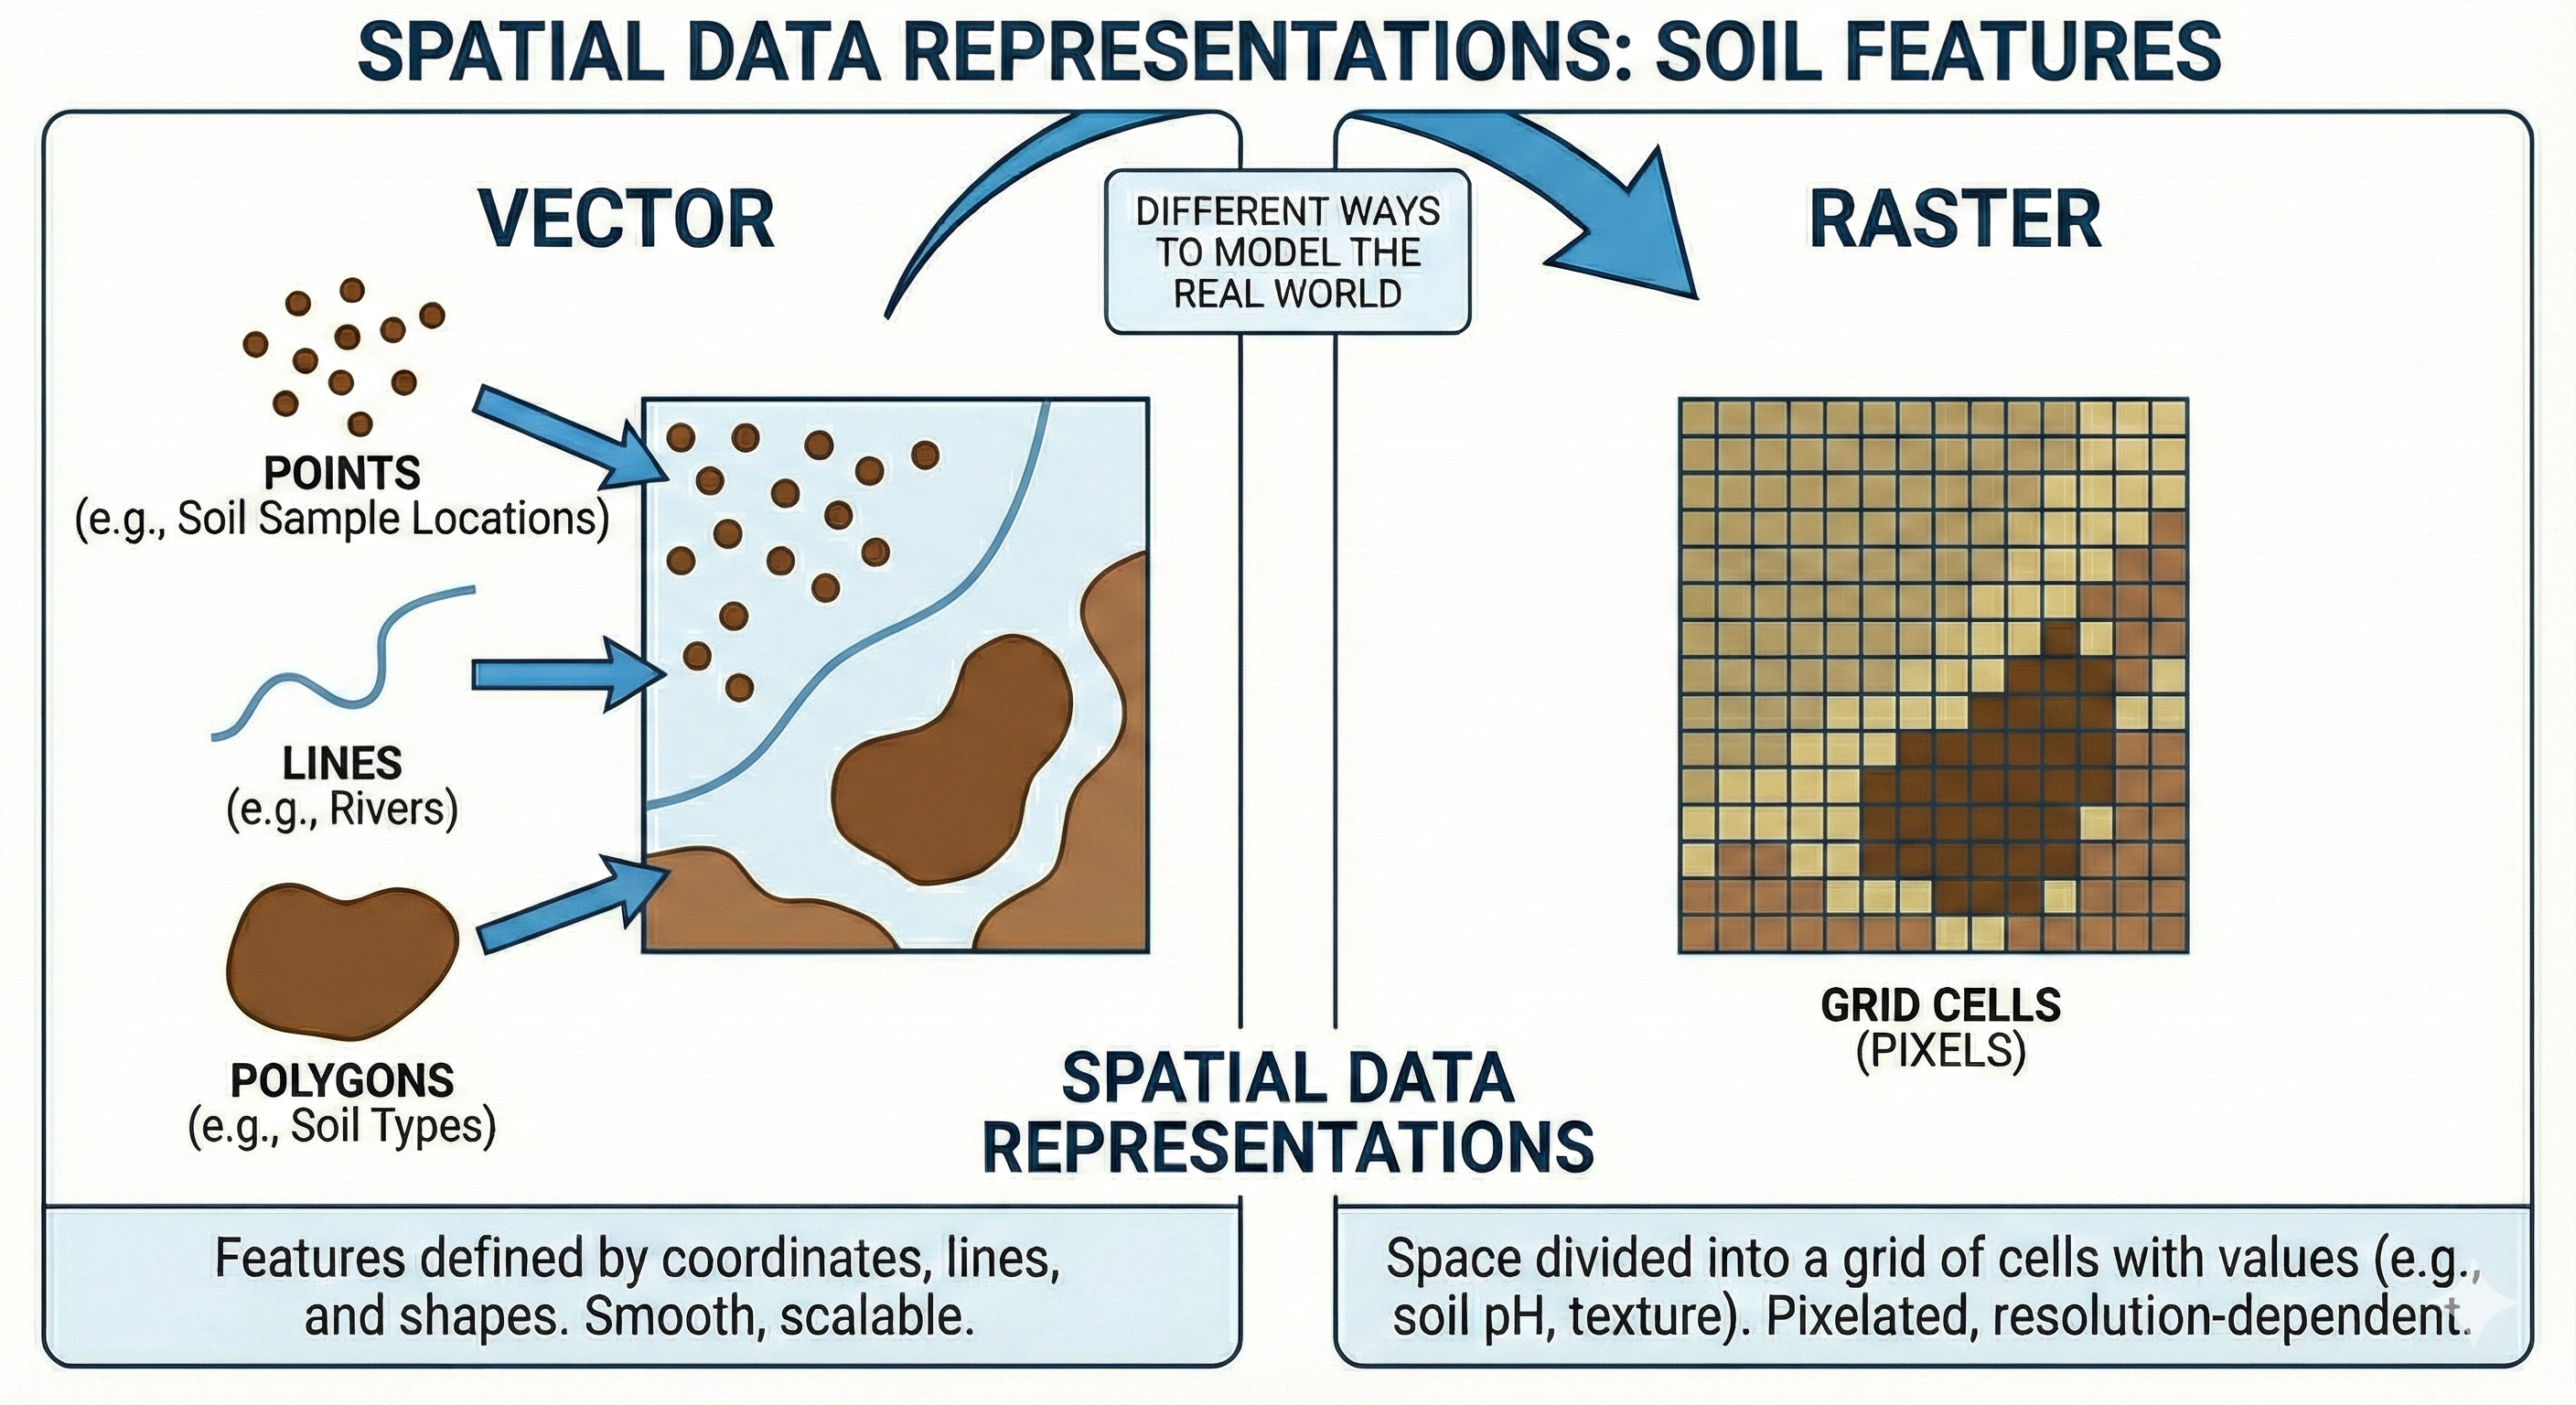
\includegraphics[width=1\linewidth]{images/module1/vectorVSraster} \caption{Vector vs raster data representations}\label{fig:VectRast}
\end{figure}

\textbf{Vector data} represent features as geometries (POINT, LINE, POLYGON) linked to an attribute table. They are ideal for representing discrete spatial objects such as soil sampling points, field boundaries, or landscape units.

\emph{Table 1. Example of layer types and their associated geometry}

\begin{longtable}[]{@{}ll@{}}
\toprule\noalign{}
Layer Type & Geometry \\
\midrule\noalign{}
\endhead
\bottomrule\noalign{}
\endlastfoot
Soil profile locations & POINT \\
Soil sampling locations & POINT \\
Rivers, roads & LINE \\
Fields of sampling plots & POLYGON \\
Farms / Administrative boundaries & POLYGON \\
Land units, physiographic regions & POLYGON \\
\end{longtable}

\textbf{Raster data} represents the landscape as a grid of equal sized cells, each storing a numeric value representing an area defined by the spatial resolution of the raster layer. Raster layers are ideal for continuous spatial phenomena such as soil properties in Digital Soil Mapping.

Examples of raster layers include:

\begin{itemize}
\item
  Digital Elevation Models (DEM)
\item
  Climate variables (rainfall, temperature)
\item
  Remote sensing indices (NDVI, Sentinel-2 bands)
\item
  Soil property predictions (SOC, pH, clay\%)
\item
  Moisture or vegetation products from satellites
\end{itemize}

Both data structures are complementary, and both are required for the creation of digital soil maps.

\subsubsection{Coordinate Reference Systems (CRS) and Projections}\label{coordinate-reference-systems-crs-and-projections}

A Coordinate Reference System (CRS) defines how spatial coordinates relate to positions on Earth. Because Earth is curved, and maps are flat, different CRS systems use different mathematical models to translate the curved space to a planar surface.

The choice of CRS has a major impact on the accuracy of distances, areas, buffer operations, overlays between layers, and spatial modelling outputs.

All spatial objects must include a CRS as part of their metadata. Many common spatial errors come from mixing layers with different or missing CRS.

\paragraph*{Geographic vs projected coordinate systems}\label{geographic-vs-projected-coordinate-systems}
\addcontentsline{toc}{paragraph}{Geographic vs projected coordinate systems}

In Geographic Coordinate Systems (GCS), coordinates are expressed in latitude and longitude with units in \texttt{degrees} (°) (a common example is \texttt{EPSG:4326\ (WGS84)}).

Geographic Coordinate Systems are suitable for storing global data, but they are not appropriate for distance, area, or buffering calculations because degrees are angular units and the ground distance represented by one degree varies with latitude (Fig. \ref{fig:degreeLat}). This variation leads to distortions in distance and area calculations.

\begin{figure}
\includegraphics[width=1\linewidth]{images/module1/degreeEq} \caption{Distance distortion in GCS, where the physical distance of one degree varies by latitude}\label{fig:degreeLat}
\end{figure}

To overcome these limitations, Projected Coordinate Systems (PCS) are designed to reduce distortion over a specific region by transforming the curved surface of the Earth into a flat plane. In a PCS, coordinates are expressed in linear units (usually meters), which makes them suitable for accurate geometric operations such as distance, area, and buffering. Typical examples include UTM zones (e.g., \texttt{EPSG:32614}, \texttt{EPSG:32632}), national grid systems, and local projections optimized for area-specific precision.

To find and compare appropriate CRS options for your data, you can explore available CRS definitions using \href{https://epsg.io/}{https://epsg.io}.

\subsubsection{\texorpdfstring{Spatial Packages in R: \texttt{\{sf\}} and \texttt{\{terra\}}}{Spatial Packages in R: \{sf\} and \{terra\}}}\label{spatial-packages-in-r-sf-and-terra}

\paragraph*{Installing and Loading Spatial Packages}\label{installing-and-loading-spatial-packages}
\addcontentsline{toc}{paragraph}{Installing and Loading Spatial Packages}

\texttt{\{sf\}} and \texttt{\{terra\}} packages are available at CRAN and can be installed using the known \texttt{install.packages()} function.

\begin{Shaded}
\begin{Highlighting}[]
  \FunctionTok{install.packages}\NormalTok{(}\StringTok{"sf"}\NormalTok{)}
  \FunctionTok{install.packages}\NormalTok{(}\StringTok{"terra"}\NormalTok{)}
\end{Highlighting}
\end{Shaded}

Once the packages are installed, you must load them in your R session:

\begin{Shaded}
\begin{Highlighting}[]
  \FunctionTok{library}\NormalTok{(sf)}
  \FunctionTok{library}\NormalTok{(terra)}
\end{Highlighting}
\end{Shaded}

\paragraph*{\texorpdfstring{Working with Vector Data using \texttt{\{sf\}}}{Working with Vector Data using \{sf\}}}\label{working-with-vector-data-using-sf}
\addcontentsline{toc}{paragraph}{Working with Vector Data using \texttt{\{sf\}}}

The \texttt{\{sf\}} package implements the \emph{Simple Features} standard for spatial vector data in R. A \emph{simple feature} is a geometric object (point, line, polygon, etc.) linked to one or more \textbf{attributes} (e.g., soil type, pH, land use).

In practice, an \emph{\texttt{sf} object} is essentially a data frame that includes a geometry column and an associated coordinate system. Thus, it combines:\\

\begin{enumerate}
\def\labelenumi{\arabic{enumi}.}
\tightlist
\item
  \textbf{Attributes} -- ordinary columns (e.g., plot ID, pH, SOC, soil type) just like in a regular data frame.\\
\item
  \textbf{Geometry column} -- typically named \texttt{geom} or \texttt{geometry}, storing coordinates and geometry type.\\
\item
  \textbf{CRS} -- information about the coordinate system used (e.g., WGS84, UTM), as part of the object.\\
\end{enumerate}

\subparagraph*{Importing and Exporting Vector Data}\label{importing-and-exporting-vector-data}
\addcontentsline{toc}{subparagraph}{Importing and Exporting Vector Data}

Vector data represents discrete geographic features such as soil profile locations, field plots, administrative boundaries, roads, or land units.
Vector data is typically stored in formats such as Shapefile, GeoPackage, GeoJSON, or other OGC-compliant files, but can also be stored in plain files with associated coordinates such as \texttt{CSV} files.

\subparagraph*{\texorpdfstring{Creating spatial vector objects from \texttt{CSV} files}{Creating spatial vector objects from CSV files}}\label{creating-spatial-vector-objects-from-csv-files}
\addcontentsline{toc}{subparagraph}{Creating spatial vector objects from \texttt{CSV} files}

Spatial point layers in R can be created directly from regular data frames using the \texttt{\{sf\}} package.
The function \texttt{st\_as\_sf()} converts a data frame into a spatial (vector) object, as long as the data frame contains coordinate columns (e.g., longitude and latitude or projected X/Y coordinates).
To perform this conversion, users must specify the columns containing the coordinates. Even if not mandatory, it is also highly recommended to set the coordinate reference system:

Since importing a \texttt{.csv} file in R typically produces a data frame, the workflow is essentially the same as in the previous example. Once the table is loaded and includes coordinate columns (e.g., X and Y in longitude/latitude), it can be converted to an sf object using \texttt{st\_as\_sf()} by specifying the coordinate columns and the CRS.

\begin{Shaded}
\begin{Highlighting}[]
\CommentTok{\# Import the previously standardized dataset for 0{-}30 cm depth }
\NormalTok{output\_dir }\OtherTok{\textless{}{-}}\StringTok{"03\_outputs/module1/"}
\NormalTok{kdata }\OtherTok{\textless{}{-}} \FunctionTok{read.csv}\NormalTok{ (}\FunctionTok{paste0}\NormalTok{(output\_dir,}\StringTok{"KSSL\_DSM\_0{-}30.csv"}\NormalTok{))}
\CommentTok{\# Convert to sf: create POINT geometry from lon/lat, set CRS = WGS84 (EPSG:4326)}
\NormalTok{soil\_sf }\OtherTok{\textless{}{-}} \FunctionTok{st\_as\_sf}\NormalTok{(kdata, }\AttributeTok{coords =} \FunctionTok{c}\NormalTok{(}\StringTok{"lon"}\NormalTok{, }\StringTok{"lat"}\NormalTok{), }\AttributeTok{crs =} \DecValTok{4326}\NormalTok{)}
\CommentTok{\# Print object geometry}
\NormalTok{soil\_sf}\SpecialCharTok{$}\NormalTok{geometry}
\CommentTok{\# Print CRS details}
\FunctionTok{st\_crs}\NormalTok{(soil\_sf)}
\end{Highlighting}
\end{Shaded}

The Coordinate Reference System (CRS) has been provided as an argument within the \texttt{st\_as\_sf()} function. Users can visualize CRS of sf objects with \texttt{st\_crs()}. the sf object can be transformed to shapefile with \texttt{st\_write}.

\subparagraph*{Exporting sf objects}\label{exporting-sf-objects}
\addcontentsline{toc}{subparagraph}{Exporting sf objects}

Simple features objects can be saved to files or databases using the \texttt{st\_write()} function.

\begin{Shaded}
\begin{Highlighting}[]
\CommentTok{\# Export as shapefile}
\FunctionTok{st\_write}\NormalTok{(soil\_sf, }\FunctionTok{paste0}\NormalTok{(output\_dir,}\StringTok{"soil\_profiles.shp"}\NormalTok{), }\AttributeTok{delete\_layer =} \ConstantTok{TRUE}\NormalTok{) }\CommentTok{\# overwrites shp}
\end{Highlighting}
\end{Shaded}

\subparagraph*{Importing Shapefiles}\label{importing-shapefiles}
\addcontentsline{toc}{subparagraph}{Importing Shapefiles}

Shapefiles can be directly imported into R using the \texttt{st\_read()} function. You can also import most other vector formats with the same command, because \texttt{\{sf\}} automatically detects the file type.

The following chunk imports the soil sampling locations from the cleaned KSSL dataset. This layer represents individual soil pits or auger locations, with coordinates and measured properties stored in the attribute table. The chunk also plots pH values for a quick visual check of the spatial distribution of the data.

\begin{Shaded}
\begin{Highlighting}[]
\CommentTok{\# Read the previously created shapefile containing soil profile points}
\NormalTok{soil\_sf }\OtherTok{\textless{}{-}} \FunctionTok{st\_read}\NormalTok{(}\FunctionTok{paste0}\NormalTok{(output\_dir,}\StringTok{"soil\_profiles.shp"}\NormalTok{))}
\CommentTok{\# Inspect the first rows}
\FunctionTok{head}\NormalTok{(soil\_sf)}
\CommentTok{\# Quick visualization}
\FunctionTok{plot}\NormalTok{(soil\_sf[}\StringTok{"pH"}\NormalTok{], }\AttributeTok{pch =} \DecValTok{16}\NormalTok{, }\AttributeTok{cex =} \FloatTok{0.6}\NormalTok{, }\AttributeTok{key.pos =} \DecValTok{1}\NormalTok{)  }\CommentTok{\# key.pos controls legend position}
\end{Highlighting}
\end{Shaded}

\begin{verbatim}
## Simple feature collection with 6 features and 8 fields
## Geometry type: POINT
## Dimension:     XY
## Bounding box:  xmin: -101.9787 ymin: 38.46796 xmax: -101.7259 ymax: 39.27917
## Geodetic CRS:  WGS 84
##     ProfID top bottom     Clay Silt Sand    SOC   pH                   geometry
## 1 PROF0003   0     30 20.46297 55.9 23.6 1.5744 8.13 POINT (-101.9787 39.06988)
## 2 PROF0004   0     30 22.83169 57.9 19.3 1.3520 6.12 POINT (-101.7832 38.46796)
## 3 PROF0005   0     30 26.41016 58.4 15.2 1.5100 7.25  POINT (-101.7813 38.4703)
## 4 PROF0006   0     30 19.79542 54.9 25.3 1.6500 6.75 POINT (-101.7787 38.47096)
## 5 PROF0007   0     30 25.51856 54.2 20.3 1.6972 7.21  POINT (-101.7467 38.5798)
## 6 PROF0008   0     30 32.35233 57.7  9.9 1.4412 7.84 POINT (-101.7259 39.27917)
\end{verbatim}

\pandocbounded{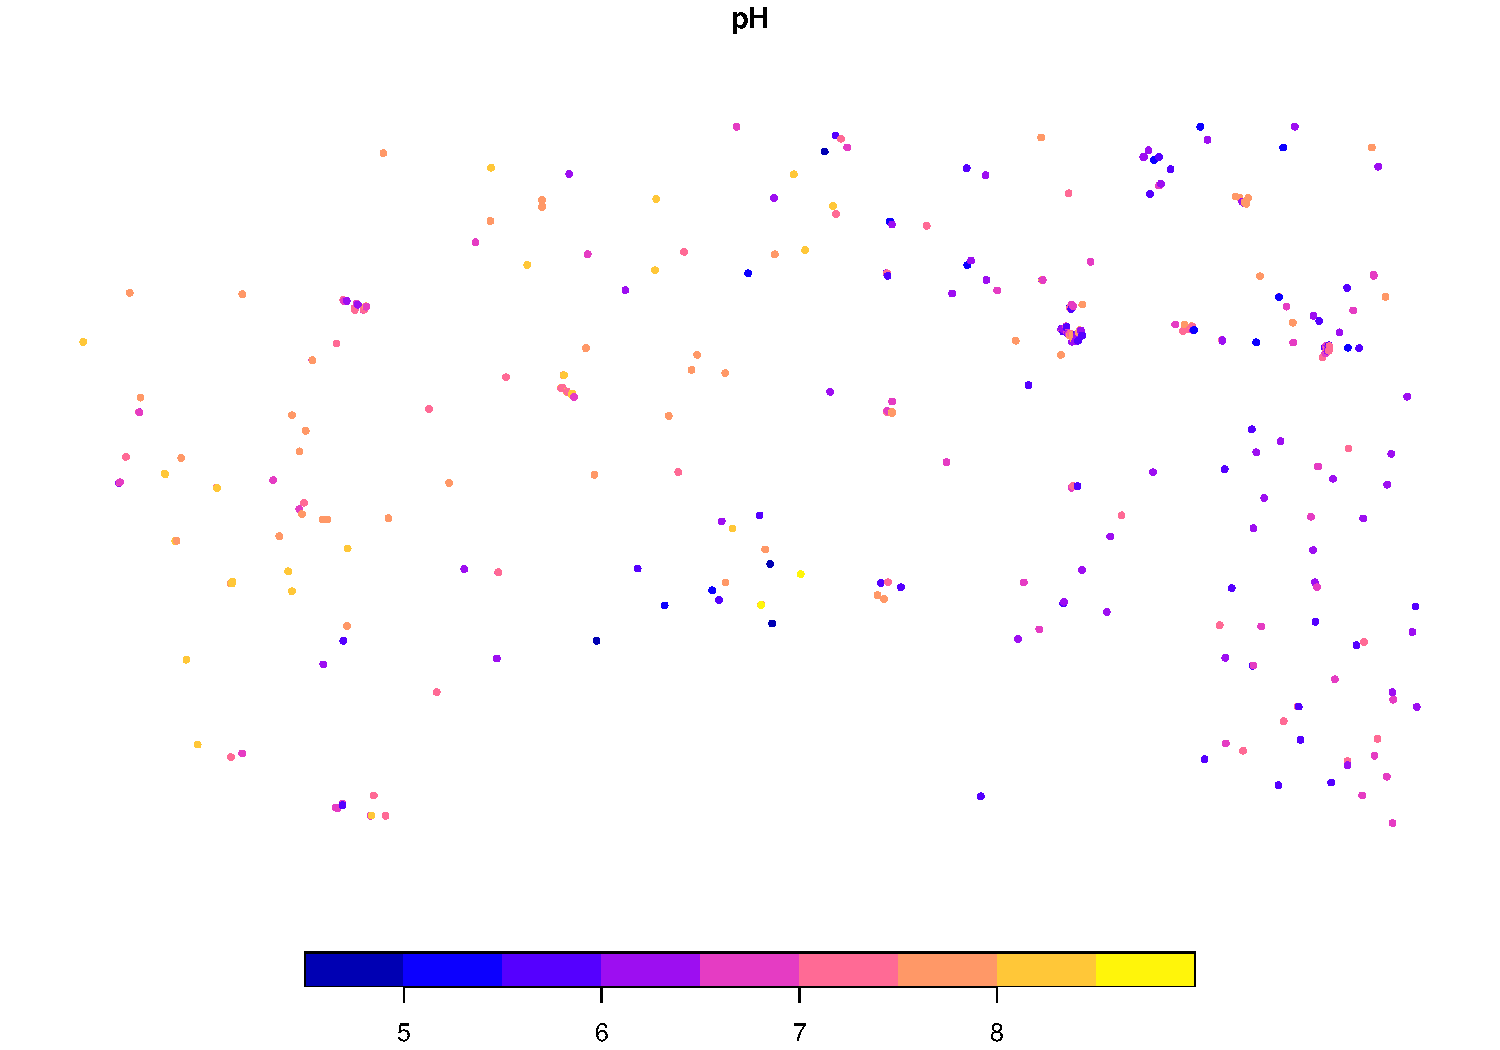
\includegraphics[keepaspectratio]{SoilFER-Integrated-soil-information-for-decision-making_files/SoilFER-Integrated-soil-information-for-decision-making_files/figure-latex/shp-to-sf-hidden-1.pdf}}

\paragraph*{Setting and Reprojecting CRS for vector data}\label{setting-and-reprojecting-crs-for-vector-data}
\addcontentsline{toc}{paragraph}{Setting and Reprojecting CRS for vector data}

It is good practice to always confirm the Coordinate Reference System (CRS) of your spatial data. If the CRS is missing or incorrectly specified, spatial operations such as buffering, distance, and overlay may fail or return misleading results.

As shown previously, the CRS can be defined when creating an sf object (e.g., with \texttt{st\_as\_sf()}). You can inspect the CRS of an \texttt{sf} object with \texttt{st\_crs()}. If the CRS is missing, you can assign it with \texttt{st\_set\_crs()}. To reproject the data into a different CRS (i.e., change the coordinate values to a new reference system), use \texttt{st\_transform()}.

Example: Converting the sf object \texttt{soil\_sf} from Geographic WGS84 (EPSG:4326) to WGS 84 / Pseudo-Mercator (EPSG:3857), a projection commonly used for web mapping.

\begin{Shaded}
\begin{Highlighting}[]
\NormalTok{sf\_3857 }\OtherTok{\textless{}{-}} \FunctionTok{st\_transform}\NormalTok{(soil\_sf, }\DecValTok{3857}\NormalTok{)}

\CommentTok{\# Preview of the projected object}
\FunctionTok{head}\NormalTok{(sf\_3857)}
\end{Highlighting}
\end{Shaded}

\begin{verbatim}
## Simple feature collection with 6 features and 8 fields
## Geometry type: POINT
## Dimension:     XY
## Bounding box:  xmin: -11352220 ymin: 4645745 xmax: -11324070 ymax: 4761739
## Projected CRS: WGS 84 / Pseudo-Mercator
##     ProfID top bottom     Clay Silt Sand    SOC   pH                  geometry
## 1 PROF0003   0     30 20.46297 55.9 23.6 1.5744 8.13 POINT (-11352221 4731687)
## 2 PROF0004   0     30 22.83169 57.9 19.3 1.3520 6.12 POINT (-11330456 4645745)
## 3 PROF0005   0     30 26.41016 58.4 15.2 1.5100 7.25 POINT (-11330245 4646078)
## 4 PROF0006   0     30 19.79542 54.9 25.3 1.6500 6.75 POINT (-11329955 4646172)
## 5 PROF0007   0     30 25.51856 54.2 20.3 1.6972 7.21 POINT (-11326387 4661659)
## 6 PROF0008   0     30 32.35233 57.7  9.9 1.4412 7.84 POINT (-11324071 4761739)
\end{verbatim}

\paragraph*{\texorpdfstring{Inspecting and manipulating \texttt{\{sf\}} Object}{Inspecting and manipulating \{sf\} Object}}\label{inspecting-and-manipulating-sf-object}
\addcontentsline{toc}{paragraph}{Inspecting and manipulating \texttt{\{sf\}} Object}

Because \texttt{sf} objects inherit from the \texttt{data.frame} class, you can explore an sf object with the same tools as data frames (\texttt{class()}, \texttt{str()}, \texttt{summary()}), plus a few \texttt{\{sf\}} helpers (\texttt{st\_geometry\_type()}).

\begin{Shaded}
\begin{Highlighting}[]
\CommentTok{\# Check structure}
\FunctionTok{str}\NormalTok{(soil\_sf)}
\end{Highlighting}
\end{Shaded}

\begin{verbatim}
## Classes 'sf' and 'data.frame':   411 obs. of  9 variables:
##  $ ProfID  : chr  "PROF0003" "PROF0004" "PROF0005" "PROF0006" ...
##  $ top     : int  0 0 0 0 0 0 0 0 0 0 ...
##  $ bottom  : int  30 30 30 30 30 30 30 30 30 30 ...
##  $ Clay    : num  20.5 22.8 26.4 19.8 25.5 ...
##  $ Silt    : num  55.9 57.9 58.4 54.9 54.2 57.7 57.5 63 56.5 59.2 ...
##  $ Sand    : num  23.6 19.3 15.2 25.3 20.3 9.9 8.7 10.5 9.3 5.8 ...
##  $ SOC     : num  1.57 1.35 1.51 1.65 1.7 ...
##  $ pH      : num  8.13 6.12 7.25 6.75 7.21 7.84 7.23 6.2 6.6 7.72 ...
##  $ geometry:sfc_POINT of length 411; first list element:  'XY' num  -102 39.1
##  - attr(*, "sf_column")= chr "geometry"
##  - attr(*, "agr")= Factor w/ 3 levels "constant","aggregate",..: NA NA NA NA NA NA NA NA
##   ..- attr(*, "names")= chr [1:8] "ProfID" "top" "bottom" "Clay" ...
\end{verbatim}

\begin{Shaded}
\begin{Highlighting}[]
\CommentTok{\# Summary of attributes + geometry}
\FunctionTok{summary}\NormalTok{(soil\_sf)}
\end{Highlighting}
\end{Shaded}

\begin{verbatim}
##     ProfID               top        bottom        Clay             Silt      
##  Length:411         Min.   :0   Min.   :30   Min.   : 2.912   Min.   : 3.60  
##  Class :character   1st Qu.:0   1st Qu.:30   1st Qu.:23.081   1st Qu.:48.85  
##  Mode  :character   Median :0   Median :30   Median :29.824   Median :55.80  
##                     Mean   :0   Mean   :30   Mean   :30.146   Mean   :53.24  
##                     3rd Qu.:0   3rd Qu.:30   3rd Qu.:37.148   3rd Qu.:61.80  
##                     Max.   :0   Max.   :30   Max.   :65.460   Max.   :81.40  
##       Sand            SOC              pH                 geometry  
##  Min.   : 0.30   Min.   :0.120   Min.   :4.500   POINT        :411  
##  1st Qu.: 5.00   1st Qu.:1.104   1st Qu.:6.195   epsg:4326    :  0  
##  Median : 9.80   Median :1.600   Median :6.905   +proj=long...:  0  
##  Mean   :16.59   Mean   :1.801   Mean   :6.881                      
##  3rd Qu.:19.30   3rd Qu.:2.268   3rd Qu.:7.660                      
##  Max.   :92.50   Max.   :7.317   Max.   :8.830
\end{verbatim}

\begin{Shaded}
\begin{Highlighting}[]
\CommentTok{\# Check the geometry type. Use head to avoid long printing}
\FunctionTok{head}\NormalTok{(}\FunctionTok{st\_geometry\_type}\NormalTok{(soil\_sf))}
\end{Highlighting}
\end{Shaded}

\begin{verbatim}
## [1] POINT POINT POINT POINT POINT POINT
## 18 Levels: GEOMETRY POINT LINESTRING POLYGON MULTIPOINT ... TRIANGLE
\end{verbatim}

\begin{Shaded}
\begin{Highlighting}[]
\CommentTok{\# Check the CRS:}
\FunctionTok{st\_crs}\NormalTok{(soil\_sf)}
\end{Highlighting}
\end{Shaded}

\begin{verbatim}
## Coordinate Reference System:
##   User input: WGS 84 
##   wkt:
## GEOGCRS["WGS 84",
##     DATUM["World Geodetic System 1984",
##         ELLIPSOID["WGS 84",6378137,298.257223563,
##             LENGTHUNIT["metre",1]]],
##     PRIMEM["Greenwich",0,
##         ANGLEUNIT["degree",0.0174532925199433]],
##     CS[ellipsoidal,2],
##         AXIS["latitude",north,
##             ORDER[1],
##             ANGLEUNIT["degree",0.0174532925199433]],
##         AXIS["longitude",east,
##             ORDER[2],
##             ANGLEUNIT["degree",0.0174532925199433]],
##     ID["EPSG",4326]]
\end{verbatim}

\begin{Shaded}
\begin{Highlighting}[]
\CommentTok{\# Check the spatial extent of the object:}
\FunctionTok{st\_bbox}\NormalTok{(soil\_sf)}
\end{Highlighting}
\end{Shaded}

\begin{verbatim}
##       xmin       ymin       xmax       ymax 
## -101.97873   37.01713  -94.70964   39.98839
\end{verbatim}

\texttt{\{sf\}} objects can be manipulated in the same way as standard data frames while retaining all spatial information.
Base R and \texttt{\{dplyr\}} verbs such as \texttt{filter()}, \texttt{select()}, \texttt{mutate()}, can be directly applied on \texttt{sf} objects.

\begin{Shaded}
\begin{Highlighting}[]
\CommentTok{\# Subset sf rows and columns using the pipping (\%\textgreater{}\%) operator with \{dplyr\}}
\NormalTok{alkaline }\OtherTok{\textless{}{-}}\NormalTok{ soil\_sf }\SpecialCharTok{\%\textgreater{}\%}
  \FunctionTok{filter}\NormalTok{(pH }\SpecialCharTok{\textgreater{}} \FloatTok{7.4}\NormalTok{) }\SpecialCharTok{\%\textgreater{}\%}
  \FunctionTok{select}\NormalTok{(ProfID, pH) }\SpecialCharTok{\%\textgreater{}\%}
  \FunctionTok{mutate}\NormalTok{(}\AttributeTok{alkaline =} \ConstantTok{TRUE}\NormalTok{)}
\CommentTok{\# Preview alkaline data}
\FunctionTok{head}\NormalTok{(alkaline)}
\end{Highlighting}
\end{Shaded}

\begin{verbatim}
## Simple feature collection with 6 features and 3 fields
## Geometry type: POINT
## Dimension:     XY
## Bounding box:  xmin: -101.9787 ymin: 38.50486 xmax: -101.5333 ymax: 39.27917
## Geodetic CRS:  WGS 84
##     ProfID   pH                   geometry alkaline
## 1 PROF0003 8.13 POINT (-101.9787 39.06988)     TRUE
## 2 PROF0008 7.84 POINT (-101.7259 39.27917)     TRUE
## 3 PROF0012 7.72  POINT (-101.667 38.83208)     TRUE
## 4 PROF0013 8.29  POINT (-101.536 38.50828)     TRUE
## 5 PROF0014 8.28  POINT (-101.534 38.50785)     TRUE
## 6 PROF0015 8.29 POINT (-101.5333 38.50486)     TRUE
\end{verbatim}

\paragraph*{Geometry Operations}\label{geometry-operations}
\addcontentsline{toc}{paragraph}{Geometry Operations}

Geometry operations help you \textbf{create new geometries} (e.g., buffers) and \textbf{combine layers} (e.g., clip points to a boundary). In soil science, they are often used to define sampling influence areas, restrict data to an administrative unit, or summarize results by region.

For distance and area-based operations (buffers, distances, areas), work in a Projected CRS (units in metres), not in lon/lat degrees.
Before any geometry operation, make sure both layers are in the same CRS.

\subparagraph*{Buffering Plots (Influence Area)}\label{buffering-plots-influence-area}
\addcontentsline{toc}{subparagraph}{Buffering Plots (Influence Area)}

Buffers are regions created at a fixed distance around geometries (points, lines, or polygons).\\
In soil applications, buffers can represent:

\begin{itemize}
\tightlist
\item
  The influence area of a contaminating facility (polygon geometry).
\item
  Proximity zones around rivers or roads (line geometry).
\item
  Buffer zones around soil sampling points to define their spatial influence (point geometry).
\end{itemize}

The function \texttt{st\_buffer()} is used for this. If the input dataset is in a Geographic Coordinate System (longitude/latitude in degrees), you should first transform it to a Projected Coordinate System (units in metres) before buffering.

\begin{Shaded}
\begin{Highlighting}[]
\CommentTok{\# Original KSSL data is in WGS84 EPSG:4326  geographic coordinates(lon/lat)}
\CommentTok{\# Transform the subset of alkaline soils to NAD83 / UTM 14N (EPSG: 26914)}
\NormalTok{alkaline\_utm }\OtherTok{\textless{}{-}} \FunctionTok{st\_transform}\NormalTok{(alkaline, }\AttributeTok{crs =} \DecValTok{26914}\NormalTok{)  }\CommentTok{\# UTM 14N, distance in metres}

\CommentTok{\# Create a 1 km buffer around each plot}
\NormalTok{plots\_buffer\_1k }\OtherTok{\textless{}{-}} \FunctionTok{st\_buffer}\NormalTok{(alkaline\_utm, }\AttributeTok{dist =} \DecValTok{1000}\NormalTok{)}

\CommentTok{\# Plot buffers (first 3 plots) and then overlay the same points}
\FunctionTok{plot}\NormalTok{(}\FunctionTok{st\_geometry}\NormalTok{(plots\_buffer\_1k[}\DecValTok{1}\SpecialCharTok{:}\DecValTok{3}\NormalTok{, ]), }
     \AttributeTok{col =} \FunctionTok{rgb}\NormalTok{(}\DecValTok{0}\NormalTok{, }\DecValTok{0}\NormalTok{, }\DecValTok{1}\NormalTok{, }\FloatTok{0.3}\NormalTok{), }\AttributeTok{border =} \StringTok{"blue"}\NormalTok{,}
     \AttributeTok{main =} \StringTok{"Plot of first 3 alkaline soils with 1 km buffers"}\NormalTok{)}
\CommentTok{\# Overlay the original sample locations}
\FunctionTok{plot}\NormalTok{(}\FunctionTok{st\_geometry}\NormalTok{(alkaline\_utm[}\DecValTok{1}\SpecialCharTok{:}\DecValTok{3}\NormalTok{, ]), }
     \AttributeTok{add =} \ConstantTok{TRUE}\NormalTok{, }\AttributeTok{pch =} \DecValTok{16}\NormalTok{, }\AttributeTok{col =} \StringTok{"red"}\NormalTok{)}
\end{Highlighting}
\end{Shaded}

\begin{figure}

{\centering 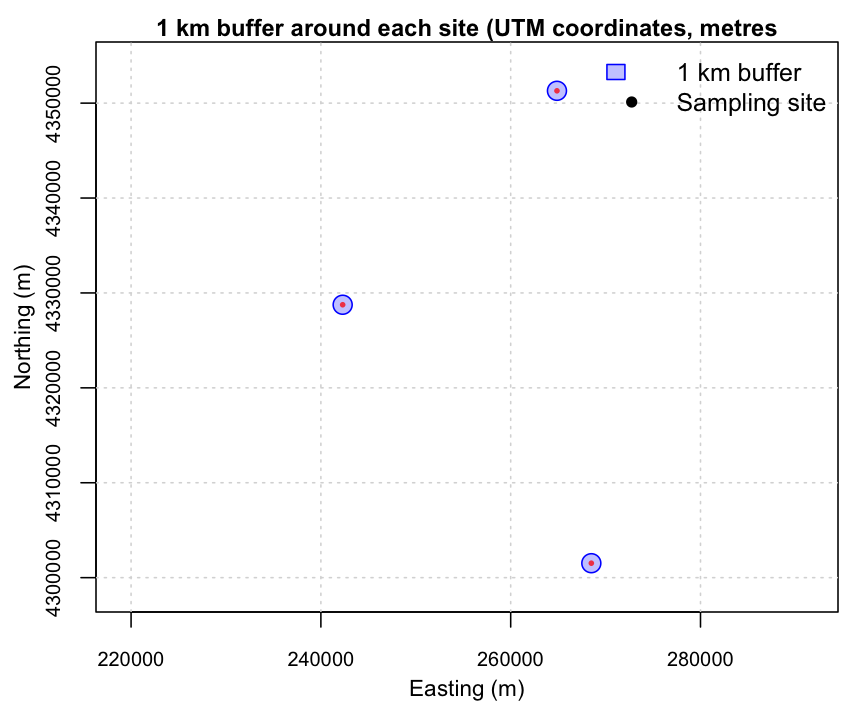
\includegraphics[width=0.7\linewidth]{SoilFER-Training-Resources/01_outputs/buffer_samples} 

}

\caption{1 km buffer around sampling points }\label{fig:unnamed-chunk-1}
\end{figure}

\subparagraph*{Clip Soil Data to Defined Boundaries}\label{clip-soil-data-to-defined-boundaries}
\addcontentsline{toc}{subparagraph}{Clip Soil Data to Defined Boundaries}

In soil data management workflows, it is common to restrict analyses to a defined study area (e.g., a county, district, watershed, or project boundary). This helps ensure that summaries, maps, and models are computed only for the relevant spatial extent.

Two core operations are used repeatedly in Soil Data Management and Digital Soil Mapping:

\begin{itemize}
\item
  \textbf{Clip/subset by boundary} (\texttt{st\_intersection()}): keeps only the features (or parts of features) that fall inside a target boundary.
\item
  \textbf{Dissolve boundaries} (\texttt{st\_union()}): merges multiple polygons into a single boundary by removing internal borders.
\end{itemize}

Use \textbf{clipping} to restrict soil profiles, samples, or observations to a target area before analysis or reporting.

Use \textbf{dissolving} to build a clean study boundary for masking, cropping, mapping, or aggregating results at a higher level.

\textbf{Example 1: Clip sampling points to one administrative unit}

In this example, we clip KSSL sampling points to Riley County. The steps are:

\begin{itemize}
\item
  Read the administrative boundaries layer.
\item
  Transform it to the CRS of the soil points (so layers align).
\item
  Select the target polygon (Riley).
\item
  Clip the soil points to that polygon.
\end{itemize}

\begin{Shaded}
\begin{Highlighting}[]
\CommentTok{\# Read administrative boundaries (example file)}
\NormalTok{admin }\OtherTok{\textless{}{-}} \FunctionTok{st\_read}\NormalTok{(}\StringTok{"01\_data/module1/shapes/Tiger\_2020\_Counties.shp"}\NormalTok{)}
\CommentTok{\# Ensure both layers share the same CRS}
\NormalTok{admin }\OtherTok{\textless{}{-}} \FunctionTok{st\_transform}\NormalTok{(admin, }\FunctionTok{st\_crs}\NormalTok{(soil\_sf))}
\CommentTok{\# Example: select one unit (replace with your column/value)}
\NormalTok{study\_area }\OtherTok{\textless{}{-}}\NormalTok{ admin[admin}\SpecialCharTok{$}\NormalTok{NAME }\SpecialCharTok{==} \StringTok{"Riley"}\NormalTok{, ]}
\CommentTok{\# Keep only points inside the study area}
\NormalTok{soil\_clip }\OtherTok{\textless{}{-}} \FunctionTok{st\_intersection}\NormalTok{(soil\_sf, study\_area)}
\CommentTok{\# Plot result}
\FunctionTok{plot}\NormalTok{(}\FunctionTok{st\_geometry}\NormalTok{(study\_area), }\AttributeTok{col =} \ConstantTok{NA}\NormalTok{, }\AttributeTok{border =} \StringTok{"black"}\NormalTok{, }\AttributeTok{main=}\StringTok{"Sampled soils in Riley County"}\NormalTok{, }\AttributeTok{cex.main =} \DecValTok{1}\NormalTok{ )}
\FunctionTok{plot}\NormalTok{(}\FunctionTok{st\_geometry}\NormalTok{(soil\_clip), }\AttributeTok{add =} \ConstantTok{TRUE}\NormalTok{, }\AttributeTok{pch =} \DecValTok{16}\NormalTok{, }\AttributeTok{col =} \StringTok{"red"}\NormalTok{, }\AttributeTok{cex =} \FloatTok{0.6}\NormalTok{)}
\end{Highlighting}
\end{Shaded}

\begin{figure}

{\centering 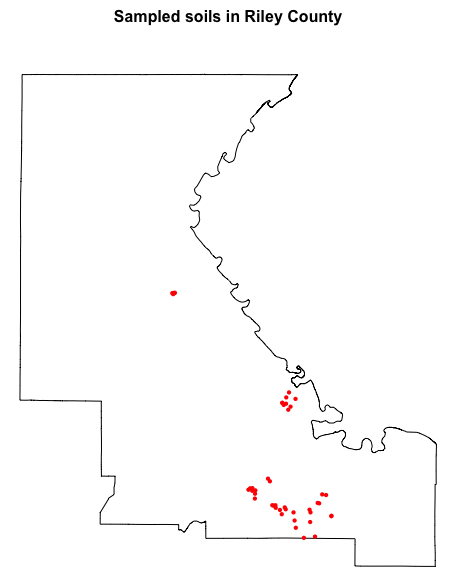
\includegraphics[width=0.5\linewidth]{SoilFER-Training-Resources/01_outputs/riley_samples} 

}

\caption{Sampled soils in Riley County}\label{fig:unnamed-chunk-2}
\end{figure}

In this case, \texttt{soil\_clip} preserves all attributes from the original sampling dataset (\texttt{soil\_sf}) and includes the attributes of the administrative polygon \texttt{admin} at each point.

\textbf{Example 2: Dissolve polygons to create a single study region boundary}

Dissolving is useful when you want a single boundary for a larger study region. For example, you may want to combine all counties into a single Kansas state outline (or merge multiple polygons representing a project area).

\texttt{st\_union()} merges all polygons into one geometry and removes internal borders.

\begin{Shaded}
\begin{Highlighting}[]
\CommentTok{\# Dissolve all counties into one Kansas boundary}
\NormalTok{admin\_dissolved }\OtherTok{\textless{}{-}} \FunctionTok{st\_union}\NormalTok{(admin)}
\CommentTok{\# Plot comparison: before vs after dissolve}
\CommentTok{\# Adjust graphics settings to 1 row x 2 columns layout with tight margins}
\NormalTok{op }\OtherTok{\textless{}{-}} \FunctionTok{par}\NormalTok{(}
  \AttributeTok{mfrow =} \FunctionTok{c}\NormalTok{(}\DecValTok{1}\NormalTok{, }\DecValTok{2}\NormalTok{),}
  \AttributeTok{mar =} \FunctionTok{c}\NormalTok{(}\FloatTok{0.5}\NormalTok{, }\FloatTok{0.5}\NormalTok{, }\FloatTok{0.1}\NormalTok{, }\FloatTok{0.5}\NormalTok{),  }\CommentTok{\# very small top margin}
  \AttributeTok{xaxs =} \StringTok{"i"}\NormalTok{, }\AttributeTok{yaxs =} \StringTok{"i"}
\NormalTok{)}
\FunctionTok{plot}\NormalTok{(}\FunctionTok{st\_geometry}\NormalTok{(admin[}\DecValTok{1}\NormalTok{]),}
     \AttributeTok{col =} \ConstantTok{NA}\NormalTok{, }\AttributeTok{border =} \StringTok{"black"}\NormalTok{,}
     \AttributeTok{axes =} \ConstantTok{FALSE}\NormalTok{, }\AttributeTok{asp =} \DecValTok{1}\NormalTok{)}
\FunctionTok{title}\NormalTok{(}\StringTok{"Before dissolve"}\NormalTok{, }\AttributeTok{line =} \SpecialCharTok{{-}}\FloatTok{0.6}\NormalTok{, }\AttributeTok{cex.main =} \FloatTok{0.95}\NormalTok{)}
\FunctionTok{plot}\NormalTok{(}\FunctionTok{st\_geometry}\NormalTok{(admin\_dissolved),}
     \AttributeTok{col =} \ConstantTok{NA}\NormalTok{, }\AttributeTok{border =} \StringTok{"black"}\NormalTok{,}
     \AttributeTok{axes =} \ConstantTok{FALSE}\NormalTok{, }\AttributeTok{asp =} \DecValTok{1}\NormalTok{)}
\FunctionTok{title}\NormalTok{(}\StringTok{"After dissolve"}\NormalTok{, }\AttributeTok{line =} \SpecialCharTok{{-}}\FloatTok{0.6}\NormalTok{, }\AttributeTok{cex.main =} \FloatTok{0.95}\NormalTok{)}
\CommentTok{\# restore graphics settings}
\FunctionTok{par}\NormalTok{(op)}
\end{Highlighting}
\end{Shaded}

\begin{figure}
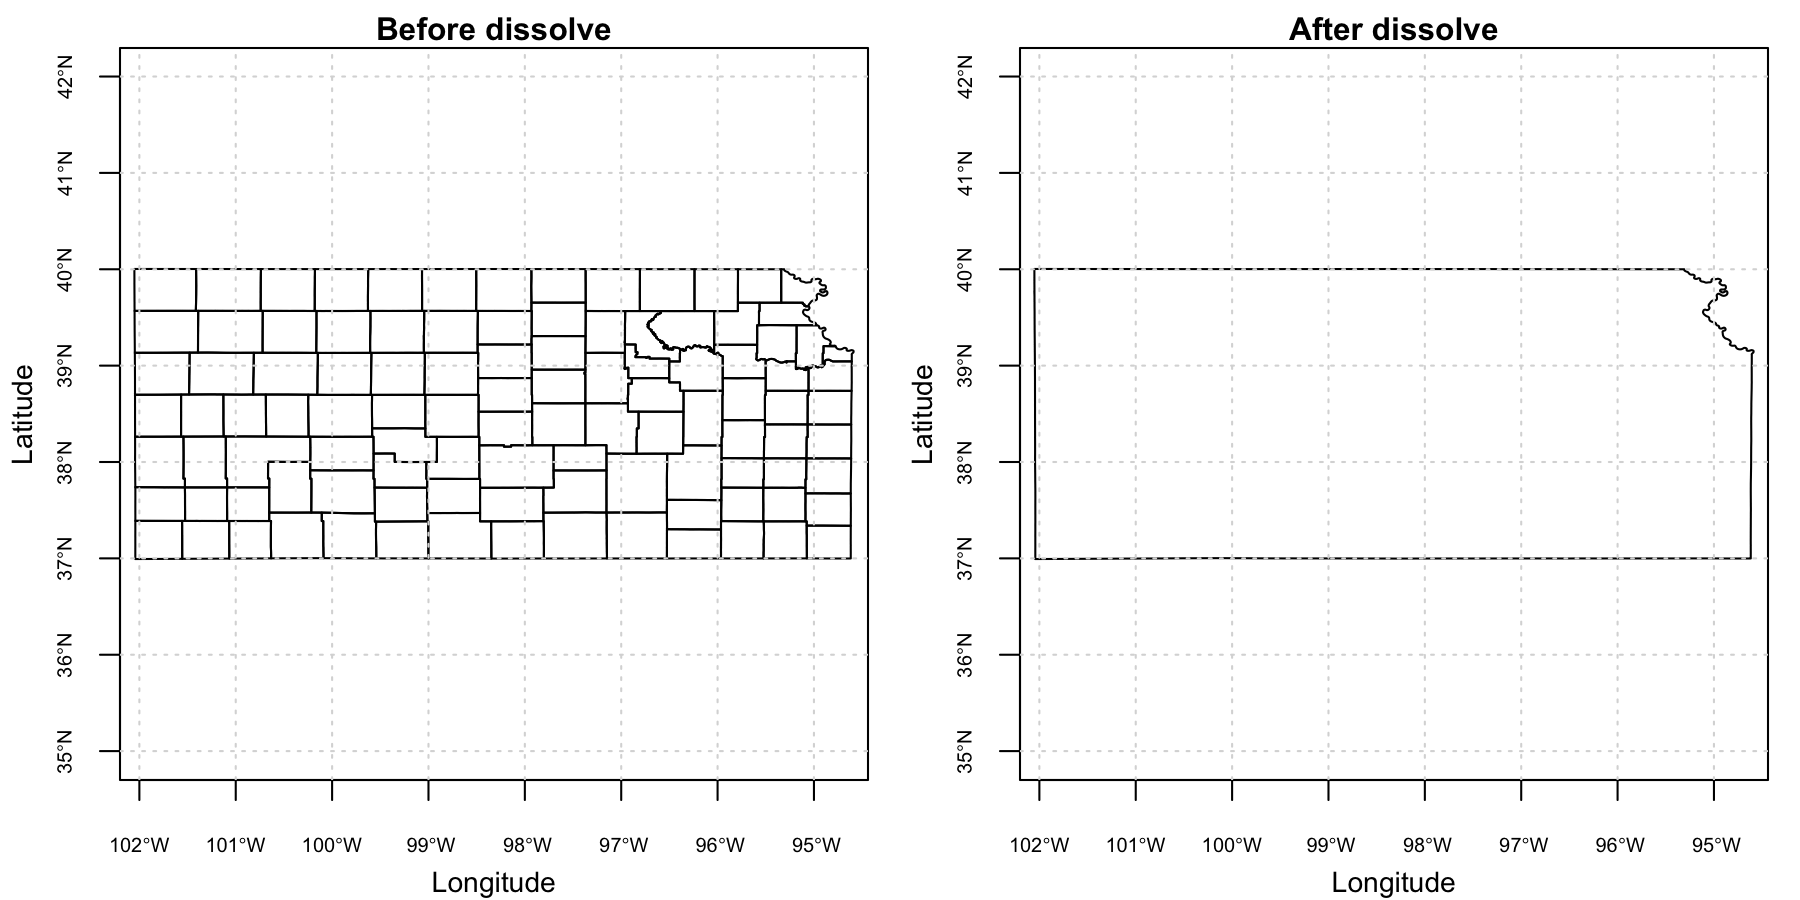
\includegraphics[width=1\linewidth]{SoilFER-Training-Resources/01_outputs/dissolve_before_after} \caption{Dissolving polygons on Kansas County vector data}\label{fig:unnamed-chunk-3}
\end{figure}

\subparagraph*{Spatial Relationships and Joins}\label{spatial-relationships-and-joins}
\addcontentsline{toc}{subparagraph}{Spatial Relationships and Joins}

Spatial relationships help answer questions about how spatial features relate to one another (e.g., whether a point falls inside a polygon, or how far two features are apart).

\textbf{Spatial predicates} (return TRUE/FALSE relationships):

\begin{itemize}
\item
  \texttt{st\_intersects()} (touch/overlap)
\item
  \texttt{st\_within()} (inside)
\item
  \texttt{st\_distance()} (distance between features)
\end{itemize}

\textbf{Spatial joins} attach attributes from one layer to another:

\begin{itemize}
\tightlist
\item
  \texttt{st\_join()} (e.g., assign each soil profile to an administrative unit)
\end{itemize}

Example: assign each sampling point to an administrative polygon.

\begin{Shaded}
\begin{Highlighting}[]
\CommentTok{\# Ensure both layers share the same CRS}
\NormalTok{alkaline }\OtherTok{\textless{}{-}} \FunctionTok{st\_transform}\NormalTok{(alkaline, }\FunctionTok{st\_crs}\NormalTok{(admin))}
\CommentTok{\# Join admin attributes to points (points inherit polygon attributes)}
\NormalTok{alkaline\_with\_admin }\OtherTok{\textless{}{-}} \FunctionTok{st\_join}\NormalTok{(alkaline, admin, }\AttributeTok{join =}\NormalTok{ st\_within)}
\CommentTok{\# Preview result}
\FunctionTok{head}\NormalTok{(alkaline\_with\_admin)}
\end{Highlighting}
\end{Shaded}

\begin{verbatim}
## Simple feature collection with 6 features and 20 fields
## Geometry type: POINT
## Dimension:     XY
## Bounding box:  xmin: -101.9787 ymin: 38.50486 xmax: -101.5333 ymax: 39.27917
## Geodetic CRS:  WGS 84
##     ProfID   pH alkaline STATEFP COUNTYFP COUNTYNS GEOID    NAME       NAMELSAD
## 1 PROF0003 8.13     TRUE      20      199 00485060 20199 Wallace Wallace County
## 2 PROF0008 7.84     TRUE      20      181 00485053 20181 Sherman Sherman County
## 3 PROF0012 7.72     TRUE      20      199 00485060 20199 Wallace Wallace County
## 4 PROF0013 8.29     TRUE      20      203 00485062 20203 Wichita Wichita County
## 5 PROF0014 8.28     TRUE      20      203 00485062 20203 Wichita Wichita County
## 6 PROF0015 8.29     TRUE      20      203 00485062 20203 Wichita Wichita County
##   LSAD CLASSFP MTFCC CSAFP CBSAFP METDIVFP FUNCSTAT AWATER    INTPTLAT
## 1   06      H1 G4020  <NA>   <NA>     <NA>        A 140936 +38.9266259
## 2   06      H1 G4020  <NA>   <NA>     <NA>        A 548248 +39.3513521
## 3   06      H1 G4020  <NA>   <NA>     <NA>        A 140936 +38.9266259
## 4   06      H1 G4020  <NA>   <NA>     <NA>        A  61987 +38.4819222
## 5   06      H1 G4020  <NA>   <NA>     <NA>        A  61987 +38.4819222
## 6   06      H1 G4020  <NA>   <NA>     <NA>        A  61987 +38.4819222
##       INTPTLON                             GlobalID                   geometry
## 1 -101.7711031 5d2c40a3-7c2d-4f48-879b-11e53b1bc366 POINT (-101.9787 39.06988)
## 2 -101.7198590 111d187f-9907-4a48-8678-a1bed6840eb9 POINT (-101.7259 39.27917)
## 3 -101.7711031 5d2c40a3-7c2d-4f48-879b-11e53b1bc366  POINT (-101.667 38.83208)
## 4 -101.3474341 c1ad0367-fe83-4ee2-91fb-256e33e36857  POINT (-101.536 38.50828)
## 5 -101.3474341 c1ad0367-fe83-4ee2-91fb-256e33e36857  POINT (-101.534 38.50785)
## 6 -101.3474341 c1ad0367-fe83-4ee2-91fb-256e33e36857 POINT (-101.5333 38.50486)
\end{verbatim}

\paragraph*{\texorpdfstring{Visualizing \texttt{\{sf\}} Objects}{Visualizing \{sf\} Objects}}\label{visualizing-sf-objects}
\addcontentsline{toc}{paragraph}{Visualizing \texttt{\{sf\}} Objects}

As shown previously, \texttt{\{sf\}} objects can be quickly visualized using the base R \texttt{plot()} function. This is convenient for fast checks (e.g., verifying geometry and extent), but it offers limited control over plot appearance and legend design.

In contrast, \texttt{\{ggplot2\}} provides a consistent \emph{`grammar of graphics'} that makes it easier to produce publication-ready maps. Key benefits include:

\begin{itemize}
\item
  Full control of aesthetics (colors, symbol size, line width, transparency) and clear legends.
\item
  High-quality themes and consistent styling across figures (useful in reports and publications).
\item
  Easy layering of multiple spatial objects (points, polygons, buffers, rasters---when combined with other tools).
\item
  Faceting to compare maps by groups (e.g., land use class, sampling campaign, depth interval).
\end{itemize}

In \texttt{\{ggplot2\}}, spatial geometries are plotted with \texttt{geom\_sf().}

\begin{Shaded}
\begin{Highlighting}[]
\FunctionTok{library}\NormalTok{(ggplot2)}
\FunctionTok{ggplot}\NormalTok{(}\AttributeTok{data =}\NormalTok{ soil\_sf) }\SpecialCharTok{+}
  \FunctionTok{geom\_sf}\NormalTok{(}\FunctionTok{aes}\NormalTok{(}\AttributeTok{color =}\NormalTok{ pH), }\AttributeTok{size =} \DecValTok{2}\NormalTok{) }\SpecialCharTok{+}
  \FunctionTok{scale\_color\_viridis\_c}\NormalTok{() }\SpecialCharTok{+}
  \FunctionTok{theme\_minimal}\NormalTok{() }\SpecialCharTok{+}
  \FunctionTok{labs}\NormalTok{(}
    \AttributeTok{title =} \StringTok{"Soil sampling sites – pH"}\NormalTok{,}
    \AttributeTok{color =} \StringTok{"pH"}
\NormalTok{  )}
\end{Highlighting}
\end{Shaded}

\begin{figure}
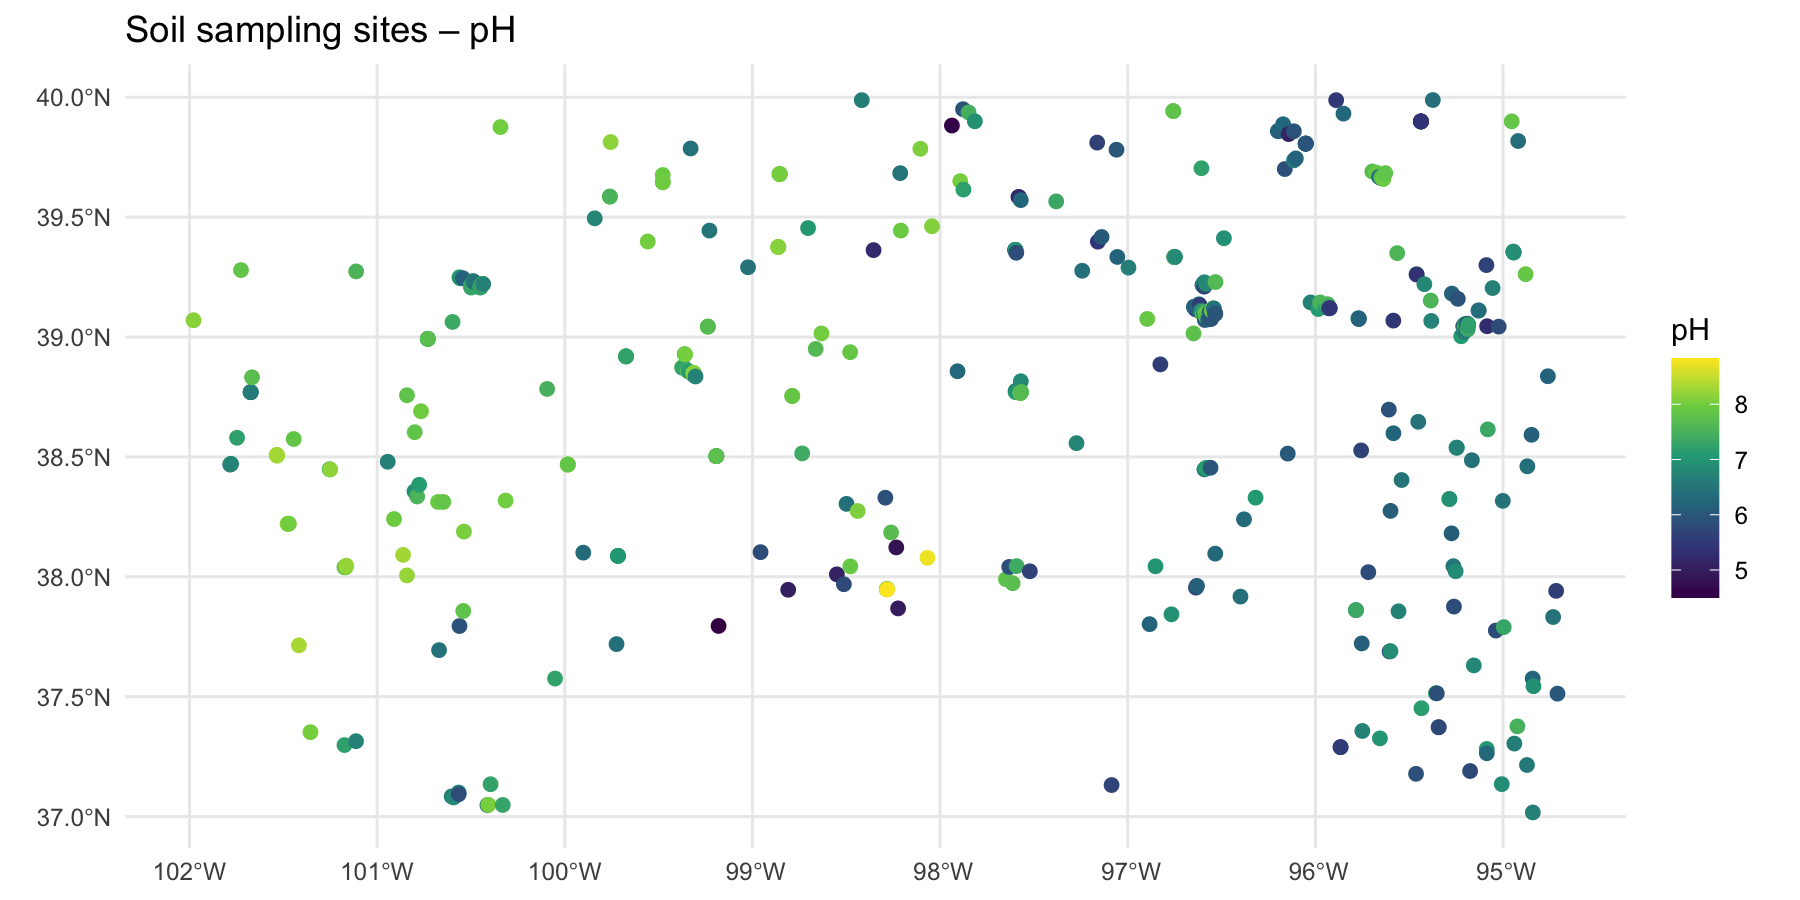
\includegraphics[width=1\linewidth]{SoilFER-Training-Resources/01_outputs/ggplot_ph} \caption{Visualization of pH values with ggplot2}\label{fig:unnamed-chunk-4}
\end{figure}

The possibilities for visualization with \texttt{\{ggplot2\}} are extensive. For more examples and options, see the \texttt{\{ggplot2\}} documentation and the \texttt{\{sf\}} vignettes on plotting with \texttt{geom\_sf()}.

\begin{center}\rule{0.5\linewidth}{0.5pt}\end{center}

\subsection{Preparing Raster Covariates}\label{preparing-raster-covariates}

The workflows presented in this tutorial use environmental covariates as proxies to describe the spatial variation of soil properties. These covariates support two key steps:

\begin{itemize}
\item
  \textbf{Sampling design}: covariates are used to identify environmental clusters that should be sampled, helping maximize the representation of soil variability while optimizing sampling effort.
\item
  \textbf{Digital Soil Mapping (DSM)}: soil properties measured at known point locations (vector data) are related to environmental characteristics (raster covariates) to train statistical or machine learning models that predict soil properties continuously across space.The foundations of DSM were defined by the \emph{scorpan} framework, which transforms explanatory factors of soil genesis to provide an empirical predictive tool for spatial mapping (further explained in \hyperref[SCORPAN-Framework]{The SCORPAN Framework})
\end{itemize}

The preparation of covariates is a time-consuming task. Therefore, this tutorial uses a pre-compiled set of environmental covariates to fulfil these tasks. It assembles five categories of environmental covariates cloud-optimized GeoTIFF files.

\textbf{Climate data} is sourced from two complementary products.

\begin{itemize}
\item
  \textbf{CHELSA} (Climatologies at High resolution for the Earth's Land Surface Areas) provides long-term bioclimatic variables including mean annual temperature (bio1), annual precipitation (bio12), and extreme temperature and precipitation metrics (bio5, bio6, bio13, bio14, bio16, bio17), alongside potential evapotranspiration computed using the Penman-Monteith method and surface wind statistics.
\item
  \textbf{TerraClimate} contributes monthly time series of maximum and minimum temperature, precipitation, and potential evapotranspiration spanning 1981 to the present, which are exported as multi-band images for subsequent temporal aggregation in R.
\end{itemize}

\textbf{Terrain data} is derived from the USGS SRTM 30 m Digital Elevation Model, from which slope, aspect, Topographic Position Index (TPI), and hillshade are computed on-the-fly within GEE. Geomorphological landform classification at 90 m resolution is obtained from the \texttt{Geomorpho90m} dataset. Additionally, pre-computed terrain derivatives at 250 m resolution (elevation, slope, curvature, TPI, TWI) are loaded from the FAO GSP shared GEE asset library hosted at \texttt{projects/digital-soil-mapping-gsp-fao}.

\textbf{Vegetation and soil indices} are computed from Sentinel-2 Surface Reflectance imagery (Copernicus/S2\_SR\_HARMONIZED), filtered to scenes with less than 10\% cloud cover and cloud-masked using the QA60 quality band. The script computes the Normalized Difference Vegetation Index (NDVI), Enhanced Vegetation Index (EVI), Normalized Difference Bareness and Soil Index (NDBSI), Redness Index, Brightness Index, NBR+, and the Visible-Near-Short-wave Infrared Index (VNSIR). Seasonal vegetation dynamics are additionally captured through MODIS FPAR mean and standard deviation layers for four three-month periods covering the full annual cycle.

\textbf{Soil Available Water Content} represents the mean available water capacity (AWC - in mm) of soil from 0 to 200 cm depth.

\textbf{Land cover} is represented by the ESA WorldCover 2021 product at 10 m resolution, from which a cropland mask is derived by isolating the cropland class (value 40) for use in masking or stratified analyses.

\begin{quote}
Note: users need to have a google account to access the covariate data.
\end{quote}

\paragraph*{Download Covariate Rasters}\label{download-covariate-rasters}
\addcontentsline{toc}{paragraph}{Download Covariate Rasters}

A dedicated Google Drive folder has been created to store large raster files used in this tutorial. Users can obtain the data directly from the folder \texttt{rasters} following link:
\url{https://drive.google.com/drive/folders/1K7tq9zX5HsqbqWcNoT27WtfPtehcKBCu}

Data in this folder includes:

\begin{itemize}
\tightlist
\item
  \href{https://drive.google.com/file/d/1wh6xSW03YKrCHScJJa0c_cSA1XZ8tYY-/view?usp=drive_link}{\textbf{Cropland\_Mask\_KANSAS.tif}} (22.5 mb): Binary raster with presence (1) and absence (NA) of crops in Kansas at 20-meter resolution. This file is used as a mask to avoid non-cropped areas in the analyses.
\item
  \href{https://drive.google.com/file/d/1wURPmPLi2LdYq6zBhZN1e91EiiZsk8oX/view?usp=drive_link}{\textbf{Environmental\_Covariates\_250m\_KANSAS.tif}} (203.2 mb): Multi-layer raster stack with climatic, remote sensing, topographic information at 250-meter resolution.
\item
  \href{https://drive.google.com/file/d/1xf89gn4pBKsb5ynVIfKZd4MbT3ZL1Nf2/view?usp=drive_link}{\textbf{HighRes\_Covariates\_100m\_Kansas.tif}} (535.6 mb). 100-meter resolution rasters with remote sensing derived information.
\item
  \href{https://drive.google.com/file/d/14KmmjjTfVD7jTEuQqCLkfcQmXy0VBDkA/view?usp=drive_link}{\textbf{DEM\_KANSAS.tif}} (21.4 mb). 100-meter resolution rasters with remote sensing derived information.
\item
  \href{https://drive.google.com/file/d/1rESziVFlEvEEmrKacb88R1pKZxbrU7qS/view?usp=drive_link}{\textbf{Slope\_KANSAS.tif}} (61.2 mb). 100-meter resolution rasters with remote sensing derived information.
\item
  {[}\textbf{Geomorphon\_Landforms\_KANSAS}{]}(\citeproc{ref-amatulli2020_geomorpho90m}{Amatulli \emph{et al.}, 2020})(\url{https://drive.google.com/file/d/1E03U42UPl9SKMfUGZZ8qDCno2H_kPxUB/view?usp=drive_link}) (14.9 mb). 90-meter resolution raster of geomorphological types from Geomorpho90m -- Global High-Resolution Geomorphometry Layers.
\item
  \href{https://drive.google.com/file/d/1TyyErHkQeNW9Q_wchW9Fa_0UpdaWS_-_/view?usp=drive_link}{\textbf{TerraClimate\_AvgTemp\_1981\_2023\_KANSAS.tif}} (17.7 mb). 100 m TerraClimate monthly averaged Temperature rasters from 1981-2023.
\item
  \href{https://drive.google.com/file/d/1b9wM3zwggBFS98pFEyWUFtpKN9ORq9we/view?usp=drive_link}{\textbf{TerraClimate\_PET\_1981\_2023\_KANSAS.tif}} (17.2 mb). 100 m TerraClimate monthly averaged Potential Evapotranspiration rasters from 1981-2023.
\item
  \href{https://drive.google.com/file/d/1xq6y8jNUjDbipXHQE1w67f_vxQeXACkH/view?usp=drive_link}{\textbf{TerraClimate\_Precip\_1981\_2023\_KANSAS.tif}} (11.9 mb). 100 m TerraClimate monthly accumulated mean Precipitation rasters from 1981-2023.
\item
  {[}\textbf{sol\_available.water.capacity\_usda.mm\_m\_250m\_0..200cm\_1950..2017\_v0.1.tif}{]}(\citeproc{ref-gupta_zenodo_2019}{Gupta and Hengl, 2019})(\url{https://drive.google.com/file/d/1nG0yCr-tNPzeeEvzcGrtdQxRHnQ6NMH5/view?usp=drive_link}). 250-meter resolution geospatial raster dataset representing the mean available water capacity (AWC - in mm) of soil from 0 to 200 cm depth.
\item
  {[}\textbf{ESA\_WorldCover\_2021\_KANSAS}{]}(\citeproc{ref-zanaga2022_worldcover2021_v200}{Zanaga \emph{et al.}, 2022})(\url{https://drive.google.com/file/d/1xq6y8jNUjDbipXHQE1w67f_vxQeXACkH/view?usp=drive_link}) (11.9 mb). 10-meter resolution rasters of landcover types from the European Space Agency WorldCover, based on Sentinel-1 and Sentinel-2 data.
\end{itemize}

\emph{Table. ESA WorldCover (global land cover) legend, the class codes and color in the Map band.}

\begin{longtable}[]{@{}rll@{}}
\toprule\noalign{}
Value & Class & Color (hex) \\
\midrule\noalign{}
\endhead
\bottomrule\noalign{}
\endlastfoot
10 & Tree cover & \texttt{\#006400} \\
20 & Shrubland & \texttt{\#ffbb22} \\
30 & Grassland & \texttt{\#ffff4c} \\
40 & Cropland & \texttt{\#f096ff} \\
50 & Built-up & \texttt{\#fa0000} \\
60 & Bare / sparse vegetation & \texttt{\#b4b4b4} \\
70 & Snow and ice & \texttt{\#f0f0f0} \\
80 & Permanent water bodies & \texttt{\#0064c8} \\
90 & Herbaceous wetland & \texttt{\#0096a0} \\
95 & Mangroves & \texttt{\#00cf75} \\
100 & Moss and lichen & \texttt{\#fae6a0} \\
\end{longtable}

\paragraph*{Obtain Covariate Data from Google Earth Engine (GEE)}\label{obtain-covariate-data-from-google-earth-engine-gee}
\addcontentsline{toc}{paragraph}{Obtain Covariate Data from Google Earth Engine (GEE)}

The data can also be generated directly using Google Earth Engine (GEE). GEE provides direct access to many environmental datasets through a unified interface, allowing analysts to extract, compute, and export ready-to-use covariate stacks for any region of interest using a single script.

The script provided with this training (\texttt{02\_scripts/module1/1\_gee\_soilfer\_env\_covariates.txt}) contains step-by-step instructions to download the covariate data from the GEE platform.

The data has already been processed for this training and is available to download from this \href{https://drive.google.com/drive/folders/1EGrkhbMTi2qglemuD_onegAqLWZb3BbT}{link}. Place these files into the \texttt{training\_data} folder within \texttt{01\_data/module1} and set the path for the covariate rasters and spectral data:

\begin{Shaded}
\begin{Highlighting}[]
\CommentTok{\# Define the relative path to the folder with the downloaded covariates}
\CommentTok{\# }\AlertTok{NOTE}\CommentTok{: Adapt this path to your project structure}
\NormalTok{  training\_dir }\OtherTok{\textless{}{-}}\StringTok{"01\_data/module1/training\_data"}
\end{Highlighting}
\end{Shaded}

\paragraph*{Running the GEE Script}\label{running-the-gee-script}
\addcontentsline{toc}{paragraph}{Running the GEE Script}

Copy the full contents of \texttt{1\_gee\_soilfer\_env\_covariates.txt} into the GEE Code Editor. Before running, review and adjust the configuration variables at the top of the script (Section 1) to match your study area and requirements.

The \texttt{aoi} variable defines the \texttt{area\ of\ interest}. For the training exercise, this is already configured to use the US Census TIGER state boundary layer:

\begin{Shaded}
\begin{Highlighting}[]
\KeywordTok{var}\NormalTok{ aoi }\OperatorTok{=}\NormalTok{ ee}\OperatorTok{.}\FunctionTok{FeatureCollection}\NormalTok{(}\StringTok{\textquotesingle{}TIGER/2018/States\textquotesingle{}}\NormalTok{)}
  \OperatorTok{.}\FunctionTok{filter}\NormalTok{(ee}\OperatorTok{.}\AttributeTok{Filter}\OperatorTok{.}\FunctionTok{eq}\NormalTok{(}\StringTok{\textquotesingle{}NAME\textquotesingle{}}\OperatorTok{,} \StringTok{\textquotesingle{}Kansas\textquotesingle{}}\NormalTok{))}\OperatorTok{;}
\end{Highlighting}
\end{Shaded}

To adapt the script to a different study area, replace this definition with a custom geometry or a different administrative boundary. Update \texttt{countryName} to a short descriptor used in the exported file names.

The date range for TerraClimate is controlled by \texttt{climateStartDate} and \texttt{climateEndDate}. The default configuration covers the full 1981--2023 record. For exploratory or training purposes, restricting this range (e.g., 2000--2023) reduces processing time and export file sizes.

Export spatial resolutions are defined individually for each product category, reflecting the native resolution of each data source: 250 m for the primary CHELSA/MODIS covariate stack, 100 m for high-resolution terrain and Sentinel-2 layers, 90 m for geomorphons, 20 m for the cropland mask, and 4000 m for TerraClimate time series.

Click \textbf{Run} to execute the script. Visualization layers (SRTM DEM, Sentinel-2 RGB composite, and cropland mask) will appear on the map immediately. Export tasks do not start automatically --- navigate to the \textbf{Tasks} tab in the right panel and click \textbf{Run} next to each pending task to initiate the exports to Google Drive.

\textbf{Processing Time and Quotas}

Large exports, particularly \textbf{TerraClimate} time series and \textbf{Sentinel-2} layers over large regions, can take tens of minutes to several hours depending on server load and area size. GEE free-tier accounts are subject to computation quotas. If a task fails with a computation timeout or memory error, consider reducing the export resolution or splitting the time series into shorter periods. Monitor task progress in the \textbf{Tasks} tab; completed files will appear in your \texttt{GEE\_Exports} Google Drive folder once finished.

Once all exports are complete, download the GeoTIFF files from Google Drive to your local working directory. In subsequent modules, these rasters will be loaded into R using the \texttt{terra} package and stacked into the covariate array used in the next modules.

\subsubsection{\texorpdfstring{Working with Raster Data using \texttt{\{terra\}}}{Working with Raster Data using \{terra\}}}\label{working-with-raster-data-using-terra}

The \texttt{\{terra\}} package is the main framework for working with raster spatial data in R. A raster represents space as a regular grid of cells, where each cell stores a value (e.g., elevation, land cover class, rainfall, SOC prediction). Raster layers are widely used in Digital Soil Mapping both as covariates (environmental predictors) and as model outputs (predicted soil properties).

In practice, a \texttt{terra::SpatRaster} object combines:

\begin{itemize}
\item
  Cell values: the data stored in the grid cells (continuous values like temperature, or categorical values like land cover).
\item
  Spatial geometry: the grid definition given by the extent (spatial coverage) and resolution (cell size).
\item
  CRS: the coordinate reference system used (e.g., WGS84, UTM).
\item
  Layers: a raster can have one layer (e.g., DEM, SOC) or multiple layers (a covariate stack).
\end{itemize}

\paragraph*{Importing and Exporting Raster Data}\label{importing-and-exporting-raster-data}
\addcontentsline{toc}{paragraph}{Importing and Exporting Raster Data}

Raster files are commonly distributed as GeoTIFFs (.tif). The function \texttt{rast()} reads both single-layer and multi-layer rasters. Rasters can be exported back to disk with \texttt{writeRaster()}.

\begin{Shaded}
\begin{Highlighting}[]
\FunctionTok{library}\NormalTok{(terra)}
\CommentTok{\# Read a single{-}layer raster (e.g., cropland mask or DEM)}
\NormalTok{crops }\OtherTok{\textless{}{-}} \FunctionTok{rast}\NormalTok{(}\FunctionTok{paste0}\NormalTok{(training\_dir,}\StringTok{"Cropland\_Mask\_KANSAS.tif"}\NormalTok{))}
\CommentTok{\# Read a multi{-}layer raster (e.g., environmental covariates stack)}
\NormalTok{covs }\OtherTok{\textless{}{-}} \FunctionTok{rast}\NormalTok{(}\FunctionTok{paste0}\NormalTok{(training\_dir,}\StringTok{"Environmental\_Covariates\_250m\_KANSAS.tif"}\NormalTok{))}
\end{Highlighting}
\end{Shaded}

To save raster data to disk use \texttt{writeRaster}:

\begin{Shaded}
\begin{Highlighting}[]
\CommentTok{\# Export a raster as GeoTIFF}
\FunctionTok{writeRaster}\NormalTok{(crops, }\StringTok{"03\_outputs/module1/Cropland\_Mask\_KANSAS.tif"}\NormalTok{, }\AttributeTok{overwrite =} \ConstantTok{TRUE}\NormalTok{) }\CommentTok{\# overwrites tif}
\end{Highlighting}
\end{Shaded}

\paragraph*{\texorpdfstring{Inspecting and Exploring \texttt{SpatRaster} Objects}{Inspecting and Exploring SpatRaster Objects}}\label{inspecting-and-exploring-spatraster-objects}
\addcontentsline{toc}{paragraph}{Inspecting and Exploring \texttt{SpatRaster} Objects}

Before analysis, inspect the spatial properties (extent, resolution, CRS), the number of layers, and the value ranges. This helps detect common issues such as mismatched CRS, unexpected resolution, incorrect extents, or missing data patterns.

\begin{Shaded}
\begin{Highlighting}[]
\CommentTok{\# Basic metadata (prints summary to console)}
\NormalTok{covs}
\CommentTok{\# Number of layers}
\FunctionTok{nlyr}\NormalTok{(covs)}
\CommentTok{\# Spatial properties}
\FunctionTok{ext}\NormalTok{(covs)}
\FunctionTok{res}\NormalTok{(covs)}
\FunctionTok{crs}\NormalTok{(covs)}
\CommentTok{\# Layer names (multi{-}layer rasters)}
\FunctionTok{names}\NormalTok{(covs)}
\CommentTok{\# Value ranges for the first 4 layers}
\FunctionTok{global}\NormalTok{(covs[[}\DecValTok{1}\SpecialCharTok{:}\DecValTok{4}\NormalTok{]], }\AttributeTok{fun =} \StringTok{"range"}\NormalTok{, }\AttributeTok{na.rm =} \ConstantTok{TRUE}\NormalTok{)}
\CommentTok{\# Histograms of the first 4 layers}
\CommentTok{\# Adjust graphics settings to 2 row x 2 columns layout with tight margins}
\NormalTok{op }\OtherTok{\textless{}{-}} \FunctionTok{par}\NormalTok{(}
  \AttributeTok{mfrow =} \FunctionTok{c}\NormalTok{(}\DecValTok{2}\NormalTok{, }\DecValTok{2}\NormalTok{),}
  \AttributeTok{mar  =} \FunctionTok{c}\NormalTok{(}\FloatTok{3.5}\NormalTok{, }\FloatTok{3.5}\NormalTok{, }\FloatTok{2.2}\NormalTok{, }\FloatTok{1.2}\NormalTok{),  }\CommentTok{\# more space around each panel}
  \AttributeTok{oma  =} \FunctionTok{c}\NormalTok{(}\DecValTok{1}\NormalTok{, }\DecValTok{1}\NormalTok{, }\DecValTok{1}\NormalTok{, }\DecValTok{1}\NormalTok{),          }\CommentTok{\# extra space around the whole figure}
  \AttributeTok{mgp  =} \FunctionTok{c}\NormalTok{(}\FloatTok{2.2}\NormalTok{, }\FloatTok{0.7}\NormalTok{, }\DecValTok{0}\NormalTok{)          }\CommentTok{\# axis title/labels spacing}
\NormalTok{)}

\ControlFlowTok{for}\NormalTok{ (i }\ControlFlowTok{in} \DecValTok{1}\SpecialCharTok{:}\DecValTok{4}\NormalTok{) \{}
  \FunctionTok{hist}\NormalTok{(covs[[i]],}
       \AttributeTok{main =} \FunctionTok{paste}\NormalTok{(}\StringTok{"Histogram of"}\NormalTok{, }\FunctionTok{names}\NormalTok{(covs)[i]),}
       \AttributeTok{xlab =} \FunctionTok{names}\NormalTok{(covs)[i])}
\NormalTok{\}}
\CommentTok{\# restore previous graphics settings}
\FunctionTok{par}\NormalTok{(op)}
\end{Highlighting}
\end{Shaded}

\begin{figure}
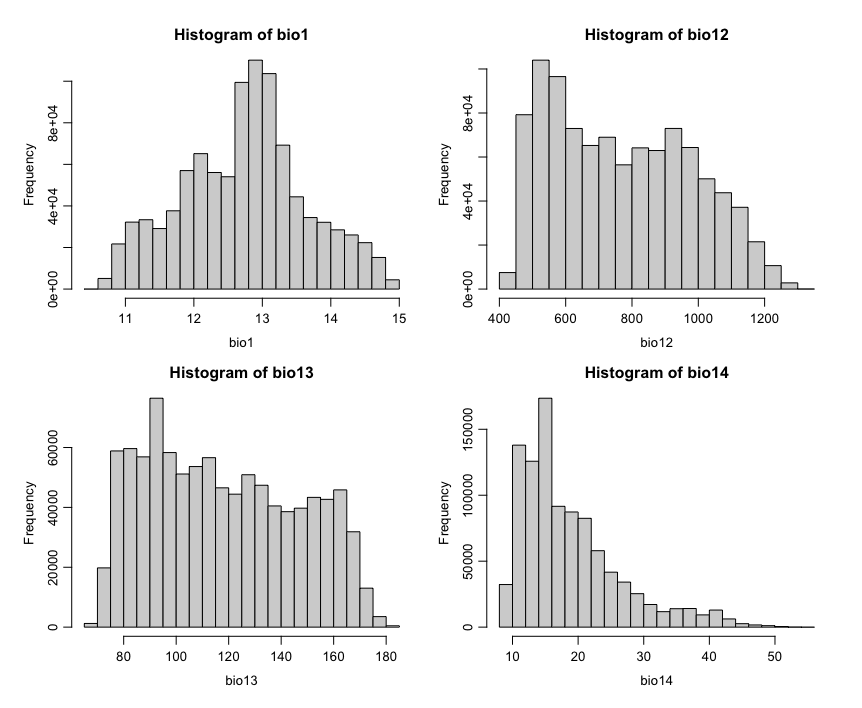
\includegraphics[width=1\linewidth]{SoilFER-Training-Resources/01_outputs/hist_covs} \caption{Visualization of histograms of covariates}\label{fig:unnamed-chunk-5}
\end{figure}

For most raster operations, rasters should share the same CRS, resolution, and extent. If they do not, they typically need adjustment using functions such as \texttt{project()}, \texttt{resample()}, and \texttt{crop()} before combining.

\paragraph*{Raster Visualization}\label{raster-visualization}
\addcontentsline{toc}{paragraph}{Raster Visualization}

Rasters can be quickly visualized using \texttt{plot()}. For multi-layer rasters, it is common to plot a subset of layers.

\begin{Shaded}
\begin{Highlighting}[]
\CommentTok{\# Plot single{-}layer crops raster mask}
\FunctionTok{plot}\NormalTok{(crops, }\AttributeTok{main=}\StringTok{"Cropland Mask"}\NormalTok{)}
\end{Highlighting}
\end{Shaded}

\begin{figure}
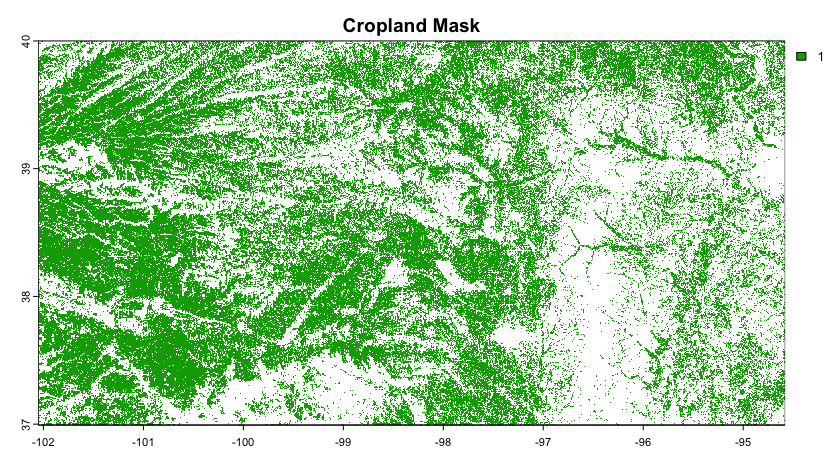
\includegraphics[width=1\linewidth]{SoilFER-Training-Resources/01_outputs/plot_crops} \caption{Visualization of raster crop mask}\label{fig:unnamed-chunk-6}
\end{figure}

\begin{Shaded}
\begin{Highlighting}[]
\CommentTok{\# Plot a multi{-}layer raster (e.g., environmental covariates stack)}
\FunctionTok{plot}\NormalTok{(covs)}
\end{Highlighting}
\end{Shaded}

\begin{figure}
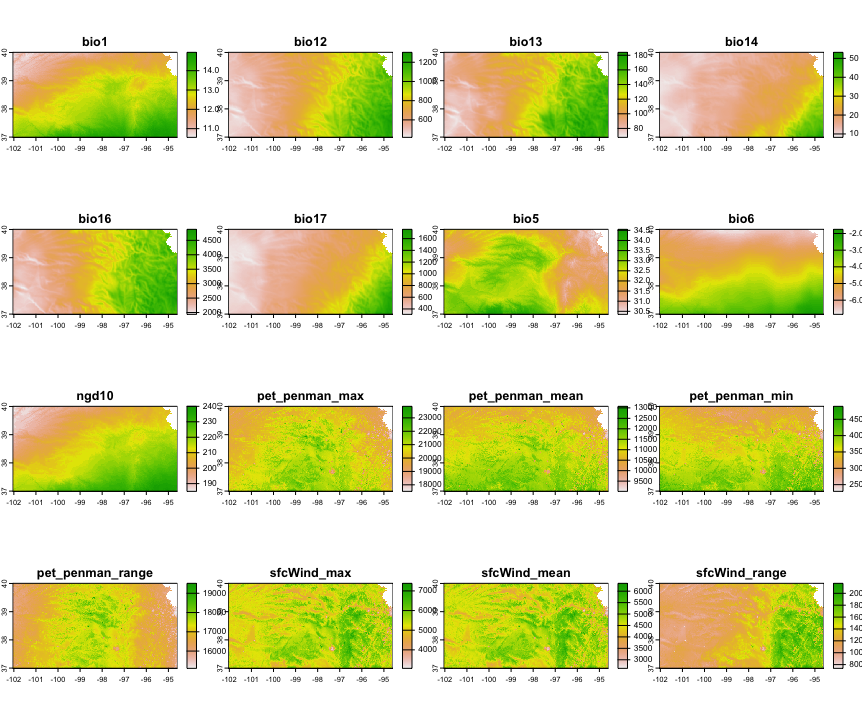
\includegraphics[width=1\linewidth]{SoilFER-Training-Resources/01_outputs/plot_covs} \caption{Visualization of covariates}\label{fig:unnamed-chunk-7}
\end{figure}

You can also plot specific layers by name:

\begin{Shaded}
\begin{Highlighting}[]
\CommentTok{\# Plot Elevation and Temperature from the covs stack}
\CommentTok{\# Adjust graphics settings to 1 row x 2 columns layout with tight margins}
\NormalTok{op }\OtherTok{\textless{}{-}} \FunctionTok{par}\NormalTok{(}
  \AttributeTok{mfrow =} \FunctionTok{c}\NormalTok{(}\DecValTok{1}\NormalTok{, }\DecValTok{2}\NormalTok{),}
  \AttributeTok{mar =} \FunctionTok{c}\NormalTok{(}\FloatTok{0.5}\NormalTok{, }\FloatTok{0.5}\NormalTok{, }\FloatTok{0.5}\NormalTok{, }\FloatTok{0.5}\NormalTok{),}
  \AttributeTok{xaxs =} \StringTok{"i"}\NormalTok{, }\AttributeTok{yaxs =} \StringTok{"i"}
\NormalTok{)}
\FunctionTok{plot}\NormalTok{(covs[[}\StringTok{"dtm\_elevation\_250m"}\NormalTok{]], }\AttributeTok{main =} \StringTok{"Elevation (DEM)"}\NormalTok{, }\AttributeTok{cex.main =}\NormalTok{ .}\DecValTok{8}\NormalTok{)}
\FunctionTok{plot}\NormalTok{(covs[[}\StringTok{"bio1"}\NormalTok{]], }\AttributeTok{main =} \StringTok{"Annual Mean Temperature"}\NormalTok{, }\AttributeTok{cex.main =}\NormalTok{ .}\DecValTok{8}\NormalTok{)}
\FunctionTok{par}\NormalTok{(op) }\CommentTok{\# restore previous graphics settings}
\end{Highlighting}
\end{Shaded}

\begin{figure}
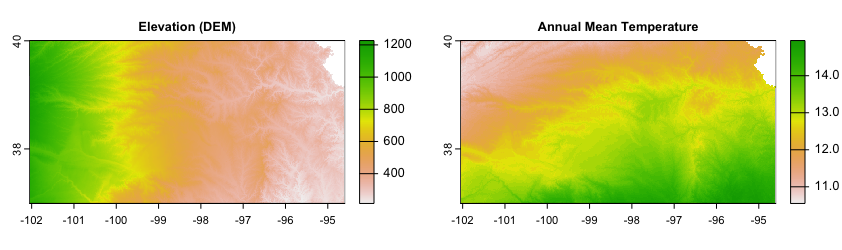
\includegraphics[width=1\linewidth]{SoilFER-Training-Resources/01_outputs/plot_E_T} \caption{Visualization of Elevation and Temperature}\label{fig:unnamed-chunk-8}
\end{figure}

\paragraph*{Setting and Reprojecting CRS for Raster Data}\label{setting-and-reprojecting-crs-for-raster-data}
\addcontentsline{toc}{paragraph}{Setting and Reprojecting CRS for Raster Data}

Rasters also have a CRS. You can inspect it with \texttt{crs()}. To reproject a raster to a new CRS, use \texttt{project()}. Reprojection may change the grid and requires interpolation (resampling), so it is more computationally intensive than vector reprojection.

\begin{Shaded}
\begin{Highlighting}[]
\CommentTok{\# Inspect CRS}
\FunctionTok{crs}\NormalTok{(covs)}
\CommentTok{\# Reproject raster (example: to EPSG:3857)}
\NormalTok{covs\_3857 }\OtherTok{\textless{}{-}} \FunctionTok{project}\NormalTok{(covs, }\StringTok{"EPSG:3857"}\NormalTok{)}
\end{Highlighting}
\end{Shaded}

\paragraph*{Spatial Operations on Rasters}\label{spatial-operations-on-rasters}
\addcontentsline{toc}{paragraph}{Spatial Operations on Rasters}

Raster operations are used to prepare consistent covariate stacks, restrict layers to a study area, and combine tiled outputs.

\subparagraph*{Merge rasters (mosaic)}\label{merge-rasters-mosaic}
\addcontentsline{toc}{subparagraph}{Merge rasters (mosaic)}

Adjacent raster tiles can be merged into a single, continuous layer using \texttt{mosaic()}. This is common when rasters are exported as tiles (e.g., from Google Earth Engine). In the example below, two binary cropland mask tiles are mosaicked and written as a compact GeoTIFF.

\begin{Shaded}
\begin{Highlighting}[]
\CommentTok{\# Read input rasters (adjacent tiles)}
\NormalTok{r1 }\OtherTok{\textless{}{-}} \FunctionTok{rast}\NormalTok{(}\FunctionTok{paste0}\NormalTok{(training\_dir,}\StringTok{"Cropland\_Mask\_KANSAS{-}0000000000{-}0000000000.tif"}\NormalTok{))}
\NormalTok{r2 }\OtherTok{\textless{}{-}} \FunctionTok{rast}\NormalTok{(}\FunctionTok{paste0}\NormalTok{(training\_dir,}\StringTok{"Cropland\_Mask\_KANSAS{-}0000000000{-}0000023296.tif"}\NormalTok{))}
\CommentTok{\# Mosaic into a single raster}
\NormalTok{m }\OtherTok{\textless{}{-}} \FunctionTok{mosaic}\NormalTok{(r1, r2, }\AttributeTok{fun =} \StringTok{"max"}\NormalTok{)}
\CommentTok{\# Cast to integer to optimize file size (not valid for non{-}integer continuous data)}
\NormalTok{m }\OtherTok{\textless{}{-}} \FunctionTok{as.int}\NormalTok{(m)}
\CommentTok{\# Write output with compression to reduce file size}
\FunctionTok{writeRaster}\NormalTok{(m,}\StringTok{"03\_outputs/module1/Cropland\_Mask\_KANSAS.tif"}\NormalTok{, }\AttributeTok{overwrite =} \ConstantTok{TRUE}\NormalTok{,}
  \AttributeTok{wopt =} \FunctionTok{list}\NormalTok{(}\AttributeTok{datatype =} \StringTok{"INT1U"}\NormalTok{,  }\CommentTok{\# Byte (0–255); NA retained as NoData}
    \AttributeTok{gdal =} \FunctionTok{c}\NormalTok{(}\StringTok{"COMPRESS=DEFLATE"}\NormalTok{, }\StringTok{"PREDICTOR=2"}\NormalTok{, }\StringTok{"ZLEVEL=9"}\NormalTok{, }\StringTok{"TILED=YES"}\NormalTok{)}
\NormalTok{  )}
\NormalTok{)}
\end{Highlighting}
\end{Shaded}

\subparagraph*{\texorpdfstring{Crop and mask to study area (\texttt{crop()}, \texttt{mask()})}{Crop and mask to study area (crop(), mask())}}\label{crop-and-mask-to-study-area-crop-mask}
\addcontentsline{toc}{subparagraph}{Crop and mask to study area (\texttt{crop()}, \texttt{mask()})}

Use \texttt{crop()} to reduce the raster extent, and \texttt{mask()} to set values outside the boundary to NA.

\begin{Shaded}
\begin{Highlighting}[]
\CommentTok{\# Crop and mask covariates to the extent of Riley}
\CommentTok{\# Align CRS of both datasets}
\NormalTok{admin }\OtherTok{\textless{}{-}} \FunctionTok{st\_transform}\NormalTok{(admin, }\FunctionTok{crs}\NormalTok{(covs))}
\CommentTok{\# Crop covariates to the extent of the county}
\NormalTok{covs\_crop }\OtherTok{\textless{}{-}} \FunctionTok{crop}\NormalTok{(covs, admin[admin}\SpecialCharTok{$}\NormalTok{NAME}\SpecialCharTok{==}\StringTok{"Riley"}\NormalTok{,])}
\CommentTok{\# Mask covariates}
\NormalTok{covs\_mask }\OtherTok{\textless{}{-}} \FunctionTok{mask}\NormalTok{(covs\_crop, admin[admin}\SpecialCharTok{$}\NormalTok{NAME}\SpecialCharTok{==}\StringTok{"Riley"}\NormalTok{,])}

\CommentTok{\# Plot covariate (bio1 = temperature) in Riley County}
\CommentTok{\# Adjust graphics settings to 1 row x 2 columns layout with tight margins}
\NormalTok{op }\OtherTok{\textless{}{-}} \FunctionTok{par}\NormalTok{(}
  \AttributeTok{mfrow =} \FunctionTok{c}\NormalTok{(}\DecValTok{1}\NormalTok{, }\DecValTok{2}\NormalTok{),}
  \AttributeTok{mar =} \FunctionTok{c}\NormalTok{(}\FloatTok{0.5}\NormalTok{, }\FloatTok{0.5}\NormalTok{, }\FloatTok{0.5}\NormalTok{, }\FloatTok{0.5}\NormalTok{),}
  \AttributeTok{xaxs =} \StringTok{"i"}\NormalTok{, }\AttributeTok{yaxs =} \StringTok{"i"}
\NormalTok{)}
\FunctionTok{plot}\NormalTok{(covs\_crop[[}\StringTok{"bio1"}\NormalTok{]], }\AttributeTok{main=} \StringTok{"Crop"}\NormalTok{, }\AttributeTok{cex.main =} \DecValTok{1}\NormalTok{)}
\FunctionTok{plot}\NormalTok{(covs\_mask[[}\StringTok{"bio1"}\NormalTok{]], }\AttributeTok{main=} \StringTok{"Mask"}\NormalTok{, }\AttributeTok{cex.main =} \DecValTok{1}\NormalTok{)}
\CommentTok{\# restore previous graphics settings}
\FunctionTok{par}\NormalTok{(op) }
\end{Highlighting}
\end{Shaded}

\begin{figure}
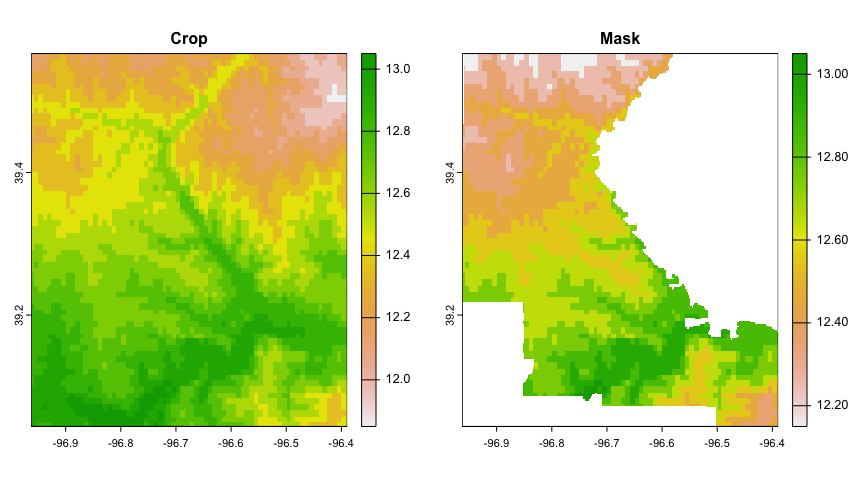
\includegraphics[width=0.8\linewidth]{SoilFER-Training-Resources/01_outputs/crop_riley} \caption{Differences of Crop and Mask outputs in raster data}\label{fig:unnamed-chunk-9}
\end{figure}

\textbf{\texttt{crop()} and \texttt{mask()} are complementary operations.}

\begin{itemize}
\item
  \texttt{crop()} reduces a raster to the extent of a vector polygon (it keeps all cells within the polygon's bounding box), while \texttt{mask()} retains only the cells inside the polygon and sets values outside to \texttt{NA}.
\item
  If you want to limit a raster to a specific boundary and keep only the data within that area, first apply \texttt{crop()} and then \texttt{mask()}.
\end{itemize}

\subparagraph*{\texorpdfstring{Resampling and alignment (\texttt{resample()})}{Resampling and alignment (resample())}}\label{resampling-and-alignment-resample}
\addcontentsline{toc}{subparagraph}{Resampling and alignment (\texttt{resample()})}

When combining rasters, they often need to be aligned to a common grid (same origin, resolution, and extent). The function \texttt{resample()} transfers values from one \texttt{SpatRaster} to the grid of another.

A key argument is method, which controls how new cell values are computed. Use \texttt{method\ =\ "near"} (nearest neighbour) for categorical/class rasters (e.g., land cover, masks) to avoid creating artificial mixed classes. Use \texttt{method\ =\ "bilinear"} (the default for numeric rasters) for continuous variables (e.g., temperature, elevation), where interpolation is appropriate.

\begin{Shaded}
\begin{Highlighting}[]
\CommentTok{\# Align raster of crops to the grid of covariates}
\NormalTok{ crops\_aligned }\OtherTok{\textless{}{-}} \FunctionTok{resample}\NormalTok{(crops, covs, }\AttributeTok{method =} \StringTok{"near"}\NormalTok{)}
\CommentTok{\# Spatial properties of aligned crops and covariates are equal}
\FunctionTok{ext}\NormalTok{(covs)}
\FunctionTok{ext}\NormalTok{(crops\_aligned)}
\FunctionTok{res}\NormalTok{(covs)}
\FunctionTok{res}\NormalTok{(crops\_aligned)}
\end{Highlighting}
\end{Shaded}

Other methods (e.g., ``cubic'', ``cubicspline'', ``lanczos'') can produce smoother results for continuous surfaces, while summary methods such as ``sum'', ``min'', or ``average'' are useful when aggregating values from multiple input cells into larger output cells.

\subparagraph*{Combine and remove rasters in a raster stack}\label{combine-and-remove-rasters-in-a-raster-stack}
\addcontentsline{toc}{subparagraph}{Combine and remove rasters in a raster stack}

Rasters with the same grid definition (same CRS, origin, resolution, and extent) can be combined into a single multi-layer \texttt{SpatRaster} (a `stack'). This is useful for building covariate stacks for raster operations in Digital Soil Mapping.

\begin{Shaded}
\begin{Highlighting}[]
\CommentTok{\# Set a clear layer name for the aligned cropland mask}
\FunctionTok{names}\NormalTok{(crops\_aligned) }\OtherTok{\textless{}{-}} \StringTok{"crops"}
\CommentTok{\# Add the cropland layer to the covariate stack}
\NormalTok{covs }\OtherTok{\textless{}{-}} \FunctionTok{c}\NormalTok{(covs,crops\_aligned)}
\CommentTok{\# Check layer names}
\FunctionTok{names}\NormalTok{(covs)}
\end{Highlighting}
\end{Shaded}

Layers can also be removed from the stack by subsetting the layers you want to keep.

\begin{Shaded}
\begin{Highlighting}[]
\CommentTok{\# Remove "crops" from the stack}
\NormalTok{covs }\OtherTok{\textless{}{-}}\NormalTok{ covs[[}\FunctionTok{names}\NormalTok{(covs) }\SpecialCharTok{!=} \StringTok{"crops"}\NormalTok{]]}
\CommentTok{\# Check layer names}
\FunctionTok{names}\NormalTok{(covs)}
\end{Highlighting}
\end{Shaded}

\subparagraph*{Raster Algebra}\label{raster-algebra}
\addcontentsline{toc}{subparagraph}{Raster Algebra}

Raster algebra creates raster layers by applying cell by cell mathematical or logical operations on existing rasters. It is used to derive new raster products such as indices, threshold-based masks, or reclassified maps. Rasters must have the same definition (CRS, origin, resolution, and extent).

\begin{Shaded}
\begin{Highlighting}[]
\CommentTok{\# Example: classify a continuous covariate into two classes}
\NormalTok{high\_temperature }\OtherTok{\textless{}{-}}\NormalTok{ covs[[}\DecValTok{1}\NormalTok{]] }\SpecialCharTok{\textgreater{}} \DecValTok{12}
\CommentTok{\# Adjust graphics settings to 1 row x 2 columns layout with tight margins}
\NormalTok{op }\OtherTok{\textless{}{-}} \FunctionTok{par}\NormalTok{(}
  \AttributeTok{mfrow =} \FunctionTok{c}\NormalTok{(}\DecValTok{1}\NormalTok{, }\DecValTok{2}\NormalTok{),}
  \AttributeTok{mar =} \FunctionTok{c}\NormalTok{(}\FloatTok{0.5}\NormalTok{, }\FloatTok{0.5}\NormalTok{, }\FloatTok{0.5}\NormalTok{, }\FloatTok{0.5}\NormalTok{),}
  \AttributeTok{xaxs =} \StringTok{"i"}\NormalTok{, }\AttributeTok{yaxs =} \StringTok{"i"}
\NormalTok{)}
\FunctionTok{plot}\NormalTok{(covs[[}\StringTok{"bio1"}\NormalTok{]], }\AttributeTok{main=} \StringTok{"Annual Mean Temperature"}\NormalTok{, }\AttributeTok{cex.main =}\NormalTok{ .}\DecValTok{8}\NormalTok{)}
\FunctionTok{plot}\NormalTok{(high\_temperature, }\AttributeTok{main=} \StringTok{"High Temperature (\textgreater{}12ºC)"}\NormalTok{, }\AttributeTok{cex.main =}\NormalTok{ .}\DecValTok{8}\NormalTok{)}
\FunctionTok{par}\NormalTok{(op) }\CommentTok{\# restore previous graphics settings}
\end{Highlighting}
\end{Shaded}

\begin{figure}
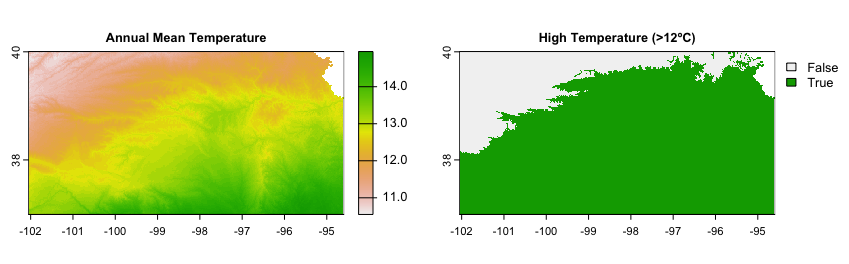
\includegraphics[width=1\linewidth]{SoilFER-Training-Resources/01_outputs/high_temp} \caption{Reclassification of raster values with map algebra}\label{fig:unnamed-chunk-10}
\end{figure}

\subparagraph*{Combining environmental (Raster) and soil (Vector) information}\label{combining-environmental-raster-and-soil-vector-information}
\addcontentsline{toc}{subparagraph}{Combining environmental (Raster) and soil (Vector) information}

In Digital Soil Mapping, the calibration of statistical models need to link the analytical properties of soils with the environmental covariates. This is done by their overlapping position. To link soil observations (points) with environmental covariates (rasters), extract raster values at sample locations using \texttt{extract()}.

\begin{Shaded}
\begin{Highlighting}[]
\CommentTok{\# Extract covariate values at point locations (soils\_sf)}
\NormalTok{cov\_values }\OtherTok{\textless{}{-}} \FunctionTok{extract}\NormalTok{(covs, soil\_sf)}
\end{Highlighting}
\end{Shaded}

The new object \texttt{cov\_values} is a data frame which does not have the original data of the sf object \texttt{soil\_sf}. A simple column bind command (\texttt{cbind}) can be used bind covariates to \texttt{soil\_sf}, which remains an sf object keeping geometry (coordinates) and all original columns, plus the covariate columns.

\begin{Shaded}
\begin{Highlighting}[]
\CommentTok{\# cov\_values includes an ID column in the first column}
\NormalTok{soil\_sf }\OtherTok{\textless{}{-}} \FunctionTok{cbind}\NormalTok{(soil\_sf, cov\_values[ , }\SpecialCharTok{{-}}\DecValTok{1}\NormalTok{, }\AttributeTok{drop =} \ConstantTok{FALSE}\NormalTok{])}
\end{Highlighting}
\end{Shaded}

This dataset contains all the information to be used in further analyses of Sampling Design and calibration of Digital Soil Mapping models.

\subsubsection{Calculation of Soil--Climate Rasters (Newhall Simulation Model)}\label{calculation-of-soilclimate-rasters-newhall-simulation-model}

The Newhall Simulation Model (NSM) is a water-balance--based model originally developed to estimate soil moisture and soil temperature regimes from climate and site characteristics (\citeproc{ref-NewhallBerdanier1996}{Newhall and Berdanier, 1996}). It simulates the seasonal dynamics of soil water storage and temperature using monthly climate inputs and simple soil physical assumptions. The resulting regime classes (e.g., ustic, udic, xeric; and temperature regimes such as mesic or thermic) are widely used in soil survey and soil classification contexts, and they are also useful as environmental descriptors in DSM workflows.

In this tutorial, we use the R implementation of the NSM available in the \texttt{\{jNSMR\}} package.

The model requires several raster layers as inputs:

\begin{itemize}
\item
  Monthly precipitation (pJan \ldots{} pDec): drives water inputs into the soil water balance.
\item
  Monthly temperature (tJan \ldots{} tDec): controls evapotranspiration demand and soil temperature dynamics.
\end{itemize}

In addition to monthly precipitation and temperature, the Newhall Simulation Model also requires site descriptors that influence soil water balance and seasonality:

\begin{itemize}
\item
  Elevation (DEM): to account for altitude-related effects on temperature (and therefore evapotranspiration and soil temperature patterns).
\item
  Available Water Capacity (AWC): to represent, in mm, how much water the soil can store (typically for a reference depth, e.g., 0--200 cm), which controls how quickly soils dry after rainfall.
\item
  Longitude and latitude: to provide each grid cell's geographic position, supporting calculations that depend on seasonal timing and solar geometry (e.g., daylength patterns and the timing of solstices used in some Newhall metrics such as `days after summer solstice' or `after winter solstice').
\end{itemize}

This workflow processes monthly temperature and precipitation data from large time series (1981--2023), computes long-term monthly averages, and prepares all the above described rasters in a stack to run the Newhall soil--climate model (via \texttt{\{jNSMR\}}). The output includes soil-climate diagnostics and regime classifications (e.g., temperature and moisture regimes), which can be used as covariates in Sampling Design and Digital Soil Mapping.

\paragraph*{Environment setup}\label{environment-setup}
\addcontentsline{toc}{paragraph}{Environment setup}

The first step is to prepare the Environment setup (loading packages, define path to data files, and set the CRS).

\begin{Shaded}
\begin{Highlighting}[]
\CommentTok{\# Packages}
\FunctionTok{library}\NormalTok{(terra)}
\FunctionTok{library}\NormalTok{(sf)}
\FunctionTok{library}\NormalTok{(dplyr)}
\FunctionTok{library}\NormalTok{(jNSMR)}

\CommentTok{\# Target CRS for the workflow (use a projected CRS for analysis)}
\NormalTok{epsg }\OtherTok{\textless{}{-}} \StringTok{"EPSG:3857"}   \CommentTok{\# Web Mercator (meters). Replace if needed.}
\NormalTok{agg.factor }\OtherTok{\textless{}{-}} \DecValTok{1}       \CommentTok{\# Optional aggregation to speed up Newhall calculations (1 = no aggregation)}
\end{Highlighting}
\end{Shaded}

\paragraph*{Prepare monthly average rasters of climatic data}\label{prepare-monthly-average-rasters-of-climatic-data}
\addcontentsline{toc}{paragraph}{Prepare monthly average rasters of climatic data}

TerraClimate files contain large time series (1981-2020) of climatic records. Monthly temperature and precipitation averages from these series must be calculated as independent raster files. Temperature in this dataset if scaled (e.g., ×10) to avoid decimal point data and save storage space this it has to be adjusted to real values. The following chunk computes the averages for every month across all years, producing a 12-layer raster stack of monthly averages.

\begin{Shaded}
\begin{Highlighting}[]
\CommentTok{\# Monthly temperature time series (multi{-}year, monthly layers)}
\NormalTok{tmp }\OtherTok{\textless{}{-}} \FunctionTok{rast}\NormalTok{(}\FunctionTok{paste0}\NormalTok{(training\_dir,}\StringTok{"TerraClimate\_AvgTemp\_1981\_2023\_KANSAS.tif"}\NormalTok{))}

\CommentTok{\# Number of years in the stack (assuming complete years)}
\NormalTok{nyears }\OtherTok{\textless{}{-}} \FunctionTok{nlyr}\NormalTok{(tmp) }\SpecialCharTok{/} \DecValTok{12}

\CommentTok{\# Monthly means across all years}
\NormalTok{temp\_list }\OtherTok{\textless{}{-}} \FunctionTok{vector}\NormalTok{(}\StringTok{"list"}\NormalTok{, }\DecValTok{12}\NormalTok{)}
\NormalTok{tmp\_ref }\OtherTok{\textless{}{-}}\NormalTok{ tmp[[}\DecValTok{1}\NormalTok{]]  }\CommentTok{\# reference layer for initializing}
\ControlFlowTok{for}\NormalTok{(i }\ControlFlowTok{in} \DecValTok{1}\SpecialCharTok{:}\DecValTok{12}\NormalTok{)\{}
\NormalTok{  var\_sum }\OtherTok{\textless{}{-}}\NormalTok{ tmp\_ref }\SpecialCharTok{*} \DecValTok{0}
\NormalTok{  k }\OtherTok{\textless{}{-}}\NormalTok{ i}
  \ControlFlowTok{for}\NormalTok{(j }\ControlFlowTok{in} \DecValTok{1}\SpecialCharTok{:}\NormalTok{nyears)\{}
\NormalTok{    var\_sum }\OtherTok{\textless{}{-}}\NormalTok{ var\_sum }\SpecialCharTok{+}\NormalTok{ tmp[[k]]}
\NormalTok{    k }\OtherTok{\textless{}{-}}\NormalTok{ k }\SpecialCharTok{+} \DecValTok{12}
\NormalTok{  \}}
\NormalTok{  temp\_list[[i]] }\OtherTok{\textless{}{-}}\NormalTok{ var\_sum }\SpecialCharTok{/}\NormalTok{ nyears}
\NormalTok{\}}
\CommentTok{\# Convert to stack}
\NormalTok{Temp\_Stack }\OtherTok{\textless{}{-}} \FunctionTok{rast}\NormalTok{(temp\_list) }\SpecialCharTok{*} \FloatTok{0.1}  \CommentTok{\# convert scaled values to °C (×0.1)}
\CommentTok{\# Write to disk}
\FunctionTok{writeRaster}\NormalTok{(Temp\_Stack, }\StringTok{"03\_outputs/module1/Temp\_Stack\_monthlyMean.tif"}\NormalTok{, }\AttributeTok{overwrite =} \ConstantTok{TRUE}\NormalTok{)}


\CommentTok{\# Monthly precipitation time series (multi{-}year, monthly layers)}
\NormalTok{prec\_mm }\OtherTok{\textless{}{-}} \FunctionTok{rast}\NormalTok{(}\FunctionTok{paste0}\NormalTok{(training\_dir,}\StringTok{"TerraClimate\_Precip\_1981\_2023\_KANSAS.tif"}\NormalTok{))}
\CommentTok{\# Number of years in the stack (assuming complete years}
\NormalTok{nyears }\OtherTok{\textless{}{-}} \FunctionTok{nlyr}\NormalTok{(prec\_mm) }\SpecialCharTok{/} \DecValTok{12}
\CommentTok{\# Monthly means across all years}
\NormalTok{prec\_list }\OtherTok{\textless{}{-}} \FunctionTok{vector}\NormalTok{(}\StringTok{"list"}\NormalTok{, }\DecValTok{12}\NormalTok{)}
\NormalTok{pre\_ref }\OtherTok{\textless{}{-}}\NormalTok{ prec\_mm[[}\DecValTok{1}\NormalTok{]] }\CommentTok{\# reference layer for initializing}
\ControlFlowTok{for}\NormalTok{(i }\ControlFlowTok{in} \DecValTok{1}\SpecialCharTok{:}\DecValTok{12}\NormalTok{)\{}
\NormalTok{  var\_sum }\OtherTok{\textless{}{-}}\NormalTok{ pre\_ref }\SpecialCharTok{*} \DecValTok{0}
\NormalTok{  k }\OtherTok{\textless{}{-}}\NormalTok{ i}
  \ControlFlowTok{for}\NormalTok{(j }\ControlFlowTok{in} \DecValTok{1}\SpecialCharTok{:}\NormalTok{nyears)\{}
\NormalTok{    var\_sum }\OtherTok{\textless{}{-}}\NormalTok{ var\_sum }\SpecialCharTok{+}\NormalTok{ prec\_mm[[k]]}
\NormalTok{    k }\OtherTok{\textless{}{-}}\NormalTok{ k }\SpecialCharTok{+} \DecValTok{12}
\NormalTok{  \}}
\NormalTok{  prec\_list[[i]] }\OtherTok{\textless{}{-}}\NormalTok{ var\_sum }\SpecialCharTok{/}\NormalTok{ nyears}
\NormalTok{\}}
\CommentTok{\# Convert to stack}
\NormalTok{Prec\_Stack }\OtherTok{\textless{}{-}} \FunctionTok{rast}\NormalTok{(prec\_list)}
\CommentTok{\# Write to disk}
\FunctionTok{writeRaster}\NormalTok{(Prec\_Stack, }\StringTok{"03\_outputs/module1/Prec\_Stack\_monthlyMean.tif"}\NormalTok{, }\AttributeTok{overwrite =} \ConstantTok{TRUE}\NormalTok{)}
\end{Highlighting}
\end{Shaded}

\paragraph*{Prepare monthly average stack of climatic data}\label{prepare-monthly-average-stack-of-climatic-data}
\addcontentsline{toc}{paragraph}{Prepare monthly average stack of climatic data}

NSM expects monthly precipitation and temperature layers with specific, predefined layer names.

\begin{Shaded}
\begin{Highlighting}[]
\CommentTok{\# Load outputs (reuse objects from above)}
\NormalTok{Prec\_Stack }\OtherTok{\textless{}{-}} \FunctionTok{rast}\NormalTok{(}\StringTok{"03\_outputs/module1/Prec\_Stack\_monthlyMean.tif"}\NormalTok{)}
\NormalTok{Temp\_Stack }\OtherTok{\textless{}{-}} \FunctionTok{rast}\NormalTok{(}\StringTok{"03\_outputs/module1/Temp\_Stack\_monthlyMean.tif"}\NormalTok{)}


\FunctionTok{names}\NormalTok{(Prec\_Stack) }\OtherTok{\textless{}{-}} \FunctionTok{c}\NormalTok{(}\StringTok{"pJan"}\NormalTok{,}\StringTok{"pFeb"}\NormalTok{,}\StringTok{"pMar"}\NormalTok{,}\StringTok{"pApr"}\NormalTok{,}\StringTok{"pMay"}\NormalTok{,}\StringTok{"pJun"}\NormalTok{,}\StringTok{"pJul"}\NormalTok{,}\StringTok{"pAug"}\NormalTok{,}\StringTok{"pSep"}\NormalTok{,}\StringTok{"pOct"}\NormalTok{,}\StringTok{"pNov"}\NormalTok{,}\StringTok{"pDec"}\NormalTok{)}
\FunctionTok{names}\NormalTok{(Temp\_Stack) }\OtherTok{\textless{}{-}} \FunctionTok{c}\NormalTok{(}\StringTok{"tJan"}\NormalTok{,}\StringTok{"tFeb"}\NormalTok{,}\StringTok{"tMar"}\NormalTok{,}\StringTok{"tApr"}\NormalTok{,}\StringTok{"tMay"}\NormalTok{,}\StringTok{"tJun"}\NormalTok{,}\StringTok{"tJul"}\NormalTok{,}\StringTok{"tAug"}\NormalTok{,}\StringTok{"tSep"}\NormalTok{,}\StringTok{"tOct"}\NormalTok{,}\StringTok{"tNov"}\NormalTok{,}\StringTok{"tDec"}\NormalTok{)}

\NormalTok{combined\_stack }\OtherTok{\textless{}{-}} \FunctionTok{c}\NormalTok{(Prec\_Stack, Temp\_Stack)}
\FunctionTok{writeRaster}\NormalTok{(combined\_stack, }\StringTok{"03\_outputs/module1/climate\_vars.tif"}\NormalTok{, }\AttributeTok{overwrite =} \ConstantTok{TRUE}\NormalTok{)}
\end{Highlighting}
\end{Shaded}

\paragraph*{Prepare site descriptors that influence soil water balance and seasonality}\label{prepare-site-descriptors-that-influence-soil-water-balance-and-seasonality}
\addcontentsline{toc}{paragraph}{Prepare site descriptors that influence soil water balance and seasonality}

In addition to monthly precipitation and temperature, NSM uses a number of site descriptors influencing soil climate:

\begin{itemize}
\item
  Elevation (DEM).
\item
  Available Water Capacity (AWC).
\item
  Longitude and latitude.
\end{itemize}

These raster layers are obtained from different sources thus, their geometry has to be harmonized to create a unique raster stack for the calculations.

\begin{Shaded}
\begin{Highlighting}[]
\CommentTok{\# DEM}
\CommentTok{\# Read raster}
\NormalTok{elev }\OtherTok{\textless{}{-}} \FunctionTok{rast}\NormalTok{(}\FunctionTok{paste0}\NormalTok{(training\_dir,}\StringTok{"DEM\_KANSAS.tif"}\NormalTok{))}
\CommentTok{\# Align CRS to the common EPSG}
\ControlFlowTok{if}\NormalTok{(}\FunctionTok{crs}\NormalTok{(elev) }\SpecialCharTok{!=}\NormalTok{ epsg) elev }\OtherTok{\textless{}{-}} \FunctionTok{project}\NormalTok{(elev, epsg, }\AttributeTok{method =} \StringTok{"near"}\NormalTok{)}

\CommentTok{\# AWC (0–200 cm, in mm)}
\CommentTok{\# Read raster}
\NormalTok{awc }\OtherTok{\textless{}{-}} \FunctionTok{rast}\NormalTok{(}\FunctionTok{paste0}\NormalTok{(training\_dir,}\StringTok{"awc\_KANSAS.tif"}\NormalTok{))}
\CommentTok{\# Align CRS to the common EPSG}
\ControlFlowTok{if}\NormalTok{(}\FunctionTok{crs}\NormalTok{(awc) }\SpecialCharTok{!=}\NormalTok{ epsg) awc }\OtherTok{\textless{}{-}} \FunctionTok{project}\NormalTok{(awc, epsg, }\AttributeTok{method =} \StringTok{"near"}\NormalTok{)}
\CommentTok{\# Align geometries with the DEM raster}
\NormalTok{awc }\OtherTok{\textless{}{-}} \FunctionTok{resample}\NormalTok{(awc, elev)}
\CommentTok{\# Define name}
\FunctionTok{names}\NormalTok{(awc) }\OtherTok{\textless{}{-}} \StringTok{"awc"}

\CommentTok{\# Temperature and Precipitation}
\CommentTok{\# Read climate stack}
\NormalTok{newhall }\OtherTok{\textless{}{-}} \FunctionTok{rast}\NormalTok{(}\StringTok{"03\_outputs/module1/climate\_vars.tif"}\NormalTok{)}
\CommentTok{\# Align CRS to the common EPSG}
\ControlFlowTok{if}\NormalTok{(}\FunctionTok{crs}\NormalTok{(newhall) }\SpecialCharTok{!=}\NormalTok{ epsg) newhall }\OtherTok{\textless{}{-}} \FunctionTok{project}\NormalTok{(newhall, epsg, }\AttributeTok{method =} \StringTok{"near"}\NormalTok{)}
\CommentTok{\# Align geometries with the DEM raster}
\NormalTok{newhall }\OtherTok{\textless{}{-}} \FunctionTok{resample}\NormalTok{(newhall, elev)}

\CommentTok{\# Longitude and Latitude }
\CommentTok{\# calculate lon/lat from the climate stack}
\NormalTok{newhall}\SpecialCharTok{$}\NormalTok{lonDD }\OtherTok{\textless{}{-}} \FunctionTok{init}\NormalTok{(newhall[[}\DecValTok{1}\NormalTok{]], }\StringTok{"x"}\NormalTok{)}
\NormalTok{newhall}\SpecialCharTok{$}\NormalTok{latDD }\OtherTok{\textless{}{-}} \FunctionTok{init}\NormalTok{(newhall[[}\DecValTok{1}\NormalTok{]], }\StringTok{"y"}\NormalTok{)}

\CommentTok{\# Mask climate stack to DEM valid area and add DEM/AWC to the stack}
\NormalTok{newhall }\OtherTok{\textless{}{-}} \FunctionTok{mask}\NormalTok{(newhall, elev)}
\NormalTok{newhall}\SpecialCharTok{$}\NormalTok{awc  }\OtherTok{\textless{}{-}}\NormalTok{ awc}
\NormalTok{newhall}\SpecialCharTok{$}\NormalTok{elev }\OtherTok{\textless{}{-}}\NormalTok{ elev}

\CommentTok{\# Save full NSM input stack}
\FunctionTok{writeRaster}\NormalTok{(newhall, }\StringTok{"03\_outputs/module1/climate\_newhall\_vars.tif"}\NormalTok{, }\AttributeTok{overwrite =} \ConstantTok{TRUE}\NormalTok{)}
\end{Highlighting}
\end{Shaded}

\paragraph*{Calculate NSM outputs}\label{calculate-nsm-outputs}
\addcontentsline{toc}{paragraph}{Calculate NSM outputs}

Depending on resolution and extent, the calculation of the NSM can take hours. To reduce runtime you may aggregate the input stack (optional), then run \texttt{newhall\_batch()} with multiple cores.

\begin{Shaded}
\begin{Highlighting}[]
\CommentTok{\# Read the full Newhall input stack}
\NormalTok{newhall }\OtherTok{\textless{}{-}} \FunctionTok{rast}\NormalTok{(}\StringTok{"03\_outputs/module1/cclimate\_newhall\_vars.tif"}\NormalTok{)}

\CommentTok{\# Optional: aggregate to speed up (e.g., fact = 2, 3, ...)}
\CommentTok{\# newhall \textless{}{-} aggregate(newhall, fact = agg.factor)}

\FunctionTok{system.time}\NormalTok{(\{}
\NormalTok{  newhall\_results }\OtherTok{\textless{}{-}}\NormalTok{ jNSMR}\SpecialCharTok{::}\FunctionTok{newhall\_batch}\NormalTok{(newhall, }\AttributeTok{cores =} \DecValTok{4}\NormalTok{)}
\NormalTok{\})}
\end{Highlighting}
\end{Shaded}

\paragraph*{Inspect and export results (compact outputs)}\label{inspect-and-export-results-compact-outputs}
\addcontentsline{toc}{paragraph}{Inspect and export results (compact outputs)}

The NSM output includes the following layers:

\begin{tabular}{l|l|l}
\hline
Layer & Units & Description\\
\hline
annualRainfall & mm/yr & Total precipitation accumulated over the year.\\
\hline
waterHoldingCapacity & mm & Soil water-holding capacity used by the model (plant-available storage over the modeled profile/control section).\\
\hline
annualWaterBalance & mm/yr & Net annual water balance (precipitation − potential evapotranspiration) summed over the year; positive = surplus, negative = deficit.\\
\hline
annualPotentialEvapotranspiration & mm/yr & Total annual potential evapotranspiration (atmospheric evaporative demand) summed over the year.\\
\hline
summerWaterBalance & mm (summer period) & Net water balance during the model’s summer period (precipitation − potential evapotranspiration) for that season.\\
\hline
dryDaysAfterSummerSolstice & days & Number of days classified as dry after the summer solstice (indicator of summer dryness duration).\\
\hline
moistDaysAfterWinterSolstice & days & Number of days classified as moist after the winter solstice (indicator of post-winter moisture duration).\\
\hline
numCumulativeDaysDry & days & Cumulative number of dry days across the year (sum of days meeting the model’s dry condition).\\
\hline
numCumulativeDaysMoistDry & days & Cumulative number of moist-dry (intermediate) days across the year.\\
\hline
numCumulativeDaysMoist & days & Cumulative number of moist days across the year.\\
\hline
numCumulativeDaysDryOver5C & days & Cumulative number of dry days when temperature is > 5 °C.\\
\hline
numCumulativeDaysMoistDryOver5C & days & Cumulative number of moist-dry days when temperature is > 5 °C.\\
\hline
numCumulativeDaysMoistOver5C & days & Cumulative number of moist days when temperature is > 5 °C.\\
\hline
numConsecutiveDaysMoistInSomeParts & days & Consecutive days when the soil is moist in some part of the control section (persistence of partial-profile moisture).\\
\hline
numConsecutiveDaysMoistInSomePartsOver8C & days & Consecutive days when the soil is moist in some part of the control section and temperature is > 8 °C.\\
\hline
temperatureRegime & class & Categorical soil temperature regime output (e.g., mesic, thermic), derived from the model’s temperature criteria.\\
\hline
moistureRegime & class & Categorical soil moisture regime output (e.g., udic, ustic, xeric), derived from the model’s moisture criteria.\\
\hline
regimeSubdivision1 & class & Van Wambeke modifier (Part 1): a simple qualifier such as Wet/Dry/Typic/Weak/Extreme that refines the moisture regime.\\
\hline
regimeSubdivision2 & class & Van Wambeke base term (Part 2): the main regime term (often Temp* or Trop* forms like Tempustic/Tropustic or Tempudic/Tropudic). Combine with Part 1 to get the full label (e.g., 'Wet Tempustic').\\
\hline
\end{tabular}

The final step is to inspect, mask, and export NSM outputs for use in subsequent analyses.\\
We mask the model outputs using the annual rainfall layer as a validity template, which helps remove spurious values in areas where the climate inputs are undefined (e.g., open water or NoData zones in the precipitation surface).

\begin{Shaded}
\begin{Highlighting}[]
\CommentTok{\# Build a validity mask from the precipitation layer}
\NormalTok{mask\_valid }\OtherTok{\textless{}{-}} \SpecialCharTok{!}\FunctionTok{is.na}\NormalTok{(newhall\_results}\SpecialCharTok{$}\NormalTok{annualRainfall)}
\CommentTok{\# Apply the mask to all NSM layers}
\NormalTok{results }\OtherTok{\textless{}{-}} \FunctionTok{mask}\NormalTok{(newhall\_results, mask\_valid)}
\CommentTok{\# Quick inspection}
\CommentTok{\# {-}{-}{-}{-}{-}{-}{-}{-}{-}{-}{-}{-}{-}{-}{-}{-}{-}{-}{-}{-}{-}{-}{-}{-}{-}{-}{-}{-}{-}{-}{-}{-}{-}{-}{-}{-}{-}{-}{-}{-}{-}{-}{-}{-}{-}{-}{-}{-}{-}{-}{-}{-}{-}{-}{-}{-}{-}{-}{-}{-}{-}{-}{-}{-}{-}{-}{-}}
\FunctionTok{names}\NormalTok{(results)}
\FunctionTok{plot}\NormalTok{(results[}\DecValTok{1}\SpecialCharTok{:}\DecValTok{6}\NormalTok{])}

\CommentTok{\# Export to GeoTIFF}
\FunctionTok{writeRaster}\NormalTok{(results, }\StringTok{"03\_outputs/module1/newhall.tif"}\NormalTok{, }\AttributeTok{overwrite =} \ConstantTok{TRUE}\NormalTok{)}

\CommentTok{\# Optional: compact integer exports}
\CommentTok{\#    Multiply by 10 to preserve 1 decimal place, then store as integer.}
\CommentTok{\#    (Useful to reduce file size when decimals are not critical.)}

\NormalTok{results\_intx10 }\OtherTok{\textless{}{-}} \FunctionTok{app}\NormalTok{(results, }\ControlFlowTok{function}\NormalTok{(x) }\FunctionTok{as.integer}\NormalTok{(}\FunctionTok{round}\NormalTok{(x }\SpecialCharTok{*} \DecValTok{10}\NormalTok{)))}
\FunctionTok{writeRaster}\NormalTok{(results\_intx10, }\StringTok{"03\_outputs/module1/newhall\_intx10.tif"}\NormalTok{, }\AttributeTok{overwrite =} \ConstantTok{TRUE}\NormalTok{)}
\end{Highlighting}
\end{Shaded}

The raster stack \texttt{newhall\_results} contains the NSM outputs, which can be used as covariates in both the Sampling Design and Digital Soil Mapping workflows.

\chapter{Sampling design for soil surveys}\label{sampling-design-for-soil-surveys}

Placeholder

\section{Introduction}\label{introduction-ssd}

\section{Sampling methodologies for soil spatial survey}\label{sampling-theory}

\subsection{Selection of the sampling methodology}\label{selection-methods}

\subsection{Inference Methods}\label{inference-methods}

\subsection{Purpose of Sampling}\label{sampling-purpose}

\subsection{Sampling Design Types}\label{design-types}

\subsection{Example: Soils4Africa Sampling Design}\label{soils4africa-example}

\section{SoilFER Sampling Design}\label{soilfer-design}

\subsection{Soil Properties}\label{soil-properties}

\subsection{Environmental Covariates}\label{env-covariates}

\subsection{Understanding the Methodology}\label{methodology}

\subsubsection{PSU Selection Process}\label{psu-selection-process}

\subsubsection{SSU and TSU Selection Process}\label{ssu-tsu-selection}

\subsubsection{Site Identification System}\label{site-id}

\section{Tutorial using R}\label{tutorial}

\subsection{Setting up the environment}\label{setup}

\subsection{Install required libraries}\label{install-libraries}

\subsection{Define variables and parameters}\label{define-parameters}

\subsubsection{Country ISO code}\label{country-iso-code}

\subsubsection{Land-use type}\label{land-use-type}

\subsubsection{File paths}\label{file-paths}

\subsubsection{Coordinate reference system}\label{coordinate-reference-system}

\subsubsection{Sample size calculation}\label{sample-size-calculation}

\subsubsection{Sampling unit definitions}\label{sampling-unit-definitions}

\subsubsection{Algorithm parameters}\label{algorithm-parameters}

\subsection{Custom functions}\label{custom-functions}

\subsubsection{Covariate Space Coverage (CSIS)}\label{covariate-space-coverage-csis}

\subsubsection{K-means with progress reporting}\label{k-means-with-progress-reporting}

\subsubsection{TSU generation}\label{tsu-generation}

\subsection{Load country boundaries and legacy data}\label{load-boundaries}

\subsubsection{Visualize boundaries and legacy data}\label{visualize-boundaries-and-legacy-data}

\subsection{Load environmental covariates for PSUs}\label{load-covariates-psu}

\subsubsection{Protected areas mask (exclude from sampling)}\label{protected-areas-mask-exclude-from-sampling}

\subsubsection{Slope mask (exclude steep terrain)}\label{slope-mask-exclude-steep-terrain}

\subsubsection{Ecoregions / Geology data (for stratification)}\label{ecoregions-geology-data-for-stratification}

\subsubsection{Geomorphology data (for stratification)}\label{geomorphology-data-for-stratification}

\subsubsection{Environmental covariates created/retrieved from previous Chapter}\label{environmental-covariates-createdretrieved-from-previous-chapter}

\subsubsection{Load and process soil-climate data (Newhall)}\label{load-and-process-soil-climate-data-newhall}

\subsubsection{Convert soil-climate regimes to dummy variables}\label{convert-soil-climate-regimes-to-dummy-variables}

\subsubsection{Integrating all layers and finalising the Covariate Stack}\label{integrating-all-layers-and-finalising-the-covariate-stack}

\subsection{Principal Component Analysis (PCA)}\label{pca}

\subsection{Load and prepare land-use data}\label{sec-landuse}

\subsection{Create Primary Sampling Units (PSU Grid)}\label{create-psu-grid}

\subsection{Select PSUs with sufficient land-use coverage}\label{select-psus}

\subsection{Calculate optimal sample size}\label{sec-optimal-sample-size}

\subsection{Select PSUs using Covariate Space Coverage (CSC)}\label{sec-select-psus-csc}

\subsection{Compute SSUs and TSUs}\label{compute-ssu-tsu}

\subsection{Compute Alternative PSUs}\label{alternative-psus}

\subsection{Assign Country-Wide Unique IDs}\label{assign-unique-ids}

\subsection{Field sampling protocol}\label{field-protocol}

\subsection*{Appendices}\label{appendices}
\addcontentsline{toc}{subsection}{Appendices}

\subsubsection*{Appendix A: Software and Data Sources}\label{appendix-a-software-and-data-sources}
\addcontentsline{toc}{subsubsection}{Appendix A: Software and Data Sources}

\subsubsection*{Appendix B: Troubleshooting Common Issues}\label{appendix-b-troubleshooting-common-issues}
\addcontentsline{toc}{subsubsection}{Appendix B: Troubleshooting Common Issues}

\subsubsection*{Appendix C: Acronyms and Abbreviations}\label{appendix-c-acronyms-and-abbreviations}
\addcontentsline{toc}{subsubsection}{Appendix C: Acronyms and Abbreviations}

\chapter{Digital Soil Mapping}\label{digital-soil-mapping}

Placeholder

\section{Fundamentals of Digital Soil Mapping}\label{fundamentals-of-digital-soil-mapping}

\subsection{Introduction to Digital Soil Mapping}\label{introduction-to-digital-soil-mapping}

\subsection*{The SCORPAN Framework}\label{SCORPAN-Framework}
\addcontentsline{toc}{subsection}{The SCORPAN Framework}

\subsection{Statistical Theory for Predictive Soil Mapping}\label{statistical-theory-for-predictive-soil-mapping}

\subsubsection{Mechanistic versus Empirical Approaches}\label{mechanistic-versus-empirical-approaches}

\subsubsection{Sources of Residual Variance}\label{sources-of-residual-variance}

\subsubsection{Covariates as Proxies of Soil-Forming Factors}\label{covariates-as-proxies-of-soil-forming-factors}

\subsubsection{The Universal Model of Soil Variation}\label{the-universal-model-of-soil-variation}

\subsubsection{Extending the Model: Space, Depth, and Time (3D+T)}\label{extending-the-model-space-depth-and-time-3dt}

\subsection{Types of Soil Variables}\label{types-of-soil-variables}

\subsection{Prediction Methods}\label{prediction-methods}

\subsection{Nonlinearity and Uncertainty}\label{nonlinearity-and-uncertainty}

\section{Practical Implementation Example}\label{practical-implementation-example}

\subsection{Overview}\label{overview}

\subsection{Setup and Packages}\label{setup-and-packages}

\subsection{Load covariates}\label{load-covariates}

\subsection{Load and transform soil data}\label{load-and-transform-soil-data}

\subsubsection{Estimate bulk density with a pedotransfer function}\label{estimate-bulk-density-with-a-pedotransfer-function}

\subsection{Merge soil data and covariate values}\label{merge-soil-data-and-covariate-values}

\subsection{Feature selection with Boruta}\label{feature-selection-with-boruta}

\subsection{Train the Quantile Regression Forest model}\label{train-the-quantile-regression-forest-model}

\subsubsection{From Random Forest to Quantile Regression Forest}\label{from-random-forest-to-quantile-regression-forest}

\subsubsection{Cross-validation setup}\label{cross-validation-setup}

\subsubsection{Hyperparameter grid}\label{hyperparameter-grid}

\subsubsection{Train the model}\label{train-the-model}

\subsection{Accuracy assessment}\label{accuracy-assessment}

\subsubsection{Observed vs predicted plot}\label{observed-vs-predicted-plot}

\subsubsection{Save outputs}\label{save-outputs}

\subsection{Reload the workspace}\label{reload-the-workspace}

\subsection{Spatial prediction (tiled)}\label{spatial-prediction-tiled}

\subsubsection{Create tile grid}\label{create-tile-grid}

\subsubsection{Prepare model for prediction}\label{prepare-model-for-prediction}

\subsubsection{Prediction for one tile}\label{prediction-for-one-tile}

\subsubsection{Prediction at all tiles}\label{prediction-at-all-tiles}

\subsection{Mosaic tiles into final maps}\label{mosaic-tiles-into-final-maps}

\chapter{Soil Spectroscopy for Digital Soil Mapping}\label{soil-spectroscopy-for-digital-soil-mapping}

Placeholder

\section{Introduction}\label{introduction-1}

\subsection{Rationale}\label{rationale}

\subsection{Including Spectroscopic Predictions in Digital Soil Mapping}\label{including-spectroscopic-predictions-in-digital-soil-mapping}

\section{Workflow overview}\label{workflow-overview}

\section{Generating DRS-derived soil property observations for DSM}\label{generating-drs-derived-soil-property-observations-for-dsm}

\subsection{How to get the data}\label{how-to-get-the-data}

\subsection{Main R packages used here}\label{main-r-packages-used-here}

\subsection{Load and plot the DRS data}\label{load-and-plot-the-drs-data}

\subsection{Preprocessing of the soil spectra}\label{preprocessing-of-the-soil-spectra}

\subsection{SOC prediction from DRS spectra with uncertainty estimation}\label{soc-prediction-from-drs-spectra-with-uncertainty-estimation}

\subsubsection{A quick note on calibration sampling}\label{a-quick-note-on-calibration-sampling}

\subsubsection{Select a representative subset of calibration samples for model fitting}\label{select-a-representative-subset-of-calibration-samples-for-model-fitting}

\subsubsection{Model calibration}\label{model-calibration}

\subsubsection{DRS-based prediction and uncertainty estimation for non-calibration samples}\label{drs-based-prediction-and-uncertainty-estimation-for-non-calibration-samples}

\section{Assembling the augmented dataset of laboratory measurements and DRS-based predictions}\label{assembling-the-augmented-dataset-of-laboratory-measurements-and-drs-based-predictions}

\section{Uncertainty of the conventional laboratory measurement}\label{uncertainty-of-the-conventional-laboratory-measurement}

\section{Depth harmonization of predictions and uncertainties}\label{depth-harmonization-of-predictions-and-uncertainties}

\subsection{Reference dataset}\label{reference-dataset}

\subsection{Augmented dataset}\label{augmented-dataset}

\section{Digital soil mapping}\label{digital-soil-mapping-1}

\subsection{Preparation of the covariates}\label{preparation-of-the-covariates}

\subsection{DSM model training of SOC with DRS-augmented data}\label{dsm-model-training-of-soc-with-drs-augmented-data}

\subsubsection{Deriving observation weights}\label{deriving-observation-weights}

\subsubsection{Baseline DSM model using laboratory data}\label{baseline-dsm-model-using-laboratory-data}

\subsubsection{DSM model using DRS-augmented data}\label{dsm-model-using-drs-augmented-data}

\subsection{Model validation}\label{model-validation}

\subsubsection{Weighted performance metrics}\label{weighted-performance-metrics}

\subsubsection{Cross-validating the models}\label{cross-validating-the-models}

\section{Additional activities for further exploration}\label{additional-activities-for-further-exploration}

\subsection{What is the optimal number of samples for DRS model calibration?}\label{what-is-the-optimal-number-of-samples-for-drs-model-calibration}

\subsubsection{Step 1: Principal component analysis of the processed spectra}\label{step-1-principal-component-analysis-of-the-processed-spectra}

\subsubsection{Step 2: Kernel density estimates for the full population}\label{step-2-kernel-density-estimates-for-the-full-population}

\subsubsection{Step 3: MSD across calibration set sizes}\label{step-3-msd-across-calibration-set-sizes}

\subsubsection{Step 4: Visualising distributional convergence}\label{step-4-visualising-distributional-convergence}

\subsubsection{Step 5: Identifying the optimal calibration set size}\label{step-5-identifying-the-optimal-calibration-set-size}

\subsection{How does the number of DRS calibration samples affect DSM accuracy?}\label{how-does-the-number-of-drs-calibration-samples-affect-dsm-accuracy}

\subsubsection{Create the DRS calibration subsets}\label{create-the-drs-calibration-subsets}

\subsubsection{Calibrate DRS models and predict SOC for non-calibration samples}\label{calibrate-drs-models-and-predict-soc-for-non-calibration-samples}

\subsubsection{Assemble the augmented datasets}\label{assemble-the-augmented-datasets}

\subsubsection{Separate a fixed set of profiles for spatial validation}\label{separate-a-fixed-set-of-profiles-for-spatial-validation}

\subsubsection{Harmonise the DRS predictions to the 0--30 cm depth interval}\label{harmonise-the-drs-predictions-to-the-030-cm-depth-interval}

\subsubsection{Fit DSM models using the DRS-augmented datasets and compare the resulting SOC maps}\label{fit-dsm-models-using-the-drs-augmented-datasets-and-compare-the-resulting-soc-maps}

\subsubsection{Evaluate DSM accuracy on the held-out validation profiles}\label{evaluate-dsm-accuracy-on-the-held-out-validation-profiles}

\section{Additional exercises for independent exploration}\label{additional-exercises-for-independent-exploration}

\section{Summary}\label{summary}

\chapter{Soil Data Sharing and Dissemination}\label{soil-data-sharing-and-dissemination}

Placeholder

\section{Introduction}\label{introduction-2}

\section{The Soil Information System (SIS)}\label{the-soil-information-system-sis}

\subsection{What is a Spatial Data Infrastructure?}\label{what-is-a-spatial-data-infrastructure}

\subsection{What the SIS lets you do}\label{what-the-sis-lets-you-do}

\section{A node in the GloSIS federation}\label{glosis-node}

\section{Standardisation of soil point data: The GloSIS ISO 28258 database}\label{standardisation-of-soil-point-data-the-glosis-iso-28258-database}

\section{Standardisation of soil raster data}\label{standardisation-of-soil-raster-data}

\section{Getting started: accessing the SIS}\label{getting-started-accessing-the-sis}

\subsection{The map viewer}\label{the-map-viewer}

\subsection{The Admin Panel}\label{the-admin-panel}

\section{My account}\label{my-account}

\section{Administration}\label{administration}

\subsection{Settings}\label{settings}

\subsection{Users}\label{users}

\subsection{Software update}\label{software-update}

\subsection{GloSIS Federation}\label{glosis-federation}

\section{Publishing soil profile data from a CSV}\label{publishing-soil-profile-data-from-a-csv}

\subsection{Step 1 --- Upload the CSV file}\label{step-1-upload-the-csv-file}

\subsection{Step 2 --- Preview the data}\label{step-2-preview-the-data}

\subsection{Step 3 --- Describe the dataset (metadata)}\label{step-3-describe-the-dataset-metadata}

\subsection{Step 4 --- Standardise your columns}\label{step-4-standardise-your-columns}

\subsection{Step 5 --- Validate and ingest}\label{step-5-validate-and-ingest}

\section{Publishing raster maps}\label{publishing-raster-maps}

\subsection{Step 1 --- Select the GeoTIFF}\label{step-1-select-the-geotiff}

\subsection{Step 2 --- Location and project}\label{step-2-location-and-project}

\subsection{Step 3 --- Soil property and units}\label{step-3-soil-property-and-units}

\subsection{Step 4 --- Dates, depth and statistics}\label{step-4-dates-depth-and-statistics}

\subsection{Step 5 --- Licence, catalogue and authors}\label{step-5-licence-catalogue-and-authors}

\subsection{Step 6 --- Review and upload}\label{step-6-review-and-upload}

\section{The Raster Calculator}\label{the-raster-calculator}

\subsection{Creating a recipe}\label{creating-a-recipe}

\subsection{Adding input layers and thresholds}\label{adding-input-layers-and-thresholds}

\subsection{Running the recipe}\label{running-the-recipe}

\subsection{Inspecting the result}\label{inspecting-the-result}

\section{Exploring data in the map viewer}\label{explore-viewer}

\section{Dashboard}\label{dashboard}

\section{Summary}\label{summary-1}

\chapter*{References}\label{references}
\addcontentsline{toc}{chapter}{References}

\phantomsection\label{refs}
\begin{CSLReferences}{0}{0}
\bibitem[\citeproctext]{ref-amatulli2020_geomorpho90m}
\textbf{Amatulli, Gi., McInerney, D., Sethi, T., Strobl, P. \& Domisch, S.} 2020. Geomorpho90m - global high-resolution geomorphometry layers. OpenTopography. \url{https://doi.org/10.5069/G91R6NPX}

\bibitem[\citeproctext]{ref-brus2022b}
\textbf{Brus, D.J.} 2022. \emph{Spatial sampling with r}. Boca Raton, FL, Chapman \& Hall/CRC Press.

\bibitem[\citeproctext]{ref-gupta_zenodo_2019}
\textbf{Gupta, S. \& Hengl, T.} 2019. Soil available water capacity in mm derived for 5 standard layers (0-10, 10-30, 30-60, 60-100 and 100-200 cm) at 250 m resolution. Zenodo. \url{https://doi.org/10.5281/zenodo.2629148}

\bibitem[\citeproctext]{ref-hengl2019}
\textbf{Hengl, T. \& MacMillan, R.A.} 2019. \emph{Predictive soil mapping with r}. Wageningen, the Netherlands, OpenGeoHub foundation. (also available at \url{https://soilmapper.org/}).

\bibitem[\citeproctext]{ref-jenny1941}
\textbf{Jenny, H.} 1941. \emph{Factors of soil formation. A system of quantitative pedology}. New York, McGraw-Hill.

\bibitem[\citeproctext]{ref-NewhallBerdanier1996}
\textbf{Newhall, F. \& Berdanier, C.R.} 1996. Calculation of soil moisture regimes from the climatic record, p. 13. No. 46. Natural Resources Conservation Service.

\bibitem[\citeproctext]{ref-pebesma2023}
\textbf{Pebesma, E. \& Bivand, R.} 2021. Spatial data science with applications in r. \emph{Methods in Ecology and Evolution}, 12: 1620--1633. \url{https://doi.org/10.1111/2041-210X.13650}

\bibitem[\citeproctext]{ref-prieto2023}
\textbf{Prieto-Castrillo, F., Rodríguez-Rastrero, M., Yunta, F., Borondo, F. \& Borondo, J.} 2023. Disentangling jenny's equation by machine learning. \emph{Scientific Reports}, 13(1): 20916. \url{https://doi.org/10.1038/s41598-023-44171-x}

\bibitem[\citeproctext]{ref-zanaga2022_worldcover2021_v200}
\textbf{Zanaga, D., Van De Kerchove, R., Daems, D., De Keersmaecker, W., Brockmann, C., Kirches, G., Wevers, J., Cartus, O., Santoro, M., Fritz, S., Lesiv, M., Herold, M., Tsendbazar, N.-E., Xu, P., Ramoino, F. \& Arino, O.} 2022. ESA WorldCover 10 m 2021 v200. Zenodo. \url{https://doi.org/10.5281/zenodo.7254221}

\end{CSLReferences}

%\printindex

\includepdf{images/backcover.pdf}

\end{document}
